\documentclass[11pt]{My_preprint}


\title{Averaged equations for disperse multiphase flows}

\author[1,2]{Nicolas Fintzi}
\author[2]{Daniel Lhuillier}
\author[1]{Jean-Lou Pierson}
% \author[2]{Stephane Popinet}
\affil[1]{IFP Energies Nouvelles, Rond-point de l’changeur de Solaize, 69360 Solaize}
\affil[2]{Sorbonne Université, Institut Jean le Rond $\partial$’Alembert, 4 place Jussieu, 75252 PARIS CEDEX 05, France}

\begin{document}

\maketitle

\begin{abstract}
    This article presents a comprehensive study of the averaged equations for dispersed multiphase flows.
    We present a systematic derivation of a general averaged hybrid model that incorporates the influence of internal properties and surface properties of arbitrary particles dispersed in a continuous phase.
    The dispersed phase averaged equations are derived using two distinct formalism :
    the particle-average or Lagrangian formalism proposed by \citet{zhang1994ensemble,jackson1997locally};
    and the phase-average method, which is also employed for the continuous phase based on the approach of \citet{drew1983mathematical}. 
    The particle-phase averaged formalism yields the conventional linear conservation equations, as well as the less familiar moments' conservation equations.
    The primary contribution of this work is the demonstration of the equivalence between the particle-averaged and phase-averaged equations. 
    We show that the dispersed phase-averaged equation, is in fact a series expansion of the so-called particle-averaged moments equations. 
    The second contribution of this work is the derivation of the arbirary order moment equations of the particle phase in their most generalized form. 
    The ambition of the manuscript is to provide a set of equation adaptable to any kind of dispersed two phase flow and discuss the various form it can take depending on the particle nature. 
\end{abstract}




\section{Introduction}

%Dispersed multiphase flows are ubiquitous in chemical engineering processes. 
%Examples include gas-solid flows in fluidized bed reactors, liquid-liquid flows in liquid-liquid extractors, and bubbly flows in flotation processes. 
%Developing a versatile model capable of capturing the various nature of the dispersed multiphase flow is therefore essential.
%In this work we aim to bridge the existing gaps in current models by providing a unified and adaptable framework for any kind of dispersed multiphase flow problems including interfaccial transport equation.

Dispersed multiphase flows are encountered across a wide range of chemical engineering applications. 
These include gas-solid interactions in fluidized bed reactors , liquid-liquid flows in extractors, and gas-liquid bubbly flows in flotation processes. 
These systems exhibit a wide range of scales, from the size of individual inclusions (as small as a few micrometers) to the size of the reactor (often exceeding one meter), making fully resolved simulations computationally impractical. 
As a result, the current engineering practice relies on averaged equations of motion for both the dispersed and continuous phases. 
Therefore, developing a robust set of averaged equations that accurately captures the complexities of dispersed multiphase flows is essential. 
In this study, we aim to overcome the limitations of existing models by proposing a comprehensive set of averaged equations that can be applied to various types of dispersed multiphase flows, including interfacial transport processes.

%Due to the two many scales encountered in this process ranging from the particle size (from let'say 10 micrometer) to the reactor size (larger thant one meter) it appears to be unfeasible to model the process into play using fully resolved simulations.
%The current engineering practice is to relay on averaged set of equation of motion for both the dipsersed and continuous phase equation.
%Therefore, it is essential to develop a rigorous set of averaged equations that can accurately represent the diverse behaviors of dispersed multiphase flows. 
%In this study, our goal is to address the limitations of existing models by proposing a comprehensive averaged set of equations that can be applied to various kind of dispersed multiphase flow, including interfacial transport equations. %framework 

%Most of the averaged two-fluid models relies on the framework proposed by \citep{drew1983mathematical} where both dispersed and continuous phase are treated in a similar fashion (see \citet{hu2021cfd} for instance).
%Despite its very versatility (this framarwork may be used for non dispersed flows such as stratified or slug flow), the phisical meaning of the closure terms are difficult to obtain \citep{drew1983mathematical} and the mathematical well posdeness of the whole system is sill a matter of debate \citep{panicker2018hyperbolicity,lhuillier2013}.
%Another treatment of the dispersed phase is possible and by treating properly the dispersed phase in a lagrangian framework.
%This framework takes it root from the kinetic theory of gases in which the motion of the particles is described by the single-particle distribution function which obeys Botlzmann equation \citep{chapman1990mathematical}. 
%This approach have been very succesfull in predicting the motion of dry granlaur material \citep{rao2008introduction} or gas-solid flows \citep{simonin1996}.
%The main problematic of this framework is that the fluid phase and the dispersed phase are treated using two disting formalism: phase averaged for the fluid phase and lagrangian averaging for the particle average.
%In a pioneering study \citet{buyevich1979flow} demonstrated that both averaging formalism can be linked, by performing a Taylor expansion of the closure terms around the center of mass of the particle.
%Then, this framework was revisited by \citet{lhuillier1992} and \citet{zhang1994averaged,zhang1994ensemble}. 
%The latter provided closures in the inviscid flow limit for the mass and momentum transport equation.
%Numerous example of averaged dispersed two-phase flows model have been proposed this last two decades.
%After that \citet{jackson1997locally,zhang1997momentum} derive the averaged conservation equations for a solid spherical particle suspension.
%They provided the closure in the stokes flow limits.  
%As started by \citep{zhang1994averaged,zhang1994ensemble} where they study spherical bubbles suspension.
 
The majority of averaged two-fluid models are based on the framework proposed by \citet{drew1983mathematical}, where both the dispersed and continuous phases are treated similarly (see, for example, \citet{hu2021cfd}). 
Despite its versatility-allowing applications beyond dispersed flows, such as stratified or slug flow-the physical interpretation of the closure terms remains difficult \citep{drew1983mathematical}, and the mathematical well-posedness of the entire system is still a matter of debate \citep{panicker2018hyperbolicity, lhuillier2013}.
An alternative approach treats the dispersed phase using a Lagrangian framework. 
This approach originates from kinetic theory of gases, where the motion of particles is described by a single-particle distribution function governed by the Boltzmann equation \citep{chapman1990mathematical}. 
It has proven particularly successful in predicting the dynamics of dry granular materials \citep{rao2008introduction} and gas-solid flows \citep{simonin1996}. 
However, the fluid phase and the dispersed phase are handled through two distinct formalisms: phase averaging for the fluid and Lagrangian averaging for the dispersed phase.
In a pioneering study, \citet{buyevich1979flow} demonstrated that these two averaging methods could be connected by performing a Taylor expansion of the closure terms around the particle’s center of mass. 
This "hybrid" formalism was later revisited by \citet{lhuillier1992ensemble}, and by \citet{zhang1994averaged, zhang1994ensemble}. The latter provided closures for the momentum transport equations in the inviscid flow limit. 
Subsequently, \citet{jackson1997locally} derived averaged conservation equations for a suspension of spherical solid particles, providing closures for the Stokes flow regime.

%Most of the previous authors working on the "hybrid" formalism considered solid particles \citet{buyevich1979flow,jackson1997locally}. 
%A notable exception is the work of \citet{zhang1994ensemble} who considered spherical bubble with time dependent radii and \citet{zhang1997momentum} who considered spherical drops.  %They all derived Lagrangian based equations for the dispersed phase considering point of mass spherical particles.
%But then how to account for different inclusion shapes, fluid internal motion and transport equations on the surface within these Lagrangian models ?
%Indeed, to the best of our knowledge, the surface properties such as surface tension and chemical concentration of surfactant over the surface, have not been taken into account into such averaged hybrid model. 
%While it is of major importance to predict the hydrodynamics bubbly flows.
%Although the lagrangian form of surface transport equations is well known \citet{lhuillier2000bilan} is application to define a general lagrangian quantities remains unknown.
%Therefore, a whole in one, hybrid model that encapsulate all the physics, meaning, surface properties, particles of arbitrary shape, higher moments equations is needed. 

Many previous studies that used the "hybrid" formalism have focused on solid particles \citep{buyevich1979flow,jackson1997locally}. 
Notable exceptions include \citet{zhang1994ensemble}, who investigated spherical bubbles with time-varying radii, and \citet{zhang1997momentum}, who examined spherical droplets. 
Despite these advancements, the question remains: how can different inclusion shapes, internal fluid motion, and surface transport equations be incorporated into such Lagrangian models? 
To the best of our knowledge, important surface properties-such as surface tension and the distribution of surfactants-have yet to be integrated into these averaged hybrid models. 
While the Lagrangian formulation of interfacial area equation is well established \citep{lhuillier2000bilan}, its application to define general Lagrangian quantities for a dispersed phase is still not fully explored. 
Thus, there is a need for a comprehensive hybrid model that encompasses all relevant physical aspects, including surface properties, arbitrarily shaped particles.%, and higher-order moment equations.


%Even though these hybrid models for fluid particles were already quite sophisticated it still misses some major points. 

% Additionally, a proper and general derivation of these models must be established in the most general case possible, i.e. for any kind particles and conservation laws. 



%Some author tried to model fluid particle within a Lagrangian approach and already answered part of these questions.  
%Among them \citet{lhuillier2000bilan} and \citet{morel2015mathematical,zaepffel2012multisize} applied the Lagrangian framework equations for fluid particle with mass transfer. 
%These model consist in establishing the conservation equation of an integrated Eulerian quantity $f$, within the volume of a particle denoted by $\Omega_\alpha$, namely  $\int_{\Omega_\alpha} f d\Omega$. 
% Likewise, the so-called first moments of a quantity $f$ is defined by $\int_{\Omega_\alpha} \textbf{r} f_k d\Omega$ with \textbf{r} the position from the center of mass to any point in the volume of the particle. 
% These integrals can be derived within time and yield the moments conservation equitation for any Lagrangian moment, , of the particle $\alpha$. 

Several authors have addressed the question of equivalence between Lagrangian (or particle-averaged) and phase-averaged equations in various contexts \citep{zhang1997momentum,lhuillier2000bilan,nott2011suspension}. 
In \citet[Appendix A]{zhang1997momentum}, the authors demonstrated that these two frameworks are equivalent for spherical inclusions when only considering the firt order moments. 
Later, \citet[Appendix A]{nott2011suspension} extended the proof of \citet{zhang1997momentum}, showing that the Lagrangian and phase-averaged equations are strictly equivalent for suspensions of solid spherical particles by considering an infinite number of higher-order terms. 
In addition, \citet{lhuillier2010multiphase} argued that the phase-averaged equations applied to the dispersed phase are, in fact, a Taylor series expansion of the particle-averaged moment equations.
Similarly, in the context of interfacial area balance equations, \citet{lhuillier2000bilan} reached a comparable conclusion when comparing the phase-averaged and particle-averaged area density equations for spherical particles. 
These studies focus on monodisperse suspensions of spherical particles and all arrive at the same conclusion: the particle-averaged equation is rigorously equivalent to the phase-averaged equation for the dispersed phase.
In this work, we extend these results by providing a general proof of the equivalence between the phase-averaged and particle-averaged frameworks for inclusions of arbitrary shapes, including interfacial transport effects.




%Another question that has been addressed by several authors \citep{zhang1997momentum,lhuillier2000bilan,nott2011suspension} is the one of the equivalence between Lagrangian or particle-averaged and phase-averaged equations. 
%In \citet[Appendix A]{zhang1997momentum} they provided a demonstration that both formalism are equivalent at first order of tthe Taylor expansion for spherical inclusions.%for the momentum equation of tspherical . 
%In a different context of nterfacial area balance equation \cite{lhuillier2000bilan}  reached a similar conclusion when comparing the phase-averaged area density and particle-averaged area density equations for spherical particles. 
%Next, \citet[Appendix A]{nott2011suspension} provided the proof that  Lagrangian or particle-averaged and phase-averaged equations were strictly equivalent for suspension of solid spherical particles even considering an infinite number of higher order terms. 
%In \citet{lhuillier2010multiphase} they state that the phase-averaged equation applied on the dispersed phase is in fact a Taylor series expansion of the particular-averaged moments equations. 
%In all these studies they focus  mono-disperse spherical particle suspension and all reached the same conclusion, i.e. the particular-averaged linear momentum equation is rigorously equivalent to the phase-averaged momentum equation for the dispersed phase. 
%Here, we provide a general proof of the equivalence between phase-averaged framework and particle-averaged framework for an arbitrary shaped inclusion with interfacal tarnsport. 
%\citet[Appendix A]{zhang1997momentum} provided evidences that the particle-averaged momentum equation is as legitimate as the phase-averaged momentum equation, which is consistent with \ref{eq:proof2}. 
%Additionally, \citet[Appendix A]{nott2011suspension} derived a similar expression than \ref{eq:proof2}, also in the case of the averaged momentum equation for suspension of solid spherical particles.
%This demonstration has been derived for the area density concentration of spherical particles. 
%however, they reach a compatible but different conclusion. 

% Finally, to gives a more specific insight of the use of such a model in the practical cases, we take the example the contaminated rising bubbly flow. 
% In particular, we demonstrate how to derive a model to predict the distribution of surfactant over the interface of bubbles, as it is of major importance to predict mass transfer and drag force correlation \citep{kentheswaran2022direct}.
% Additionally, we also show how to derive the orientation tensor equation in fibrous media. 

%In this article we derive the a general hybrid model for disperse two phase flow with interfacial transport. 
%We start in \ref{sec:two-fluid} to expose the two-fluid formulation and the distributional form of the interfcaial transport equation. 
%Then, in \ref{sec:Lagrangian} we propose a Lagrangian-based model to describe each inclusion fluid particles with arbitrary shapes and surface properties.
%In \ref{sec:averaged_eq} we provide a demonstration that the particle-averaged equation is rigorously equivalent to the phase-averaged equation for any kind of dispersed multiphase flow and conservation law. 
%From this demonstration we present the hybrid set of conservation equations consisting of one equation for the fluid phase and an arbitrary number of equations for the dispersed phase repereseting the conservation of moments.
%The findings obtained in the course of the investigation are discussed in \ref{sec:conclusion}.
In \ref{sec:two-fluid}, we begin by presenting the two-fluid formulation and the distributional form of the interfacial transport equation. 
Next, in \ref{sec:Lagrangian}, we introduce a Lagrangian-based model that describes individual fluid particles with arbitrary shapes and surface properties. 
In \ref{sec:averaged_eq}, we demonstrate that the particle-averaged equation is rigorously equivalent to the phase-averaged equation for any type of dispersed inclusions. 
Building on this demonstration, we introduce a hybrid set of conservation equations, consisting of one equation for the fluid phase and multiple equations for the dispersed phase, representing the conservation of moments. 
Finally, we discuss the findings of this investigation in \ref{sec:conclusion}.
%based on the local conservation laws presented 
%Then we present the Lagrangian balance on an arbitrary particle.  
%conclude that the particle-averaged equations are sufficient to describe every aspect of the flow since they compose the phase-averaged equation.%, which confirm the affirmation of \citet[Appendix A]{zhang1997momentum}. 
%With the use of this general framework we are now able to identify in which circumstance the specific properties of the particles such as, internal velocities, shape, and surface tension forces, come into play in the averaged model. 
%The organization of this manuscript is as follows. 
%It is then demonstrated how to perform an average onto these equations to obtain the classical two-fluid formulation of two phase flows. 
%By deriving these time varying integrated properties along with applying an averaging procedure on these equations, we are able to derive a Lagrangian model for fluid particles. 

\JL{TO DO.
\begin{itemize}
    \item faire une derniere passe en faisant attention aux notations (par exemple $\text q_\alpha$ qui ne doit pas etre en italique), à l'anglais, aux coquilles de tout type
    \item je n'ai pas relu ni l'annexe C ni l'annexe D. Mais dans ces dernieres il faudrait specifier ce que veut dire le signe $[]$ ou le remplacer par une notation plus usuelle.
\end{itemize}

}




\section{The two-fluid formulation}
\label{sec:two-fluid}

\label{sec:two-fluid}

We consider a system made of two phases, $\Omega_1(t)$ and $\Omega_2(t)$, separated by a sharp interface $\Sigma$(t), that fill the considered domain $\Omega \subset \mathbb{R}^3$, in such a way that $\Omega = \Sigma(t) \cup \Omega_1(t) \cup \Omega_2(t)$ (see \ref{fig:Scheme}). 
These domains obey the same mathematical constrains as defined in \cite{bothe2022sharp}. 
To track the position of the phases we define the Phase Indicator Function (PIF), 
\begin{equation}
    \chi_k(\textbf{y},t) =  \left\{
      \begin{tabular}{cc}
        $1 \;\text{if} \;\textbf{y} \in \Omega_k(t)$\\
        $0 \;\text{if} \;\textbf{y} \notin \Omega_k(t)$
      \end{tabular}
      \right.
      \text{for $k \in 1,2$}
      \label{eq:PIF}
\end{equation}
\begin{figure}[h!]
    \centering
    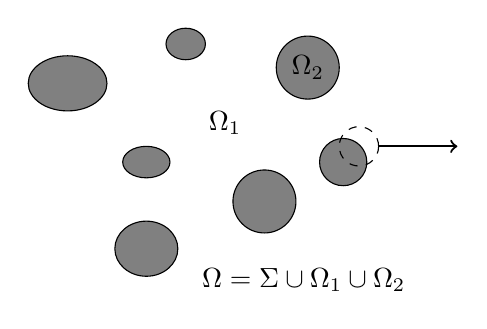
\begin{tikzpicture}
        \foreach \x/\y/\ra/\r in {
        1/3/0.2/0.25,
        2.55/2.7/0.4/0.4,
        0.5/0.4/0.35/0.4,
        2/1/0.4/0.4,
        3/1.5/0.3/0.3,
        0.5/1.5/0.2/0.3,
        -0.5/2.5/0.35/0.5}{
            \draw[fill=gray](\x,\y) ellipse(\r cm and \ra cm);
        }
        \draw[dashed](3.2,1.7)circle(0.25);
        % \draw[thick,->](3.2,1.7)++(0.1767,0.1767)--++(0.4,0.4)--++(1,0);
        \draw[thick,->](3.2,1.7)++(0.25,0)--++(1,0);
        \draw(2.55,2.7)node{$\Omega_2$};
        \draw(1.5,2)node{$\Omega_1$};
        \draw(2.5,0)node{$\Omega = \Sigma \cup \Omega_1 \cup \Omega_2$};
        % \draw(2.5,-1)node{$\Sigma = \sum_\alpha \Sigma_\alpha$};
        % \draw(2.5,-0.5)node{$\Omega_2 = \sum_\alpha \Omega_\alpha$};
    \end{tikzpicture}
    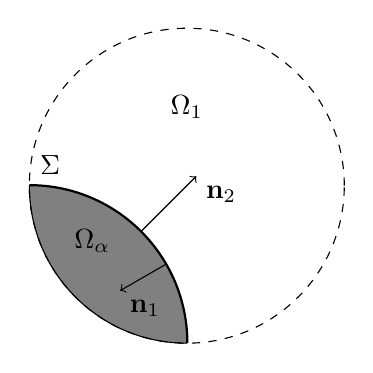
\begin{tikzpicture}%[scale = 0.9]
        \draw[very thick](0:2)arc(0:90:2)node[above right]{$\Sigma$};
        \draw[fill=gray](0:2)arc(0:90:2)arc(180:270:2);
        \draw[dashed](2,2)circle(2);
        \draw[->](1.42,1.42)--++(0.7,0.7)node[below right]{$\textbf{n}_2$};
        \draw[->](1.73,1)--++(-0.577,-0.333)node[below right]{$\textbf{n}_1$};
        \draw(2,3)node{$\Omega_1$};
        \draw(0.8,1.3)node{$\Omega_\alpha$};
    \end{tikzpicture}
    \caption{Scheme of the topology of dispersed two phase flows.}
    \label{fig:Scheme}
\end{figure}
From now on the $k$ indies will refer to either the phase $1$ or $2$, and we drop the time and position arguments in each functions. 
Then, the transport equation of $\chi_k$ can be written as \citep{drew1983mathematical,kataoka1986local,morel2015mathematical},
\begin{equation}
    \pddt \chi_k
    + \textbf{u}_I \cdot \nablabh \chi_k
    = 0,
    \label{eq:dt_chi_k}
\end{equation}
where $\textbf{u}_I$ is the velocity of $\Sigma(t)$.
Besides, it can be shown \citep{tryggvason2011direct,drew1983mathematical,kataoka1986local,bothe2022sharp} that,
\begin{equation}
    \nablabh \chi_k
    = - \delta_I \textbf{n}_k
    \label{eq:grad_chi_k}
\end{equation}
where we have introduced the Interface Indicator Function (IIF) defined as $\delta(\textbf{y}-\textbf{y}_I)$, with $\delta$ being the Dirac-delta function and $\textbf{y}_I$ the position vectors lying on the domain $\Sigma(t)$.
We also define $\textbf{n}_k$ as the outward normal vector of the domain $\Omega_k$.
Taking the gradient of \ref{eq:dt_chi_k} yields the IIF transport equation namely,
\begin{equation}
    \pddt \delta_I
    + \nablabh \cdot \left[(\textbf{u}_I\cdot\textbf{n})\textbf{n} \delta_I\right]
    = \delta_I (\textbf{u}_I\cdot\textbf{n})(\nablabh \cdot\textbf{n})
\end{equation}
As pointed out by \citet{morel2007surface}, it is more convenient to rewrite this equation under the following form,
\begin{equation}
    \pddt \delta_I
    + \nablabh \cdot (\delta_I \textbf{u}_I)
    = \delta_I \nablabhI \cdot \textbf{u}_I.
    \label{eq:dt_delta_I}
\end{equation}
where we introduced the surface divergence operator defined as $\nablabhI \cdot ()= (\textbf{I}-\textbf{nn})\cdot \nablabh \cdot ()$.
Likewise, we can derive an expression for the gradient of $\delta_I$ by taking the gradient of \ref{eq:grad_delta_I} yielding,
\begin{equation}
    % &
    \nablabh\delta_I 
    = \textbf{n} \cdot \nablabh (\textbf{n} \delta_I),
    % &
    % \pddt\delta_I 
    % = - \textbf{n} \cdot \nablabh (\textbf{u}_I  \cdot \textbf{n} \delta_I)
    \label{eq:grad_delta_I}
\end{equation}


Let $f_k(\textbf{y})$ being a volumetric property of the flow solely defined in $\Omega_k(t)$.
Likewise, let $f_I(\textbf{y})$ be an arbitrary surface property defined on $\Sigma(t)$.
Then it is possible to derive the local conservation equations for volumetric and surface quantities \citep{bothe2022sharp,morel2015mathematical,tignol1986modelisation}, using Reynolds transport theorem  and divergence theorem on an arbitrary control volume.
These conservation laws read as, 
\begin{align}
    \label{eq:dt_f_k}
    \pddt f_k
    &= \nablabh \cdot \left(
        \bm{\Phi}_k
        - f_k\textbf{u}_k
        \right)
    + \textbf{S}_k
    & \text{ in } \Omega_k,&\\
    \pddt f_I  
    &= 
    \nablabhI \cdot (\mathbf{\Phi}_{I||} - f_I \textbf{u}_I)
    + \textbf{S}_I
    - \Jump{
        f_k (\textbf{u}_I - \textbf{u}_k)
        + \mathbf{\Phi}_k
     } 
    & \text{ on } \Sigma&
    \label{eq:dt_f_I}
\end{align}
for respectively the volumetric and surface properties.
In \ref{eq:dt_f_I} we introduced the notation $\Jump{\ldots}$ to indicate the sum over both phases, i.e. $\sum_{k=1}^2 [\ldots] \cdot \textbf{n}_k$. 
Where we introduced $\bm{\Phi}_k$ and $\bm{\Phi}_I$ as the non-conservative flux tensor corresponding to $f_k$ and $f_I$. 
The non-conservative flux is often expressed through a constitutive equation depending on the nature of the flow such as the stress tensor for the momentum.
$\textbf{S}_k$ and $\textbf{S}_I$ is defined as the volumetric source term of respectively the phase $k$ and at the interface $\Sigma$.
It is important to notice that \ref{eq:dt_f_k} and \ref{eq:dt_f_I} are solely defined in respectively $\Omega_k$ and $\Sigma$, therefore these equations are referred as local conservation equations.

To generalize these equations over the domain $\Omega$ we follow the formalism of \citet{drew1983mathematical,marle1982macroscopic} and \citet{kataoka1986local} for the volumetric quantities.
Indeed, to any local quantities $f_k$ defined in $\Omega_k$, we assign the field $\chi_k f_k$ which is defined in $\Omega$. 
Similarly, for any local surface quantities $f_I$ defined on $\Sigma$ we assign the field quantity $\delta_I f_I$ defined on $\Omega$. 
Then, multiplying \ref{eq:dt_f_k} and \ref{eq:dt_f_I} by respectively $\chi_k$ and $\delta_I$, and making use of \ref{eq:dt_chi_k} and \ref{eq:dt_delta_I} gives, 
\begin{align}
    \pddt (\chi_k f_k)
    &= \nablabh \cdot (\chi_k \bm{\Phi}_k - \chi_k f_k \textbf{u}_k)
    + \chi_k \textbf{S}_k
    + \delta_I\left[
        \bm{\Phi}_k
        + f_k
        \left(
            \textbf{u}_I
            - \textbf{u}_k
        \right)
    \right]
    \cdot \textbf{n}_k ,
    % & \forall \textbf{y} \in \Omega&
    \label{eq:dt_chi_k_f_k}\\
    \pddt (\delta_If_I)  
    &= 
    \nablabh \cdot (\delta_I \mathbf{\Phi}_{I||} - \delta_I f_I \textbf{u}_I)
    +\delta_I\textbf{S}_I 
    - \delta_I \Jump{
    f_k (\textbf{u}_I - \textbf{u}_k)
    + \mathbf{\Phi}_k
    }.
    \label{eq:dt_delta_I_f_I}
\end{align}
We obtained $k$'s equations defined over the domain $\Omega$ for the bulk quantities, and third global equations for the surface quantities also valid over $\Omega$. 
The transformation of these equations from local to global conservation makes appear a term on the RHS of \ref{eq:dt_chi_k_f_k} representing the interfacial transfer of $f_k$ and $\mathbf{\Phi}_k$, while the surface transport equation did not change fundamentally. 
The set of equations formed by \ref{eq:dt_chi_k_f_k} for $k =1,2$ is commonly known as the \textit{two-fluid} formulation of multiphase flows, to which we add the \textit{jump condition} across the phase given by \ref{eq:dt_delta_I_f_I} \citep{morel2015mathematical,tryggvason2011direct,drew1983mathematical,kataoka1986local}. 
In this work, we prefer to think of those equations as a set of three equations, formed by \ref{eq:dt_chi_k_f_k} for the volumetric conservation equations and \ref{eq:dt_delta_I_f_I} for the surface conservation equations. 

Now that we properly defined the volumetric and surface conservation laws over $\Omega$, let's derive of two phase flows.
We now define any bulk quantity $f$ as $f = \sum_k \chi_k f_k + \delta_I f_I$.
Then adding \ref{eq:dt_chi_k_f_k} for $k=1,2$ and \ref{eq:dt_delta_I_f_I} give the commonly known as the \textit{single-fluid} formulation,
\begin{equation}
    \pddt f
    = \nablabh \cdot (\bm{\Phi} - f \textbf{u})
    + \textbf{S}.
    \label{eq:dt_f}
\end{equation}
Actually, it is more common in the literature to define the bulk quantities as $f = \sum_k \chi_k f_k$ and consider the interfacial terms as source terms as it is often neglected \citep{morel2015mathematical,tryggvason2011direct}. 
Nevertheless, in this work we consider a general case without approximation therefore it is more convenient to think of the bulk quantities as a sum of three phase quantities. 

\subsection{The averaged conservation equations}
\label{sec:avg_def}
In this study, we employ the ensemble average technique to establish the averaged conservation equations. 
This method is just one of several averaging approaches, including the volume average method \citep{jackson1997locally} and time averaging \citep{ishii2010thermo}. 
Despite their differences, all these techniques yield the same set of averaged equations \citep{jackson1997locally,zhang1997momentum}.
In the following we recall some properties of the ensemble average operator. 
Let, $P(\FF)$ be the probability density function that describes the probability of finding the flow in the configuration $\FF$. 
We note $d\PP = P(\FF) d\FF$ the probable number of flows located in the incremental region of the phase space $d\FF$ around the point $\FF$. 
It follows from this definition, that the ensemble average of an arbitrary local property $f^0(\textbf{x},t;\FF)$ defined on the whole space $\Omega$, is,
\begin{equation}
    f(\textbf{x},t)
    = \avg{f^0}(\textbf{x},t)
    =\int f^0(\textbf{x},t;\FF) d\mathscr{P}. 
    \label{eq:avg}
\end{equation}  
Note that we dropped the super script $^0$ on $f(\textbf{x},t)$ to indicate that this is an averaged quantity. 
The macroscopic variables are averaged over all $\FF$, and therefore depend only on $\textbf{x}$ and $t$.
Thus, we omit the arguments of the averaged fields, as this notation eliminates any potential ambiguity. 
The ensemble average quantities are assumed to satisfy the following properties \citep{drew1983mathematical}
\begin{align}
    \label{eq:avg_properties}
    \avg{f^0+h^0} &= f+h, \\ 
    \avg{\avg{f^0}h^0} &= fh, \\
    \avg{\pddt f^0} 
    &= \pddt f, \\ 
    \avg{\grad f^0}
    &= \grad f. 
\end{align}
were $f$ and $h$ are two arbitrary Eulerian fields. 
The first two relations are called the Reynolds' rules, the third one is the Leibniz' rule and the last one, is the Gauss' rule \citep{drew1983mathematical}.
Additionally, for any phase quantity defined in $\Omega_k$ we introduce the definition, 
\begin{equation}
    \phi_k f_k (\textbf{x},t) = \avg{\chi_k f_k^0},
    \label{eq:1_avg}
\end{equation}
where $\phi_k(\textbf{x},t) = \avg{\chi_k}$ is the volume fraction of the phase $k$.
And $f_k$ is the average of the field $f_k^0$ conditioned on the presence of the phase $k$ in the configuration $\FF$ at $\textbf{x}$ and time $t$.
Equally, for interface quantities we have 
\begin{equation}
    \phi_I f_I (\textbf{x},t) = \avg{\delta_I f_I^0},
\end{equation}
with $\phi_I = \avg{\delta_I}$ the interfacial area concentration function. 
Here, $f_I$ is the average of $f^0_I$ conditioned on the presence of an interface in the configuration $\FF$ at $\textbf{x}$ and time $t$. 
Additionally, we define the field of fluctuation of a given quantity around its mean as,
\begin{align}
    f'(\textbf{x},t,\FF) = f^0(\textbf{x},t,\FF) - f(\textbf{x},t).
    \label{eq:def_fluctu}
\end{align}
This relation applies to phase averaged quantities such that $f'_k = f^0_k - f_k$ and $f'_I = f^0_I - f_I$. 


Applying the ensemble average on \ref{eq:dt_chi_k_f_k} and \ref{eq:dt_delta_I_f_I} and considering the properties from \ref{eq:avg_properties} to \ref{eq:def_fluctu}, yields the general form of the averaged equations of multiphase flows, namely,
\begin{align}
    \pddt (\phi_k f_k)
    +\div (\phi_k f_k \textbf{u}_k - \mathbf{\Phi}_k^\text{eq})
    &= 
    \phi_k s_k
    + \avg{\delta_I\left[
        \mathbf{\Phi}_k^0
        + f_k^0
        \left(
            \textbf{u}_I^0
            - \textbf{u}_k^0
        \right)
    \right]
    \cdot \textbf{n}_k} ,
    \label{eq:avg_dt_chi_f}\\
    \pddt (\phi_I f_I)
    +\div (\phi_I f_I \textbf{u}_I- \mathbf{\Phi}_{I}^\text{eq})
    &= 
    \phi_I s_I
    - \avg{\delta_I 
    \Jump{
    f_k^0 (\textbf{u}_I^0 - \textbf{u}_k^0)
    + \mathbf{\Phi}_k^0
    } 
     },
    \label{eq:avg_dt_delta_f}
\end{align}
with, 
\begin{align*}
    \mathbf{\Phi}_k^\text{eq}
    = \avg{\chi_k f_k' \textbf{u}_k'}
    - \phi_k \bm\Phi_k,
    &&
    \mathbf{\Phi}_{I}^\text{eq}
    = \avg{\delta_I f_I' \textbf{u}_I'}
    - \phi_I \bm\Phi_I. 
\end{align*}
These equations are to be solved for the averaged field $\phi_k,\phi_I,f_k$ and $f_I$ with a complementary equation of volume conservation, i.e. $\phi_f+\phi_d+\phi_I = 1$.
The main differences between these equations and their microscale counterparts (\ref{eq:dt_f_k} and \ref{eq:dt_f_I}) are:
(1) The unknowns are now averaged quantities,
(2) Factors $\phi_k$ and $\phi_I$ are introduced in front of all the terms, and
(3) The additional terms $\avg{\chi_k f_k' \textbf{u}_k'}$ and $\avg{\delta_I f_I' \textbf{u}_I'}$ appear, representing the covariance between the conserved quantity ($f_k$ or $f_I$) and the local velocities.  
For a complete understanding, we derived the mass, momentum, and energy averaged equations in \ref{ap:two-fluid_model}. 
These are derived considering the simplifying hypothesis exposed in \ref{ap:hypothesis}. 
In addition, \ref{ap:two-fluid_model} presents how to derive the secondary averaged equations of the averaged energy $E_k$, i.e. the equation for the mean internal energy $e_k$, the pseudo turbulent energy $k_k = \frac{1}{2\phi_k}\avg{\chi_k (u'_k)^2}$, and the averaged kinetic energy $(u_k)^2/2$.  


It is important to highlight that the two-fluid model fails to adequately distinguish between the two phases, as evidenced by the \textit{symmetry} $k = 1$ and $2$ in the aforementioned equations. This symmetry does not hold physically because the dispersed phase possesses a distinct topological nature compared to the continuous phase. 
More importantly, in a dispersed two-phase flow system the closure terms are expressed as a function of the Lagrangian properties of the particles whereas this system of equation provides us with continuously averaged quantities. 
Specifically, the mean drag force or torque term in the averaged momentum equation is expressed as a function of the center of mass linear and angular velocity  of the particles. 
Whereas this system of equation provides us with the phase averaged velocity of the whole phase not with no consideration for the particles properties.  
Therefore, in the subsequent section, we will introduce a kinetic model specifically devoted to the dispersed phase. 
As illustrated below, the equations governing the dispersed phase are more comprehensive as they bear a resemblance to the equations governing a single particle.



\section{Lagrangian equations for the dispersed phase}
\label{sec:Lagrangian}

In this section, we present a Lagrangian-based model capable of describing the dispersed phase with an arbitrary order of accuracy.

\subsection{Fundamental properties}

At this stage, we define some fundamental properties associated to each particle labeled $\alpha$.
Following the strategy of \citet{lhuillier2009rheology,lhuillier1992volume,zaepffel2011modelisation} and \citet[Chapter 2]{morel2015mathematical}
we define the mass $m_\alpha$, position of center of mass $\mathbf{x}_\alpha$, and the momentum $\textbf{p}_\alpha$ of the particle $\alpha$, as
\begin{align}
    m_\alpha(t,\FF)
    = \intO{ \rho_d  }, 
    &&
    \textbf{x}_\alpha(t,\FF)
    = \frac{1}{m_\alpha(t,\FF) }\intO{ \rho_d \textbf{x} }, 
    &&\textbf{p}_\alpha(t,\FF) 
    = \intO{ \rho_d \textbf{u}_d^0 }.
    \label{eq:mass_pos}
    % \label{eq:momentum_energy}
\end{align}
$\Omega_\alpha(t,\FF)$ is the time-dependent domain occupied by the particle $\alpha$ (see \ref{fig:Scheme}). 
Subsequently, we define the velocity of the particle center of mass as
\begin{equation*}
\textbf{u}_\alpha = \frac{d \textbf{x}_\alpha}{dt}.
\end{equation*}
Replacing $\textbf{x}_\alpha$ by its definition (\ref{eq:mass_pos}) we obtain
\begin{equation*}
    \textbf{u}_\alpha = \frac{1}{m_\alpha}
    \frac{d}{dt} 
    \left(
        \intO{ \rho_d \textbf{x} }
    \right)
    - \frac{1}{m_\alpha^2} \frac{d}{dt} \left(\intO{ \rho_d } \right)
    \intO{ \rho_d \textbf{x} }.
\end{equation*}
%\tb{ A finaliser
Using the Reynolds transport theorem (\ref{eq:reynolds_transport}) for both terms in parentheses and making use of the conservation of mass (\ref{eq:dt_rho}) and the definition of $\textbf{x}_\alpha(t,\FF)$ in the last term, gives
\begin{equation}
    \textbf{u}_\alpha = 
    \frac{1}{m_\alpha}\intO{ \left[
        \pddt (\textbf{x}\rho_d ) + \div\left(\textbf{u}_d \textbf{x} \rho_d\right) 
    \right]} \\
    + \frac{1}{m_\alpha}\intS{ \textbf{x} \rho_d(\textbf{u}_I   - \textbf{u}_d) \cdot \textbf{n}_d }
    -  \frac{\textbf{x}_\alpha}{m_\alpha}    \intS{ \rho_d(\textbf{u}_I   - \textbf{u}_d) \cdot \textbf{n}_d }
\end{equation}
Then by considering the mass conservation for the first term and noticing that $\grad \textbf{x} = \bm\delta$, for the second term gives, 
\begin{equation}
    \textbf{u}_\alpha(t,\FF) = \frac{1}{m_\alpha(t,\FF)} \left(
        \textbf{p}_\alpha(t,\FF)
        +  \intS{\rho_d \textbf{r} (\textbf{u}_I^0 - \textbf{u}_d^0)\cdot \textbf{n}_d }
        \right),
        \label{eq:dt_y_alpha}
\end{equation}
where $\textbf{r}(\textbf{x},t) = \textbf{x} - \textbf{x}_\alpha(t)$. 
In \ref{eq:dt_y_alpha}, it can be observed that the first component of the velocity represents the linear momentum divided by the mass of the particle. 
This corresponds to the mass-averaged velocity over the volume of the particle.
The second term in \ref{eq:dt_y_alpha} arises from the contribution of anisotropic mass transfer across the surface of the particle. 
This mass transfer leads to the motion of the particle's center of mass, thereby contributing to the total velocity.
To illustrate this concept, let us consider a fixed drop with no momentum lying over a very hot plate.
In this scenario, we assume that the plate is sufficiently hot to induce evaporation, specifically on the bottom portion of the drop.
Hence, under the effect of an anisotropic evaporation flux one may expect the second term to be non-negligible.
Consequently, the center of mass of the drop has a non-zero velocity in the opposite direction of the plate, even though the momentum is assumed to be zero.
Note that \ref{eq:dt_y_alpha} generalized usual expression of the center of mass velocity whom neglect the second term.
In the following, for the sake of brevity we discard the dependency on $t$ and $\FF$ on the notations for all Lagrangian quantities denoted by the subscript $_\alpha$ and in particular $\Gamma_\alpha$ and $\Omega_\alpha$.
Nevertheless, the reader must understand that all Lagrangian quantities and integration domains subscribed by $_\alpha$ are time and configuration-dependent. 

The particle's internal relative motions or the \textit{inner velocity} is given by $\textbf{w}_d^0 = \textbf{u}_d^0 - \textbf{u}_\alpha$. 
Substituting the inner velocity in the momentum definition (\ref{eq:mass_pos}) yields
\begin{equation}
    \label{eq:momentum_definition_1}
    \textbf{p}_\alpha
    = m_\alpha \textbf{u}_\alpha
    + \int_{\Omega_\alpha} \rho_d \textbf{w}_d^0 d\Omega.
\end{equation}
Alternatively, from \eqref{eq:dt_y_alpha}, we obtain,
\begin{equation}
    \textbf{p}_\alpha
    =  m_\alpha \textbf{u}_\alpha
    - \int_{\Gamma_\alpha} \rho_d\textbf{r}(\textbf{u}_I^0 - \textbf{u}_d^0)\cdot \textbf{n}_d d\Sigma
    \label{eq:momentum_definition}
\end{equation}
Therefore, the momentum of a particle can be seen as a sum of the mean velocity plus the integral of the fluctuation (\ref{eq:momentum_definition_1}), with the latter being equivalent to minus the first moment of mass transfer term (\ref{eq:momentum_definition}).
Indeed, by identification we obtain : $\intO{ \rho_d \textbf{w}_d^0 } = - \intS{  \rho_d\textbf{r} (\textbf{u}_I^0 - \textbf{u}_d^0)\cdot \textbf{n}_d }$. 
Hence, the internal velocity fluctuations within a fluid particle do not contribute to the total linear momentum $\textbf{p}_\alpha$, as long as the anisotropic mass transfer is negligible.  
Only within this simplified context we can consider the classic relation $\textbf{p}_\alpha = m_\alpha \textbf{u}_\alpha$. 

\subsection{Conservation laws}

We assign to a particle indexed, $\alpha$, occupying the domain $\Omega_\alpha$ (see \ref{fig:Scheme}) an arbitrary Lagrangian property $q_\alpha$ defined by $q_\alpha  = \intO{ f_d^0}$.
Similarly, we define $q_{I\alpha} = \intS{ f_I^0}$ as an integrated surface property of the particle $\alpha$.

\subsubsection{Inside the volume}
To describe the evolution of any arbitrary Lagrangian quantity $q_\alpha$, we need to establish its time derivative.
Since $q_\alpha$ is an integral quantity with a time-dependent domain of integration, we apply the general Reynolds transport theorem for volume integral which gives for material domains (here the droplet volume),
\begin{equation}
    \ddt  \intO{f_d^0}
    = \intO{\left[ \pddt f_d^0 + \div\left(f_d^0\textbf{u}_d^0\right) \right]}\\
    + \intS{ f_d^0 (\textbf{u}_I^0-\textbf{u}_d^0)\cdot \textbf{n}_d }.
    \label{eq:reynolds_transport}
\end{equation}
By substituting the integrand of the first integral on the right-hand side (RHS) with \ref{eq:dt_f_k} we obtain the conservation law of the quantity $q_\alpha$, namely,  
\begin{equation}
    \ddt{q_\alpha}
    = \intO{ s_d^0 }
    + \intS{ \left[
        f_d^0 (\textbf{u}_I^0-\textbf{u}_d^0) 
        + \mathbf{\Phi}_d^0 
        \right] \cdot \textbf{n}_d }.
    \label{eq:dt_q_alpha}
\end{equation}
In \ref{eq:dt_q_alpha} we used the Gauss divergence theorem to show that
\begin{equation}
    \intO{\div \mathbf{\Phi}_d^0} = \intS{\mathbf{\Phi}_d^0 \cdot \textbf{n}_d}.
\end{equation}
The first term on the right-hand side of \ref{eq:dt_q_alpha} accounts for the total contribution of the source term $s_d^0$ to the particle $\alpha$,
while the second term is the surface integration of the exchange terms, which includes the phase transfer flux $f_d^0 (\textbf{u}_I^0-\textbf{u}_d^0)$ and the diffusive flux $\mathbf{\Phi}_d^0$. 


Let us consider the specific case of the momentum balance, i.e. $q_\alpha = \textbf{p}_\alpha$.
In this situation, \ref{eq:dt_q_alpha} reads
\begin{equation}
    \ddt  \textbf{p}_\alpha
    = \intO{ \rho_d\textbf{g} }
    + \intS{ 
        \left[
        f_d^0 (\textbf{u}_I^0-\textbf{u}_d^0)
         + \bm{\sigma}_d^0%\cdot\textbf{n}_d  
        %+ \mathbf{\Phi}_d^0 
        \right] 
        \cdot \textbf{n}_d },
\end{equation}
% first term reads as $\intO{ \rho_d\textbf{g} }$ 
The first term on the right-hand side represents the total weight acting on the particle $\alpha$, 
the second term represents the total source of momentum due to phase transfer, and it is expressed as, $\intS{ \rho_d \textbf{u}_d^0 (\textbf{u}_I^0-\textbf{u}_d^0)\cdot\textbf{n}_d }$,
and the last term $\intS{ \bm{\sigma}_d^0\cdot\textbf{n}_d }$, represents the resultant of the hydrodynamic forces acting on the surface of the particle.
It is important to notice that under this form, the exchange terms are expressed as integrals of dispersed phase fields denoted by the subscript $_d$.
Nevertheless, depending on the nature of the dispersed phase, these fields may not always be defined.
For rigid particles the stress within the particle $\bm{\sigma}_d^0$ is indeterminate \citep{guazzelli2011}.  
Hence, our objective is to express these exchange terms, in terms of the continuous phase field quantities instead of the dispersed phase fields, i.e. in terms of $\mathbf{\Phi}_f^0$ and $\textbf{u}_f^0$ rather than $\mathbf{\Phi}_d^0$ and $\textbf{u}_d^0$. 

\subsubsection{On the interfaces}
To address this issue in a general manner, let us derive the conservation equation for the integrated surface property $q_{I\alpha} = \intS{f_I^0}$.
To differentiate time-varying surface integrals within time, we make use of the general Leibniz rule, which states that for an arbitrary function $f_I^0$ defined on $\Gamma(t)$ we have the relation \citep{nadim1996concise}
\begin{equation}
    \ddt  \intS{f_I^0 }
    = \intS{ \left[
        \pddt f_I^0
        +   \gradI \cdot (\textbf{u}_I^0f_I^0)
    \right]}.
    \label{eq:surface_derivative}
\end{equation}
Substituting the right-hand side terms of \ref{eq:surface_derivative} with \ref{eq:dt_f_I}, gives,
\begin{equation}
    \ddt  q_{I\alpha}
    = \intS{ 
        s_I^0
    }
    - \intS{
 \Jump{
        f_k^0 (\textbf{u}_I^0 - \textbf{u}_k^0)
        + \mathbf{\Phi}_k^0
    }
    }.
    \label{eq:dt_q_I_alpha}
\end{equation}
We have used the surface divergence theorem applied to closed surfaces \citep{nadim1996concise}, it reads
\begin{equation}
    \intS{\gradI F}
    = 
    \intS{ F \textbf{n} (\div \textbf{n})},
    \label{eq:gauss_surface}
\end{equation} 
where $F$ is an arbitrary field.
This theorem demonstrates that any surface property parallel to the tangential plane of $\Gamma$, such as $\bm\Phi_{I||}$, satisfies the relation $\intS{\divI \bm\Phi_{I||}^0}
= 0$.
This explains why $\bm\Phi_{I||}$ does not appear in \ref{eq:dt_q_I_alpha}. 
\ref{eq:surface_derivative} can be interpreted as the conservation equation for the integrated surface property $f_I^0$, or as the jump condition of the $f^0_k$ integrated on the droplet surface. 
As discussed above we wish to get rid of $\mathbf{\Phi}_d^0$ in \ref{eq:dt_q_alpha}. 
To achieve this, we treat the particle's volume and surface as a unified entity and derive a conservation equation for $q_\alpha^\text{tot} = q_\alpha + q_{I\alpha}$. 
By summing \ref{eq:dt_q_alpha} and \ref{eq:dt_q_I_alpha} we directly obtain 
\begin{equation}
    \ddt  q_\alpha^\text{tot}
    = 
    \intO{ s_d^0 }
    + \intS{ s_I^0 }
    + \intS{ \left[
        f_f^0 (\textbf{u}_I^0-\textbf{u}_f^0) 
        + \mathbf{\Phi}_f^0 
        \right] \cdot \textbf{n}_d }. 
    \label{eq:dt_q_alpha_tot}
\end{equation}
This equation is the general form of the linear conservation law for the quantity $q_\alpha^\text{tot}$.
It applies to any particle immersed into a continuous phase following the local conservation, \ref{eq:dt_f_k} and \ref{eq:dt_f_I}.
We refer to this equation as the zeroth-order conservation equation or the linear conservation law for the particle $\alpha$.

We would like to highlight that due to the consideration of closed surface, the diffusive flux $\mathbf{\Phi}_{I||}^0$, plays no role at all in \ref{eq:dt_q_alpha_tot}.
Therefore, in the case of the linear momentum conservation law, the contribution of the momentum diffusive flux $\bm\sigma_{I||}^0$ exposed in \ref{eq:dt_rhoIu_I}, will not contribute to the momentum balance of a particle, and we obtain the relation 
\begin{equation}
    \ddt  \textbf{p}_\alpha^\text{tot}
    = 
    \intO{ \rho_d^0\textbf{g} }
    + \intS{ \rho_I^0\textbf{g} }
    + \intS{ 
        \left[
        f_d^0 (\textbf{u}_I^0-\textbf{u}_f^0)
        + \bm{\sigma}_f^0
        \right] 
        \cdot \textbf{n}_d }. 
\end{equation}
In this case, note that $\textbf{p}_\alpha^\text{tot} = \intO{\rho^0_d \textbf{u}_d^0}+\intS{\rho^0_I \textbf{u}_I^0}$ is the momentum of the particle's volume and surface. 
The latter might be negligible if the interface has a negligible weight. 
As a consequence, even in the presence of local Marangoni forces or surface viscous stresses (see \ref{eq:surface_fluxes}), the resultant of the surface diffusive fluxes would still cancel out in the linear momentum balance.
This fact has already been demonstrated by \citet{hesla1993note} who showed that the surface tension force does not contribute to the linear and angular momentum balance. 
Here, we have provided the general proof that the interfacial diffusive flux $\mathbf{\Phi}_{I||}^0$, which is present at the local scale according to \ref{eq:dt_f_I}, does not contribute to the zeroth-order conservation law of a particle with a closed surface.

For completeness, we exposed in \ref{ap:particles_eq} a clear derivation of the mass, momentum and total energy equations for a single particle.
The derivation takes place using the same hypothesis as it is exposed in \ref{ap:hypothesis}.
Especially, it is shown that the integration of the kinetic energy jump condition corresponds to the Lagrangian derivative of the particle surface, see \ref{eq:int_u_I2}. 

\subsection{Higher moment equations}

Because $f_d^0$ and $f_I^0$ are not always constant over the volumes and surfaces of the particles, it is interesting to introduce in the first place, the first moment of the quantities $f_d^0$ and $f_I^0$. 
They are defined as
\begin{align}
    &\textbf{Q}_\alpha 
    = \intO{ \textbf{r} f_d^0 },
    &\text{and}&
    &\textbf{Q}_{I\alpha}
    = \intS{ \textbf{r} f_I^0 },
    \label{eq:first_moment_definition}
\end{align}
where we recall that $\textbf{r} = \textbf{x} - \textbf{x}_\alpha$ is the distance between any point inside $\Omega_\alpha$ or $\Gamma_\alpha$, to the center of mass of the particle $\alpha$.
It is then possible to differentiate these moments with respect to time to obtain their conservation laws.
We use the Reynolds transport theorem (\ref{eq:reynolds_transport}) to describe the evolution of $\textbf{Q}_\alpha$ within time. 
It gives, 
\begin{equation*}
    \frac{d}{dt} \textbf{Q}_\alpha
      =  \intO{\left[
        \pddt(  f_d^0\textbf{r})
        + \div \left(  f_d^0 \textbf{r}\textbf{u}_d^0\right)
    \right]} 
    + \intS{  f_d^0 \textbf{r}  (\textbf{u}_I^0-\textbf{u}_d^0)\cdot \textbf{n}_d}
\end{equation*}
The first term on the right-hand side may be rewritten as
\begin{equation*}
\intO{ \left[
        \pddt(\textbf{r}  f_d^0)+ \div \left( \textbf{u}_d^0 \textbf{r} f^0_d\right) 
    \right]}
    = \intO{\textbf{r}\left[
        \pddt f_d^0
        + \div \left(f_d^0 \textbf{u}_d^0\right)
    \right] }
    + \intO{ f_d^0 \left[
        \pddt \textbf{r}
        +(\textbf{u}_d^0 \cdot \grad) \textbf{r}
    \right]}
\end{equation*}
Using \ref{eq:dt_f_k} for the first integral on the right-hand side, and considering the relation,
$  \pddt \textbf{r}
+ (\textbf{u}_d^0 \cdot \grad) \textbf{r}
= - \frac{d}{dt} \textbf{y}_\alpha  + \textbf{u}_d^0 
= \textbf{w}_d^0$,
for the second integral yields 
\begin{align}
    \frac{d}{dt} \textbf{Q}_\alpha
    % &= \intO{\textbf{r} \left[
    %      s_d^0  +  \div \bm\Phi_d^0
    % \right]}
    % +\intO{f_d^0  \textbf{w}_d }
    % + \int_{\Gamma_\alpha} \textbf{r}  f_d^0 (\textbf{u}_I^0-\textbf{u}_d^0)\cdot \textbf{n}_d  d\Sigma,\\
    = \intO{\left( 
        \textbf{r} s_d^0  
        + f_d^0  \textbf{w}_d 
        - \bm\Phi_d^0
    \right) }
    + \int_{\Gamma_\alpha} \textbf{r} \left[
        \bm\Phi_d^0
        + f_d^0 (\textbf{u}_I^0-\textbf{u}_d^0)
    \right]\cdot \textbf{n}_d  d\Sigma.
    \label{eq:dt_Q_alpha}
\end{align}
Where we have used the relation $\intO{\textbf{r}  \div \bm\Phi_d^0 }
= \intS{ \textbf{r} \bm\Phi_d^0 \cdot \textbf{n}_d }
- \intO{ \bm\Phi_d^0 }$. 
\ref{eq:dt_Q_alpha} is the first order moment conservation equation for the particle $\alpha$. 
Following the same procedure, and making use of \ref{eq:surface_derivative}, \ref{eq:gauss_surface} and \ref{eq:dt_f_I}, one can equally show that 
\begin{align}
    \ddt {\textbf{Q}_{I\alpha}}
    &= \intS{ \left(
        \textbf{r}s_I^0
        + f_I^0 \textbf{w}_I^0
        - \mathbf{\Phi}_{I||}^0
    \right) }
    - \intS{\textbf{r} 
    \Jump{\mathbf{\Phi}_k^0
        + f_k^0 (\textbf{u}_I^0 - \textbf{u}_k^0)
    }
    },
    \label{eq:dt_Q_I_alpha}
\end{align}
where $\textbf{w}_I^0 = \textbf{u}_{I||}^0 - \textbf{u}_\alpha$.
In \ref{eq:dt_Q_alpha}, we recognize the first moment of the source term $s_d^0$, the first moment of the diffusive flux term $\bm\Phi_d^0\cdot\textbf{n}_d$ and the first moment of phase exchange term, $f_d^0 (\textbf{u}_I^0-\textbf{u}_d^0)\cdot\textbf{n}_d$. 
Additionally, two supplementary terms appear in \ref{eq:dt_Q_alpha}, namely: the integral of the diffusive flux $\bm\Phi_d^0$, and a term related to the fluctuation of the internal velocity $f_d^0 \textbf{w}_d^0$.
Similar observations can be made for the first moment of surface equation \ref{eq:dt_Q_I_alpha}, as it shares similarities with \ref{eq:dt_Q_alpha}. 
In particular, it is worth noting the presence of the surface diffusive flux $\mathbf{\Phi}_{I||}^0$ in \ref{eq:dt_Q_I_alpha}.
This term will be further discussed in the following. 

For similar reason than the linear conservation equations, we sum \ref{eq:dt_Q_alpha} and \ref{eq:dt_Q_I_alpha} to expresses the conservation equation of the total first moment $\textbf{Q}_\alpha^\text{tot} = \textbf{Q}_\alpha + \textbf{Q}_{I\alpha}$, this yields 
\begin{multline}
    \ddt {\textbf{Q}_\alpha^\text{tot}}
    = \intO{ \left(
        \textbf{r} s_d^0         
        + f_d^0  \textbf{w}_d^0 
        - \mathbf{\Phi}_d^0
    \right) }
    + \intS{ \left(
        \textbf{r}s_I^0
        + f_I^0 \textbf{w}_I^0
        - \mathbf{\Phi}_{I||}^0
    \right) }
    + \intS{ \textbf{r} \left[
        \mathbf{\Phi}_f^0
        + f_f^0 (\textbf{u}_I^0-\textbf{u}_f^0)
    \right]\cdot \textbf{n}_d  }. 
    \label{eq:dt_Q_alpha_tot}
\end{multline}
Likewise, conservation laws can be derived for the $n^{th}$ order moments of volume and surface, i.e. for
\begin{align}
    \textbf{Q}_{\alpha n}
    = \intO{
         \underbrace{\textbf{rr}\ldots \textbf{rr}}_{n\text{ times}}
        f_d^0 },
        && \text{and} &&
    \textbf{Q}_{I\alpha n}
    = \intS{
         \underbrace{\textbf{rr}\ldots \textbf{rr}}_{n\text{ times}}
    f_I^0 },
    \label{eq:Q_n_definition}
\end{align} 
respectively. 
It can be shown that the derivative with time of $\textbf{Q}_{\alpha n}$ and $\textbf{Q}_{I\alpha n}$ do not involve any additional terms than in \ref{eq:dt_Q_alpha} and \ref{eq:dt_Q_I_alpha}, but rather just the $n^{th}$ order moments of the already presented terms.
We provide the full derivation of $\ddt{ \textbf{Q}_{\alpha n}}$ in \ref{ap:Moments_equations}.
In short, these higher order moments describe the distributions of the local quantities $f_d^0$ and $f_I^0$ inside the domain $\Omega_\alpha$ and $\Gamma_\alpha$, respectively.
Consequently, an infinite number of moments would be theoretically necessary to recover the fields $f_d^0$ and $f_I^0$ within $\Omega_\alpha$ and $\Gamma_\alpha$. 
Thus, one can reach an arbitrary order of accuracy upon the knowledge of an arbitrary number of moments for a given quantity.  

\subsection{Discussion}

To gain physical insight into the meaning of the first and higher moment equations, we now consider the case of mass and momentum conservation laws for a particle of arbitrary shape. 
For ease of understanding, we adopt the simplifying hypotheses presented in \ref{ap:hypothesis}. 
This implies that we consider no mass transfer across phases and no surface properties except for surface tension forces.

Following \ref{eq:Q_n_definition} we define the second-order moment of mass and the first-order moment of momentum as respectively,
\begin{equation}
    \textbf{M}_\alpha 
    = \intO{ \rho_d \textbf{r} \textbf{r} }
    \;\;\;\text{and}\;\;\;
    \textbf{P}_\alpha 
    = \intO{ \rho_d \textbf{r} \textbf{u}_d^0 }.
    \label{eq:first_moment_of_momentum_def}
\end{equation}
Note that $\textbf{M}_\alpha$ is analogous to the inertia tensor $\textbf{I}_\alpha$ in solid mechanics, both are related through the expression $\textbf{I}_\alpha = \bm\delta : \textbf{M}_\alpha - \textbf{M}_\alpha$.
For a constant density, the tensor $\textbf{M}_\alpha$ describes the second moment of the volume distribution around the particle center of mass.
Likewise, the tensor $\textbf{P}_\alpha$ describes the first moment of the velocity distribution within the particle volume. 
To provide a clearer physical interpretation of the moment of momentum tensor, we decompose $\textbf{P}_\alpha$ into two distinct parts. 
Namely, 
$\textbf{P}_\alpha = \textbf{S}_\alpha+\textbf{T}_\alpha$, where $\textbf{S}_\alpha$ represents the symmetric part and $\textbf{T}_\alpha$ is the antisymmetric part of $\textbf{P}_\alpha$.
Then, the tensors $\textbf{S}_\alpha$ and $\textbf{T}_\alpha$ correspond respectively to the stretching and angular momentum of the particle $\alpha$. 
The tensor $\textbf{S}_\alpha$ quantifies how fast and in which direction the particle gets elongated or flattened, in other words it represents the mean rate of deformation experienced by the particle.
The tensor $\textbf{T}_\alpha$ is related to the angular momentum of the particle denoted by the pseudo vector $\bm\mu_\alpha = \intO{ \rho_d \textbf{r} \times \textbf{u}_d^0 }$. 
Indeed, both  $\textbf{T}_\alpha$ and $\bm{\mu}_\alpha$ represent the angular momentum and are related through $(\bm{\mu}_\alpha)_i = \epsilon_{ijk} (\textbf{P}_\alpha)_{jk}= \epsilon_{ijk} (\textbf{T}_\alpha)_{jk}$, where $\bm\epsilon$ is the third order alternating unit tensor or Levi-Cita tensor. 
Lastly, we also introduce the scalar $M_\alpha =\frac{1}{3}\bm\delta : \textbf{P}_\alpha = \frac{1}{3}\intO{ \rho_d \textbf{r} \cdot \textbf{u}_d^0 }.$, which quantifies the rate at which the particle is being compressed or expanded.
To better explain the implication of these quantities on the particle kinematics we provide in \ref{eq:scheme}, three schemes representing possible inner velocity fields with their corresponding value of the moment of momentum tensor.
Note that in \ref{eq:scheme} we explicit
\begin{figure}[h!]
    \centering
    \hfill
    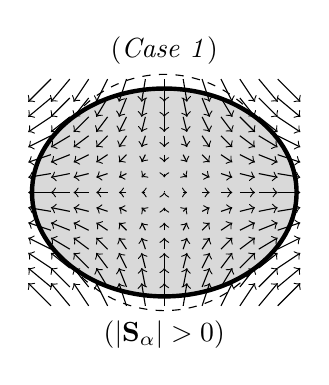
\begin{tikzpicture}[ultra thick,scale=0.6]
        \def\nRows{6}
        \def\nCols{6}
        \draw[dashed,thin] (0,0)circle(2.5);
        \draw[fill=gray!30] (0,0)ellipse(2.8 and 2.2);
        \foreach \x in {-\nRows,...,\nRows} {
            \foreach \y in {-\nCols,...,\nCols} {
                \pgfmathsetmacro\distance{veclen(\x*0.4, \y*0.4)};
                \pgfmathparse{\distance < 2.45 ? "blue" : "white"}
                \edef\colour{\pgfmathresult};
                \ifthenelse{\equal{\colour}{blue}}{                    
                    \draw[thin,->](\x*0.4,\y*0.4)--++(0.08*\x,-0.08*\y);
                }
            }
        }
        \node (txt) at (0,3){(\textit{Case 1})};
        \node (txt) at (0,-3){($|\textbf{S}_\alpha| > 0$)};
    \end{tikzpicture}
     \hfill
    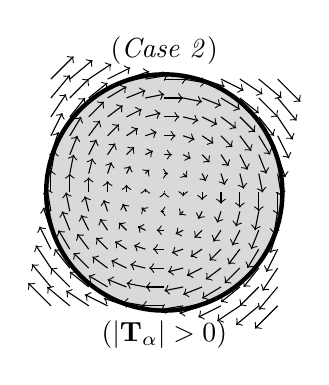
\begin{tikzpicture}[ultra thick,scale=0.6]
        \def\nRows{6}
        \def\nCols{6}
        \draw[fill=gray!30] (0,0)circle(2.5);
        \foreach \x in {-\nRows,...,\nRows} {
            \foreach \y in {-\nCols,...,\nCols} {
                \pgfmathsetmacro\distance{veclen(\x*0.4, \y*0.4)};
                \pgfmathparse{\distance < 2.5 ? "blue" : "white"}
                \edef\colour{\pgfmathresult};
                \ifthenelse{\equal{\colour}{blue}}{                    
                    \draw[thin,->](\x*0.4,\y*0.4)--++(0.08*\y,-0.08*\x);
                }
            }
        }
        \node (txt) at (0,3){(\textit{Case 2})};
        \node (txt) at (0,-3){($|\textbf{T}_\alpha| > 0$)};
    \end{tikzpicture}
    \hfill
    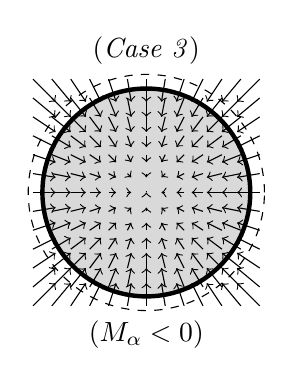
\begin{tikzpicture}[ultra thick,scale=0.6]
        \def\nRows{6}
        \def\nCols{6}
        \draw[dashed,thin] (0,0)circle(2.5);
        \draw[fill=gray!30] (0,0)circle(2.2);
        \foreach \x in {-\nRows,...,\nRows} {
            \foreach \y in {-\nCols,...,\nCols} {
                \pgfmathsetmacro\distance{veclen(\x*0.4, \y*0.4)};
                \pgfmathparse{\distance < 2.3 ? "blue" : "white"}
                \edef\colour{\pgfmathresult};
                \ifthenelse{\equal{\colour}{blue}}{                    
                    \draw[thin,->](\x*0.4,\y*0.4)--++(-0.08*\x,-0.08*\y);
                }
            }
        }
        \node (txt) at (0,3){(\textit{Case 3})};
        \node (txt) at (0,-3){($M_\alpha < 0$)};
    \end{tikzpicture}
    \hfill
    \caption{Graphical representation of the inner kinematics of an arbitrary particle under three scenarios. 
        The arrows represent the velocity field inside the particle, $\textbf{w}_d^0$, with the corresponding value of the moment of momentum tensor indicated below. 
        The operator $|\ldots|$ refers to the norm of the tensors. 
        According to the inner velocity field:
        (\textit{Case 1}) The particle experiences a mean rate of deformation, resulting in non-zero stretching of momentum along the principal axis of deformation;
        (\textit{Case 2}) The particle is rotating, leading to a non-zero angular momentum vector in the direction of rotation;
        (\textit{Case 3}) The particle undergoes compression, resulting in a negative trace of the moment of momentum.
    }
    \label{eq:scheme}
\end{figure}

Injecting, $f_d^0 = \rho_d$ in the second-order moment equation (derived in \ref{ap:Moments_equations}) we obtain :
\begin{equation}
    \ddt {\textbf{M}_\alpha}=2\textbf{S}_\alpha. 
    \label{eq:dt_M_alpha}
\end{equation}
which is the second-order moment of mass conservation equation. 
From \ref{eq:dt_M_alpha} we deduce that the evolution of the distribution of mass of a particle is solely motivated by the stretching of momentum $\textbf{S}_\alpha$. 
This implies that the angular momentum (not to be confused with the angular velocity) plays no role in the evolution of the second moment of mass. 
This is due to the symmetry of the tensor $\textbf{M}_\alpha$, which must be preserved after differentiation with respect to time.
Note that if the particle has a constant $\textbf{M}_\alpha$ under change of reference frame, such as for spherical particles where we can write $\textbf{M}_\alpha= \frac{a^2 m_\alpha}{5} \bm\delta$, then $\textbf{S}_\alpha=0$ since $\ddt \textbf{M}_\alpha = 0$ in this situation.
This argument has no restriction on the internal particle motions, thus it is also true for fluid particles with possible inner motion. 
Additionally, applying the trace operator on both sides of \ref{eq:dt_M_alpha}, yields the interesting relation $\ddt {M_\alpha}=\frac{2}{3}\bm\delta : \textbf{S}_\alpha$.
We can state that $M_\alpha = \lambda^\alpha_1(t)+\lambda^\alpha_d(t)+\lambda^\alpha_3(t)$, with $\lambda_i^\alpha$ for $i=1,2,3$, the eigenvalues of $\textbf{M}_\alpha$, as it is a symmetric tensor and thus always diagonalizable.
For undeformable particles, it is evident that the eigenvalues are not functions of time, implying $\ddt M_\alpha = 0$.  
Consequently, $\bm\delta : \textbf{S}_\alpha$ possesses the notable property of being zero whenever the particle shape remains constant, regardless of the orientation.

Now that we have described the kinematics of the particle shape, let us proceed to derive an equation for the dynamics of the particle shape, i.e. an equation for the moment of momentum. 
This equation is derived injecting $\textbf{Q}_\alpha = \textbf{P}_\alpha$ in \ref{eq:dt_Q_alpha_tot}, it reads, 
\begin{equation}
    \ddt {\textbf{P}_\alpha}
    - \intO{ \rho_d  \textbf{w}_d^0 \textbf{w}_d^0 }
    = 
    - \intO{\bm{\sigma}_d^0}
    - \intS{ 
        \gamma (\bm\delta - \textbf{nn})
    }
    + \intS{ \textbf{r}\bm{\sigma}_f^0\cdot \textbf{n}_d}.
    \label{eq:dt_P_alpha}
\end{equation}
On the left-hands side of \ref{eq:dt_P_alpha} we identify two inertial terms, i.e. the derivative of $\textbf{P}_\alpha$ and the internal velocity term $\intO{\rho_d\textbf{w}_d^0\textbf{w}_d^0 }$.
The inertia of the particle is then balanced by the terms on the right-hand side of the equation, namely: 
the integral of the particle internal stress $\intO{ \bm{\sigma}_d^0}$; 
the integral of the surface tension stress $\intS{ \gamma (\bm\delta- \textbf{nn}) }$; 
and the first moment of the hydrodynamic stress tensor, $\intS{\textbf{r}\bm\sigma_f^0\cdot \textbf{n}}$.
A discussion regarding the physical implications of this equation is provided below. 

The conservation equation of the angular momentum $\bm{\mu}_\alpha$ is obtained by taking the double contracted product of \ref{eq:dt_P_alpha} with $\bm\epsilon$, which gives 
\begin{equation}
    \ddt\bm{\mu}_\alpha
    =  
    % \textbf{t}_\alpha.
    \intS{ \textbf{r} \times \bm{\sigma}_f^0\cdot \textbf{n}_d }
    \label{eq:dt_mu_alpha}
\end{equation}
Notice that every term on the right-hand side of \ref{eq:dt_P_alpha} vanished due to their symmetric nature apart from the shew-symmetric part of the hydrodynamic stress, which is the hydrodynamic torque applied on the particle $\alpha$.
Particularly, the surface tension terms do not appear in the angular momentum balance since $\bm\sigma_I^0 = \gamma (\bm\delta-\textbf{nn})$ is symmetric, which is consistent with the findings of \citet{hesla1993note}. 
As a consequence, the surface tension does not affect the angular momentum regardless of the particle's shape. 
In the literature, it is common to include the torque due to inter-particular interactions in the angular momentum balance, as is done in \citet{jackson1997locally} and \citet{zhang1997momentum}.
In our case note that $\bm{\sigma}_f^0$ contains also short-range interaction forces which can be assimilated to the particle-particle interaction forces.

Taking the double contracted product of \ref{eq:dt_P_alpha} with the tensor $\bm\delta$ and using \ref{eq:dt_M_alpha}, yields directly  
% \begin{equation}
%     \frac{1}{2}\ddt^2 {M_\alpha}
%     - \frac{1}{3}\intO{ \rho_d \textbf{w}_d^0 \cdot \textbf{w}_d^0}
%     = 
%     \intO{p_d^0} 
%     % - \frac{1}{3}\intS{p_f^0 \textbf{r}\cdot \textbf{n}}
%     - \frac{2}{3} \gamma s_\alpha
%     - \frac{1}{3}\intS{p_f^0 \textbf{r}\cdot \textbf{n}}
%     + \frac{1}{3}\intS{\textbf{r}\cdot\bm\tau_f^0\cdot \textbf{n}},
%     \label{eq:dt_D_alpha}
% \end{equation}
\begin{equation}
    \frac{3}{2}\frac{d^2 M_\alpha}{dt^2}
    - \intO{ \rho_d \textbf{w}_d^0 \cdot \textbf{w}_d^0}
    = 
    - \intO{\bm\sigma_d^0:\bm\delta} 
    % - \frac{1}{3}\intS{p_f^0 \textbf{r}\cdot \textbf{n}}
    - \gamma 2 \intS{}
    % - \frac{1}{3}\intS{p_f^0 \textbf{r}\cdot \textbf{n}}
    + \intS{\textbf{r}\cdot\bm\sigma_f^0\cdot \textbf{n}}.
    \label{eq:dt_D_alpha}
\end{equation}
\ref{eq:dt_D_alpha}, corresponds to the isotropic work balance over the volume and surface of the particle. 
According to \ref{eq:dt_D_alpha}, the rate of compression of a particle, denoted by the second derivative of $M_\alpha$ evolves according to : 
the internal inertial term, $\intO{\rho_d \textbf{w}_d^0 \cdot \textbf{w}_d^0 }$;
the particle internal pressure $\intO{\bm\sigma_d^0:\bm\delta}$; 
the surface energy $\gamma\intS{  }$; 
and the trace of the hydrodynamic first moment $\intS{\textbf{r}\cdot\bm\sigma_f^0\cdot \textbf{n}}$.
If one considers spherical particles composed of compressible fluid, \ref{eq:dt_D_alpha} transforms into the Rayleigh-Lamb-Plesset equation. 
In the steady-state regime, this reduces to the Young-Laplace equation, as indicated by the presence of the first three terms on the right-hand side of \ref{eq:dt_D_alpha}. 

\tb{
    As an example we now consider the \textit{Rayleigh-Lamb-Plesset} equation for spherical bubbles with radius $a_\alpha(t)$. 
    As the droplets remain spherical while keeping a constant mass the moment of momentum and inner velocity field can be expressed, 
    \begin{align*}
        M_\alpha
        = \frac{m_\alpha}{5} a^2_\alpha(t),
        && 
        \textbf{w}_d^0
        = \frac{d a_\alpha}{dt}\frac{\textbf{r}}{a_\alpha(t)},
        \label{eq:expr1}
    \end{align*}
    where it is empathized that the radius $a_\alpha(t)$ is time-dependent. 
    The stress inside the bubbles might be expressed as compressible Newtonian fluids with no resistance to shear such that 
    \begin{equation}
        \bm\sigma_d^0 
        = 
        - p_d^0 \bm\delta
        - \lambda_d (\div \textbf{u}_d^0) \bm\delta
        % + \mu_d \left[\grad \textbf{u}_d^0 + (\grad \textbf{u}_d^0)^\dagger\right]
        = 
        - p_d^0 \bm\delta
        - \frac{3 \lambda_d}{a_\alpha} \frac{d a_\alpha}{dt}  \bm\delta
        % + \mu_d \left[\grad \textbf{u}_d^0 + (\grad \textbf{u}_d^0)^\dagger\right]
        \label{eq:StressBubbles}
    \end{equation}
    where $\lambda_d^0$ is the volume viscosity of the dispersed phase. 
    Assuming incompressible Newtonian fluid for the continuous phase and injecting the expressions \ref{eq:StressBubbles} and \ref{eq:expr1} into \ref{eq:dt_D_alpha} yields, 
    \begin{equation}
        \frac{1}{5} \rho_d^0 a_\alpha \frac{d^2 a_\alpha}{dt^2} 
        - 
        \frac{1}{a_\alpha} \frac{d a_\alpha}{dt} 
        \left(
            3 \lambda_d
            + 2 \mu_f 
        \right)
        = 
        +  \frac{1}{v_\alpha}\intO{p_d^0}
        -  \frac{1}{s_\alpha}\intS{p_f^0}
        - \gamma 2 \frac{3}{a}
    \end{equation}
    By expressing the fluid pressure on the surface in terms of the far field pressure (see daniel) one obtain the \textit{Rayleigh-Lamb-Plesset} equation. 
}

Taking the symmetric part of \ref{eq:dt_P_alpha}, and making use of \ref{eq:dt_M_alpha}, yields a dynamical balance equation for $\textbf{M}_\alpha$, namely
% \begin{multline}    
%     \frac{1}{2}\ddt^2{\textbf{M}_\alpha^\text{dev}}
%     - \intO{\left(
%         \rho_d\textbf{w}_d^0 \textbf{w}_d^0
%         - \rho_d\frac{1}{3}(\textbf{w}_d^0 \cdot \textbf{w}_d^0)\bm\delta\right)}
%     =  
%         - \mu_d \intO{\textbf{e}_d^0}
%         - \intS{\gamma\left(\frac{1}{3}\bm\delta-\textbf{nn}\right)}\\
%         + \frac{1}{2}\intS{\left(\textbf{r}\bm\sigma_f^0+ \bm\sigma_f^0\textbf{r} - \frac{2}{3}(\bm\sigma_f^0\cdot \textbf{r})\bm\delta\right)\cdot \textbf{n}}
%     \label{eq:dt_S_alpha}
% \end{multline}
\begin{equation}    
    \frac{1}{2}\frac{d^2 \textbf{M}_\alpha}{dt^2}
    - \intO{ \rho_d  \textbf{w}_d^0 \textbf{w}_d^0 }
    = 
    - \intO{\bm{\sigma}_d^0}
    - \intS{\gamma (\bm\delta - \textbf{nn})}
    + \intS{(\textbf{r}\bm{\sigma}_f^0+\bm{\sigma}_f^0 \textbf{r})\cdot \textbf{n}_d}.
    \label{eq:dt_S_alpha}
\end{equation}
On the left-hand side of \ref{eq:dt_S_alpha}, we recover the symmetric part of the inertial contributions. 
Especially, in opposition to \ref{eq:dt_P_alpha} we could substitute $\textbf{P}_\alpha+\textbf{P}_\alpha^\dagger$ by $\ddt \textbf{M}_\alpha$. 
Consequently, \ref{eq:dt_S_alpha} is a dynamical equation for the droplet mean deformation. 
In our case, only the external contribution $\frac{1}{2}\intS{\textbf{r}\bm\sigma_f^0\cdot \textbf{n}}$ is responsible for the generation of angular momentum, see \ref{eq:dt_mu_alpha}.
Taking the symmetric part of this tensor ultimately removes this contribution. 
Thus, on the right-hand side of \ref{eq:dt_S_alpha}, we identify the terms responsible for the droplet deformation exclusively.
Therefore, \ref{eq:dt_S_alpha} must be interpreted as an equation for the shape of the particle, represented by the tensor $\textbf{M}_\alpha$.

One might immediately recognize that this equation is in fact an extension of Batchelor’s famous result, 
\begin{equation}
    \intO{\bm{\sigma}_d^0}
    + \intS{\gamma(\bm\delta - \textbf{nn})}
    = \frac{1}{2}\intS{(\textbf{r}\bm\sigma_f^0+\bm\sigma_f^0\textbf{r})\cdot \textbf{n}},
    \label{eq:Batchelor}
\end{equation}
but with the consideration of the inertia of the particle.
\ref{eq:Batchelor} is particularly useful to express the unknown internal stress within solid particles (in which case $\gamma = 0$), in terms of surface integral, i.e. the stresslet $\intS{(\textbf{r}\bm\sigma_d^0+ \bm\sigma_d^0\textbf{r})\cdot \textbf{n}}$.
This relation is the main tool used to express the bulk stress of a suspension, it eventually leads to the computation of the famous Einstein equivalent viscosity, upon having a closed expression for the average of $\intS{(\textbf{r}\bm\sigma_d^0+ \bm\sigma_d^0\textbf{r})\cdot \textbf{n}}$ \citep{guazzelli2011}. 
In the inertial case, due to the limited degree of freedom of solid particles, the tensors $\textbf{M}_\alpha$ and the inner velocity field $\textbf{w}_d^0$ are fully determined by \ref{eq:dt_M_alpha} and \ref{eq:dt_mu_alpha}, indicating that $\textbf{M}_\alpha$ and $\textbf{w}_d^0$ can be utilized in \ref{eq:dt_S_alpha} not as unknowns but as source terms. 
Consequently, for solid particles, \ref{eq:dt_S_alpha} must be interpreted as a generalized equation for the undefined stress $\bm\sigma_d^0$ integrated on the volume of the particles.
Whether it is solid or fluid particles \ref{eq:dt_S_alpha} becomes particularly relevant for expressing the averaged stress within an inertial suspension in terms of Lagrangian properties, as discussed in section \ref{sec:averaged_eq}.

It is now clear that if the surface tension forces play no role in the linear and angular momentum equation, it does impact the moment of momentum $\textbf{P}_\alpha$ or more specifically its symmetric part $\textbf{S}_\alpha$.
Thus, the surface tension force impacts the hydrodynamic behavior of a particle solely through its action on $\textbf{S}_\alpha$, which is related to the shape of a particle represented by $\textbf{M}_\alpha$, through \ref{eq:dt_M_alpha}.
In \ref{ap:Moments_equations} we show how to derive the higher-order moment of momentum equations, which can also be viewed as formulas for the higher moments of the internal particle stress distribution. 
It is interesting to mention that in a recent study of \citet{dolata2021faxen} and \citet{zhou2020lamb} they use energy methods and recover the first two moments of momentum equations hidden into another but equivalent form, valid in the Stokes flow regime. 

Hence, the moment of momentum emerges as a quantity of utmost importance for all types of particles with variable shape or volume. In general, the first moments $\textbf{Q}_{\alpha}$ and $\textbf{Q}_{I\alpha}$ hold significant importance when considering particles with high internal gradients, i.e. when $\grad f_d^0$ or $\gradI f_I^0$ are non-negligible at the scale of one particle. 




%\section{The hybrid model}
\section{The ``hybrid'' description of the two phases}
\label{sec:averaged_eq}
Two distinct descriptions can be applied to the dispersed phase, while only one description is applicable to the fluid phase. 
In this section, we derive averaged equations for the dispersed phase using Lagrangian conservation laws. 
Following this, we  discuss the equivalence between the particle or lagrangian averaged equations for the dispersed phase and the averaged equations for the dispersed phase presented in \ref{sec:two-fluid}.


%Two different descriptions are possible for the dispersed phase while one is available for the fluid phase. 
%In this part we first derive averaged equations for the dispersed phase based on Lagrangian conservation laws. 
%Then we provide a complete discussion regarding the equivalence between the "lagrangian" averaged equations for the dispersed phase and the averaged equations governing the dispersed phase presented in \ref{sec:two-fluid}. 
%based on 
%the set of equations just derived and the averaged equations governing the dispersed phase presented in \ref{sec:two-fluid}. 

\subsection{Dispersed phase averaged equations}

In the preceding section, we have described the dispersed phase using a Lagrangian framework. 
However, to ensure consistency with the Eulerian conservation equations that describe the continuous phase, it is necessary to extend the Lagrangian equations to an Eulerian description. 
The approach presented here follows the methodology pioneered by \citep{lhuillier1992ensemble}.
%In the last section, we have described the dispersed phase within a Lagrangian framework.
%However, to be consistent with the Eulerian conservation equations used to describe the continuous phase, we need to extend the Lagrangian equations to an Eulerian description. 
%The strategy exposed here follow the approach pionnered by \citep{lhuillier1992ensemble}.
%In order to achieve this,
We introduce the function $\delta_\alpha$, which is defined as follows, 
\begin{align}
    \delta_\alpha(\textbf{x},\textbf{x}_\alpha(t,\FF)) 
    = \delta(\textbf{x}-\textbf{x}_\alpha(t,\FF)),
    \label{eq:delta_alpha}
\end{align}
where $\delta$ is the Dirac function.
Note that we explicitly note the arguments $(t,\FF)$ to highlight that the position of the particle $\alpha$ is a function of time and of the flow configuration $\FF$.
Applying the chain rule yields \citep{lhuillier1998}%we may write the partial time derivative of $\delta_\alpha$ can be written as
%\begin{equation}
%\frac{\partial \delta_\alpha(\textbf{x},\textbf{x}_\alpha(t,\FF))}{\partial t} 
%=  \frac{\partial \textbf{x}_\alpha}{\partial t} 
%\cdot \frac{\partial \delta_\alpha}{\partial \textbf{x}_\alpha}(\textbf{x},\textbf{x}_\alpha(t,\FF)) .
%\end{equation}
%This leads to the following expression, 
\begin{equation}
    \pddt \delta_\alpha
    + \div (\textbf{u}_\alpha  \delta_\alpha)
    =0,
    \label{eq:dt_delta_alpha}
\end{equation}
where we used the identity, $\frac{\partial \delta_\alpha}{\partial \textbf{x}_\alpha}  = -\grad \delta_\alpha$ and the fact that $\textbf{u}_\alpha(t,\FF)$ is not a function of $\textbf{x}$. 
\ref{eq:dt_delta_alpha} does not apply in scenarios where topological changes occur, such as break-up or coalescence events. 
In these cases, a source term can be introduced on the right-hand side of \ref{eq:dt_delta_alpha}, similar to the approach used in population balance equations, to account for the birth or death of particles \citep{randolph2012theory}.
%It should be noted that \ref{eq:dt_delta_alpha} is not applicable if changes in topology, such as break-up or coalescence events, occur.
%In such cases it is possible, as it is done in population balance equations, to include a source term on the RHS of \ref{eq:dt_delta_alpha} to account for particle birth or death. 
%Multiplying each Lagrangian quantities $\text q_\alpha$ by $\delta_\alpha$ yields the field $\text q_\alpha(t,\FF)\delta_\alpha(\textbf{x},t,\FF)$, which is defined over the entire domain $\Omega$.
%Likewise, for any derivative of Lagrangian quantities, such as $\ddt \text q_\alpha$, we define its corresponding Eulerian field by multiplying $\ddt \text q_\alpha$ with $\delta_\alpha$ and show that :
By multiplying each Lagrangian quantity $\text q_\alpha$​ by $\delta_\alpha$​, we obtain the field $\text q_\alpha(t,\FF)\delta_\alpha(\textbf{x},t,\FF)$, which is defined throughout the entire domain $\Omega$. 
Similarly, for any derivative of a Lagrangian quantity, such as $\ddt \text q_\alpha$​, the corresponding Eulerian field is defined by multiplying $\ddt \text q_\alpha$ with $\delta_\alpha$ 
%This can be expressed as
Given that $\text q_\alpha(t,\FF)$ and $\textbf{u}_\alpha(t,\FF)$ do not depend on \textbf{x}, and by using Equation \ref{eq:dt_delta_alpha}, we obtain
\begin{equation}
    \delta_\alpha \ddt \text q_\alpha
    = \pddt (\delta_\alpha \text q_\alpha)
    + \div (\delta_\alpha \text q_\alpha \textbf{u}_\alpha).
    \label{eq:dt_delta_alpha_q_alpha}
\end{equation}
%where we have used the fact that $\text q_\alpha(t,\FF)$ and $\textbf{u}_\alpha(t,\FF)$ are not function of \textbf{x}, and we made use of \ref{eq:dt_delta_alpha}.
%Now let us consider a domain containing $N$ particles.
%We define what we call the \textit{particle field} of a quantity $\text q_\alpha$, as the sum of the $\delta_\alpha \text q_\alpha$ over all particles in the flow, namely $\displaystyle\sum_{\alpha=0}^N \delta_\alpha \text q_\alpha$.
%Notice that \ref{eq:dt_delta_alpha_q_alpha} remains valid for a sum of fields since derivative and sum operators commute.
Consider a domain containing $N$ particles. We define the \textit{particle field} for a quantity $\text q_\alpha$​ as the sum of $\delta_\alpha \text q_\alpha$ over all particles within the domain, expressed by $\displaystyle\sum_{\alpha=0}^N \delta_\alpha \text q_\alpha$​. 
Note that the formula given by \ref{eq:dt_delta_alpha_q_alpha} remains valid for the sum of such fields, since the operations of differentiation and summation commute.
%In the objective of obtaining averaged equations for the dispersed phase, we introduce the average of $\text q_\alpha$ as  
To obtain the averaged equations for the dispersed phase, we define the particle average of $\text q_\alpha$​ as
\begin{equation}
     n_p \text q_p(\textbf{x},t) = \avg{\sum_\alpha\delta_\alpha \text q_\alpha},
     \label{eq:p_avg}
\end{equation}
where, $n_p(\textbf{x},t) = \avg{\sum_\alpha \delta_\alpha}$ is the probability density of finding a particle center of mass in the infinitesimal volume $d\textbf{x}$ around \textbf{x}, and $\text q_p(\textbf{x},t)$ is the average of $\text q_\alpha$ conditionally on the presence of a particle at \textbf{x} and time $t$. 
To simplify the notations, we consider the shorthand \citep{lhuillier1998},
\begin{equation*}
    \sum_\alpha \delta_\alpha \to \delta_p, 
\end{equation*}
such that $\pavg{\text q_\alpha}=\avg{\sum_\alpha \delta_\alpha \text q_\alpha}=n_p\text q_p$.
Note that we used the subscript $_p$ on $\text q_p$ to denote that this represents a particle-averaged field, initially derived from Lagrangian quantities. 
%Furthermore, in view of equation   
Additionally, in light of \ref{eq:def_fluctu} we define the fluctuating part of a particle field $\text q_p$ as
\begin{equation}
    \text q_\alpha' = \text q_\alpha - \text q_p. 
    \label{eq:def_fluc_p}
\end{equation}

To obtain the particle phase averaged equations one multiply \ref{eq:dt_q_alpha_tot} and \ref{eq:dt_Q_alpha_tot} by $\delta_\alpha$ and apply the ensemble average (\ref{eq:avg}), this yields
\begin{align}
    \pddt (n_p\text Q_p)
    + \div (n_p \text Q_p \textbf{u}_p + \pavg{\textbf{u}_\alpha' \text Q_\alpha'})
    = \pOavg{ s_d^0 }
    + \pSavg{ s_I^0 }\nonumber\\
    + \pSavg{ \left[\mathbf{\Phi}_f^0 + f_f^0 (\textbf{u}_\Gamma^0-\textbf{u}_f^0) \right] \cdot \textbf{n}_d },
    \label{eq:avg_dt_dq_alpha_tot}\\
    \pddt (n_p\textbf{Q}_p^{(1)})
    + \div \left(n_p \textbf{Q}_p^{(1)} \textbf{u}_p + \pavg{\textbf{u}_\alpha' \textbf{Q}_\alpha^{(1)'}}\right)
    =\pOavg{ \left(
        \textbf{r} s_d^0         
        + f_d^0  \textbf{w}_d^0 
        - \mathbf{\Phi}_d^0
    \right) }\nonumber\\
    + \pSavg{ \left(
        \textbf{r}s_\Gamma^0
        + f_\Gamma^0 \textbf{w}_\Gamma^0
        - \mathbf{\Phi}_{\Gamma||}^0
    \right) }
    + \pSavg{ \textbf{r} \left[
        \mathbf{\Phi}_f^0
        + f_f^0 (\textbf{u}_\Gamma^0-\textbf{u}_f^0)
    \right]\cdot \textbf{n}_d  }.
    \label{eq:avg_dt_dQ_alpha_tot}
\end{align}
The derivation of the higher moment particle-averaged equations is provided in \ref{ap:Moments_equations}.
The only fluxes appearing in \ref{eq:avg_dt_dq_alpha_tot} and \ref{eq:avg_dt_dQ_alpha_tot} are the fluctuation tensors $\pavg{\textbf{u}_\alpha' \text q_\alpha'}$ and $\pavg{\textbf{u}_\alpha' \textbf{Q}_\alpha'}$. 
Therefore, the non-convective fluxes $\bm\Phi_d^0$ and $\bm\Phi_I^0$ do not play the role of macroscopic fluxes, as it is the case in \ref{eq:avg_dt_chi_f} and \ref{eq:avg_dt_delta_f}. Instead, they act as source terms in the first moment and higher moment equations. 
This distinction is the main structural differences between the Kinetic-like model (\ref{eq:avg_dt_dq_alpha_tot} and \ref{eq:avg_dt_dQ_alpha_tot}) and the two-phase flow model (\ref{eq:avg_dt_chi_f} and \ref{eq:avg_dt_delta_f}). 
In this study, \ref{eq:avg_dt_chi_f} and \ref{eq:avg_dt_delta_f} are referred to as the phase-averaged equations, while \ref{eq:avg_dt_dq_alpha_tot} and \ref{eq:avg_dt_dQ_alpha_tot} are called the particle-averaged equations. 


 





%\subsubsection*{Equivalence between particle and continuous models}
\subsection{Equivalence between particle-averaged and phase-averaged equations}
\label{sec:equivalence}
%To model the dispersed phase we can either use \ref{eq:avg_dt_chi_f} with $k=d$, or the particle-averaged equations: \ref{eq:avg_dt_dq_alpha_tot}, \ref{eq:avg_dt_dQ_alpha_tot} and possibly the higher moments equations in \ref{ap:Moments_equations}. 
%Consequently, it is fair to address the question of the compatibility and differences between both formalisms. 
To model the dispersed phase, there are two distinct approaches. 
We can either use \ref{eq:avg_dt_chi_f} with $k=d$, or we can employ the particle-averaged equations \ref{eq:avg_dt_dq_alpha_tot}, \ref{eq:avg_dt_dQ_alpha_tot} and potentially the higher moments equations found in \ref{ap:Moments_equations}.
Consequently, it is important to address the compatibility between these two formalisms.
It has been demonstrated in various studies \citep{buyevich1979flow,lhuillier1992ensemble,jackson1997locally,zhang1994averaged}, that phase-averaged quantities can be expressed as a Taylor series expansion of particle-averaged quantities. 

The aforementioned studies used the single-particle conditionally averaged approach to demonstrate this equivalence.  
In this work we use instead the ``distributional'' approach of \citet{pahtz2023general} since, as shown below it yields more general and simpler formulation. 
The dispersed phase indicator function $\chi_d$ can be expressed as a sum of phase indicator function, $\chi_d(\textbf{x},t,\FF) = \sum_\alpha\chi_\alpha(\textbf{x},t,\FF)$ where $\chi_\alpha =1$ in the particle domain $\Omega_\alpha(\FF,t)$ and $0$ otherwise. 
Thus, any dispersed phase quantity pertaining to a single particle can be written as, 
\begin{equation}
   f^0_d \chi_\alpha(\textbf{x},t,\FF)
   = 
   \int_{\mathbb{R}^3} 
    f^0_d \chi_\alpha(\textbf{x}_\alpha + \textbf{r},t,\FF)\delta(\textbf{x} - \textbf{x}_\alpha - \textbf{r}) 
    d\textbf{r} 
   \label{eq:taylor_f_d}
\end{equation}
Likewise, we assume that the interface indicator function $\delta_\Gamma$ can be partitioned into $N$ interface indicator function such that $\delta_\Gamma =  \sum_\alpha  \delta_{\Gamma\alpha}$.
In that case any surface-averaged quantities may be written, 
\begin{equation}
    f_\Gamma^0 \delta_\Gamma(\textbf{x},t,\FF) = 
    \sum_\alpha 
    \int_{\mathbb{R}^3} 
     f_\Gamma^0 \delta_{\Gamma\alpha}(\textbf{x}_\alpha + \textbf{r},t,\FF)\delta(\textbf{x} - \textbf{x}_\alpha - \textbf{r}) 
     d\textbf{r}. 
    \label{eq:taylor_f_I}
\end{equation}
% Notice that \ref{eq:taylor_f_d} and \ref{eq:taylor_f_I} are well-defined in the distributional sense since the integral on the right-hand side of both equations correspond to a convolution product.
Notice that the integral on the right-hand side of \ref{eq:taylor_f_d} and \ref{eq:taylor_f_I} correspond to a convolution product.
Additionally, since the Dirac distribution $\delta(\textbf{x} - \textbf{x}_\alpha - \textbf{r})$, is the unit of convolution \ref{eq:taylor_f_d} is verified (see \citet[Chapter 9]{appel2007}).
The convolution product of the Dirac delta and the derivative of the Heaviside distribution is also well-defined, see \citet[Chapter 9]{appel2007}.
It follows that \ref{eq:taylor_f_d} and \ref{eq:taylor_f_I} are well-defined in the distributional sense. 
Upon using the Taylor expansion of the Dirac delta function $\delta(\textbf{x} - \textbf{x}_\alpha - \textbf{r})$ in the neighborhood of $\textbf{r}=0$ one obtain,
\begin{equation}
\delta(\textbf{x} - \textbf{x}_\alpha - \textbf{r})
= \delta(\textbf{x} - \textbf{x}_\alpha)
- \textbf{r}\cdot\grad \delta(\textbf{x} - \textbf{x}_\alpha)
+ \frac{\textbf{rr}}{2}:\grad\grad\delta(\textbf{x} - \textbf{x}_\alpha) 
- \ldots.
% + \ldots
\label{eq:exp_delta}
\end{equation}
Injecting \ref{eq:exp_delta} into \ref{eq:taylor_f_d} and \ref{eq:taylor_f_I}, and noticing that the indicator functions, $\chi_\alpha$ and $\delta_\Gamma$, reduce the domain of integration from $\mathbb{R}^3$ to, $\Omega_\alpha$ and $\Gamma_\alpha$, respectively,  yields: 
\begin{align}
    f^0_d \chi_d
    =\delta_p\intO{f^0_d}
    - \div\left(\delta_p\intO{\textbf{r} f^0_d}\right)
    + \frac{1}{2}\grad\grad :\left(\delta_p\intO{\textbf{rr} f^0_d}\right)
    \ldots 
    \label{eq:fd_asympt}
   \\
   f_\Gamma^0 \delta_\Gamma 
   =\delta_p\intS{f^0_\Gamma}
   - \div\left(\delta_p\intS{\textbf{r} f^0_\Gamma}\right)
   + \frac{1}{2}\grad\grad :\left(\delta_p\intS{\textbf{rr} f^0_\Gamma}\right)
   \ldots 
   \label{eq:fG_asympt}
%    \\
\end{align} 
Where we recognize the zeroth, first and second order moments of $f_d^0$ and $f_\Gamma^0$, into \ref{eq:fd_asympt} and \ref{eq:fG_asympt}, respectively. 
Notice that even before applying any kind of averaging procedure \ref{eq:fd_asympt} and \ref{eq:fG_asympt} illustrates the connection between the dispersed phase fields, of the form $\chi_d(\ldots)$ or $\delta_\Gamma(\ldots)$, and the particle fields of the form $\delta_p(\ldots)$. 
It is interesting to notice that these relations hold in a distributional sense at a local level. 


Applying similar considerations to the interface indicator function $\delta_\Gamma$, and averaging over all configurations, we obtain the general relations that link continuous-averaged and particle-averaged fields, namely \citep{lhuillier1992ensemble,lhuillier1998,lhuillier2000bilan}, 
\begin{align}
    \avg{\chi_df_d^0} 
    &=  \pavg{\text q_\alpha}
        - \div  
        \pavg{\textbf{q}_\alpha^{(1)}}        
        + \frac{1}{2} \grad\grad : \pavg{\textbf{q}_{\alpha}^{(2)}}
        + \ldots  \label{eq:f_exp_chi} \\
    \avg{\delta_\Gamma  f_\Gamma ^0} 
    &=  \pavg{\text q_{\Gamma \alpha}}        
        - \div \pavg{\textbf{q}_{\Gamma\alpha}^{(1)}}
        + \frac{1}{2} \grad\grad : \pavg{\textbf{q}_{\Gamma\alpha}^{(2)}}
        + \ldots  
    \label{eq:f_exp_delta}
\end{align}
%\JL{j'ai ajoute la sommes des contributions dans les particules et de surfaces}
Summing \ref{eq:f_exp_chi} and \ref{eq:f_exp_delta} we obtain
\begin{equation}
    \avg{\chi_df_d^0+\delta_\Gamma  f_\Gamma ^0} = \pavg{\text Q_\alpha}
    - \div  
    \pavg{\textbf{Q}_\alpha^{(1)}}        
    + \frac{1}{2} \grad\grad : \pavg{\textbf{Q}_{\alpha}^{(2)}}
    + \ldots  \label{eq:f_exp}
\end{equation}
When considering an infinite number of terms in \ref{eq:f_exp} one might eventually obtain a converged approximation of $\avg{\chi_d f_d^0+\delta_\Gamma  f_\Gamma ^0}$. 
However, it is important to note that Taylor series have what is known as a \textit{radius of convergence} beyond which adding more terms does not necessarily improve the approximation \citep[Chapter 1]{appel2007}. 
In particular, for distances beyond a certain limit \textbf{r} the series might diverges depending on the behavior of the function $\avg{\chi_d f_d^0+\delta_\Gamma  f_\Gamma ^0}$ near the point $\textbf{x}$. 
For the purposes of this article, we will assume that the Taylor series has an infinite radius of convergence, although this assumption warrants further investigation.%function $f_d^0$ evaluated at a point $\textbf{x}_\alpha$ is greater than the particle size, then \ref{eq:f_exp} might converges and provides a good approximation.
%\JL{j'ai vraiment raccourci cette partie, car meme si je la trouve pertinente il y a des elements que je trouvais peu claire:
%\begin{itemize}
%\item tu dis que "to assume that $f_d$ is slowly variying at the scale of the particle", justement je ne pense pas que l'on veuille cela car sinon a quoi serve les moments d'ordres superieurs.
%Par ailleurs pr moi (mais peut etre que je me trompe), le rayon de convergence dsun' serie de Taylor n'a rien a voir avec le fait que la fonction dont on cherche la serie varie peu à l'endroit du developpement
%Enfin sur cette idée de precision de la série, pr moi le developpement en série se fait dans l'hypothèse ou la grandeur d'interet (moyennée) varie peut sur l'échelle des grandeurs macroscopiques
%en gros un developpement limite en $a/L$ ou $L$ est la taille des echelles macro.
%\end{itemize}
%}

%In brief, high care must be taken when using these kind of taylor expansion especially in that context since we do not know the exact form of $f_d$.  
%Nevertheless it is reasonable to assume that $f_d$ is slowly variying at the scale of the particle with a radius of convergence sufficiently large, in this case \ref{eq:f_exp} might provide a good approximation, 
%and we might expect an error of $\mathcal{O}[(a/L)^{n}]$ when the highest moment of the series is of order $n-1$ with $L$ being a macroscopic length scale. 
%It is within the context of this assumption that the following disscussion takes place. 

% \JL{pour l'instant j'ai eneleve la partie applicative (meme si elle me semble tres interessante). 
% D'ailleurs pq le second terme du dvt pr les conservation de la masse est nul ? 
% Ce serait bien de donner de petites lois d'echelles pr evaluer les ordres de grandeurs de chacun des termes.}
%Particularly we note that if $f_d^0 = \rho_d$ and $f_d^0 = \rho_d \textbf{u}_d^0$ we obtain, 
%\begin{align}
%    \label{eq:f_exp_exe1}
%    \phi_d \rho_d
%    = m_p n_p 
%    + \frac{1}{2}\grad^2 : (n_p\textbf{M}_p)+\ldots,\\
%    \phi_d \rho_d \textbf{u}_d
%    = m_p n_p \textbf{u}_p 
%    - \div (n_p\textbf{P}_p)+\ldots,
%    \label{eq:f_exp_exe}
%\end{align}
%respectively. 
%Meaning that $\phi_d\rho_d$ is related to the shape of the particles, represented by $\textbf{M}_p$ through \ref{eq:f_exp_exe1}.
%Additionally, considering \ref{eq:f_exp_exe}, it becomes apparent that the phase-averaged velocity $\textbf{u}_d$ encompasses the first moment of momentum $\textbf{P}_p$, which as discussed (in \ref{sec:Lagrangian}) accounts for the rotational, dilatational, and stretching motions of the particles. 
%The second terms on the right-hand side of \ref{eq:f_exp_exe1} and \ref{eq:f_exp_exe} become negligible for homogeneous mixture, i.e. if $n_p$, $\textbf{M}_p$ and $\textbf{P}_p$ are not function of \textbf{x}. 
%Conversely, these terms might become significant if $n_p$, $\textbf{M}_p$ or $\textbf{P}_p$ are space-dependent.
%For example, close to solid boundaries of a macroscopic flow strong gradients of $n_p$ are present at the particle length scale, since at the exact location of the boundaries we must respect $n_p = 0$. 
%In \cite{prosperetti1995finite} they study the importance of these terms, especially their remark that the approximation $\phi \approx n_p v_p$ may have significant consequence on the hyperbolicity of a two-phase flow system. 

To demonstrate the equivalence between the two formalisms, we follow a strategy similar to \citep{lhuillier2000bilan,lhuillier2009rheology}. 
%\JL{j'ai simplifie la description}
%We take the Taylor expansion of each terms in \ref{eq:avg_dt_chi_f} with $k=d$ using the relation \ref{eq:f_exp_chi}. 
%A similar procedure is followed for  the surface transport equations.
%Since we made use of the surface transport equations in the particles phase equations : \ref{eq:avg_dt_dq_alpha_tot} and \ref{eq:avg_dt_dQ_alpha_tot}, we also consider \ref{eq:avg_dt_delta_f} to prove equivalence. 
%As the resulting expression can become quite cumbersome, we will adopt the following definition. 
Let $\mathcal{C}_d$ denote the phase-averaged equation of conservation (\ref{eq:avg_dt_chi_f} with $k=d$) and $\mathcal{C}_\Gamma $ the averaged surface transport equation (\ref{eq:avg_dt_delta_f}).
Specifically, they are defined as follows
\begin{align}
    \mathcal{C}_d
    &=
    - \pddt \avg{\chi_df_d^0}
    - \div \avg{\chi_d \mathbf{\Phi}_d^0 - \chi_df_d^0 \textbf{u}_d^0}
    + \avg{\chi_d s_d^0}
    + \avg{\delta_\Gamma \left[
        \mathbf{\Phi}_d^0
        + f_d^0
        \left(
            \textbf{u}_\Gamma ^0
            - \textbf{u}_d^0
        \right)
    \right]
    \cdot \textbf{n}_d},\\
    \mathcal{C}_\Gamma 
    &= 
    -\pddt \avg{\delta_\Gamma f_\Gamma ^0}
    -\div \avg{\delta_\Gamma  f_\Gamma ^0 \textbf{u}_\Gamma ^0-\delta_\Gamma  \mathbf{\Phi}_{I||}^0 }
    + \avg{\delta_\Gamma s_\Gamma ^0} 
    - \avg{\delta_\Gamma  \Jump{
     \mathbf{\Phi}_k^0+
    f_k^0 (\textbf{u}_\Gamma ^0 - \textbf{u}_k^0)
    } }. 
\end{align}
It should be noted from \ref{eq:avg_dt_chi_f} and \ref{eq:avg_dt_delta_f} that $\mathcal{C}_d\equiv 0$ and $\mathcal{C}_\Gamma  \equiv 0$.
By applying the Taylor expansion to each term of $\mathcal{C}_d+\mathcal{C}_\Gamma $ as described in \ref{eq:f_exp} yields
\begin{equation}
    \mathcal{C}_d 
    + \mathcal{C}_\Gamma  
    = \mathcal{M}^{(0)} - \div \mathcal{M}^{(1)} + \frac{1}{2} \grad\grad : \mathcal{M}^{(2)} \ldots = 0,
    \label{eq:scheme_equivalence}
\end{equation} 
where the expressions for $\mathcal{M}^{(0)}$ and $\mathcal{M}^{(1)}$ are given by 
\begin{align}
    &\mathcal{M}^{(0)}
    = 
    - \avg{\delta_p \ddt {\text Q_\alpha}}
    % -\avg{\delta_p\textbf{u}_\alpha q_\alpha^\text{tot}}
    + \pOavg{ s_d^0 }
    + \pSavg{ s_\Gamma ^0 }
    + \pSavg{ 
    \left[\mathbf{\Phi}_f^0 
    + f_f^0 (\textbf{u}_\Gamma ^0-\textbf{u}_f^0) \right] \cdot \textbf{n}_d },\\
    &\mathcal{M}^{(1)} =
    -  \avg{\delta_p \ddt {\textbf{Q}_\alpha^{(1)}}}
    % - \avg{\delta_p\textbf{u}_\alpha \textbf{Q}_\alpha^\text{tot}}
     + \pOavg{ \left(
        \textbf{r} s_d^0         
        + f_d^0  \textbf{w}_d^0 
        - \mathbf{\Phi}_d^0
    \right) }
    + \pSavg{ \left(
        \textbf{r}s_\Gamma ^0
        + f_\Gamma ^0 \textbf{w}_\Gamma ^0
        - \mathbf{\Phi}_{\Gamma||}^0
    \right) } \nonumber\\
    &+ \pSavg{ \textbf{r} \left[
        \mathbf{\Phi}_f^0
        + f_f^0 (\textbf{u}_\Gamma ^0-\textbf{u}_f^0)
    \right]\cdot \textbf{n}_d  }.
\end{align}
Using \ref{eq:scheme_equivalence}, we reach one of the main conclusion of this study. 
We observe that $\mathcal{M}^{(0)}$ and $\mathcal{M}^{(1)}$ correspond to the zeroth and first-order moment equations, respectively. 
Additionally, as demonstrated in \ref{ap:Moments_equations} the coefficient $\mathcal{M}^{(n)}$ in \ref{eq:scheme_equivalence} represents the $n^{th}$ order moment in the particle-averaged conservation equation. 
From \ref{eq:scheme_equivalence} we conclude that combining \ref{eq:avg_dt_chi_f} for $k=d$ and \ref{eq:avg_dt_delta_f} effectively captures the particle moment equations through a Taylor expansion around the particle center of mass. 
%Thus, it is evident that one can use an arbitrary order of particles moments equations to achieve an arbitrarily accurate description of the dispersed phase, regardless of the properties of the multiphase flow.
Therefore, it is clear that by considering an arbitrary order of particle moments equations, one can achieve a highly accurate description of the dispersed phase.


The particle-averaged equations ($\mathcal{M}^{(0)}$\ldots $\mathcal{M}^{(n)}$) form a system with $n$ equations, one for each moment. 
In contrast, the dispersed phase-averaged equations ($\mathcal{C}_d$ and $\mathcal{C}_\Gamma$) consist of only two equations, which aggregate all the particle-averaged equations. 
This indicates that the particle-averaged formalism provides more information since it yields a separate equation for each moment, as opposed to the phase-averaged equations, which are limited to just two. 
This enhanced level of detail is achieved by considering the topology of the dispersed phase as demonstrated in the previous sections.
%Therefore, the particle-averaged formalism encompasses more information since it provides one equation for each moment, in opposition to the phase averaged equations which are only two. 
%Note that this gain in information has been possible through the consideration of the topology of the dispersed phase. 




%In \ref{ap:Moments_equations} we provide the expression for each $\mathcal{M}_n$ as well as the complete derivation of \ref{eq:scheme_equivalence}. 

%Another approach is to notice that $\mathcal{M}_n=0$ for all $n$ since \ref{eq:dt_Q_n} holds for all $n$. 
%Thus, we can rewrite \ref{eq:scheme_equivalence} such that all moments equations vanish, except $\mathcal{M}_0$ (which is arbitrary), this gives, 
%\begin{equation}
%    \mathcal{C}_d 
%    + \mathcal{C}_\Gamma 
%    = \mathcal{M}^{(0)} = 0.
%    \label{eq:proof2}
%\end{equation}
%This implies that equation \ref{eq:avg_dt_chi_f} with the surface transport equation \ref{eq:avg_dt_delta_f} is rigorously equivalent to \ref{eq:avg_dt_dq_alpha_tot}.
%\citet[Appendix A]{zhang1997momentum} provided evidences that the particle-averaged momentum equation is as legitimate as the phase-averaged momentum equation, which is consistent with \ref{eq:proof2}. 
%Additionally, \citet[Appendix A]{nott2011suspension} derived a similar expression than \ref{eq:proof2}, also in the case of the averaged momentum equation for suspension of solid spherical particles.
%Thus, in light of \ref{eq:proof2}, we generalize the conclusion of these authors and demonstrated that this is also true for all conservation laws regardless of the dispersed phase nature.  
%Considering the Lagrangian equations derived in \ref{sec:Lagrangian} this conclusion is not surprising at all since the phase-averaged and particle-averaged equations are all built on \ref{eq:dt_f_k} and \ref{eq:dt_f_I}.
%However, if one does not consider a proper derivation of the lagrangian balance equations as it is done in \ref{sec:Lagrangian} it might not be as obvious, even if \ref{eq:proof2} should remain true as demonstrated by \citet{zhang1997momentum,nott2011suspension}.
%Nevertheless, it is important to note that the conclusion given by \ref{eq:proof2} is not entirely objective since following the same procedure we could show equally that $\mathcal{C}_d+\mathcal{C}_\Gamma  = -\div\mathcal{M}^{(1)}=0$ and $\mathcal{C}_d+\mathcal{C}_\Gamma  = \frac{1}{2}\grad\grad:\mathcal{M}^{(2)}=0$ and so on. 
%Thus, it is more appropriate to examine the problem from the perspective of \ref{eq:scheme_equivalence}. 
%Namely, the particle-averaged equations ($\mathcal{M}^{(1)}$\ldots $\mathcal{M}^{(n)}$) constitute a system of equations with $n$ equations, one equation for each moment, while the phase-averaged equations ($\mathcal{C}_d$ and $\mathcal{C}_\Gamma$) is a system of two equations made of all the particle-averaged equations.
%Therefore, the particle-averaged formalism encompasses more information since it provides one equation for each moment, in opposition to the phase averaged equations which are only two. 
%Note that this gain in information has been possible through the consideration of the topology of the dispersed phase. 




\subsection{Conservation equations}

Given that the aim of this work is not only to demonstrate the equivalence but also to establish a comprehensive framework for analyzing dispersed two-phase flows, we now present \textit{the hybrid} set of conservation equations.
%Let us assume that we are interested by a macroscopic quantity $f$ that follows \ref{dt_f} at the local scale, (here $f^0$ could be the mass, momentum, concentration of chemical species etc \ldots) . 
The system of equations governing a macroscopic quantity $f$ consists of one equation for the fluid phase, which ensures the conservation of $f_f$ and $n$ equations for the dispersed phase, representing the conservation of the quantities $\textbf{Q}_p^{(n)}$.  
In its most general form, the hybrid description of $f$ can be expressed as
%The system of equations for a macroscopic quantity $f$ is constituted from one equation describing the fluid phase, meaning the conservation of $f_f$ and $n$ equations describing the dispersed phase, i.e. the conservation of the $\textbf{Q}_p^{(n)}$.  
%In all its generality the hybrid description of $f$ may be written,
\begin{align}
    \pddt (\phi_f f_f)
    +\div (\phi_f f_f \textbf{u}_f + \mathbf{\Phi}_f^\text{eff})
    &= 
    \phi_f s_f
    - \pSavg{\left[
        \mathbf{\Phi}_f^0
        + f_f^0
        \left(
            \textbf{u}_\Gamma^0
            - \textbf{u}_f^0
        \right)
    \right]
    \cdot \textbf{n}_d} ,
    \label{eq:avg_hybrid_dt_chi_f}\\
        % \pddt \pavg{[\textbf{Q}_\alpha^{(n)}]_{i_1\ldots i_n}^\alpha}
        % + \div  \pavg{\textbf{u}_\alpha [\textbf{Q}_\alpha^{(n)}]_{i_1\ldots i_n}^\alpha}
        % = \sum_{e=1}^{n} 
        % \pOavg{
        %     \prod^{n}_{\substack{ m=1 \\m \neq e}} r_{i_m} [f_d^0\textbf{w}_d^0  - \bm\Phi_d^0]_{i_e}
        % }\nonumber\\
        % + \pOavg{ \pri{1}{n} (\textbf{s}_d^0)_k }
        % +     
        % \sum_{e=1}^{n} 
        % \pSavg{
        %     \prod^{n}_{\substack{ m=1 \\m \neq e}} r_{i_m} [f_\Gamma^0\textbf{w}_\Gamma^0 - \bm\Phi_{||\Gamma}^0]_{i_e}
        % }
        % + \pSavg{ \pri{1}{n} (\textbf{s}_\Gamma^0)_k }\nonumber\\
        % +\pSavg{ \pri{1}{n} ([\bm\Phi_f^0 + \textbf{f}_f^0 \left(\textbf{u}_\Gamma^0 - \textbf{u}_f^0\right)]\cdot \textbf{n}_d)_k }.
        \pddt (n_p\text Q_p)
        + \div (n_p \text Q_p \textbf{u}_p + \pavg{\textbf{u}_\alpha' \text Q_\alpha'})
        &= \pOavg{ s_d^0 }
        + \pSavg{ s_\Gamma^0 }\nonumber\\
        &+ \pSavg{ \left[\mathbf{\Phi}_f^0 + f_f^0 (\textbf{u}_\Gamma^0-\textbf{u}_f^0) \right] \cdot \textbf{n}_d },
        \label{eq:avg_hybrid_q}
        \\
        \pddt (n_p\textbf{Q}_p^{(1)})
        + \div (n_p \textbf{Q}_p^{(1)} \textbf{u}_p + \pavg{\textbf{u}_\alpha' (Q_\alpha^{(1)})'})
        &=\pOavg{ \left(
            \textbf{r} s_d^0         
            + f_d^0  \textbf{w}_d^0 
            - \mathbf{\Phi}_d^0
        \right) }\nonumber\\
        + \pSavg{ \left(
            \textbf{r}s_\Gamma^0
            + f_\Gamma^0 \textbf{w}_\Gamma^0
            - \mathbf{\Phi}_{I||}^0
        \right) }
        &+ \pSavg{ \textbf{r} \left[
            \mathbf{\Phi}_f^0
            + f_f^0 (\textbf{u}_\Gamma^0-\textbf{u}_f^0)
        \right]\cdot \textbf{n}_d  },
        \label{eq:avg_hybrid_q_1}
        \\\nonumber
        \vdots
\end{align}
where the effective continuous phase non-convective flux term reads 
\begin{align}
    \mathbf{\Phi}_f^\text{eff}
    = \avg{\chi_f f_f' \textbf{u}_f'}
    - \avg{\chi_f \bm\Phi_f^0}
    - \pSavg{\textbf{r}\left[
        \mathbf{\Phi}_f^0
        + f_f^0
        \left(
            \textbf{u}_\Gamma^0
            - \textbf{u}_f^0
        \right)
    \right]
    \cdot \textbf{n}_d}
    + \div[\ldots].
\end{align}
%and \eqref{eq:avg_hybrid_dt_chi_f} is that in
The only difference in the conservation equation for the continuous phase between \eqref{eq:avg_dt_chi_f} and \eqref{eq:avg_hybrid_dt_chi_f} is the expansion of the exchange term $\avg{\delta_\Gamma \left[
    \mathbf{\Phi}_f^0
    + f_f^0
    \left(
        \textbf{u}_\Gamma ^0
        - \textbf{u}_f^0
    \right)
\right]
\cdot \textbf{n}_d}$ into a Taylor series in a similar way to \ref{eq:f_exp_delta}. 
The presence of the terms $\div[\ldots]$ in the expression for  $\mathbf{\Phi}_f^\text{eff}$ suggests that higher-order moments of the interphase exchange term are involved.
Similarly, the ellipsis below \ref{eq:avg_hybrid_q_1} implies that an arbitrary number of dispersed phase moment equations can be introduced. In this format, it becomes evident that the exchange term on the right-hand side of \ref{eq:avg_hybrid_dt_chi_f} is identical to that on the right-hand side of \ref{eq:avg_hybrid_q}. 
Additionally, in the effective flux $\mathbf{\Phi}_f^\text{eff}$ the exchange term from  \ref{eq:avg_hybrid_q_1} appears, and this property continues for higher-order moments.  
Consequently, the zeroth order exchange term in the equation for $\text Q_\alpha^{(0)}$ plays the role of a source term for $f_f$, while the first and higher order exchange terms act as a source into the higher moment equations, and contribute to the effective non-convective fluxes for $f_f$. 



The system of equations presented here offers a clear understanding of the roles of the dispersed phase non-convective flux terms, $\bm\Phi_d$ and $\bm\Phi_\Gamma$, in the particle phase conservation equation. 
As evidenced in \ref{eq:avg_hybrid_q}, $\bm{\Phi}_d$ and $\bm{\Phi}_\Gamma$  do not influence the lowest order particle-phase averaged conservation equation, i.e. the equation of $n_p \text Q_p$. 
However, \ref{eq:avg_dt_chi_f} (for $k = d$) and \ref{eq:avg_dt_delta_f}, show that the phase-averaged quantities $f_d$ and $f_\Gamma$, are affected by the non-convective fluxes at the particle surface and internally, since $\bm{\Phi}_d$ and $\bm{\Phi}_\Gamma$ appear in these equations.
This may seem contradictory at first, but it is important to note that $\bm{\Phi}_d^0$ and $\bm{\Phi}_\Gamma^0$ serve as source terms in the conservation equations for higher moments such as $\textbf{Q}^{(1)}_p$ \ldots $\textbf{Q}^{(n)}_p$, which are related to $f_d$ and $f_\Gamma$ through \ref{eq:f_exp}.
In summary, the non-convective fluxes $\bm{\Phi}_d$ and $\bm{\Phi}_\Gamma$  are not explicitly related to $\text Q_p$, regardless of particle nature or volume fraction. 
Instead, their influence on $\text Q_p$ is mediated through the closure terms in equation \ref{eq:avg_hybrid_q}, which may depend on the higher moments $\textbf{Q}^{(1)}_p$ \ldots $\textbf{Q}^{(n)}_p$ or other higher-order particle-related moments.%\footnote{This is typically the configuration observed in dilute flows of axisymmetric fibers within the Stokes regime. In this regime, the force acting on the fiber (which represents the exchange term in the momentum equation) is dependent on the orientation tensor, which in turn is directly linked to the second-order moment of the mass distribution.}. 
These moments, in turn, explicitly depend on $\bm{\Phi}_d$ and $\bm{\Phi}_\Gamma$ as indicated by \ref{eq:avg_hybrid_q_1}. 
%Consequently, it must be understood that the kinetic-like equations (\ref{eq:avg_dt_dq_alpha_tot}) is formally exact and apply for any type of particle and particle volume fraction, as long as the closure terms are well modeled and that the Taylor expansion used in these expressions reaches a convergence on the scale of the particles as discussed below.
%The reader is invited to interpret this expression for the specific case of the momentum conservation law. 






% 
Now that we reached a clear understanding of the mathematical structures of the averaged two phase flow equation we start to expose the averaged set of equations which constitute the \textit{Hybrid model}. 
As, mentioned in \ref{sec:two-fluid} we consider the mass, momentum and energy for the particles and continuous phase. 
Additionally, to describe higher degree of freedom of the particle shape and momentum, one must consider the second moment of mass and first moment of momentum averaged equations. 
This, makes a total of 10 equations, 6 for the particle phase and 4 for the continuous phase.
This system involves numerous equations and closures terms, it is therefore important to consider in a second step a routine to simplify this system by the consideration of the physical particle degree of freedom.
This; is the subject of the next section.    

\subsection{Continuous phase equations}

The equations for the carrier are basically the same as in the classic to fluid model except that the interfacial terms must be modified in order to have the same form as the dispersed phase equations \citep{jackson1997locally,zhang1994averaged}. 
It is done through the use of \ref{eq:f_exp} which help us to convert the exchange terms of the form of $\avg{\delta_I \ldots }$ appearing in \ref{eq:avg_dt_chi_f} to a series expansion of particle phase  quantity : $\pSavg{\ldots} - \div (\ldots)$. 
Where the first term of this series corresponding to the particle averaged equations exchange term. 
Note that due to the expansion shape of \ref{eq:f_exp} we also see appear higher moments of surface in the fluid phase equations, they will be responsible for the additional fluxes in the fluid phase equation due to the presence particles. 
We start by exposing the . 
The continuous phase primary equations simply derived using the generic expression : \ref{eq:avg_dt_chi_f}, and applying the preceding remarks to the interfacial term. 
The mass, momentum and total energy of the continuous phase yield, 
\begin{align}
    \label{eq:dt_hybrid_rho}
    &\pddt (\phi_1 \rho_1)  
    + \div (
        \phi_1 \rho_1\textbf{u}_1
    )
    = 
    0\\
    \label{eq:dt_hybrid_rhou_1}
    &\pddt (\phi_1 \rho_1\textbf{u}_1)  
    + \div (
        \phi_1 \rho_1\textbf{u}_1\textbf{u}_1
        + \bm{\sigma}_1^\text{eq}
    )
    = 
    \phi_1 \rho_1 \textbf{g} 
    - \pSavg{{\bm{\sigma}_1^0 \cdot \textbf{n}_2}}
    % +\div  \pSavg{{\textbf{r}\bm{\sigma}_1^0 \cdot \textbf{n}_2}}
    \\
    \label{eq:dt_hybrid_rhoE_1}
    &\pddt (\phi_1\rho_1E_1)  
    + \div (
        \phi_1\rho_1E_1\textbf{u}_1
        + \bm{q}_1^\text{eq}
        + \textbf{u}_1 \cdot \bm{\sigma}_1^\text{eq}
        % - \textbf{u}_1^0 \cdot \bm{\sigma}_1^0 
        % + \textbf{q}_1^0
        )
    = 
    \phi_1 \rho_1\textbf{u}_1 \cdot \textbf{g} 
    - \textbf{u}_p \cdot \pSavg{{\bm{\sigma}_1^0 \cdot \textbf{n}_2}}\nonumber \\
    &- \pavg{ \textbf{u}_\alpha' \cdot \intS{  \bm{\sigma}_1^0 \cdot \textbf{n}_2}}
    - \pavg{ \intS{\textbf{w}_2^0 \cdot \bm{\sigma}_1^0 \cdot \textbf{n}_2}}
    + \pSavg{{\textbf{q}_1\cdot \textbf{n}_2}}
    % &\div [    
        % \textbf{u}_p \cdot \pSavg{{ \textbf{r}\bm{\sigma}_1^0 \cdot \textbf{n}_2}}
    % + \pavg{ \textbf{u}_\alpha' \cdot \intS{ \textbf{r} \bm{\sigma}_1^0 \cdot \textbf{n}_2}}
    % + \pavg{ \intS{\textbf{r}\textbf{w}_2^0 \cdot \bm{\sigma}_1^0 \cdot \textbf{n}_2}}
    % - \pavg{ \intS{\textbf{r}  \textbf{q}_1^0 \cdot \textbf{n}_2}}
    % ]
\end{align} 
where we defined the equivalent stress tensor $\bm{\sigma}_1^\text{eq}$ and energy flux $\textbf{q}^\text{eq}_1$ as,
\begin{align}
    \label{eq:sigma_eq_def}
    \bm{\sigma}_1^\text{eq}
    =& 
    \avg{\chi_1\rho_1\textbf{u}_1'\textbf{u}_1'}
    - \phi_1 \bm{\sigma}_1%- n_p \textbf{M}_p
    - \pSavg{{\textbf{r}\bm{\sigma}_1^0 \cdot \textbf{n}_2}}\\
    \textbf{q}_1^\text{eq}
    =&\textbf{q}_1^\text{e} +\textbf{q}_1^\text{k}  \nonumber\\
    \textbf{q}_1^\text{e}
    =& \rho_1 \avg{\chi_1 \textbf{u}_1' e_1'} 
    + \phi_1\textbf{q}_1 
    +\pSavg{{\textbf{r}\textbf{q}_1^0 \cdot \textbf{n}_2}} 
    \nonumber\\
    \textbf{q}_1^\text{k}
    =& \rho_1 \avg{\chi_1 \textbf{u}_1' k_1} 
    - \avg{\chi_1 \textbf{u}_1' \cdot \bm{\sigma}_1^0}
    + (\textbf{u}_1 - \textbf{u}_p)\cdot
    \pSavg{{\textbf{r}\bm{\sigma}_1^0 \cdot \textbf{n}_2}}
    \nonumber\\\nonumber
    &- \pavg{ \textbf{u}_\alpha' \cdot \intS{ \textbf{r} \bm{\sigma}_1^0 \cdot \textbf{n}_2}}
    - \pavg{ \intS{\textbf{r}\textbf{w}_2^0 \cdot \bm{\sigma}_1^0 \cdot \textbf{n}_2}}
\end{align}
It is clear that those equations yield essentially the same as the previous set of equations presented in \ref{sec:two-fluid}.
The only difference is the presence of additional fluxes inside $\bm{\sigma}^\text{eq}_1$ and $\textbf{q}^\text{eq}_1$. 
Especially, one can remark the presence of the first moments of external forces. 
In facts, according to \ref{eq:f_exp} an infinite number of moments is present however we chose to explicit only the first of the series. 

% \tb{introduce the exchange term explain the drag and first moments here, just recall that we already seen them}
% \tb{Insiste on the fact that this formulation is physical and NEW}
In this form of the averaged momentum equation we see appear the terms $\pSavg{\bm{\sigma}_1^0 \cdot \textbf{n}_2}$ which is the total components of the interphase drag force, including the mean pressure gradient of the fluid phase pressure. 
Likewise, $\pSavg{\textbf{r}\bm{\sigma}_1^0 \cdot \textbf{n}_2}$ is the total averaged first moment of force traction, which include the mean fluid phase pressure $p_1$. 
As discussed in \ref{sec:Lagrangian} this terms symmetric and skew symmetric part represent the averaged stresslet and torque on the particles, respectively.  
The latter is responsible for the Einstein viscosity computed in dilute stokes flow regime \citep{guazzelli2011}. 
The exchange term in \ref{eq:dt_avg_rhoE_k} have been decomposed into three exchange terms.
Indeed, after taking the Taylor expansion of $\avg{\delta_I (\textbf{u}^0_2 \cdot \bm{\sigma}_1^0 \cdot \textbf{n}_2)}$  we used the following decomposition on each of the moments :
\begin{align}
    \label{eq:exergysource}
    \pavg{ \intS{\textbf{u}^0_2 \cdot \bm{\sigma}_1^0 \cdot \textbf{n}_2}}
    &= 
    \textbf{u}_p \cdot \pSavg{{\bm{\sigma}_1^0 \cdot \textbf{n}_2}}
    + \pavg{ \textbf{u}_\alpha' \cdot \intS{  \bm{\sigma}_1^0 \cdot \textbf{n}_2}}
    + \pavg{ \intS{\textbf{w}_2^0 \cdot \bm{\sigma}_1^0 \cdot \textbf{n}_2}}\\
    \pavg{ \intS{\textbf{r}\textbf{u}^0_2 \cdot \bm{\sigma}_1^0 \cdot \textbf{n}_2}}
   &= 
    \textbf{u}_p \cdot \pSavg{{\bm{\sigma}_1^0 \cdot \textbf{n}_2}}
    + \pavg{ \textbf{u}_\alpha' \cdot \intS{\textbf{r}  \bm{\sigma}_1^0 \cdot \textbf{n}_2}}
    + \pavg{ \intS{\textbf{r}\textbf{w}_2^0 \cdot \bm{\sigma}_1^0 \cdot \textbf{n}_2}}
\end{align}
In this form the contribution to the energy exchange is now clear. 
The first term on the right hands side of \ref{eq:exergysource} represents the work done by the mean phase relative motion, the second term is the work made by the resultants of the forces and individual particles fluctuating velocity, the last term represent the work made by the local force traction on the particle surface with the surface velocity relative to the particle center of mass velocity.
Same comments can be made for the first order moments. 
The relative importance of these three contribution will be determined in the next section, especially we will see that  it depends highly on the particles' nature. 
To our knowledge, such a decomposition has not been seen in the literature except in \citep[Chapter 2]{scorsim2021particle} where they make similar consideration, but for solid spherical particles.
% It is mainly due to the facts that these equations are often used in the context of two-phase flow modeling, which disregard the equation of the dispersed phase energy. 
We recall that the stress integral $\pSavg{\bm{\sigma}_1^0 \cdot \textbf{n}_2}$ contains contact forces as well, making our model consistent with the latter study. 

As discussed previously, \ref{eq:dt_avg_uk2}, \ref{eq:dt_avg_kk} and \ref{eq:dt_avg_ek} need to be reformulated consistently with the dispersed phase exchange term. 
The mean kinetic energy, pseudo turbulent energy and internal energy equation can be reformulated as, 
\begin{align}
    \pddt (\phi_1 \rho_1u_1^2/2)  
    + \div (
        \phi_1 \rho_1\textbf{u}_1u_1^2/2
        + \textbf{u}_1 \cdot \bm{\sigma}_1^\text{eq}
    )
    = 
     \bm{\sigma}_1^\text{eq} : \grad \textbf{u}_1
    + \phi_1 \rho_1 \textbf{u}_1\cdot \textbf{g} 
    -  \textbf{u}_1\cdot 
        \pSavg{{\bm{\sigma}_1^0 \cdot \textbf{n}_2}} 
        % - \div 
        % \pSavg{{\textbf{r}\bm{\sigma}_1^0 \cdot \textbf{n}_2}} 
        \\
    \label{eq:dt_hybrid_k1}
    \pddt (\phi_1\rho_1k_1)  
    + \div (
        \phi_1\rho_1k_1\textbf{u}_1
        + \textbf{q}_1^\text{k} 
        )
    = 
    - \avg{\chi_1\bm{\sigma}_1^0 : \grad \textbf{u}_1^0}
    - \bm{\sigma}_1^\text{eq} : \grad \textbf{u}_1\nonumber
    - \pavg{ \textbf{u}_\alpha' \cdot \intS{  \bm{\sigma}_1^0 \cdot \textbf{n}_2}}\\
    + (\textbf{u}_1 - \textbf{u}_p)\cdot \pSavg{{\bm{\sigma}_1^0 \cdot \textbf{n}_2}} 
    - \pavg{ \intS{\textbf{w}_2^0 \cdot \bm{\sigma}_1^0 \cdot \textbf{n}_2}} 
    \\
    \label{eq:dt_hybrid_e1}
    \pddt (\phi_1\rho_1e_1)  
    + \div (
        \phi_1 \rho_1e_1\textbf{u}_1
        +
        \textbf{q}_1^\text{e} 
        )
    = 
    \avg{\chi_1\bm{\sigma}_1^0 : \grad \textbf{u}_1^0}
    + \pSavg{{\textbf{q}_1^0 \cdot \textbf{n}_2}} 
\end{align}
Our form of the pseudo turbulent energy equation is consistent with the one of former studies \citep[Chapter 7]{morel2015mathematical}\citep[Chapter 2]{scorsim2021particle}\citet{kataoka1989basic}. 
However, the  decomposition of the exchange term isn't present and the expression of $\textbf{q}_1^k$, which gather the first moments of the work, has not been exposed in the literature in such an explicit form.
The energy exchange between the macroscopic microscopic and internal averaged energy will be detailed in the following, as the energy exchange between phases will be discussed.   


\subsection{Dispersed phase equations}

% Now, we turn our attention to the particle phase equations. 
% \tb{Do i put the surface in or out}
% \subsubsection{Primary equations}

By applying straight ensemble averaging on \ref{eq:dt_m_alpha}, \ref{eq:dt_p_alpha} and \ref{eq:dt_E_alpha} we obtain the particle averaged mass, momentum and energy equation, namely, 
\begin{align}
    \label{eq:dt_hybrid_mp}
    \pddt \left(n_p m_p\right)
    + \div \left(n_pm_p\textbf{u}_p
    \right)
    = 
    0\\
    \label{eq:dt_hybrid_up}
    \pddt \left(n_p m_p \textbf{u}_p\right)
    + \div \left(n_p
    m_p \textbf{u}_p \textbf{u}_p 
    + \bm{\sigma}_p^\text{eq}
    \right)
    = 
    n_p m_p \textbf{g}
    + \pSavg{{\bm{\sigma}_1^0 \cdot \textbf{n}_2}},\\
    \label{eq:dt_hybrid_Ep}
    \pddt(m_p n_pE_p^\text{tot})
    + \div(m_pn_p E_p^\text{tot} \textbf{u}_p 
    + \textbf{q}_p^\text{eq} 
    + \textbf{u}_p \cdot \bm{\sigma}_p^\text{eq})
    =  n_p m_p \textbf{u}_p\cdot  \textbf{g}
    % +  n_p ( \textbf{u}'_1 \cdot \bm{\sigma}_1^0 \cdot \textbf{n}_2)_p^\Sigma
    -  \pSavg{\textbf{q}_1^0 \cdot \textbf{n}_2}\nonumber\\
    + \textbf{u}_p \cdot\pSavg{{\bm{\sigma}_1^0 \cdot \textbf{n}_2}}
    + \pavg{\textbf{u}_\alpha' \cdot\intS{\bm{\sigma}_1^0 \cdot \textbf{n}_2}}
    + \pSavg{{\textbf{w}_2^0 \cdot\bm{\sigma}_1^0 \cdot \textbf{n}_2}}
\end{align}
where we have defined, 
\begin{align*}
    &\bm{\sigma}_p^\text{eq}
    =  m_p\pavg{\textbf{u}_\alpha'\textbf{u}_\alpha'}
    &\textbf{q}_p^\text{eq}
    =\textbf{q}_p^\text{e} 
    +\textbf{q}_p^\text{k}  
    +\textbf{q}_p^\text{w}  
    \\
    &\textbf{q}_1^\text{e}
    = m_p \pavg{\textbf{u}_\alpha' e_\alpha'} 
    &\textbf{q}_p^\text{k}
    = m_p \pavg{\textbf{u}_\alpha' k_\alpha} 
    \\
    &\textbf{q}_p^\text{w}
    = 
     \pavg{\textbf{u}_\alpha'W_\alpha'}
    + \pavg{\textbf{u}_\alpha' s_\alpha' \gamma}.
\end{align*}
We have introduced the internal kinetic energy with $n_pW_p = \pOavg{{\rho_2  (w_2^0)^2/2}}$. 
We recognize that these equations posses indeed the exchange terms corresponding to the fluid phase averaged equations but with opposite sign. 
However, note that in opposition to the fluid phase averaged equations, the first order moments do not appear inside the fluxes of the particles equations. 
Consequently, only the fluctuating quantities plays the role of dissipative fluxes. 
It is noteworthy to mentions that in the total drag force term, $ \pSavg{{\bm{\sigma}_1^0 \cdot \textbf{n}_2}}$ the divergence of a stress is hidden, teh latter represent particles-particles contact forces, \citet{jackson1997locally,zhang1997momentum}. 
One may argue that this is not consistent since this stress would also appear on the fluid phase momentum equation upon the development of the term $\pSavg{\bm{\sigma}_1^0\cdot\textbf{n}_2}$. 
However, this is made consistent if one notice that contact force stress is also present in the first moment $\pSavg{\textbf{r}\bm{\sigma}_1^0\cdot\textbf{n}_2}$ but with opposed sign. 
Likewise, note that in some recent models it is possible to expands the momentum exchange terms, as the sum of a \textit{binary force} and the divergence of a stress accounting for particles' long range interaction forces \citep{zhang2021ensemble,nott2011suspension}. 
In opposition to the contact stress, this long range interaction stress, appears on the particle and carrier fluid momentum conservation equation. 
Eventhrougth, the latter stress has been shown to be indispensable to ensure the hypertonicity of the two phase flow equations\citep{fox2020hyperbolic}, we choose to not explicitly display this kind of stresses for succinctness. 

% \subsubsection{Secondary equations}

The particle averaged total energy can be decomposed in the similar way than the continuous averaged total energy \ref{eq:E_def}. 
The decomposition is somewhat more involving than the continuous phase and reads as, 
\begin{equation*}
    n_p m_p E_p(t) 
    = m_p n_p e_p 
    + n_p W_p
    % + n_p s_p \gamma
    + m_p n_p k_p
    + m_p n_p (u_p)^2/2
    \label{eq:E_p_def}
\end{equation*}
The total energy of the particle phase is made of the internal energy $e_p$, the internal kinetic energy $W_p$, the granular temperature $n_p k_p =\pavg{\textbf{u}_\alpha \cdot\textbf{u}_\alpha}/2$ and the kinetic energy of the mean particle phase velocity. 
The mean surface energy $n_p s_p \gamma$ is treated as a source terms in the following equations, that is why it doesn't appear in \ref{eq:E_p_def}.  
If one wish to solve for every component of the energy it is therefore needed to derive two supplementary equation. 
Applying the average procedure on \ref{eq:dt_e_alpha}, \ref{eq:dt_w2_alpha} and \ref{eq:dt_u2_alpha} one can derive an equation for the particle averaged internal energy, internal kinetic energy and mean kinetic energy, it yields, 
\begin{align}
    % &\pddt \left(n_p m_p u_p^2/ 2\right)
    % + \div \left(n_p
    % m_p u_p^2/ 2 \textbf{u}_p 
    % + \textbf{u}_p \cdot \bm{\sigma}_p^\text{eq}
    % \right)
    % = 
    % + \bm{\sigma}_p^\text{eq}  :\grad \textbf{u}_p
    % +  n_p v_p \textbf{u}_p \cdot 
    % \rho_2 \textbf{g}
    % + n_p \textbf{u}_p \cdot (\bm{\sigma}_1^0 \cdot \textbf{n}_2)^\Sigma_p,\\
    \label{eq:dt_hybrid_u2p}
    \pddt \left(n_p m_p (u_\alpha^2)_p/ 2\right)
    + \div \left(n_p
    m_p (u_\alpha^2)_p/ 2 \textbf{u}_p 
    + \textbf{q}^k_p
    + \textbf{u}_p \cdot \bm{\sigma}_p^\text{eq}
    \right)
    = 
    n_p m_p \textbf{u}_p \cdot
    \textbf{g}\nonumber\\  
    + \textbf{u}_p\cdot\pSavg{{\bm{\sigma}_1^0 \cdot \textbf{n}_2}}
    + \pavg{\textbf{u}_\alpha'\cdot\intS{\bm{\sigma}_1^0 \cdot \textbf{n}_2}}
    \\
    \label{eq:dt_hybrid_Wp}
    \pddt \left(n_p W_p\right)
    + \div 
    (n_p W_p
    \textbf{u}_p 
    +  \textbf{q}_p^\text{w}
    )
    = 
    - \pOavg{{\bm{\sigma}_2^0 : \grad\textbf{u}_2^0}}
    + \pSavg{{\textbf{w}_2^0 \cdot \bm{\sigma}_1^0 \cdot  \textbf{n}_2}}
    - \pavg{\dot{ s_\alpha}}
    \\
    \pddt \left(n_p m_p e_p\right)
    + \div \left(n_p
    m_p e_p \textbf{u}_p 
    +  \textbf{q}_p^\text{e}
    \right)
    = 
    + \pOavg{{\bm{\sigma}_2^0 : \grad\textbf{u}_2^0}}
    - \pSavg{{\textbf{q}_1^0\cdot \textbf{n}_2}}
    \label{eq:dt_hybrid_ep}
\end{align}
The center of mass kinetic energy can be further decomposed such as $\pavg{u_\alpha^2}/2 = n_p k_p + n_p u_p^2/2$. 
Then, to derive an equation for $k_p$ one must retrieve to \ref{eq:dt_hybrid_u2p} the dot product of \ref{eq:dt_hybrid_up} with $\textbf{u}_p$, which eventually yields an equation for the mean kinetic energy and another for the granular temperature $k_p$, namely,
\begin{align}
    \label{eq:dt_hybrid_up2}
\pddt \left(n_p m_p u_p^2/ 2\right)
    + \div \left(n_p
    m_p u_p^2/ 2 \textbf{u}_p 
    + \textbf{u}_p \cdot \bm{\sigma}_p^\text{eq}
    \right)
    = 
    \bm{\sigma}_p^\text{eq}  :\grad \textbf{u}_p
    +  n_p m_p \textbf{u}_p \cdot 
     \textbf{g}
    + \textbf{u}_p \cdot \pSavg{{\bm{\sigma}_1^0 \cdot \textbf{n}_2}},\\
    \label{eq:dt_hybrid_kp}
    \pddt \left(n_p m_p k_p\right)
    + \div \left(n_p
    m_p k_p \textbf{u}_p 
    + \textbf{q}^k_p
    % + \textbf{u}_p \cdot \bm{\sigma}_p^\text{eq}
    \right)
    = 
    - \bm{\sigma}_p^\text{eq}  :\grad \textbf{u}_p
    + \pavg{\textbf{u}_\alpha'\cdot\intS{\bm{\sigma}_1^0 \cdot \textbf{n}_2}},
\end{align}
respectively.
Since equation \ref{eq:dt_hybrid_Wp}, \ref{eq:dt_hybrid_ep} and \ref{eq:dt_hybrid_u2p} are discussed in \ref{sec:Lagrangian} let's focus in the granular temperature equation. 
The usual way to derive the granular temperature equations is by the use of kinetic theory, see \citet[Chapter 7 and 9]{rao2008introduction} equation (7.75). 
To bridge the usual formulation of the equation for $k_p$ with the kinetic theory and our model, we remark that the term $\pSavg {\bm{\sigma}_2^0 \cdot \textbf{n}_2}$ takes in account both hydrodynamic forces and particle interaction forces. 
Consequently, the second term on the right hands side of \ref{eq:dt_hybrid_kp} can be decomposed into a contribution due to particle-particle interactions and a contribution due to particle fluid interactions, the former is the dissipation term of see \citet[Chapter 7 and 9]{rao2008introduction} equation (7.75). 
Also, a term written as the divergence of a stress is in fact included in kinetic theory, it is supposed to account for fluxes of granular agitation due to particle-particle elastic interactions. 
This terms can be recovered from the exchange term $\pavg{\textbf{u}_\alpha'\cdot\intS{\bm{\sigma}_1^0 \cdot \textbf{n}_2}}$ with a similar procedure than the derivation of the contact stress tensor, see \citet{scorsim2021particle}. 
Consequently, if we Except that the particles-fluid interaction terms are disagreed such as in \citet{rao2008introduction} we obtain consistent results. 
Notice that we did not make any hypothesis so far, consequently, \ref{eq:dt_hybrid_kp} itself is valid regardless of the particles nature and concentration.
The hypothesis made in kinetic theory are in fact needed to derive the closure for the exchange term, $\pavg{\textbf{u}_\alpha'\cdot\intS{\bm{\sigma}_1^0 \cdot \textbf{n}_2}}$. 

\subsection{The energy exchanges}

One can verify that summing \ref{eq:dt_hybrid_ep}, \ref{eq:dt_hybrid_Wp} and \ref{eq:dt_hybrid_kp} and \ref{eq:dt_hybrid_up2} makes \ref{eq:dt_hybrid_Ep}.  
Under this form it is easy to observe the exchange terms which drive the energy transfer between each component of the total energy. 
Firstly, the source term $\bm{\sigma}_p^\text{Re} :\grad \textbf{u}_p$ appear in \ref{eq:dt_hybrid_up2} and \ref{eq:dt_hybrid_k1} with opposite sign. 
Consequently, macroscopic kinetic energy is transmitted to granular agitation through the macroscopic diffusion scalar : $\bm{\sigma}_p^\text{Re} :\grad \textbf{u}_p$. 
Then between \ref{eq:dt_hybrid_Wp} and \ref{eq:dt_hybrid_ep} we already observed that the source terms is the dissipation term,  $\pOavg{\bm{\sigma}_2^0:\grad \textbf{u}_2^0}$.
However, note that no common term is present between \ref{eq:dt_hybrid_kp} and \ref{eq:dt_hybrid_Wp} which implies that there is no direct transfer of energy between the center of mass velocity fluctuation quantified by $k_p$ and the internal velocity fluctuation energy $W_p$. 
However, notice that the transport equation for $k_1$, \ref{eq:dt_hybrid_k1}, contains the terms $\pavg{\textbf{u}_\alpha' \intS{\bm{\sigma}_1^0 \cdot \textbf{n}_2}}$ and $\pSavg{\textbf{w}_2^0 \cdot \bm{\sigma}_1^0 \cdot \textbf{n}_2}$ which are also present in \ref{eq:dt_hybrid_kp} and \ref{eq:dt_hybrid_Wp}. 
Consequently, the energy transfer from granular agitation $k_p$ and the internal kinetic energy $W_p$ is done through the fluid phase pseudo turbulent kinetic energy. 
To summarize this quite complicated energy cascade between both phases and the different scales we propose the following diagram \ref{fig:energy}. 
\begin{figure}[h!]
    \centering
    \tikzstyle{quadri}=[rectangle,draw]
    \begin{tikzpicture}[scale=1.2]
        \node[quadri] (u2) at (0,0){$(u_p)^2 / 2$};
        \node[quadri] (kp) at (4,0){$(k_p)$};
        \node[quadri] (Wp) at (8,0){$(W_p)$};
        \node[quadri] (ep) at (12,0){$(e_p)$};
        \node[quadri] (u12)at (0,-3){$\frac{\rho_1}{2}(u_1)^2$};
        \node[quadri] (k1) at (6,-3){$k_1$};
        \node[quadri] (e1) at (10,-3){$e_1$};
        \draw[->] (u2)--(kp)node[midway,above]{\footnotesize $\bm{\sigma}^\text{eq}_p:\grad \textbf{u}_1$};
        % \draw[<->,text width=2cm] (kp)--(u12) node[midway,left]{\footnotesize $+  n_p v_p \textbf{u}_p \cdot 
        % (\rho_2 \textbf{g} - \grad p_1)
        % + n_p \textbf{u}_p \cdot \textbf{f}_{pm} - \textbf{F}_\text{pfp}$};
        \draw[<->] (k1)--(u12) node[midway,above]{\footnotesize $\bm{\sigma}^\text{eq}_1:\grad \textbf{u}_1$}node[midway,below,sloped]{\footnotesize $\textbf{u}_1\cdot\pSavg{\bm{\sigma}_1^0\cdot \textbf{n}_2} $};
        \draw[<->] (k1)--(e1) node[midway,below]{\footnotesize $\avg{\chi_1 \bm{\sigma}_1^0 : \grad \textbf{u}_1^0}$};
        \draw[<->,sloped] (k1)--(kp) node[midway,above]{\footnotesize $\pavg{ \textbf{u}_\alpha'\cdot \intS{\bm{\sigma}_1^0\cdot\textbf{n}_2}}$};
        \draw[<->] (k1)--(u2) node[midway,below,sloped]{\footnotesize $\textbf{u}_p\cdot \pSavg{\bm{\sigma}_1^0 \cdot \textbf{n}_1}$};
        \draw[<->,sloped] (k1)--(Wp) node[midway,below]{\footnotesize $\pSavg{{\textbf{w}_2^0 \cdot \bm{\sigma}_1^0\cdot \textbf{n}_1}}$};
        % \draw[->] (kp)--(Wp)node[midway,above]{$(\textbf{u}_\alpha' \cdot \textbf{f}_\alpha')_p$};
        \draw[->] (Wp)--(ep)node[midway,above]{\footnotesize $\pOavg{\bm{\sigma}_2^0 : \grad \textbf{u}_2^0}$};
        \draw (e1)--(ep)node[midway,above,sloped]{\footnotesize $\pSavg{\textbf{q}_1^0 \cdot \textbf{n}_2}$};
    \end{tikzpicture}
    \caption{Energy exchange between the different components of energy in a dispersed two phase flow.
    Macroscopic kinetic energy of the particle phase, $u_p^2/2$, and of the carrier fluid $u_1^2/2$.
    $k_1$, Pseudo turbulent energy of the carrier fluid. 
    $k_p$, Pseudo turbulent energy of particle center of mass. 
     }
    \label{fig:energy}
\end{figure}
% Consequently, the energy gain due to internal dissipation stress $\pOavg{\bm{\sigma}_2^0:\grad \textbf{u}_2^0}$ comes from the internal velocity fluctuation equation. 
In the literature, it is said that the transfer terms between internal energy $e_p$ and the granular temperature $k_p$ is the \textit{dissipation rate} due to inelastic particle-particle collision present in \ref{eq:dt_hybrid_up2}, see for example \citet{fox2014multiphase,rao2008introduction}. 
However, in light of \ref{fig:energy} the energy gain due to  $\pOavg{\bm{\sigma}_2^0:\grad \textbf{u}_2^0}$ which is the \textit{dissipation rate} has no reason to be equal to the energy loss in \ref{eq:dt_hybrid_up2} represented by the term $\pavg{\textbf{u}_\alpha' \intS{\bm{\sigma}_1^0 \cdot \textbf{n}_2}}$. 
In fact some energy is first transmitted to the fluid phase $k_p$, then some of this energy is transmitted to the internal kinetic energy $W_p$, which will induce viscous dissipation within the particle. 
In short, the internal kinetic energy is transformed into internal energy but by no means the \textit{dissipation rate} $\pOavg{\bm{\sigma}_2^0:\grad \textbf{u}_2^0}$ makes the link between to the granular temperature $k_p$ and the internal energy of the particle phase $e_p$. 

\subsection{The first order momentum and mass equations}

As it is suggested in the previous section, the needs for higher moments equations arise if one of the closure terms present in the previous set of equation is highly dependent on one of the moments of the particles. 
In our case we suppose that the second order description of the averaged shape, i.e. $\mathcal{M}_p$, and a first order description of velocity distribution, i.e. $\mathcal{P}_p$,  is enough to express all closure terms. 
By applying the average operator on \ref{eq:dt_M_alpha},\ref{eq:dt_S_alpha} and \ref{eq:dt_mu_alpha}, one get the second order moment of mass, and first order moment of momentum symmetric and skew symmetric parts, namely, 
\begin{align}
    &\pddt \left(n_p \mathcal{M}_p\right)
    + \div \left(
        n_p \textbf{u}_p \mathcal{M}_p
    + \mathcal{M}_p^\text{Re}
    \right)
    =
    n_p2  \mathcal{S}_p
    \label{eq:dt_hybrid_Mp}
    \\
    % \label{eq:dt_hybrid_Pp}
    % \pddt \left(n_p \mathcal{P}_p\right)
    % + \div \left(
    %     n_p \textbf{u}_p \mathcal{P}_p
    % + \mathcal{P}_p^\text{Re}
    % \right)
    % &=
    % % -n_p v_p p_1 \textbf{I}
    % % + n_p \textbf{F}_p
    % \pSavg{
    %     \textbf{r} \bm{\sigma}_1^0 \cdot\textbf{n}_2
    % }
    % + \pOavg{
    %     \rho_2 \textbf{w}_2^0  \textbf{w}_2^0 
    %     - \bm{\sigma}_2'
    % }
    % -  \pSavg{\gamma (\textbf{I} - \textbf{nn})},\\
\label{eq:dt_hybrid_Sp}
&\pddt \left(n_p \mathcal{S}_p\right)
+ \div \left(
    n_p \textbf{u}_p \mathcal{S}_p
+ \mathcal{S}_p^\text{Re}
\right)
=
% -n_p v_p p_1 \textbf{I}
\pSavg{(\textbf{r}\bm\sigma_1^0+\bm\sigma_1^0\textbf{r})\cdot \textbf{n}_2}
% n_p  \mathscr{S}_p^*
% + \pSavg{
%     \textbf{r} \bm{\sigma}_1^0 \cdot\textbf{n}_2
% }
&+ \pOavg{
    \rho_2 \textbf{w}_2^0  \textbf{w}_2^0 
    - \bm{\sigma}_2
}
-  \pSavg{\gamma \textbf{I}_{||}},
\\
\label{eq:dt_hybrid_mup}
&\pddt \left(n_p \bm{\mu}_p\right)
+ \div \left(
n_p \textbf{u}_p \bm{\mu}_p
+ \bm{\mu}_p^\text{Re}
\right)
=
% n_p \textbf{t}_p
\pSavg{\textbf{r}\times(\bm\sigma_1^0\cdot \textbf{n}_2)}
% \label{eq:dt_hybrid_Dp}
% \pddt \left(n_p \mathcal{D}_p\right)
% + \div \left(
%     n_p \textbf{u}_p \mathcal{D}_p
% + \mathcal{D}_p^\text{Re}
% \right)
% &=
% + n_p \textbf{D}_p
% + \pOavg{
%     \rho_2 \textbf{w}_2^0 \cdot  \textbf{w}_2^0 
%     - \bm{\sigma}_2 : \textbf{I}
% }
% + 2 \pSavg{\gamma},
\end{align}
respectively, where we have defined the fluctuaiton terms as $
 \mathcal{M}_p^\text{Re}
 = \pavg{\mathcal{M}_\alpha' \textbf{u}_\alpha'} $,  $ 
 \mathcal{S}_p^\text{Re}
 = \pavg{\mathcal{P}_\alpha' \textbf{u}_\alpha'}$ and $ 
 \bm{\mu}_p^\text{Re}
 = \pavg{\bm{\mu}_\alpha' \textbf{u}_\alpha'}
$.
Note many comments can be made about these equations as they have been already treated in \ref{sec:Lagrangian}. 
However, it is interesting to discuss the case of infinitely rigid particles where the internal velocity is defined by $\textbf{w}_2^0 = \bm\Omega_\alpha \cdot \textbf{r}$ and the particle internal stress is undefined. 
In this case \ref{eq:dt_hybrid_Mp} and \ref{eq:dt_hybrid_mup} might be used to solve for the orientation and angular velocity of the particles. 
Therefore, \ref{eq:dt_hybrid_Sp} seems to be redundant and is in practice never used. 
In fact this equation can be used to determine the averaged stress, $\pOavg{\bm{\sigma}_2}$ in terms of the particles' kinetic properties. 
Knowing the internal stress of the particles, and the constitutive law of the solid material, one is able to compute the averaged deformation of the particle. 
Once the deformation is obtained, one is able to validate, or not, the assumption of infinitely rigid particles made at the origin. 



\subsection{The fluid phase equivalent stress}
\tb{This section can be shortened a lotsss }
% In this section we focus on the formulation of the averaged fluid phase equivalent stress tensor $\bm{\sigma}_1^\text{Re}$. 
For instance the stress appearing on the left hands side of the fluid phase momentum balance is of the form of \ref{eq:sigma_eq_def}. 
However, it is more convenient to express the equivalent stress as a Newtonian stress, plus a contribution arising due to the presence of the particles. 
We first reformulate $\bm{\sigma}_1$ by considering that the carrier fluid is Newtonian, therefore $\phi_1 \bm{\sigma}_1 = - \phi_1 p_1 + \phi_1 \mu_1 \textbf{e}_1$ where $\phi_1 \bm{e}_1 = \avg{\chi_1  (\grad \textbf{u}_1^0 + (\grad \textbf{u}_1^0)^T)}$. 
Additionally, we state that the fluid strain is equal to the bulk strain $\textbf{e} = \grad \textbf{u}+ (\grad \textbf{u})^T$, minus the particle averaged strain, i.e. $\phi_1 \mu_1 \textbf{e}_1 = \mu_1\textbf{e} - \mu_1 \phi_2 \textbf{e}_2$. 
Under this form we clearly remark that $\phi_2 \textbf{e}_2 = 0$ for solid particles, recovering the expression $\phi_1 \textbf{e}_1 = \textbf{e}$ of \citet{jackson1997locally}. 
Upon developing $\phi_2 \textbf{e}_2$ multipolar series, the equivalent stress of the fluid phase can be reformulated as, 
\begin{multline}
    \bm{\sigma}^\text{eq}_1 = 
    \rho_1\avg{\chi_1\textbf{u}_1'\textbf{u}_1'} 
    + \phi_1 p_1 \textbf{I} 
    - \mu_1 \textbf{e} 
    - \pSavg{\textbf{r}\bm{\sigma}_1^0\cdot \textbf{n}_2}
    + \mu_1 \pOavg{\textbf{e}_2^0}\\
    + \frac{1}{2} \div \left[
        \pSavg{\textbf{rr}\bm{\sigma}_1^0\cdot \textbf{n}_2}
        + 2\pOavg{\mu_1 \textbf{re}_2^0 }
        + \ldots
    \right]
    \label{eq:sigma_eq_0}
\end{multline} 
Already, we can see that the equivalent stress of the fluid phase is the made of the average fluid stress represented by the two first terms on the right hands side of \ref{eq:sigma_eq_0}. 
The first moment $\pSavg{\textbf{r}\bm{\sigma}_1^0 \cdot \textbf{n}_2}$ appearing in \ref{eq:sigma_eq_0} posses a skew-symmetric part and a symmetric part, the latter corresponding to the stresslet (see \ref{eq:stresslet_def}).
However, for non-solid particles \ref{eq:stresslet_def} is not entirely valid since in stokes theory the quantity referred as the stresslet is defined as \citet{pozrikidis1992boundary,kim2013microhydrodynamics},
\begin{equation}
    \label{eq:stresslet_def}
    n_p \mathscr{S}_{p,ki}
    = \frac{1}{2}
    \pSavg{
        x_k \sigma_{il}n_l + x_i \sigma_{kl}n_l 
        - \delta_{ik}
        \frac{2}{3}
        x_l \sigma_{lk}n_k
        - 2 \mu_f (u_k n_i+u_i n_i)
    }
\end{equation}
Likewise, we introduce the average skew symmetric part $\mathscr{L}_p$ and the average trace of the first moments $\mathscr{D}_p$ such as, 
\begin{align}
    \label{eq:torque_def}
    n_p \mathscr{L}_{p,ki}
    = \frac{1}{2}\pSavg{ x_k \sigma_{il}n_l - x_i \sigma_{kl}n_l }\\
    \label{eq:trace_def}
    n_p \mathscr{D}_{p,ij}
    = \frac{1}{3}\pSavg{ x_k (\sigma_{kl} + p_1 \delta_{kl})n_l } \delta_{ij}
    - n_p v_p p_1 \delta_{ij}
\end{align}
where we have retrieved the mean pressure from the trace of the first moments, so that we make appear the hydrostatic pressure  $n_p v_p p_1 \textbf{I}$ explicitely.  
Notice that the volume fraction $\phi_1$ is present in front of the averaged pressure terms in \ref{eq:sigma_eq_0}.  
In various study \citep{prosperetti2009computational,chu2016flux}, this term is shown to be problematic  since it might generate nonphysical flux of momentum. 
However, shown above and pointed out by  \citet{zhang1997momentum,jackson1997locally}, the first moment of hydrodynamic force tensor contains a part of the hydrostatic pressure.
With that contribution the total pressure in the fluid stress reach $\phi_1p_1 + n_p p_1 \approx p_1$ which is consistent.
Additionally, as seen in \ref{sec:two-fluid} the Reynolds stress is related to the pseudo turbulent kinetic energy through $\avg{\chi_1 \rho_1\textbf{u}_1'\textbf{u}_1'} : \textbf{I} = 2k_1$ . 
Therefore, we can write, $\avg{\chi_1 \rho_1\textbf{u}_1'\textbf{u}_1'} = 2 \rho_1 k_1 \textbf{I} + \avg{\textbf{u}_1'\textbf{u}_1'}^\text{dev}$ where the second term is the deviatoric part of the Reynolds stress. 

These remarks motivate us to rewrite the equivalent fluid phase stress under the general expression,  
\begin{multline*}
    \bm{\sigma}_1^\text{eq}
    = 
    \underbrace{p_1  \textbf{I}
    - \mu_1 \textbf{e} }_\text{Newtonian fluid stress}
    +  \underbrace{\phi_1 k_1 \textbf{I}
    + \rho_1 \avg{\chi_1\textbf{u}_1'\textbf{u}_1'}^\text{dev}}_\text{fluctuating stresses}
    - \underbrace{(n_p \mathscr{S}_p
    + n_p \mathscr{L}_p
    + n_p \mathscr{D}_p )}_\text{particles stresses}\\
    % + \mu_1  \pSavg{{\textbf{u}_1\textbf{n}_2 + \textbf{n}_2 \textbf{u}_1}}
    % - n_p \textbf{F}_\text{p}
    % + n_p \textbf{F}_\text{pfp} 
    + \frac{1}{2} \div \underbrace{\left[
        \pSavg{\textbf{rr}\bm{\sigma}_1^0\cdot \textbf{n}_2}
        + 2\pOavg{\mu_1 \textbf{re}_2^0 }
        + \ldots
        \right]
        }_\text{inhomogeneous particles stresses}
    \label{eq:sigma_eq1_def}
\end{multline*}
% with, 
% \begin{equation*}
%      \bm{\Sigma}
%     = 
%      \pMSavg{\textbf{rr} \bm{\sigma}_1^0\cdot \textbf{n}_2}
%      -\pMOavg{\mu_1 \textbf{r} \textbf{e}_2 }\\
% \end{equation*}
The contribution of the fluid phase equivalent pressure is made of,
the averaged $p_1$, the fluctuating part of the moment of force traction $\mathscr{D}_p$, and the fluid pseudo turbulent energy, $\phi_1 k_1$. 
The deviatoric part of the stress is constituted of the deviatoric part of the Reynolds stress $\avg{\chi_1\textbf{u}_1'\textbf{u}_1'}^\text{dev}$, the mean fluid shear rate $\mu_1 \textbf{e}$, the stresslet $\mathscr{S}_p$ and the hydrodynamic torque $\mathscr{L}_p$. 
The higher order moments found in $\bm{\Sigma}$ are not necessarily negligible, as shown in \citet{lhuillier1996contribution,jackson1997locally}, in fact they exhibit a different physical meaning. 
The first order moments will be function of the mean gradient of the fluid velocity while the other will be function of the background relative motion. 

It is known that the $n_p \mathscr{S}_p$ plays a significant role in the determination of the equivalent viscosity of the mixture. 
Therefore, it is of major importance to be able to measure it in DNS or experiment.
As, demonstrated by the expression of the ensemble averaged stress it is quite difficult to obtain such an information by experimental means, since it is mixed among other stresses.  
In DNS however we have access to pretty much any information, nevertheless surface integration of the stress can be shown to be inaccurate when performing volume of fluid method. 
Therefore, we propose the following formulas based on \ref{eq:dt_hybrid_Sp} which enable us to compute the stresslet by almost only volume integration,  
\begin{equation}
    n_p  \mathscr{S}_p
    =
    \pavg{\ddt{\mathcal{S}_\alpha}}
% -n_p v_p p_1 \textbf{I}
% + \pSavg{
%     \textbf{r} \bm{\sigma}_1^0 \cdot\textbf{n}_2
% }
- \pOavg{\rho_2 \textbf{w}_2^0  \textbf{w}_2^0 - \rho_2 \textbf{w}_2^0 \cdot  \textbf{w}_2^0 }
+ (1-\lambda)\pOavg{\bm{\tau}_2^0}
-  \gamma \pSavg{3\textbf{I} - \textbf{nn}},
\end{equation}
The last integral accounting for surface tension cannot be converted to volume integral. 
However, this integral is related only to the geometry of the interface. 
Besides, note that the pressure is absent as $\mathscr{S}_p$ is traceless. 




% \section{Mass, momentum and total energy}
% \label{ap:hypothesis}
% \section{Introduction}
\label{ap:hypothesis}
Let us assume that to model the emulsions present in the industrial applications of interest (see \ref{part:intro}), conservation of mass, momentum, and energy are sufficient. 
Then to describe such multiphase flows one needs to derive the proper ensemble averaged equations for these quantities.
In this objective, we now re-iterate the derivations presented in the previous chapter, applying them to the conservation laws of mass, momentum, and energy. 
We consider a mono-disperse emulsion subject to buoyancy forces only. 
The dispersed and continuous phases are considered Newtonian fluids defined by the constant viscosities $\mu_k$ and density $\rho_k$.

\section{Local conservation equations}
\label{sec:chap2local}
We now present the governing equations valid at the local scale within the bulk and on the interfaces. 

\subsection{In the volumes}
Within phase $k$, we note, $E_k^0 = e_k^0 + (u_k^0)^2/2$ the local total energy per unit of mass, where $e_k^0$ is the internal energy per unit of mass and $(u_k^0)^2/2$ is the kinetic energy per unit of mass.
All over the domain $\Omega_k$ the mass, momentum and total energy obey 
\begin{align}
    \label{eq:dt_rho}
    % \pddt \rho_k  
    % + 
    \div \textbf{u}_k^0
    &= 
    0,\\
    \label{eq:dt_rhou_k}
    \pddt (\rho_k\textbf{u}_k^0)  
    + \div (
        \rho_k\textbf{u}_k^0\textbf{u}_k^0
        - \bm{\sigma}_k^0 
    )
    &= 
    \rho_k \textbf{g},\\
    \label{eq:dt_rhoE_k}
    \pddt (\rho_kE_k^0)  
    + \div (
        \rho_kE_k^0\textbf{u}_k^0
        + \textbf{q}_k^0
        - \textbf{u}_k^0 \cdot \bm{\sigma}_k^0 
        )
    &= 
    \textbf{u}_k^0 \cdot \textbf{g}  \rho_k, 
\end{align} 
respectively. 
Where $\bm\sigma_k^0$ and $\textbf{q}_k^0$ represent the stress tensor and the thermal energy flux of phase $k$, respectively. 
The vector $\textbf{g}$ is the acceleration of gravity which is the only body force considered here.
We consider Newtonian fluids therefore $\bm\sigma_k^0 = -p_k^0\bm\delta + 2\mu_f \textbf{e}_k^0$, where $\textbf{e}_k^0$ is the local rate of strain of phase $k$, namely $\textbf{e}_k^0 = \frac{1}{2}[\grad \textbf{u}_k^0 + (\grad \textbf{u}_k^0)^\dagger]$. 
No heat source will be considered in this study. 
From the previous set of equations we can derive two independent equations, one for $e_k^0$ and a second for $(u_k^0)^2/2$, they read
\begin{align}
    \label{eq:dt_rhou_k2}
    \pddt [\rho_k(u_k^0)^2]  
    + \div [\rho_k(u_k^0)^2\textbf{u}_k^0/2 - \textbf{u}_k^0 \cdot \bm{\sigma}_k^0]
    &=
    \rho_k\textbf{u}_2^0 \cdot \textbf{g}  
    -  \bm{\sigma}_k^0 : \grad \textbf{u}_k^0,
    \\
    \label{eq:dt_rhoe_k}
    \pddt (\rho_ke_k^0)  
    + \div (
        \rho_ke_k^0\textbf{u}_k^0
        + \textbf{q}_k^0
        )
    &= 
    \bm{\sigma}_k^0 : \grad \textbf{u}_k^0,
\end{align} 
respectively. 
We can observe that the term, $\bm{\sigma}_k^0 : \grad \textbf{u}_k^0$,  appears with opposite signs in \ref{eq:dt_rhou_k2} and \ref{eq:dt_rhoe_k}.
This indicates that the amount of energy transferred from kinetic to internal energy is given by $\bm{\sigma}_k^0 : \grad \textbf{u}_k^0$.

\subsection{On interfaces}

On the interface $\Gamma$ the governing equations take the form of two dimensional conservation laws. 
They are often viewed as \textit{jump conditions} or as boundary conditions for  \ref{eq:dt_rho}, \ref{eq:dt_rhou_k} and \ref{eq:dt_rhoE_k}. 
In the most general case, the mass, momentum and energy surface equations read as \citep{ishii2010thermo,morel2015mathematical,bothe2022sharp}, 
\begin{align}
    \label{eq:dt_rhoI}
    \pddt \rho_\Gamma^0
    + \divI (\rho_\Gamma^0\textbf{u}_{\Gamma}^0)
    + \rho_\Gamma^0 (\textbf{u}_\Gamma^0 \cdot \textbf{n})(\div \textbf{n})
    = 
    -\Jump{
        \rho_k (\textbf{u}_\Gamma - \textbf{u}_k)
    }
    \\
    % \label{eq:dt_rhoIu_\Gamma}
    \pddt (\rho_\Gamma^0\textbf{u}_\Gamma^0)  
    + \divI (
        \rho_\Gamma^0\textbf{u}_{\Gamma}^0\textbf{u}_{\Gamma||}^0
        - \bm{\sigma}_{\Gamma||}^0)
        + \rho_\Gamma^0 \textbf{u}_\Gamma^0 (\textbf{u}_\Gamma^0 \cdot \textbf{n})(\div \textbf{n}) \nonumber\\
    = 
    \rho_\Gamma^0 \textbf{g} 
    - \Jump{
        \rho_k \textbf{u}_k (\textbf{u}_\Gamma - \textbf{u}_k)
        + \bm\sigma^0_k
    }
    \\
    \label{eq:dt_rhoIE_I}
    \pddt (\rho_\Gamma^0E_\Gamma^0)  
    + \divI (
        \rho_\Gamma^0 E_\Gamma^0\textbf{u}_{\Gamma||}^0
        - \textbf{u}_\Gamma^0 \cdot \bm{\sigma}_{\Gamma||}^0 
        + \textbf{q}_{\Gamma||}^0
        )
    + \rho_\Gamma^0E_\Gamma^0  (\textbf{u}_\Gamma \cdot \textbf{n})(\div \textbf{n})\nonumber\\
    = 
    \textbf{u}_\Gamma^0 \cdot \textbf{g}  \rho_\Gamma^0 
    - \Jump{\textbf{u}_k^0 \cdot \bm{\sigma}_k^0 - \textbf{q}_k^0
    + \rho_k E_k (\textbf{u}_\Gamma - \textbf{u}_k)
    },
\end{align} 
respectively.
Where $\rho_\Gamma^0$ is the interface density, $\rho_\Gamma^0\textbf{u}_\Gamma^0$ the interface momentum 
and $E_\Gamma^0 = e_\Gamma^0 + \frac{1}{2}(u_\Gamma^0)^2$ the total energy of the interface, with $e_\Gamma^0$ the internal energy of the interface.
$\bm{\sigma}_{\Gamma||}^0$ and $\textbf{q}_{\Gamma||}^0$ denote the non-convective fluxes of momentum and heat on the interface, respectively.


To simplify the analysis we make the following assumptions. 
We neglect the mass, momentum, and kinetic energy of the interfaces so that,
\begin{align*}
    \rho_\Gamma \approx 0,
    &&
    \rho_\Gamma \textbf{u}_\Gamma^0 \approx 0,
    &&
    \rho_\Gamma E_\Gamma^0 \approx \rho_\Gamma e_\Gamma^0. 
\end{align*}
Additionally, we neglect all the dissipative processes at the interfaces such that
\begin{align*}
    \textbf{q}_{\Gamma||} = 0,
    &&
    \bm\sigma_{\Gamma||} = \gamma (\bm\delta  - \textbf{nn}),
\end{align*}
where $\gamma$ is the surface tension coefficient. 
In this situation the surface equations, from \ref{eq:dt_rhoI} to \ref{eq:dt_rhoIE_I} reduce to, 
\begin{align}
    0&= 
    \Jump{
        \rho_k (\textbf{u}_\Gamma - \textbf{u}_k)
    }
    \\
    \divI [\gamma ( \bm\delta - \textbf{nn})]
    &= 
    \Jump{
        \rho_k \textbf{u}_k (\textbf{u}_\Gamma - \textbf{u}_k)
        + \bm\sigma^0_k
    }
    \\
    \pddt (\rho_\Gamma^0e_\Gamma^0)  
    + \divI [
        (\rho_\Gamma^0 e_\Gamma^0 - \gamma)
         \textbf{u}_{\Gamma||}^0
        ]
    &+ \rho_\Gamma^0e_\Gamma^0  (\textbf{u}_\Gamma \cdot \textbf{n})(\div \textbf{n})\\
    &= 
    -\Jump{
        \rho_k E_k (\textbf{u}_\Gamma - \textbf{u}_k)
        - \textbf{u}_k^0 \cdot \bm{\sigma}_k^0 - \textbf{q}_k^0
    }. 
\end{align} 
At this point note that the coefficient $\gamma$ is not a constant. 
Lastly, if no mass transfer is allowed at the interfaces, together with the assumption of sharp interfaces, one obtains $\textbf{u}_k^0 = \textbf{u}_\Gamma^0$ for $k = 1,2$ \citep[chapter 2]{tryggvason2011direct}. 
Additionally, if one assumes a constant surface tension coefficient, we have $\rho_\Gamma^0 e_\Gamma^0 = \gamma$ \citep{ishii2010thermo}.  
Under these restrictive assumptions we obtain the mass, momentum and total energy equations valid on the domain $\Gamma$, namely
\begin{align}
    \label{eq:dt_rho_I}
    \textbf{u}_k^0 = \textbf{u}_\Gamma^0, \\
    \Jump{\bm{\sigma}_k^0} 
    &=
    \divI\bm\sigma^0_{\Gamma||}
    =
    -\gamma\textbf{n}(\div \textbf{n}),
    \label{eq:surface_tension}\\
    \label{eq:dt_rhoI_EI}
    \Jump{\textbf{u}_k^0 \cdot \bm{\sigma}_k^0 - \textbf{q}_k^0}
    &=
    -\gamma\textbf{n}\cdot \textbf{u}_{\Gamma}^0(\div \textbf{n}).
\end{align}
% respectively. 
% The jump condition for the total energy can be separated into an expression for the kinetic and internal energy. 
Subtracting the dot product of \ref{eq:surface_tension} with $\textbf{u}_\Gamma^0$ to \ref{eq:dt_rhoI_EI}, gives 
\begin{align}
    \label{eq:dt_rhoI_uI3}
    \Jump{\textbf{u}_k^0 \cdot \bm{\sigma}_k^0}
    &=
    -\gamma\textbf{n}\cdot \textbf{u}_{\Gamma}^0(\div \textbf{n})\\
    \label{eq:dt_rhoIe_I}
    \Jump{ \textbf{q}_k^0}
    &= 
     0.
\end{align}
\ref{eq:dt_rhoI_uI3} and \ref{eq:dt_rhoIe_I} correspond to the interface kinetic energy and the internal interface energy jump condition, respectively. 
As witnessed by \ref{eq:dt_rhoI_uI3} the discontinuity of mechanical energy through the surface is equivalent to the work of the tension forces. 
% \section{Lagrangian equations for a single particle}
\label{ap:particles_eq}

As discussed in \ref{sec:Lagrangian} we now express the mass, momentum, and energy equation for a single Lagrangian particle. 

\subsection{Fundamental properties of a particle}

At this stage, we define some fundamental properties associated with each particle labeled $\alpha$.
Following the strategy of \citet{lhuillier2009rheology,lhuillier1992volume,zaepffel2011modelisation} and \citet[Chapter 2]{morel2015mathematical}
we define the mass $m_\alpha$, position of center of mass $\mathbf{x}_\alpha$, the momentum $\textbf{p}_\alpha$ and the total energy $E_\alpha$ of the particle $\alpha$, as
\begin{align}
    m_\alpha
    &= \intO{ \rho_d  }, 
    \\
    \textbf{x}_\alpha
    &= \frac{1}{m_\alpha }\intO{ \rho_d \textbf{x} }, 
    \\\textbf{p}_\alpha 
    &= \intO{ \rho_d \textbf{u}_d^0 },
    \label{eq:mass_pos}
    \\
    E_\alpha(t) 
    &=\frac{1}{m_\alpha} 
    \intO{ \rho_d [e_d^0 + (u_d^0)^2/2] }
    % \label{eq:momentum_energy}
\end{align}
% $\Omega_\alpha(t,\FF)$ is the time-dependent domain occupied by the particle $\alpha$ (see \ref{fig:Scheme}). 
% Subsequently, we define the velocity of the particle center of mass as
% \begin{equation*}
% \textbf{u}_\alpha = \frac{d \textbf{x}_\alpha}{dt}.
% \end{equation*}
% Replacing $\textbf{x}_\alpha$ by its definition (\ref{eq:mass_pos}) we obtain
% \begin{equation*}
%     \textbf{u}_\alpha = \frac{1}{m_\alpha}
%     \frac{d}{dt} 
%     \left(
%         \intO{ \rho_d \textbf{x} }
%     \right)
%     - \frac{1}{m_\alpha^2} \frac{d}{dt} \left(\intO{ \rho_d } \right)
%     \intO{ \rho_d \textbf{x} }.
% \end{equation*}
% %\tb{ A finaliser
% Using the Reynolds transport theorem (\ref{eq:reynolds_transport}) for both terms in parentheses and making use of the conservation of mass (\ref{eq:dt_rho}) and the definition of $\textbf{x}_\alpha(t,\FF)$ in the last term, gives
% \begin{equation}
%     \textbf{u}_\alpha = 
%     \frac{1}{m_\alpha}\intO{ \left[
%         \pddt (\textbf{x}\rho_d ) + \div\left(\textbf{u}_d^0 \textbf{x} \rho_d\right) 
%     \right]} \\
%     + \frac{1}{m_\alpha}\intS{ \textbf{x} \rho_d(\textbf{u}_\Gamma   - \textbf{u}_d^0) \cdot \textbf{n}_d }
%     -  \frac{\textbf{x}_\alpha}{m_\alpha}    \intS{ \rho_d(\textbf{u}_\Gamma   - \textbf{u}_d^0) \cdot \textbf{n}_d }
% \end{equation}
% Then by considering the mass conservation for the first term and noticing that $\grad \textbf{x} = \bm\delta$ with $\bm\delta$ the unit tensor, for the second term gives, 
% \begin{equation}
%     \textbf{u}_\alpha(t,\FF) = \frac{1}{m_\alpha(t,\FF)} \left(
%         \textbf{p}_\alpha(t,\FF)
%         +  \intS{\rho_d \textbf{r} (\textbf{u}_\Gamma^0 - \textbf{u}_d^0)\cdot \textbf{n}_d }
%         \right),
%         \label{eq:dt_y_alpha}
% \end{equation}
% where $\textbf{r}(\textbf{x},t) = \textbf{x} - \textbf{x}_\alpha(t)$. 
% In \ref{eq:dt_y_alpha}, it can be observed that the first component of the velocity represents the linear momentum divided by the mass of the particle. 
% This corresponds to the mass-averaged velocity over the volume of the particle.
% The second term in \ref{eq:dt_y_alpha} arises from the contribution of anisotropic mass transfer across the surface of the particle. 
% This mass transfer leads to the motion of the particle's center of mass, thereby contributing to the total velocity.
% To illustrate this concept, let us consider a fixed drop with no momentum lying over a very hot plate.
% In this scenario, we assume that the plate is sufficiently hot to induce evaporation, specifically on the bottom portion of the drop.
% Hence, under the effect of an anisotropic evaporation flux one may expect the second term to be non-negligible.
% Consequently, the center of mass of the drop has a non-zero velocity in the opposite direction of the plate, even though the momentum is assumed to be zero.
% Note that \ref{eq:dt_y_alpha} generalized usual expression of the center of mass velocity whom neglect the second term.
% In the following, for the sake of brevity we discard the dependency on $t$ and $\FF$ on the notations for all Lagrangian quantities denoted by the subscript $_\alpha$ and in particular $\Gamma_\alpha$ and $\Omega_\alpha$.
% Nevertheless, the reader must understand that all Lagrangian quantities and integration domains subscribed by $_\alpha$ are time and configuration-dependent. 

The particle's internal relative motions or the \textit{inner velocity} is given by $\textbf{w}_d^0 = \textbf{u}_d^0 - \textbf{u}_\alpha$. 
Substituting the inner velocity in the momentum definition (\ref{eq:mass_pos}) yields
\begin{equation}
    \label{eq:momentum_definition_1}
    \textbf{p}_\alpha
    = m_\alpha \textbf{u}_\alpha
    + \int_{\Omega_\alpha} \rho_d \textbf{w}_d^0 d\Omega.
\end{equation}
Alternatively, from \eqref{eq:dt_y_alpha}, we obtain
\begin{equation}
    \textbf{p}_\alpha
    =  m_\alpha \textbf{u}_\alpha
    - \int_{\Gamma_\alpha} \rho_d\textbf{r}(\textbf{u}_\Gamma^0 - \textbf{u}_d^0)\cdot \textbf{n}_d d\Sigma.
    \label{eq:momentum_definition}
\end{equation}
Therefore, the momentum of a particle can be seen as a sum of the mean velocity plus the integral of the fluctuations (\ref{eq:momentum_definition_1}), with the latter being equivalent to minus the first moment of mass transfer term (\ref{eq:momentum_definition}).
Indeed, by identification we obtain : $\intO{ \rho_d \textbf{w}_d^0 } = - \intS{  \rho_d\textbf{r} (\textbf{u}_\Gamma^0 - \textbf{u}_d^0)\cdot \textbf{n}_d }$. 
Hence, the internal velocity fluctuations within a fluid particle do not contribute to the total linear momentum $\textbf{p}_\alpha$, as long as the anisotropic mass transfer is negligible.  
In this study, we assume this to be the case, therefore, we can consider the classical relation $\textbf{p}_\alpha = m_\alpha \textbf{u}_\alpha$. 


Using the decomposition $\textbf{u}_d^0 = \textbf{u}_\alpha + \textbf{w}_d^0$, the total energy $E_\alpha$ can be decomposed according to
\begin{equation*}
    \label{eq:E_alpha_def}
    m_\alpha E_\alpha
    = m_\alpha e_\alpha 
    + W_\alpha
    + m_\alpha (u_\alpha)^2/2
    % + \gamma s_\alpha 
\end{equation*}
Consequently, the total energy of a particle is the contribution of :
its internal energy $m_\alpha e_\alpha = \intO{\rho_d^0 e_d^0}$; 
its internal kinetic energy, $W_\alpha =  \intO{\rho_d  (w_d^0)^2/2 }$;
its center of mass kinetic energy, $u_\alpha^2/2$. 
Finally, we introduce the total energy of both the volume and the surface of the particle, which is defined as 
\begin{equation*}
    m_\alpha E_\alpha^\text{tot}
    = 
    s_\alpha  E_{\alpha I}
    + m_\alpha E_\alpha
    = 
    s_\alpha \gamma 
    + m_\alpha E_\alpha
\end{equation*}
where we noted $s_\alpha = \intS{}$ the surface of the particle $\alpha$, meaning that $E_{\alpha I} s_\alpha = \gamma s_\alpha $ corresponds to the surface energy of the particle. 


In the objective of describing the shape as well as the deformation of a particle we now introduce the second moment of mass and first-order moment of momentum of a particle. 
Following \ref{eq:Q_n_definition} we define the second-order moment of mass and the first-order moment of momentum as 
\begin{equation}
    \textbf{M}_\alpha 
    = \intO{ \rho_d \textbf{r} \textbf{r} }
    \;\;\;\text{and}\;\;\;
    \textbf{P}_\alpha 
    = \intO{ \rho_d \textbf{r} \textbf{u}_d^0 },
    \label{eq:first_moment_of_momentum_def}
\end{equation}
respectively. 
Note that $\textbf{M}_\alpha$ is analogous to the inertia tensor $\textbf{I}_\alpha$ in solid mechanics, $\textbf{M}_\alpha$ and $\textbf{I}_\alpha$ are related through the expression $\textbf{I}_\alpha = (\bm\delta : \textbf{M}_\alpha)\bm\delta - \textbf{M}_\alpha$.
For a fluid with a constant density, the tensor $\textbf{M}_\alpha$ describes the second moment of the volume distribution around the particle center of mass.
Likewise, the tensor $\textbf{P}_\alpha$ describes the first moment of the velocity distribution within the particle volume. 
To provide a clearer physical interpretation of the moment of momentum tensor, we decompose $\textbf{P}_\alpha$ into two distinct parts, denoted as $\textbf{S}_\alpha$ and $\textbf{T}_\alpha$ such that,
$\textbf{P}_\alpha = \textbf{S}_\alpha+\textbf{T}_\alpha$, where $\textbf{S}_\alpha = \frac{1}{2}(\textbf{P}_\alpha + \textbf{P}_\alpha^\dagger)$ represents the symmetric part and $\textbf{T}_\alpha = \frac{1}{2}(\textbf{P}_\alpha - \textbf{P}_\alpha^\dagger)$ is the antisymmetric part of $\textbf{P}_\alpha$.
Then, the tensors $\textbf{S}_\alpha$ and $\textbf{T}_\alpha$ correspond respectively to the stretching and angular momentum of the particle $\alpha$. 
The tensor $\textbf{S}_\alpha$ quantifies how fast and in which direction the particle gets elongated or flattened, in other words it represents the mean rate of deformation experienced by the particle.
The tensor $\textbf{T}_\alpha$ is related to the angular momentum of the particle denoted by the pseudo vector $\bm\mu_\alpha = \intO{ \rho_d \textbf{r} \times \textbf{u}_d^0 }$. 
Indeed, both  $\textbf{T}_\alpha$ and $\bm{\mu}_\alpha$ represent the angular momentum and are related through $(\bm{\mu}_\alpha)_i = \epsilon_{ijk} (\textbf{T}_\alpha)_{jk} = \epsilon_{ijk} (\textbf{P}_\alpha)_{jk}$, where $\bm\epsilon$ is the third order alternating unit tensor or Levi-Cita tensor. 
Lastly, we also introduce the scalar $M_\alpha =\frac{1}{3}\bm\delta : \textbf{P}_\alpha = \frac{1}{3}\intO{ \rho_d \textbf{r} \cdot \textbf{u}_d^0 }.$, which quantifies the rate at which the particle is being compressed or expanded.
To better explain the implication of these quantities on the particle kinematics   we provide in \ref{eq:scheme}, three plots representing possible inner velocity fields with their corresponding value of the moment of momentum tensor.
% Note that in \ref{eq:scheme} we explicit
\begin{figure}[h!]
    \centering
    \hfill
    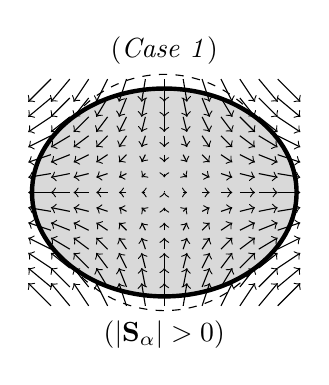
\begin{tikzpicture}[ultra thick,scale=0.6]
        \def\nRows{6}
        \def\nCols{6}
        \draw[dashed,thin] (0,0)circle(2.5);
        \draw[fill=gray!30] (0,0)ellipse(2.8 and 2.2);
        \foreach \x in {-\nRows,...,\nRows} {
            \foreach \y in {-\nCols,...,\nCols} {
                \pgfmathsetmacro\distance{veclen(\x*0.4, \y*0.4)};
                \pgfmathparse{\distance < 2.45 ? "blue" : "white"}
                \edef\colour{\pgfmathresult};
                \ifthenelse{\equal{\colour}{blue}}{                    
                    \draw[thin,->](\x*0.4,\y*0.4)--++(0.08*\x,-0.08*\y);
                }
            }
        }
        \node (txt) at (0,3){(\textit{Case 1})};
        \node (txt) at (0,-3){($|\textbf{S}_\alpha| > 0$)};
    \end{tikzpicture}
     \hfill
    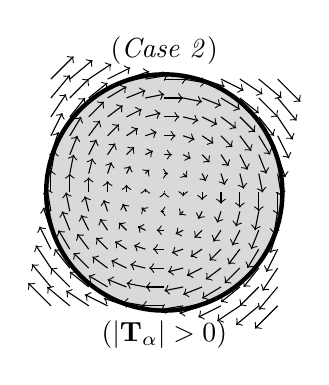
\begin{tikzpicture}[ultra thick,scale=0.6]
        \def\nRows{6}
        \def\nCols{6}
        \draw[fill=gray!30] (0,0)circle(2.5);
        \foreach \x in {-\nRows,...,\nRows} {
            \foreach \y in {-\nCols,...,\nCols} {
                \pgfmathsetmacro\distance{veclen(\x*0.4, \y*0.4)};
                \pgfmathparse{\distance < 2.5 ? "blue" : "white"}
                \edef\colour{\pgfmathresult};
                \ifthenelse{\equal{\colour}{blue}}{                    
                    \draw[thin,->](\x*0.4,\y*0.4)--++(0.08*\y,-0.08*\x);
                }
            }
        }
        \node (txt) at (0,3){(\textit{Case 2})};
        \node (txt) at (0,-3){($|\textbf{T}_\alpha| > 0$)};
    \end{tikzpicture}
    \hfill
    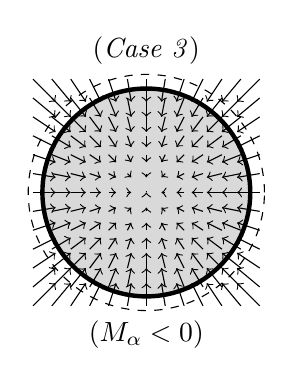
\begin{tikzpicture}[ultra thick,scale=0.6]
        \def\nRows{6}
        \def\nCols{6}
        \draw[dashed,thin] (0,0)circle(2.5);
        \draw[fill=gray!30] (0,0)circle(2.2);
        \foreach \x in {-\nRows,...,\nRows} {
            \foreach \y in {-\nCols,...,\nCols} {
                \pgfmathsetmacro\distance{veclen(\x*0.4, \y*0.4)};
                \pgfmathparse{\distance < 2.3 ? "blue" : "white"}
                \edef\colour{\pgfmathresult};
                \ifthenelse{\equal{\colour}{blue}}{                    
                    \draw[thin,->](\x*0.4,\y*0.4)--++(-0.08*\x,-0.08*\y);
                }
            }
        }
        \node (txt) at (0,3){(\textit{Case 3})};
        \node (txt) at (0,-3){($M_\alpha < 0$)};
    \end{tikzpicture}
    \hfill
    \caption{Graphical representation of the inner kinematics   of an arbitrary particle under three scenarios. 
        The arrows represent the velocity field inside the particle, $\textbf{w}_d^0$, with the corresponding value of the moment of momentum tensor indicated below. 
        The operator $|\ldots|$ refers to the norm of the tensors. 
        According to the inner velocity field:
        (\textit{Case 1}) The particle experiences a mean rate of deformation, resulting in non-zero stretching of momentum along the principal axis of deformation;
        (\textit{Case 2}) The particle is rotating, leading to a non-zero angular momentum vector in the direction of rotation;
        (\textit{Case 3}) The particle undergoes compression, resulting in a negative trace of the moment of momentum.
    }
    \label{eq:scheme}
\end{figure}

% \section{Conservation laws}



% \subsection{Inside the volume}

 


% Let us consider the specific case of the momentum balance, i.e. $q_\alpha = \textbf{p}_\alpha$.
% In this situation, \ref{eq:dt_q_alpha} reads
% \begin{equation}
%     \ddt  \textbf{p}_\alpha
%     = \intO{ \rho_d\textbf{g} }
%     + \intS{ 
%         \left[
%         f_d^0 (\textbf{u}_\Gamma^0-\textbf{u}_d^0)
%          + \bm{\sigma}_d^0%\cdot\textbf{n}_d  
%         %+ \mathbf{\Phi}_d^0 
%         \right] 
%         \cdot \textbf{n}_d },
% \end{equation}
% first term reads as $\intO{ \rho_d\textbf{g} }$ 
% The first term on the right-hand side represents the total weight acting on the particle $\alpha$, 
% the second term represents the total source of momentum due to phase transfer, and it is expressed as, $\intS{ \rho_d \textbf{u}_d^0 (\textbf{u}_\Gamma^0-\textbf{u}_d^0)\cdot\textbf{n}_d }$,
% and the last term $\intS{ \bm{\sigma}_d^0\cdot\textbf{n}_d }$, represents the resultant of the hydrodynamic forces acting on the surface of the particle.
% It is important to note that under this form, the exchange terms are expressed as integrals of dispersed phase fields denoted by the subscript $_d$.
% Nevertheless, depending on the nature of the dispersed phase, these fields may not always be defined.
% For rigid particles the stress within the particle $\bm{\sigma}_d^0$ is indeterminate \citep{guazzelli2011}.  
% Hence, our objective is to express these exchange terms, in terms of the continuous phase field quantities instead of the dispersed phase fields, i.e. in terms of $\mathbf{\Phi}_f^0$ and $\textbf{u}_f^0$ rather than $\mathbf{\Phi}_d^0$ and $\textbf{u}_d^0$. 

%\subsection{On the interfaces}
 

%For completeness, we exposed in \ref{ap:particles_eq} a clear derivation of the mass, momentum and total energy equations for a single particle.
%The derivation takes place using the same hypothesis as it is exposed in \ref{ap:hypothesis}.
%Especially, it is shown that the integration of the kinetic energy jump condition corresponds to the Lagrangian derivative of the particle surface, see \ref{eq:int_u_I2}.

% 

\subsubsection{Zeroth-order conservation laws}

Using the local conservation, \ref{eq:dt_rho}, \ref{eq:dt_rhou_k} and \ref{eq:dt_rhoE_k} into the generic formulation \ref{eq:dt_q_alpha} yields directly the mass momentum and total energy conservation equation for a single particle, namely
\begin{align}
    \ddt m_\alpha
    &= 
    0,\\
    \ddt (m_\alpha \textbf{u}_\alpha)
    &= 
    m_\alpha\textbf{g}
    +  \intS{\bm{\sigma}_d^0 \cdot \textbf{n}_d},\\
    \ddt (m_\alpha E_\alpha)
    &= 
    m_\alpha \textbf{u}_\alpha \cdot \textbf{g}
    +\intS{\textbf{u}_d^0 \cdot \bm{\sigma}_d^0 \cdot  \textbf{n}_d} 
    - \intS{\textbf{q}_d^0 \cdot \textbf{n}_d}. 
\end{align}
As mentioned in \ref{sec:Lagrangian} we now need to derive the particle's surface equations to re-formulate the exchange terms on the right-hand side of these equations. 
It is done by integrating \ref{eq:surface_tension}, \ref{eq:dt_rhoI_uI3} and  \ref{eq:dt_rhoIe_I}  over the surface of the particle, which gives,  
\begin{align}
    \label{eq:int_u_I}
    \intS{\Jump{\bm{\sigma}_k^0} }
    &=
    \intS{\divI\bm\sigma^0_{\Gamma||}} = 0\\
    \label{eq:int_u_I2}
    \intS{\Jump{\textbf{u}_k^0 \cdot \bm{\sigma}_k^0}},
    % = \intS{\Jump{\textbf{w}_k^0 \cdot \bm{\sigma}_k^0}},
    &=
    -\intS{\gamma(\textbf{n}\cdot \textbf{u}_{\Gamma}^0)(\div \textbf{n})}
    = \gamma \ddt s_\alpha,\\
    \label{eq:int_q_I}
    \intS{\Jump{\textbf{q}_k^0}}
    &=
    0,
\end{align}
for the momentum, kinetic, and internal energy of the surface, respectively. 
The second equality of \ref{eq:int_u_I} is demonstrated using \ref{eq:gauss_surface}. 
The second equality of \ref{eq:int_u_I2} is derived noticing that $\intS{\gamma(\textbf{n}\cdot \textbf{u}_{\Gamma}^0)(\div \textbf{n})} = \intS{\divI (\gamma \textbf{u}_I^0)} $ using \ref{eq:gauss_surface} and then the last identity is obtained by using \ref{eq:reynolds_transport}. 
As witnessed by \ref{eq:int_u_I}, on a closed surface the surface tension plays no role in the momentum jump condition.
Additionally, according to \ref{eq:int_u_I2} the work of the surface tension force is equal to $\gamma$ times the rate of change of the area of a given particle. 

Using \ref{eq:int_u_I}, \ref{eq:int_u_I2} and \ref{eq:int_q_I} to reformulate the preceding equations, we easily derive the total mass, momentum, and energy equations for a single particle, 
\begin{align}
    \label{eq:dt_m_alpha}
    \ddt m_\alpha
    &= 
    0\\
    \label{eq:dt_p_alpha}
    \ddt (m_\alpha \textbf{u}_\alpha)
    &= 
    m_\alpha\textbf{g}
    +  \intS{\bm{\sigma}_f^0 \cdot \textbf{n}_d}\\
    \label{eq:dt_E_alpha_tot}
    \ddt (m_\alpha E_\alpha^\text{tot})
    &= 
    m_\alpha \textbf{u}_\alpha \cdot \textbf{g}
    +\textbf{u}_\alpha \cdot \intS{\bm{\sigma}_f^0 \cdot \textbf{n}_d}
    +\intS{\textbf{w}_f^0 \cdot \bm{\sigma}_f^0 \cdot  \textbf{n}_d} 
    - \intS{\textbf{q}_f^0 \cdot \textbf{n}_d}
\end{align}
where  $\intS{  \bm{\sigma}_f^0 \cdot \textbf{n}_d }$ is the resultant of the hydrodynamic forces of the continuous phase, $\intS{\textbf{w}_f^0 \cdot \bm{\sigma}_f^0 \cdot  \textbf{n}_d} $ is the resultant of the work of the continuous phase stresses with the surface velocity, and $\intS{ \textbf{q}_f^0 \cdot \textbf{n}_d }$ is the resultant of the surface heat flux. 
Note that the second term on the right-hand side of \ref{eq:dt_E_alpha_tot} is the work produced by the mean force and the translational motion of the droplets, while $\intS{\textbf{w}_f^0 \cdot \bm{\sigma}_f^0 \cdot  \textbf{n}_d}$ is the work produced by the local forces and local motion of the fluid at the surface of the particle.
Note that these equations do not explicitly account for inter-particle interactions. 
Nevertheless, the surface external stress flux $\bm{\sigma}_f^0$ contains inter-particle forces mediated through the carrier fluid such as lubrication forces and long-range inter-particle forces.

In the spirit of the energy decomposition exposed in the previous section (\ref{eq:dt_rhou_k2} and \ref{eq:dt_rhoe_k}) the total energy equation \ref{eq:dt_E_alpha_tot} can be split into three secondary equations. 
One for the center of mass kinetic energy $u_\alpha^2/2$, another for the particle internal kinetic energy $W_\alpha$, and a last one for the particle internal energy $e_\alpha$, which read
\begin{align}
    \label{eq:dt_u2_alpha}
    \frac{1}{2}\ddt (m_\alpha u_\alpha^2)
    &= 
    m_\alpha\textbf{u}_\alpha\cdot
    \textbf{g}
    + 
    \textbf{u}_\alpha\cdot
    \intS{\bm\sigma_f^0 \cdot \textbf{n}_d},\\
    \label{eq:dt_w2_alpha}
    \ddt (W_\alpha + \gamma s_\alpha)
    &= 
    - \intO{ \bm{\sigma}_d^0 : \grad\textbf{u}_d^0 }
    + \intS {\textbf{w}_f^0 \cdot \bm{\sigma}_f^0 \cdot \textbf{n}_d }
    \\
     \label{eq:dt_e_alpha}
    \ddt (m_\alpha e_\alpha )
    &= 
     \intO{ \bm{\sigma}_d^0 : \grad\textbf{u}_d^0  }
    -  \intS{\textbf{q}_f^0\cdot \textbf{n}_d } 
\end{align}
respectively. 
The first equation is obtained by taking the dot product of \ref{eq:dt_p_alpha} with $\textbf{u}_\alpha$. 
The third equation is directly obtained using the local conservation of $e_k^0$ (\ref{eq:dt_rhoe_k}) and setting $f_d^0 = e_d^0$ in \ref{eq:dt_q_alpha_tot}.
The last equation is obtained by subtracting the first and third equations from \ref{eq:dt_E_alpha_tot}. 
Note that under this form the surface energy is part of the total energy to be conserved, while it could also be treated as a source term using the first formulation of \ref{eq:int_u_I2}.
From this set of equation we can easily see that the rate of dissipation term $\intO{\bm{\sigma}_d^0 : \grad\textbf{u}_d^0}$ represents an energy sink in the equation of $W_\alpha$ while it is a source term in the internal energy equation. 
As it has been observed in the previous section, this term convert the energy of internal motion into molecular agitation. 
However, the interplay between the center of mass kinetic energy and the internal fluctuations is not obvious, indeed \ref{eq:dt_u2_alpha} shares no common term with the heat and internal kinetic energy equation.
We will see that the transfer between these scales is achieved through the fluid-phase pseudo-turbulent energy. 



\subsubsection{Higher-order conservation laws}


Injecting, $f_d^0 = \rho_d$ in the second-order moment equation (derived in \ref{ap:Moments_equations}) we obtain:
\begin{equation}
    \ddt {\textbf{M}_\alpha}=2\textbf{S}_\alpha, 
    \label{eq:dt_M_alpha}
\end{equation}
which is the second-order moment of mass conservation equation. 
From \ref{eq:dt_M_alpha} we deduce that the evolution of the distribution of mass of a particle is solely determined by the stretching of momentum $\textbf{S}_\alpha$. 
This implies that the angular momentum plays no role in the evolution of the second moment of mass. 
This is due to the symmetry of the tensor $\textbf{M}_\alpha$, which must be preserved after differentiation with respect to time.
Nevertheless, that does not mean that the particle angular velocity (noted $\bm\omega_\alpha$ here) has no role in the equation. 
As an example let us consider solid body motion, such that $\textbf{w}_d^0 = \bm\omega_\alpha \times \textbf{r}$, in that case we found, $2\textbf{S}_\alpha = \bm\omega_\alpha \times \textbf{M}_\alpha+ \textbf{M}_\alpha\times \bm\omega_\alpha $. 
Therefore, the angular velocity plays a significant role in the evolution of the second moment of mass equation. 
Additionally, if $\textbf{M}_\alpha$ is constant under change of reference frame, such as for spherical particles where we can write $\textbf{M}_\alpha= \frac{a^2 m_\alpha}{5} \bm\delta$, then $\textbf{S}_\alpha=0$ since $\ddt \textbf{M}_\alpha = 0$ in this situation.
This argument is not restricted to solid particles, thus it is also true for fluid particles with possible inner motion. 
Additionally, applying the trace operator on both sides of \ref{eq:dt_M_alpha}, yields the relation $\ddt {M_\alpha}=\frac{2}{3}\bm\delta : \textbf{S}_\alpha$.
We can state that $M_\alpha = \lambda^\alpha_1(t)+\lambda^\alpha_2(t)+\lambda^\alpha_3(t)$, with $\lambda_i^\alpha$ for $i=1,2,3$, the eigenvalues of $\textbf{M}_\alpha$, as it is a symmetric tensor and thus always diagonalizable.
For undeformable particles, it is evident that the eigenvalues are not functions of time, implying $\ddt M_\alpha = 0$.  
Consequently, $\bm\delta : \textbf{S}_\alpha$ possesses the notable property of being zero whenever the particle shape remains constant, regardless of the orientation.

Now that we have described the kinematics   of the particle shape, let us proceed to derive an equation for the dynamics of the particle shape, i.e. an equation for the moment of momentum. 
This equation is derived injecting $\textbf{Q}_\alpha = \textbf{P}_\alpha$ in \ref{eq:dt_Q_alpha_tot}, it reads, 
\begin{equation}
    \ddt {\textbf{P}_\alpha}
    - \intO{ \rho_d  \textbf{w}_d^0 \textbf{w}_d^0 }
    = 
    - \intO{\bm{\sigma}_d^0}
    - \intS{ 
        \gamma (\bm\delta - \textbf{nn})
    }
    + \intS{ \textbf{r}\bm{\sigma}_f^0\cdot \textbf{n}_d}.
    \label{eq:dt_P_alpha}
\end{equation}
On the left-hands side of \ref{eq:dt_P_alpha} we identify two inertial terms, i.e. the derivative of $\textbf{P}_\alpha$ and the internal velocity term $\intO{\rho_d\textbf{w}_d^0\textbf{w}_d^0 }$.
The inertia of the particle is then balanced by the terms on the right-hand side of the equation, namely: 
the integral of the particle internal stress $\intO{ \bm{\sigma}_d^0}$; 
the integral of the surface tension stress $\intS{ \gamma (\bm\delta- \textbf{nn}) }$; 
and the first moment of the hydrodynamic stress tensor, $\intS{\textbf{r}\bm\sigma_f^0\cdot \textbf{n}}$.
A discussion regarding the physical implications of this equation is provided below. 

The conservation equation of the angular momentum $\bm{\mu}_\alpha$ is obtained by taking the double contracted product of \ref{eq:dt_P_alpha} with $\bm\epsilon$, which directly gives
\begin{equation}
    \ddt\bm{\mu}_\alpha
    =  
    % \textbf{t}_\alpha.
    \intS{ \textbf{r} \times \bm{\sigma}_f^0\cdot \textbf{n}_d }
    \label{eq:dt_mu_alpha}
\end{equation}
Note that every term on the right-hand side of \ref{eq:dt_P_alpha} vanished due to their symmetric nature apart from the skew-symmetric part of the hydrodynamic stress, which is the hydrodynamic torque applied on the particle $\alpha$.
In particular, the surface tension terms do not appear in the angular momentum balance since $\bm\sigma_\Gamma^0 = \gamma (\bm\delta-\textbf{nn})$ is symmetric, which is consistent with the findings of \citet{hesla1993note}. 
As a consequence, the surface tension does not affect the angular momentum regardless of the particle's shape. 
In the literature, it is common to include the torque due to inter-particular interactions in the angular momentum balance, as is done in \citet{jackson1997locally} and \citet{zhang1997momentum}.
In our case note that $\bm{\sigma}_f^0$ contains short-range hydrodynamic interaction forces. 

Taking the double contracted product of \ref{eq:dt_P_alpha} with the tensor $\bm\delta$ and using \ref{eq:dt_M_alpha}, yields directly  
% \begin{equation}
%     \frac{1}{2}\ddt^2 {M_\alpha}
%     - \frac{1}{3}\intO{ \rho_d \textbf{w}_d^0 \cdot \textbf{w}_d^0}
%     = 
%     \intO{p_d^0} 
%     % - \frac{1}{3}\intS{p_f^0 \textbf{r}\cdot \textbf{n}}
%     - \frac{2}{3} \gamma s_\alpha
%     - \frac{1}{3}\intS{p_f^0 \textbf{r}\cdot \textbf{n}}
%     + \frac{1}{3}\intS{\textbf{r}\cdot\bm\tau_f^0\cdot \textbf{n}},
%     \label{eq:dt_D_alpha}
% \end{equation}
\begin{equation}
    \frac{3}{2}\frac{d^2 M_\alpha}{dt^2}
    - \intO{ \rho_d \textbf{w}_d^0 \cdot \textbf{w}_d^0}
    = 
    - \intO{\bm\sigma_d^0:\bm\delta} 
    % - \frac{1}{3}\intS{p_f^0 \textbf{r}\cdot \textbf{n}}
    - \gamma 2 \intS{}
    % - \frac{1}{3}\intS{p_f^0 \textbf{r}\cdot \textbf{n}}
    + \intS{\textbf{r}\cdot\bm\sigma_f^0\cdot \textbf{n}}.
    \label{eq:dt_D_alpha}
\end{equation}
\ref{eq:dt_D_alpha}, corresponds to the isotropic work balance over the volume and surface of the particle. 
According to \ref{eq:dt_D_alpha}, the rate of compression of a particle, denoted by the second derivative of $M_\alpha$ evolves according to : 
the internal inertial term, $\intO{\rho_d \textbf{w}_d^0 \cdot \textbf{w}_d^0 }$;
the particle internal pressure $\intO{\bm\sigma_d^0:\bm\delta}$; 
the surface energy $\gamma\intS{  }$; 
and the trace of the hydrodynamic first moment $\intS{\textbf{r}\cdot\bm\sigma_f^0\cdot \textbf{n}}$.
If one considers spherical particles composed of compressible fluid, \ref{eq:dt_D_alpha} transforms into the Rayleigh-Lamb-Plesset equation as demonstrated in the unpublished work of \citep{danielcours}. 
In the steady-state regime, this reduces to the Young-Laplace equation, as indicated by the presence of the first three terms on the right-hand side of \ref{eq:dt_D_alpha}. 

% \tb{
%     As an example we now consider the \textit{Rayleigh-Lamb-Plesset} equation for spherical bubbles with radius $a_\alpha(t)$. 
%     As the droplets remain spherical while keeping a constant mass the moment of momentum and inner velocity field can be expressed, 
%     \begin{align*}
%         M_\alpha
%         = \frac{m_\alpha}{5} a^2_\alpha(t),
%         && 
%         \textbf{w}_d^0
%         = \frac{d a_\alpha}{dt}\frac{\textbf{r}}{a_\alpha(t)},
%         \label{eq:expr1}
%     \end{align*}
%     where it is empathized that the radius $a_\alpha(t)$ is time-dependent. 
%     The stress inside the bubbles might be expressed as compressible Newtonian fluids with no resistance to shear such that 
%     \begin{equation}
%         \bm\sigma_d^0 
%         = 
%         - p_d^0 \bm\delta
%         - \lambda_d (\div \textbf{u}_d^0) \bm\delta
%         % + \mu_d \left[\grad \textbf{u}_d^0 + (\grad \textbf{u}_d^0)^\dagger\right]
%         = 
%         - p_d^0 \bm\delta
%         - \frac{3 \lambda_d}{a_\alpha} \frac{d a_\alpha}{dt}  \bm\delta
%         % + \mu_d \left[\grad \textbf{u}_d^0 + (\grad \textbf{u}_d^0)^\dagger\right]
%         \label{eq:StressBubbles}
%     \end{equation}
%     where $\lambda_d^0$ is the volume viscosity of the dispersed phase. 
%     Assuming incompressible Newtonian fluid for the continuous phase and injecting the expressions \ref{eq:StressBubbles} and \ref{eq:expr1} into \ref{eq:dt_D_alpha} yields, 
%     \begin{equation}
%         \frac{1}{5} \rho_d^0 a_\alpha \frac{d^2 a_\alpha}{dt^2} 
%         - 
%         \frac{1}{a_\alpha} \frac{d a_\alpha}{dt} 
%         \left(
%             3 \lambda_d
%             + 2 \mu_f 
%         \right)
%         = 
%         +  \frac{1}{v_\alpha}\intO{p_d^0}
%         -  \frac{1}{s_\alpha}\intS{p_f^0}
%         - \gamma  \frac{2}{a}
%     \end{equation}
%     By expressing the fluid pressure on the surface in terms of the far field pressure (see daniel) one obtain the \textit{Rayleigh-Lamb-Plesset} equation. 
%     In the static regime we recover laplace eq
% }

Taking the symmetric part of \ref{eq:dt_P_alpha}, and making use of \ref{eq:dt_M_alpha}, yields a dynamical balance equation for $\textbf{M}_\alpha$, namely
% \begin{multline}    
%     \frac{1}{2}\ddt^2{\textbf{M}_\alpha^\text{dev}}
%     - \intO{\left(
%         \rho_d\textbf{w}_d^0 \textbf{w}_d^0
%         - \rho_d\frac{1}{3}(\textbf{w}_d^0 \cdot \textbf{w}_d^0)\bm\delta\right)}
%     =  
%         - \mu_d \intO{\textbf{e}_d^0}
%         - \intS{\gamma\left(\frac{1}{3}\bm\delta-\textbf{nn}\right)}\\
%         + \frac{1}{2}\intS{\left(\textbf{r}\bm\sigma_f^0+ \bm\sigma_f^0\textbf{r} - \frac{2}{3}(\bm\sigma_f^0\cdot \textbf{r})\bm\delta\right)\cdot \textbf{n}}
%     \label{eq:dt_S_alpha}
% \end{multline}
\begin{equation}    
    \frac{1}{2}\frac{d^2 \textbf{M}_\alpha}{dt^2}
    - \intO{ \rho_d  \textbf{w}_d^0 \textbf{w}_d^0 }
    = 
    - \intO{\bm{\sigma}_d^0}
    - \intS{\gamma (\bm\delta - \textbf{nn})}
    + \frac{1}{2}\intS{(\textbf{r}\bm{\sigma}_f^0+\bm{\sigma}_f^0 \textbf{r})\cdot \textbf{n}_d}.
    \label{eq:dt_S_alpha}
\end{equation}
On the left-hand side of \ref{eq:dt_S_alpha}, we recover the symmetric part of the inertial contributions. 
In opposition to \ref{eq:dt_P_alpha} we could substitute the term $\ddt (\textbf{P}_\alpha+\textbf{P}_\alpha^\dagger)$ initially present in the equation by $\ddt^2 \textbf{M}_\alpha$ using \ref{eq:dt_M_alpha}. 
Consequently, \ref{eq:dt_S_alpha} is a second-order partial differential equation for the droplet mean deformation. 
In our case, only the external contribution $\intS{\textbf{r}\bm\sigma_f^0\cdot \textbf{n}}$ is responsible for the generation of angular momentum, see \ref{eq:dt_mu_alpha}.
Taking the symmetric part of this tensor ultimately removes this contribution. 
Thus, on the right-hand side of \ref{eq:dt_S_alpha}, we identify the terms responsible for the droplet deformation exclusively.
Therefore, \ref{eq:dt_S_alpha} must be interpreted as an equation for the shape of the particle, represented by the tensor $\textbf{M}_\alpha$.
One might immediately recognize that \ref{eq:dt_S_alpha} is in fact an extension of \citet{batchelor1970stress}'s famous result, 
\begin{equation}
    \intO{\bm{\sigma}_d^0}
    + \intS{\gamma(\bm\delta - \textbf{nn})}
    = \frac{1}{2}\intS{(\textbf{r}\bm\sigma_f^0+\bm\sigma_f^0\textbf{r})\cdot \textbf{n}},
    \label{eq:Batchelor}
\end{equation}
but with the consideration of the inertia of the particle.
\ref{eq:Batchelor} is particularly useful to compute the unknown internal stress within solid particles (for which $\gamma = 0$), in terms of surface integral, i.e. the stresslet $\intS{(\textbf{r}\bm\sigma_d^0+ \bm\sigma_d^0\textbf{r})\cdot \textbf{n}}$.
This relation is the main tool used to express the bulk stress of a suspension.
It eventually leads to the computation of the famous Einstein equivalent viscosity, upon having a closed expression for the average of $\intS{(\textbf{r}\bm\sigma_d^0+ \bm\sigma_d^0\textbf{r})\cdot \textbf{n}}$ \citep{guazzelli2011}. 
In the inertial case, due to the limited degree of freedom of solid particles, the tensors $\textbf{M}_\alpha$ and the inner velocity field $\textbf{w}_d^0$ are fully determined by \ref{eq:dt_M_alpha} and \ref{eq:dt_mu_alpha}, indicating that $\textbf{M}_\alpha$ and $\textbf{w}_d^0$ can be used in \ref{eq:dt_S_alpha} not as unknowns but as source terms. 
Consequently, for solid particles, \ref{eq:dt_S_alpha} must be interpreted as a generalized equation for the undefined stress $\bm\sigma_d^0$ integrated on the volume of the particles.
Whether it is solid or fluid particles \ref{eq:dt_S_alpha} becomes particularly relevant for expressing the averaged stress within an inertial suspension in terms of Lagrangian properties, as discussed in the next chapter. 

It is now clear that if the surface tension forces play no role in the linear and angular momentum equation, however, it impacts the moment of momentum $\textbf{P}_\alpha$ or more specifically its symmetric part $\textbf{S}_\alpha$.
Thus, the surface tension force impacts the hydrodynamic behavior of a particle solely through its action on $\textbf{S}_\alpha$, which is related to the shape of a particle represented by $\textbf{M}_\alpha$, through \ref{eq:dt_M_alpha}.
In \ref{ap:Moments_equations} we show how to derive the higher-order moment of momentum equations, which can also be viewed as formulas for the higher moments of the internal particle stress distribution. 
It is interesting to mention that in a recent study of \citet{dolata2021faxen} and \citet{zhou2020lamb} they make use of the first two moments of momentum equations hidden into another but equivalent form, valid in the Stokes flow regime. 



% \section{The two-fluid model}
\label{ap:two-fluid_model}

% \subsubsection{Volume equation}
Using the generic formulation \ref{eq:avg_dt_chi_f} and the local expression of the mass, momentum and total energy equation, i.e. : \ref{eq:dt_rho},\ref{eq:dt_rhou_k} and \ref{eq:dt_rhoE_k} we easily find the averaged form of the mass, momentum and total energy equation.
They read, 
\begin{align}
    \label{eq:dt_avg_rho}
    \pddt (\phi_k \rho_k)  
    + \div (
        \phi_k \rho_k\textbf{u}_k
    )
    &= 
    0\\
    \label{eq:dt_avg_rhou_k}
    \pddt (\phi_k \rho_k\textbf{u}_k)  
    + \div (
        \phi_k \rho_k\textbf{u}_k\textbf{u}_k
        + \bm{\sigma}_k^\text{eq}
    )
    &= 
    \phi_k \rho_k \textbf{g} 
    +  \avg{\delta_I \bm{\sigma}_k^0 \cdot \textbf{n}_k}\\
    \label{eq:dt_avg_rhoE_k}
    \pddt (\phi_k\rho_kE_k)  
    + \div (
        \phi_k\rho_kE_k\textbf{u}_k
        + \bm{q}_k^\text{eq}
        + \textbf{u}_k \cdot \bm{\sigma}_k^\text{eq}
        % - \textbf{u}_k^0 \cdot \bm{\sigma}_k^0 
        % + \textbf{q}_k^0
        )
    &= 
    \phi_k \rho_k\textbf{u}_k \cdot \textbf{g} 
    + \avg{\delta_I (\textbf{u}_k^0 \cdot \bm{\sigma}_k^0 - \textbf{q}_k^0)\cdot \textbf{n}_k}
\end{align} 
with the equivalent stress and heat flux defined as, 
\begin{align*}
    &\bm{\sigma}_k^\text{eq}
    = 
     \rho_k\avg{\chi_k \textbf{u}_k'\textbf{u}_k'}
      - \phi_k \bm{\sigma}_k,%- n_p \textbf{M}_p
    &\textbf{q}_k^\text{eq}
    =\textbf{q}_k^\text{e} +\textbf{q}_k^\text{k},  \\
    &\textbf{q}_k^\text{e}
    = \rho_k \avg{\chi_k\textbf{u}_k' e_k'} 
    + \phi_k\textbf{q}_k,
    &\textbf{q}_k^\text{k}
    = \rho_k \avg{\chi_k \textbf{u}_k' k_k} 
    - \avg{\chi_k \textbf{u}_k' \cdot \bm{\sigma}_k^0}.
\end{align*}
% The main differences between these equations and their microscale counterpart, is that : (1) we have introduced a pre factor $\phi_k$ in front of most of the terms
% (2) an additional stress is present, that is the covariance between the quantity to be conserved and the velocity. 
% (3) A new source term appear on the RHS accounting for the exchange across the phases. 

The terms $\avg{\chi_k \textbf{u}_k'\textbf{u}_k'}$ will be referred as the Reynolds stress or pseudo turbulent stress. 
It has a fundamental importance in the multiphase flow problem and as we see now its trace is related to the mean kinetic energy. 
Indeed, the phase averaged total energy can be further decompose into three energy components, that is,  
\begin{align}
    E_k = e_k + k_k + u_k^2/2
    \label{eq:E_def}
\end{align}
where $k_k$ is the pseudo-turbulent kinetic energy defined as, $\phi_k k_k = \frac{1}{2}\avg{\chi_k \textbf{u}_k'\cdot \textbf{u}_k'}$. 
Each of the components of the total energy represent the averaged agitation at different scales. 
From molecular agitation which quantified by $e_k$, to the macroscopic scale agitation or kinematic energy $u_k^2$, and in between we find the pseudo turbulent energy $k_k$ which represents the local scale velocity fluctuation. 
To fully describe the averaged total energy one must add at least a supplementary equation either for $k_k$ or $e_k$ assuming \ref{eq:dt_avg_rhoE_k} is solved. 
Using \ref{eq:dt_avg_rhou_k} dotted with $\textbf{u}_k$ yields an equation for the mean kinetic energy. 
Averaging \ref{eq:dt_rhoe_k} yields un equation for $e_k$.  
Then, subtracting these two equations to \ref{eq:dt_avg_rhoE_k} gives us an equation for $k_p$. 
The kinetic energy, pseudo turbulent and internal averaged equations read as, 
\begin{align}
    \label{eq:dt_avg_uk2}
    &\pddt (\phi_k \rho_ku_k^2/2)  
    + \div (
        \phi_k \rho_k\textbf{u}_ku_k^2/2
        + \textbf{u}_k \cdot \bm{\sigma}_k^\text{eq}
    )
    = 
    \bm{\sigma}_k^\text{eq} : \grad \textbf{u}_k
    + \phi_k \rho_k \textbf{u}_k\cdot \textbf{g} 
    +  \textbf{u}_k\cdot \avg{\delta_I \bm{\sigma}_k^0 \cdot \textbf{n}_k},\\
    \label{eq:dt_avg_kk}
    &\pddt (\phi_k\rho_kk_k)  
    + \div (
        \phi_k\rho_kk_k\textbf{u}_k
        + \textbf{q}_k^\text{k} 
        )
    = 
    - \avg{\chi_k\bm{\sigma}_k^0 : \grad \textbf{u}_k^0}
    - \bm{\sigma}_k^\text{eq} : \grad \textbf{u}_k
    + \avg{\delta_I \textbf{u}_k' \cdot \bm{\sigma}_k^0 \cdot \textbf{n}_k},\\
    \label{eq:dt_avg_ek}
    &\pddt (\phi_k\rho_ke_k)  
    + \div (
        \phi_k \rho_ke_k\textbf{u}_k
        +
        \textbf{q}_k^\text{e} 
        )
    = 
    \avg{\chi_k\bm{\sigma}_k^0 : \grad \textbf{u}_k^0}
    - \avg{\delta_I \textbf{q}_k^0 \cdot \textbf{n}_k},
\end{align}
respectively. 
This derivation is in agreement with \citet{morel2015mathematical}. 
Under this form the energy transfer across scale is clear. 
Indeed, the term $\bm{\sigma}_k^\text{eq} : \grad \textbf{u}_k$ act as a sink term in \ref{eq:dt_avg_uk2} and a source term in \ref{eq:dt_avg_kk}, while the averaged diffusive terms $\avg{\chi_k\bm{\sigma}_k^0 : \grad \textbf{u}_k^0}$ is a sink in \ref{eq:dt_avg_kk} and a source in \ref{eq:dt_avg_ek}. 
To determine the total energy only two of the four energy equations must be solved. 
In practice, it is useful to solve one equation for $k_k$ since it is useful for the Reynolds stress modeling since $\avg{\chi_k \textbf{u}_k^0 \textbf{u}_k^0}: \bm\delta = 2 k_k$, and another for $e_k$ since $u_k^2$ is already determined by the momentum equation. 

% \subsubsection{Averaged surface equations}
The volume averaged equations must be completed by an averaged surface transport equation.  
For this purpose we multiply \ref{eq:surface_tension}, \ref{eq:dt_rhoIe_I} and \ref{eq:dt_rhoI_uI3} by $\delta_I$ and apply the average operator.
By considering the topological equations we obtain the  momentum, kinetic and internal energy averaged surface equations, namely
\begin{align}
    \label{eq:dt_avg_uI}
    \avg{\delta_I \Jump{\bm{\sigma}^0_k}}
    &= -\gamma \div \avg{\delta_I (\bm\delta - \textbf{nn})},\\
    \label{eq:dt_avg_gamma}
    \avg{\delta_I \Jump{\textbf{u}_k^0 \cdot \bm{\sigma}^0_k}}
    &= - \gamma \left[
        \pddt \avg{\delta_I}
        +  \div \avg{\delta_I (\textbf{u}_{I}^0 \cdot \textbf{n})\textbf{n} },
    \right]\\
    \avg{\delta_I \Jump{\textbf{q}^0_k}}
    &= 0
\end{align}
respectively. 
The first equation represents the contribution of the surface tension stresses to the bulk momentum equation.
The second equation represents the amount of energy stored as surface deformation.
And the last equation witnesses of the continuity of heat flux through the interface. 

% 

\section{The bulk stress in dispersed multiphase flow}
\label{sec:symetric_stress}


One of the major questions in suspension dynamic raised by several authors, is the evaluation of the bulk stress or equivalent stress tensor of a suspension, see \citep{batchelor1970stress, prosperetti2006stress,zhang1997momentum,nadim1996concise} and more recently \citet{dolata2020heterogeneous}. 
Specifically, we seek to express the bulk stress in the suspension in terms of particle-averaged quantities. 
Only then it is possible to derive closures for the stress. 
Therefore, in this subsection we derive an expression for the bulk stress of an emulsion in terms of the Lagrangian particle quantities derived in the two previous sections. 
For the sake of generality in this section we consider that the flow is subjected to an arbitrary body force $\textbf{b}$. 

\subsection{The bulk stress formulation}

Before proceeding further, it is useful to clarify what we mean exactly by the \textit{bulk stress}.
The \textit{bulk stress} tensor is the force per unit of surface applied on the fluid and on the particles phases, having the form $\div \bm{\sigma}^\text{eq}_m$, which added to the total external force, balances exactly the material derivative of the mixture momentum, namely: $\pddt (\rho \textbf{u}_m) + \div (\rho \textbf{u}_m\textbf{u}_m)$. 
This definition of the bulk stress implies that the external body force term $\textbf{b}$ cannot be decomposed into a vector plus a divergence of a tensor, in which case the latter would just contribute to $\bm{\sigma}^\text{eq}$.
Thus, in this definition $\textbf{b}$ must be reformulated since $\textbf{b} = \phi_f \textbf{b}_f+\phi_d \textbf{b}_d$ and that the term $\phi_d \textbf{b}_d$ can be decomposed into a Taylor series according to \ref{eq:f_exp}. 
Therefore, the momentum equation is obtained by setting $\rho \textbf{g} = \textbf{b}$ in \ref{eq:dt_avg_rhou} and by reformulating the body force term accordingly we obtain,
\begin{align}
    \label{eq:momentum_bulk}
    \pddt (\rho^0 (\textbf{u}_m)_i)
    + \partial_j  [\rho (\textbf{u}_m \textbf{u}_m)_{ij}
    + (\bm\sigma_{m}^\text{eq})_{ij}]
    &= \left[\phi_f \textbf{b}_f + \pOavg{\textbf{b}}\right]_i
    % \epsilon_{ijk} \sigma_{jk}
    % &= 0 
    % \label{eq:angular_momentum_bulk}
\end{align}
% Indeed, in the averaged angular momentum equation we have assumed that no-body torque exist at the local scale making the skew-symmetric part of $\sigma_{jk}^0$ equal to $0$ \citet{leal2007advanced}. 
% Taking the average of the bulk momentum and angular momentum equation gives directly, 
Where we have defined the effective stress of the suspension as,
\begin{multline}
    \bm{\sigma}_m^\text{ed}
    = 
    \avg{\rho^0\textbf{u}_m'\textbf{u}'_m}
    + \phi_fp_f\bm\delta
    - 2\mu_f\textbf{e}
    - \phi_d(\bm{\sigma}_d - 2\mu_f \textbf{e}_d)
    - \phi_\Gamma \bm{\sigma}_\Gamma\\
    + \pOavg{\textbf{r}\textbf{b}_d^0}
    -\frac{1}{2} \div \pOavg{\textbf{rr}\textbf{b}_d^0} + \ldots
    \label{eq:sigma_bulk}
\end{multline}
% where we have used the relation 
The first term corresponds to the Reynolds stress, and the second third and fourth terms are obtained by noticing that 
$
    \phi_f \bm\sigma_f
    = -\phi_f p_f \bm\delta
    + 2\mu_f \textbf{e}
    - 2 \mu_f \phi_d \textbf{e}_d 
$
where $\phi_f p_f$ is the mean fluid pressure and $\textbf{e} = \grad \textbf{u} + ^\dagger(\grad \textbf{u})$ the averaged strain rate of the suspension. 
% The last two terms of \ref{eq:sigma_bulk} have been obtained by expanding the body force term $\phi_d \textbf{b}_d$ originally present on the right-hand side of \ref{eq:momentum_bulk} in a Taylor expansion according to \ref{eq:f_exp}. 
Additionally, we considered that the local angular momentum balance follows  $\epsilon_{ijk} \sigma_{jk}^0 = 0$. 
Due to the linearity of the ensemble average operator we deduce that the averaged stress also respects $\epsilon_{ijk} \sigma_{jk}$.
The interface stress also follows this condition since $\bm\sigma_I^0 = \gamma (\bm\delta - \textbf{nn})$ which is by definition symmetric.  
Thus, we can already conclude that the first five terms on the right-hand side of \ref{eq:sigma_bulk} are by definition symmetric since they are just averaged quantities of tensors which are by definition symmetric. 
Consequently, the only possible skew-symmetric contribution to the suspension stress must arise from the last two terms on the right-hand side of \ref{eq:sigma_bulk}.  
The discussion regarding the symmetry of $\bm\sigma^{eq}_m$ will be addressed in more detail at the end of this section. 

% The first moment contribution to the skew symmetric part is given by 
% \begin{equation}
%     \pOavg{\textbf{r}\textbf{b}_d^0 - \textbf{b}_d^0 \textbf{r}}. 
%     \label{eq:body_torque}
% \end{equation}
% This term corresponds to the averaged torque generated by the body force field $\textbf{b}^0$ on the particles. 
% Thus, all body force fields generating body torque will induce self toque in the suspension. 

% For the higher moment of body force the reasoning is slightly different.
% We use a methodology similar to \citep{lhuillier1992volume,lhuillier1996contribution} to re express the second and higher moment of the body force.  
% For convenience let us note 
% \begin{equation}
%     B_{ijk}
%     = \pOavg{\textbf{rr}\textbf{b}_d^0} - \frac{1}{3}\div \pOavg{\textbf{rrr}\textbf{b}_d^0} + \ldots
% \end{equation}
% % which represent the second plus the divergence of the higher order moment of the body forces. 
% Since this tensor is the sum of the second plus the higher moment it is not symmetric on any index. 

% We recall that the carrier fluid is a Newtonian fluid, therefore we may express the fluid phase stress as, 
Let us now present the bulk stress formulation in the \textit{hybrid} form, meaning in terms of particle-average quantities.  
The divergence of the dispersed phase stresses present in \ref{eq:momentum_bulk} through \ref{eq:sigma_bulk} may be expressed using \ref{eq:f_exp}, it gives
\begin{align}
    \label{eq:exp_e2}
    \partial_k (\phi_d \textbf{e}_d)_{ik} 
    &=  \partial_k\pSavg{ (\textbf e_d^0)_{ik} }
        -\frac{1}{2} \partial_k\partial_j \pSavg{ r_j (\textbf e_d^0)_{ik} +r_k (\textbf e_d^0)_{ij} }
        + \ldots  \\
    \label{eq:exp_sigma22}
    \partial_k (\phi_d \bm\sigma_d)_{ik}
    &=  \partial_k\pOavg{ (\bm\sigma_d^0)_{ik}}
    -\frac{1}{2} \partial_k\partial_j
    \pOavg{ r_j(\bm\sigma^0_d)_{ik} + r_k(\bm\sigma^0_d)_{ij}}
    + \ldots  \\
    \label{eq:exp_sigmaI2}
    \partial_k (\phi_\Gamma \bm\sigma_I)_{ik} 
    &=  \partial_k\pSavg{ (\bm\sigma_I^0)_{ik} }
        -\frac{1}{2} \partial_k\partial_j \pSavg{ r_j (\bm\sigma_I^0)_{ik} +r_k (\bm\sigma_I^0)_{ij} }
        + \ldots  
\end{align}
Note that we reformulated the second terms on the right-hand side of \ref{eq:exp_e2},\ref{eq:exp_sigma22} and \ref{eq:exp_sigmaI2} by retaining only their symmetric part since these terms must remain symmetric in the index $k$,$j$ due to the double contraction with the operator $\partial_k\partial_j$. 
Now we can use the first moment of momentum conservation \eqref{eq:dt_S_alpha} and the second moment of momentum equation (derived in \ref{ap:Moments_equations}, see \eqref{eq:second_momoent_of_momentum}) to reformulate the particle internal stresses, this yields,  
\begin{multline}
    \intS{ (\bm{\sigma}_\Gamma^0)_{ik}}
    +\intO{ (\bm{\sigma}_d^0)_{ik}}
    = 
    \intO{ \rho_d 
    (\textbf{w}_d^0\textbf{w}_d^0  )_{ik}
    }
    -\frac{1}{2}\left(\frac{d^2 \textbf{M}_\alpha}{dt^2} \right)_{ik}\\
    +\frac{1}{2}\intO{ \left[
        (\textbf{b}_d^0)_i
        r_k 
        + (\textbf{b}_d^0)_k
        r_i
    \right]}
    +
    \frac{1}{2}\intS{ \left[
        (\bm{\sigma}_1^0 \cdot \textbf{n}_d)_i r_k
        + (\bm{\sigma}_1^0 \cdot \textbf{n}_d)_k r_i
    \right]
    }
    \label{eq:dt_P1_alpha_bis}
\end{multline}
\begin{multline}
    \intO{ r_{j}(\bm{\sigma}^0_d)_{ik}+r_{k}(\bm{\sigma}^0_d)_{ji}}
    +\intS{ r_{j}(\bm{\sigma}^0_I)_{ik}+r_{k}(\bm{\sigma}_\Gamma^0)_{ji}}
    = 
    - \ddt\intO{ \rho_d (\textbf{u}_d^0)_i r_j r_k }
    \\
    + \intO{ \left[
        \rho_d (\textbf{u}^0_d\textbf{r}\textbf{w}_d^0)_{ijk} + \rho_d (\textbf{u}^0_d\textbf{r}\textbf{w}_d^0)_{kji}
    \right]}
    +\intS{  r_{k}r_{j} (\bm{\sigma}_1^0\cdot\textbf{n}_d)_i }
    + \intO{ r_{k}r_{j}  \rho_d (\textbf{b}_d^0)_i } 
    \label{eq:dt_P2_alpha_bis}
\end{multline}
By using an arbitrary order of moment of momentum equation (derived in \ref{ap:Moments_equations}) one can substitute any volume integral of the particle stress appearing in the expansion \ref{eq:exp_sigma22} into particles' kinematic properties plus the hydrodynamic moment of the fluid phase. 
Substituting \ref{eq:dt_P2_alpha_bis} and \ref{eq:dt_P1_alpha_bis} into \ref{eq:sigma_bulk} yields, 
\begin{multline}
    (\bm{\sigma}^\text{eq}_m)_{ik}
    = 
    \underbrace{
        % \left[
        \phi_f p_f 
        % + \frac{1}{3}\pOavg{\textbf{r}\cdot\bm{\sigma}_f^0 \cdot \textbf{n}_d} 
    % \right]
    \delta_{ik}
    - \mu_f e_{ik} 
    }_\text{Newtonian contribution}
    + \underbrace{\avg{\rho^0 \textbf{u}'_m\textbf{u}'_m}_{ik}}_\text{Bulk Reynolds stress}
    % + \mu_f \phi_2 e_{2,ik}. 
    + \underbrace{\epsilon_{ikj} \frac{1}{2}\pSavg{ (\textbf{b}_d^0 \times \textbf{r})_j}}_\text{Particles body torque}\\
    - \frac{1}{2}\underbrace{\pSavg{\left[
        (\bm{\sigma}_f^0 \cdot \textbf{n}_d)_kr_i  
        + (\bm{\sigma}_f^0 \cdot \textbf{n}_d)_i r_k
        % - \frac{2}{3}(\textbf{r}\cdot\bm{\sigma}_f^0 \cdot \textbf{n}_d)\delta_{ik}
    \right]}
    + 2 \mu_f \pOavg{(\textbf{e}_d^0)_{ik}}}_\text{Averaged Stresslet}\\
    - \underbrace{\pOavg{ \rho_d (\textbf{w}_d^0\textbf{w}_d^0  )_{ik}}
    + \pavg{\frac{d^2 \textbf{M}_{ik}}{dt^2}  }}_\text{particles inertia}
    + \underbrace{\frac{1}{2} (\div\bm{\Sigma})_{ik}}_\text{Inhomogeneous stresses}
    \label{eq:stress_bulk_explicit}
\end{multline}
with,
\begin{multline}
    \bm{\Sigma}
    = 
    - \pavg{\ddt\intO{ \rho_d (\textbf{u}_d^0)_i r_j r_k }}
    + \pOavg{ 
        \rho_d \left[
        (\textbf{u}^0_d\textbf{r}\textbf{w}_d^0)_{ijk} +  (\textbf{u}^0_d\textbf{r}\textbf{w}_d^0)_{kji}
    \right]
    }\\
    +\pSavg{  (\bm{\sigma}_f^0 \cdot \textbf{n}_d)_i r_{j}  r_{k}  }
    - 2 \mu_f \pOavg{[( \textbf{e}_d^0 \textbf{r})_{ikj}
    + ( \textbf{e}_d^0 \textbf{r})_{ijk}]} + \div[\ldots]
    \label{eq:Sigma_inhomo}
\end{multline}
We can note that the body force terms present in \ref{eq:sigma_bulk} and \ref{eq:dt_P2_alpha_bis} canceled each other in \ref{eq:Sigma_inhomo}. 
Under this form the different contributions to the suspension stress are explicit. 
The first contribution is the averaged continuous phase Newtonian stress. 
The second term is the  contribution from the total phase fluctuation to the suspension stress, including the particle internal fluctuation. 
The third term is the skew-symmetric part of the first moment of the body forces, in this study $\textbf{b}^0 = \rho^0 \textbf{g}$ thus this term vanishes for any kind of particles. 
The symmetric part of the hydrodynamic stresses together with the particle's internal shear rate form what is called: the Stresslet \citep{pozrikidis1992boundary}. 
Especially, we see in the next section that this term is related to the Einstein equivalent viscosity (see \ref{eq:fluid_phase_stress}). 
The first two terms on the third line of \ref{eq:stress_bulk_explicit} are the particle inertia contribution to the suspension stresses. 
This includes the second-order derivative of the particle shape represented by $\textbf{M}_\alpha$ and the internal particle motions. 
As discussed in the previous section this term is solely related to the inertia induced by change of orientation or deformation of the particles. 
Finally, the last term of the expression represents the contribution to the stress from all the higher moments related to the particles, it includes the moments related to the internal velocity or external hydrodynamic forces.  
Notice that since this term appears under the divergence operator it is non-zero only for Inhomogeneous suspension, therefore we call it the \textit{Inhomogeneous stresses}. 
The formulation of the bulk stress given by \ref{eq:stress_bulk_explicit} is formally equivalent to equation (8) and (12) of \citet{lhuillier1996contribution} and equation (8.2) of \citet{zhang1997momentum}.
The equivalence with \citet{zhang1997momentum} is not obvious as they use different decompositions for most of the terms. 
Although the relation \ref{eq:stress_bulk_explicit} is not new, the derivation presented here is original since the physical significance of all terms is explicit because it is derived in terms of particle-averaged quantities.

    
\subsection{Additional simplifications}

The averaged rate of strain, \textbf{e}, present in \ref{eq:stress_bulk_explicit} involves the averaged bulk velocity \textbf{u}. 
However, the momentum equation's purpose is to be solved for the Favre averaged velocity fields $\textbf{u}_m$. 
This means that two velocity fields are present in this equation meaning that a supplementary equation is needed to recover $\textbf{u}$ from $\textbf{u}_m$ and inversely. 
This inconsistency is easily fixed by noticing that, $\rho \textbf{u} = \sum_k \rho_k \phi_k \textbf{u}_k$, which implies that, 
\begin{equation}
    \textbf{u}=\rho \textbf{u}_m\sum_k \frac{1}{\rho_k \phi_k}
\end{equation}
Thus, we can recover the velocity field \textbf{u} needed in the expression of \textbf{e} through $\textbf{u}_m$ and the volume fractions. 

The only term in \ref{eq:stress_bulk_explicit} that is not expressed in terms of particle averaged quantities is the \textit{Reynolds stress} tensor, $\avg{\rho^0 \textbf{u}'_m\textbf{u}'_m}$. 
Indeed, the local field $\textbf{u}_m' = \textbf{u}^0 - \textbf{u}_m$ involves the local velocity fields within the particle.
From an experimental point of view, this quantity is difficult if not impossible to quantify.  
Therefore, it is interesting to reformulate this \textit{bulk Reynolds stress} in terms of continuous fluid phase averaged Reynolds stress and a stress related to particle averaged properties. 
This is easily done by noticing that, 
\begin{equation*}
    \avg{\rho^0 \textbf{u}'_m\textbf{u}'_m}
    = 
    \avg{\chi_f \rho_f \textbf{u}_f'\textbf{u}_f'}
    + \phi_f \rho_f \textbf{u}_f\textbf{u}_f
    - \rho \textbf{u}_m\textbf{u}_m
    + \avg{\chi_d \rho_d \textbf{u}_d^0\textbf{u}_d^0}
    \label{eq:u_mu_m}
\end{equation*}
We can notice that $\avg{\chi_f \rho_f \textbf{u}_f'\textbf{u}_f'}$ is the fluid phase Reynolds stress introduced in \ref{eq:dt_avg_rhou_k}. 
Regarding the last term of \ref{eq:u_mu_m} it can be reformulated as, 
\begin{equation*}
    \avg{\chi_d \rho_d \textbf{u}_d^0\textbf{u}_d^0}
    = 
    \pavg{ m_\alpha \textbf{u}_\alpha' \textbf{u}_\alpha' }
    + n_p m_p \textbf{u}_p\textbf{u}_p
    + \pOavg{\rho_d \textbf{w}_d^0 \textbf{w}_d^0}
    - \div [\ldots]
\end{equation*}
where we neglected the higher moments terms. 
Consequently, in \ref{eq:stress_bulk_explicit}, one can use the relation 
\begin{equation*}
    \avg{\rho^0 \textbf{u}'_m\textbf{u}'_m}
    - \pOavg{\rho_d \textbf{w}_d^0 \textbf{w}_d^0}
    \approx 
    \avg{\chi_f \rho_f \textbf{u}_f'\textbf{u}_f'}
    + \pavg{ m_\alpha \textbf{u}_\alpha'\textbf{u}_\alpha'}
    + \phi_f \rho_f \textbf{u}_f\textbf{u}_f
    + n_p m_p \textbf{u}_p\textbf{u}_p
    - \rho \textbf{u}_m\textbf{u}_m
\end{equation*}
to simplify the formulas. 
Using this formulation in \ref{eq:stress_bulk_explicit} one notices that the only quantity needed to express the bulk stress is the particle phase averaged quantities and $\textbf{u}_m$. 

\subsection{The symmetry of the bulk stress}

We now discuss the symmetry properties of $\bm\sigma^\text{eq}_m$ as it has been a subject of controversy over the past 20 years.
\citet{prosperetti2006stress} found that the equivalent stress of a non-inertial suspension of spherical particles possess a skew-symmetric contribution (excluding the torque or the body torque term). 
However, more recently \citet{zhou2020lamb} and \citet{dolata2020heterogeneous} claimed that the only skew-symmetric part present in the equivalent stress tensor \eqref{eq:stress_bulk_explicit} is the body torque term $\intO{\textbf{b}_d^0 \times \textbf{r}}$ in opposition to the conclusion of \citep{prosperetti2006stress}.
In support to the conclusion of  \citet{dolata2020heterogeneous} limited to non-inertial suspension, we propose here to revisit their proof extended to inertial suspension. 
\citet{lhuillier1996contribution} reached the same conclusion as \citet{dolata2020heterogeneous} but years before them, i.e. he concluded that the only skew-symmetric part present in the equivalent stress tensor is the body torque. 
Since it seems that the article by \citet{lhuillier1996contribution} went unnoticed we propose here to re-demonstrate his proof as this will introduce useful relations for the next section. 

From \ref{eq:sigma_bulk} it is clear that a skew-symmetric contribution arises from the body torque term $\intO{\textbf{b}_d^0 \times \textbf{r}}$. 
On the other hand, another contribution might arise due to the inhomogeneous stress tensor $\div \bm\Sigma_1$. 
So the challenge here is to prove that  $\div \bm\Sigma_1$ is either symmetric or skew-symmetric. 
Notice that due to the higher moments present in $\Sigma_{ijk}$ this tensor is arbitrary. 
Additionally, in the bulk moment of momentum conservation \eqref{eq:momentum_bulk} the tensor $\Sigma_{ijk}$ appears under the operator $\partial_j \partial_k$, therefore only the term $\partial_j \partial_k \Sigma_{ijk}$ is of physical significance. 
Thus, one can demonstrate that \citep{lhuillier1996contribution}
\begin{equation}
    \partial_j \partial_k \Sigma_{ijk}
    = \partial_j \partial_k \Sigma_{i(jk)}
    =
    \partial_j \partial_k \left[
        \Sigma_{i(jk)}
        + \Sigma_{j(ik)}
        - \Sigma_{k(ij)}
    \right],
    \label{eq:sym_proof}
\end{equation}
where $\Sigma_{i(jk)} = \frac{1}{2}[\Sigma_{ijk} + \Sigma_{ikj}]$ represents the symmetric part of $\Sigma_{ijk}$ over the index $jk$, as indicated by the parenthesis. 
The first equality is made possible by noting that $\partial_j \partial_k [\Sigma_{ijk} - \Sigma_{ikj}] = 0$.
The second equality is obtained by adding and subtracting $\partial_j \partial_k \Sigma_{j(ik)}$ from the expression and recognizing that $\partial_j \partial_k \Sigma_{j(ik)} = \partial_j \partial_k \Sigma_{k(ij)}$ since $j$ and $k$ are dummy indices. 
In \ref{eq:sym_proof} the first two terms $\partial_k(\Sigma_{i(jk)} + \Sigma_{j(ik)})$ form a symmetric stress tensor over the index $i$ and $j$, while the last term $\partial_k\Sigma_{k(ij)}$ is symmetric over $i$ and $j$ as indicated by the parenthesis. 
Thus, according to \ref{eq:sym_proof} only the symmetric part of $\bm\Sigma$ is significant when applying the double divergence operator $\grad\grad$. 
Therefore, while $\bm\Sigma$ might possess a skew-symmetric part, it vanishes under the application of the double divergence operator. 
Consequently, in the momentum equation only the symmetric part of the second and higher moments of body force are of physical significance.
Note that we could use \ref{eq:sym_proof} to reformulate $\div\bm\Sigma$ in \ref{eq:stress_bulk_explicit} to write explicitly the symmetric contribution. 
Therefore, for the situation where there is no local body torque, i.e. with symmetric local stresses,  the only contribution to the skew-symmetric part of the bulk stress is the body torque.
Thus, in the situation where the only body force is gravity, the bulk stress is symmetric even for inertial non-homogeneous suspension of arbitrary particles. 

Our conclusion might be in contradiction with the recent study of \cite{wolgemuth2023continuum}.
Indeed, they demonstrated that the effective stress tensor of a suspension of solid spherical particles could possess a skew-symmetric part. 
Among the terms in the effective stress (Equation (2.18) of \cite{wolgemuth2023continuum}) they obtained a term of the form $\grad \textbf{F}_0$ where they defined $\textbf{F}_0$ as the averaged body force on the particles. 
Still with our notation the effective stress of \citet{wolgemuth2023continuum} might be written, 
\begin{equation*}
    (\bm\sigma^\text{eq}_m)_{ij}
    = \partial_j(\phi F_i),
\end{equation*}
which can be reformulated as 
\begin{equation*}
    (\bm\sigma^\text{eq}_m)_{ij}
    = \partial_k(\phi F_i \delta_{jk}). 
\end{equation*}
Therefore, according to \ref{eq:sym_proof} the skew-symmetric part of $\partial_k(\phi F_i \delta_{jk})$ does not play a role in the momentum equation due to the divergence operator. 
Note that the term $\grad \textbf{F}$ in \citet{wolgemuth2023continuum} correspond to the second moment of the hydrodynamic force traction on the particle surface present in \ref{eq:Sigma_inhomo}. 




% \section{Application}
% \label{sec:application}
% \section{Hybrid formulation}
\label{sec:hybridchap2}


Now that we reached a clear understanding of the mathematical structures of the averaged two-phase flow equations we now expose the averaged set of equations that constitute the \textit{Hybrid model}. 
In this section, we consider the simplifying assumption exposed in \ref{ap:hypothesis}. 
As mentioned in \ref{sec:two-fluid} we derive the mass, momentum, and energy for the particles and continuous phase. 
Additionally, to describe the particle shape and inner velocity, one must consider the second moment of mass and the first moment of momentum averaged equations. 
This makes a total of 10 equations, 6 for the particle phase and 4 for the continuous phase.

% To support the subsequent discussion, we provide the expressions of the closure terms of a dilute emulsion of spherical droplets. 
% We will consider a monodisperse suspension of droplets with radius $a$ and constant viscosity $\lambda \mu_f$. 
% It must be understood that our goal is not to derive a set of equations for non-inertial spherical particles, in which case the energy equations and first-order moment equations would be unnecessary. 
% Instead, we provide the closures in Stokes flow regime to illustrate their physical implication. 
% Thus, even though the closures are expressed in the Stokes limit, note that the set of equations provided remains valid regardless of the flow regime.


\subsection{Continuous phases averaged equations}


The equations for the carrier fluid are the same as in the classic two-fluid model derived in \ref{ap:two-fluid_model}, except that the interfacial terms of the form $\avg{\delta_I \ldots }$ need to be reformulated.
Indeed, the interfacial terms must be reformulated in terms of particle-averaged quantities to be consistent with the particle-phase equations \citep{jackson1997locally,zhang1994averaged}. 
This is achieved through the use of \ref{eq:f_exp} which enables us to convert the exchange terms appearing in \ref{eq:avg_dt_chi_f} into a series expansion of particle phase quantities. 
For clarity, we only retain the first, second, and sometimes third-order terms of this expansion. 
The continuous phase averaged mass, momentum, and total energy equations yield, 
\begin{align}
    \label{eq:dt_hybrid_rho}
    &\pddt (\phi_f \rho_f)  
    + \div (
        \phi_f \rho_f\textbf{u}_f
    )
    = 
    0,\\
    \label{eq:dt_hybrid_rhou_f}
    &\pddt (\phi_f \rho_f\textbf{u}_f)  
    + \div (
        \phi_f \rho_f\textbf{u}_f\textbf{u}_f
        + \bm{\sigma}_f^\text{eq}
    )
    = 
    \phi_f \rho_f \textbf{g} 
    - \pSavg{{\bm{\sigma}_f^0 \cdot \textbf{n}_d}},
    % +\div  \pSavg{{\textbf{r}\bm{\sigma}_f^0 \cdot \textbf{n}_d}}
    \\
    \label{eq:dt_hybrid_rhoE_f}
    &\pddt (\phi_f\rho_fE_f)  
    + \div (
        \phi_f\rho_fE_f\textbf{u}_f
        + \bm{q}_f^\text{eq}
        + \textbf{u}_f \cdot \bm{\sigma}_f^\text{eq}
        % - \textbf{u}_f^0 \cdot \bm{\sigma}_f^0 
        % + \textbf{q}_f^0
        )
    = 
    \phi_f \rho_f\textbf{u}_f \cdot \textbf{g} 
    - \textbf{u}_p \cdot \pSavg{{\bm{\sigma}_f^0 \cdot \textbf{n}_d}}\nonumber \\
    &- \pavg{ \textbf{u}_\alpha' \cdot \intS{  \bm{\sigma}_f^0 \cdot \textbf{n}_d}}
    - \pavg{ \intS{\textbf{w}_d^0 \cdot \bm{\sigma}_f^0 \cdot \textbf{n}_d}}
    + \pSavg{{\textbf{q}_f\cdot \textbf{n}_d}},
    % &\div [    
        % \textbf{u}_p \cdot \pSavg{{ \textbf{r}\bm{\sigma}_f^0 \cdot \textbf{n}_d}}
    % + \pavg{ \textbf{u}_\alpha' \cdot \intS{ \textbf{r} \bm{\sigma}_f^0 \cdot \textbf{n}_d}}
    % + \pavg{ \intS{\textbf{r}\textbf{w}_d^0 \cdot \bm{\sigma}_f^0 \cdot \textbf{n}_d}}
    % - \pavg{ \intS{\textbf{r}  \textbf{q}_f^0 \cdot \textbf{n}_d}}
    % ]
\end{align} 
respectively. 
Where we have introduced the equivalent stress tensor $\bm{\sigma}_f^\text{eq}$ and equivalent energy flux $\textbf{q}^\text{eq}_f$ as,
\begin{align}
    \label{eq:sigma_eq_def}
    \bm{\sigma}_f^\text{eq}
    =& 
    \avg{\chi_f\rho_f\textbf{u}_f'\textbf{u}_f'}
    - \phi_f \bm{\sigma}_f%- n_p \textbf{M}_p
    - \pSavg{{\textbf{r}\bm{\sigma}_f^0 \cdot \textbf{n}_d}}
    +\frac{1}{2}\div \pSavg{{\textbf{rr}\bm{\sigma}_f^0 \cdot \textbf{n}_d}}
    + \ldots
    \\
    \textbf{q}_f^\text{eq}
    =&\textbf{q}_f^\text{e} +\textbf{q}_f^\text{k} \nonumber \\
    \textbf{q}_f^\text{e}
    =& \rho_f \avg{\chi_f \textbf{u}_f' e_f'} 
    + \phi_f\textbf{q}_f 
    +\pSavg{{\textbf{r}\textbf{q}_f^0 \cdot \textbf{n}_d}} 
    -\frac{1}{2}\div \pSavg{{\textbf{rr}\textbf{q}_f^0 \cdot \textbf{n}_d}} 
    + \ldots
    \\
    \textbf{q}_f^\text{k}
    =& \rho_f \avg{\chi_f \textbf{u}_f' k_f} 
    - \avg{\chi_f \textbf{u}_f' \cdot \bm{\sigma}_f^0}
    + (\textbf{u}_f - \textbf{u}_p)\cdot
    \pSavg{{\textbf{r}\bm{\sigma}_f^0 \cdot \textbf{n}_d}}
    \label{eq:q_f_k_def}
    \\\nonumber &
    - \pavg{ \textbf{u}_\alpha' \cdot \intS{ \textbf{r} \bm{\sigma}_f^0 \cdot \textbf{n}_d}}
    - \pavg{ \intS{\textbf{r}\textbf{w}_d^0 \cdot \bm{\sigma}_f^0 \cdot \textbf{n}_d}}
    + \div[\ldots]
\end{align}
Those equations yield essentially the same as the previous set of equations presented in \ref{ap:two-fluid_model}.
The only difference is the presence of additional terms inside $\bm{\sigma}^\text{eq}_f$ and $\textbf{q}^\text{eq}_f$ due to the expansion of the interfacial terms. 
The $[\ldots]$ in \ref{eq:sigma_eq_def} to \ref{eq:q_f_k_def} refers to the higher moments of the expansion of the interfacial terms that are not displayed here for the purpose of clarity. 
The averaged continuous-phase momentum balance \eqref{eq:dt_hybrid_rhou_f} under its \textit{hybrid} form was established long ago by \citet{zhang1997momentum,jackson1997locally}.  
\ref{eq:dt_hybrid_rhou_f} is of course consistent with the formulation given by these authors.

Now let us present the ``hybrid'' formulation for $\bm\sigma_f^\text{eq}$ and $\phi_f\bm{\sigma}_f$.  
From \ref{eq:first_form} we may directly write, 
\begin{equation}
    \phi_f\bm\sigma_f
    = 
    - p_f \bm\delta + 2 \mu_f \textbf{e}
    +\avg{\chi_d ( p_f\bm\delta - 2 \mu_f\textbf{e}_d^0)} 
    % \label{eq:def_sigma_f}
\end{equation}
Upon developing the term $\avg{\chi_d ( p_f\bm\delta - \textbf{e}_d^0)}$ in a multipolar series using \ref{eq:f_exp}, the equivalent stress of the fluid phase can be reformulated as, 
\begin{multline}
    \bm{\sigma}^\text{eq}_f = 
    p_f \bm\delta 
    - 2\mu_f \textbf{e} 
    +\avg{\rho_f\chi_f\textbf{u}_f'\textbf{u}_f'} 
    - \pOavg{(p_f\bm\delta - 2\mu_f\textbf{e}_d^0)}
    - \pSavg{\textbf{r}\bm{\sigma}_f^0\cdot \textbf{n}_d}
    \\
    + \div \left[
        \frac{1}{2} \pSavg{\textbf{rr}\bm{\sigma}_f^0\cdot \textbf{n}_d}
        + \pOavg{ \textbf{r}(p_f\bm\delta - 2\mu_f\textbf{e}_d^0) }
        + \ldots
    \right].
    \label{eq:sigma_eq_hybrid}
\end{multline} 
The two terms on the right-hand side represents what is called the ``stresslet'' quantity, while the terms on the second line represents the contribution from the higher moments. 

Now, let us discuss the continuous-phase averaged total energy balance \eqref{eq:dt_hybrid_rhoE_f}. 
Most of the terms have already been addressed in \ref{ap:two-fluid_model}, so for now, let's direct our attention to the exchange terms that have been re-formulated in this \textit{hybrid model}. 
Indeed, after taking the Taylor expansion of the interfacial term $\avg{\delta_I (\textbf{u}^0_d \cdot \bm{\sigma}_f^0 \cdot \textbf{n}_d)}$ on the right-hand side of \ref{eq:dt_avg_rhoE_k}, we used the following decomposition on each of the moments:
\begin{multline}
    \label{eq:exergysource}
    \pavg{ \intS{\textbf{u}^0_d \cdot \bm{\sigma}_f^0 \cdot \textbf{n}_d}}
    = \\
    \textbf{u}_p \cdot \pSavg{{\bm{\sigma}_f^0 \cdot \textbf{n}_d}}
    + \pavg{ \textbf{u}_\alpha' \cdot \intS{  \bm{\sigma}_f^0 \cdot \textbf{n}_d}}
    + \pavg{ \intS{\textbf{w}_d^0 \cdot \bm{\sigma}_f^0 \cdot \textbf{n}_d}},
%     \label{eq:exergysource2}
%     \pavg{ \intS{\textbf{r}\textbf{u}^0_d \cdot \bm{\sigma}_f^0 \cdot \textbf{n}_d}}
%    &= 
%     \textbf{u}_p \cdot \pSavg{{\bm{\sigma}_f^0 \cdot \textbf{n}_d}}
%     + \pavg{ \textbf{u}_\alpha' \cdot \intS{\textbf{r}  \bm{\sigma}_f^0 \cdot \textbf{n}_d}}
%     + \pavg{ \intS{\textbf{r}\textbf{w}_d^0 \cdot \bm{\sigma}_f^0 \cdot \textbf{n}_d}},
\end{multline}
where we have noted that $\textbf{u}_d^0 = \textbf{u}_p + \textbf{u}_\alpha' +\textbf{w}_d^0$ according to \ref{eq:def_fluc_p} and to the definition of the particles \textit{inner velocity} $\textbf{w}_d^0$. 
Under this form the contribution of the kinetic energy exchange is explicit. 
Indeed, the first term on the right-hands side of \ref{eq:exergysource} represents the work done by the mean particle-phase motion with the mean drag force.
The second term is the covariance term of the velocity of the particles with their respective drag forces.
Note that in a dilute suspension, the drag force applied on each particle is likely to be a function of its instantaneous velocity, such as in \ref{eq:first_mom}, thus in a general manner this term is non-negligible. 
The last term represents the work made by the local force traction on the particle surface with the velocity at the surface of the particles $\textbf{w}_d^0$.
Regarding the higher-order moment of kinetic energy exchange same comments can be made except that these terms act as energy fluxes instead of sources. 
The relative importance of these three contribution depends highly on the particles' nature. 
To our knowledge, such a decomposition is not present in the literature except in \citep[Chapter 2]{scorsim2021particle} where they make similar considerations, but for solid spherical particles.
We recall that the stress integral $\pSavg{\bm{\sigma}_f^0 \cdot \textbf{n}_d}$ could include particles-particles close interaction as well, making our model consistent with the latter study.

As mentioned in \ref{ap:two-fluid_model}, to fully describe the averaged total energy of the continuous phase one must add at least a supplementary equation, either for $k_k$ or $e_k$.  
Under the hybrid formulation, the kinetic energy, pseudo turbulent energy, and internal energy equations read as,
\begin{align}
    \pddt (\phi_f \rho_fu_f^2/2)  
    + \div (
        \phi_f \rho_f\textbf{u}_fu_f^2/2
        + \textbf{u}_f \cdot \bm{\sigma}_f^\text{eq}
    )
    = 
    \phi_f \rho_f \textbf{u}_f\cdot \textbf{g} 
    + \bm{\sigma}_f^\text{eq} : \grad \textbf{u}_f
    -  \textbf{u}_f\cdot 
        \pSavg{{\bm{\sigma}_f^0 \cdot \textbf{n}_d}},
        \label{eq:dt_hybrid_u12}
        \\
    \label{eq:dt_hybrid_k1}
    \pddt (\phi_f\rho_fk_f)  
    + \div (
        \phi_f\rho_fk_f\textbf{u}_f
        + \textbf{q}_f^\text{k} 
        )
    = 
    - \avg{\chi_f\bm{\sigma}_f^0 : \grad \textbf{u}_f^0}
    - \bm{\sigma}_f^\text{eq} : \grad \textbf{u}_f\nonumber
    - \pavg{ \textbf{u}_\alpha' \cdot \intS{  \bm{\sigma}_f^0 \cdot \textbf{n}_d}}\\
    + (\textbf{u}_f - \textbf{u}_p)\cdot \pSavg{{\bm{\sigma}_f^0 \cdot \textbf{n}_d}} 
    - \pavg{ \intS{\textbf{w}_d^0 \cdot \bm{\sigma}_f^0 \cdot \textbf{n}_d}},
    \\
    \label{eq:dt_hybrid_e1}
    \pddt (\phi_f\rho_fe_f)  
    + \div (
        \phi_f \rho_fe_f\textbf{u}_f
        +
        \textbf{q}_f^\text{e} 
        )
    = 
    \avg{\chi_f\bm{\sigma}_f^0 : \grad \textbf{u}_f^0}
    + \pSavg{{\textbf{q}_f^0 \cdot \textbf{n}_d}},
\end{align}
respectively. 
One can verify that summing these three equations gives back \ref{eq:dt_hybrid_rhoE_f}. 
As \ref{eq:dt_hybrid_u12} and \ref{eq:dt_hybrid_e1} are rather similar to \ref{eq:dt_avg_uk2} and \ref{eq:dt_avg_ek} let us discuss \ref{eq:dt_hybrid_k1}. 
According to  \ref{eq:dt_hybrid_k1} we can stipulate that the pseudo turbulent energy $k_f$ in a dispersed two-phase flow is generated by five different sources. 
The one corresponds to the local scale energy dissipation that acts as a source term in the internal equation \eqref{eq:dt_hybrid_e1} (first term on the right-hand of \ref{eq:dt_hybrid_k1}). 
The second contribution corresponds to the macroscopic dissipation term which is the gradient of the mean fluid phase velocity contracted with the effective stress of the momentum equation.  
The last three exchange terms correspond to the generation of energy made by the particles through three distinct mechanisms, which are given by \ref{eq:exergysource}. 
Note that \eqref{eq:dt_hybrid_k1} is consistent with those in former studies \citep[Chapter 7]{morel2015mathematical}\citep[Chapter 2]{scorsim2021particle}\citet{kataoka1989basic}. 
However, the decomposition of the exchange term is not present \eqref{eq:exergysource}, and the expression of $\textbf{q}_f^k$ with the first moment of the exchange term has not been exposed in the literature in such generality.
Additionally, it seems that the identification of the effective stress $\bm\sigma^\text{eq}_f$ in the energy equations has not been remarked up to now.
At least in the \textit{hybrid formulation} of the energy equations. 
The energy exchange between the macroscopic, microscopic, and internal energy as well as the energy exchange between both phases, will be addressed later on.   


\subsection{Dispersed phase averaged equations}

Now, we turn our attention to the particle phase equations and closure terms. 

\subsubsection{Zeroth-order mass, momentum, and energy equation}
By applying the ensemble average on the particle phase equations, namely \ref{eq:dt_m_alpha}, \ref{eq:dt_p_alpha} and \ref{eq:dt_E_alpha_tot} we obtain the particle-phase averaged mass, momentum and energy equations, namely, 
\begin{align}
    \label{eq:dt_hybrid_mp}
    \pddt \left(n_p m_p\right)
    + \div \left(n_pm_p\textbf{u}_p
    \right)
    = 
    0\\
    \label{eq:dt_hybrid_up}
    \pddt \left(n_p m_p \textbf{u}_p\right)
    + \div \left(n_p
    m_p \textbf{u}_p \textbf{u}_p 
    + \bm{\sigma}_p^\text{eq}
    \right)
    = 
    n_p m_p \textbf{g}
    + \pSavg{{\bm{\sigma}_f^0 \cdot \textbf{n}_d}},\\
    \label{eq:dt_hybrid_Ep}
    \pddt(m_p n_pE_p^\text{tot})
    + \div(m_pn_p E_p^\text{tot} \textbf{u}_p 
    + \textbf{q}_p^\text{eq} 
    + \textbf{u}_p \cdot \bm{\sigma}_p^\text{eq})
    =  n_p m_p \textbf{u}_p\cdot  \textbf{g}
    % +  n_p ( \textbf{u}'_f \cdot \bm{\sigma}_f^0 \cdot \textbf{n}_d)_p^\Sigma
    -  \pSavg{\textbf{q}_f^0 \cdot \textbf{n}_d}\nonumber\\
    + \textbf{u}_p \cdot\pSavg{{\bm{\sigma}_f^0 \cdot \textbf{n}_d}}
    + \pavg{\textbf{u}_\alpha' \cdot\intS{\bm{\sigma}_f^0 \cdot \textbf{n}_d}}
    + \pSavg{{\textbf{w}_d^0 \cdot\bm{\sigma}_f^0 \cdot \textbf{n}_d}}
\end{align}
where we have defined, 
\begin{align*}
    &\bm{\sigma}_p^\text{eq}
    =  m_p\pavg{\textbf{u}_\alpha'\textbf{u}_\alpha'}
    &\textbf{q}_p^\text{eq}
    =\textbf{q}_p^\text{e} 
    +\textbf{q}_p^\text{k}  
    +\textbf{q}_p^\text{w}  
    \\
    &\textbf{q}_f^\text{e}
    = m_p \pavg{\textbf{u}_\alpha' e_\alpha'} 
    &\textbf{q}_p^\text{k}
    = m_p \pavg{\textbf{u}_\alpha' k_\alpha} 
    \\
    &\textbf{q}_p^\text{w}
    = 
     \pavg{\textbf{u}_\alpha'W_\alpha'}
    + \pavg{\textbf{u}_\alpha' s_\alpha' \gamma}.
\end{align*}
Where we have introduced the averaged internal kinetic energy as $W_p = \pavg{W_\alpha}/n_p$, and recall that $W_\alpha = \intO{\rho_d  (w_d^0)^2/2}$. 
We recognize that these equations all possess the same exchange terms appearing in the fluid phase averaged equations but with opposite signs. 
However, note that in opposition to the fluid phase averaged equations, the first-order moments do not appear inside the fluxes of the particle equations. 
Consequently, under this form, only the fluctuating quantities play the role of dissipative fluxes. 
However, it is noteworthy to mention that, for example, the term, $ \pSavg{{\bm{\sigma}_f^0 \cdot \textbf{n}_d}}$ can be reformulated in certain situations as a mean drag force term plus a divergence of a stress, the latter represents particles-particles contact forces, \citet{jackson1997locally,zhang1997momentum,nott2011suspension,zhang2021ensemble}. 
Likewise, in some recent models, it is possible to expand the momentum exchange terms, as the sum of a \textit{binary force} and the divergence of a stress accounting for particles' long-range interaction forces \citep{zhang2021ensemble,nott2011suspension}. 
In opposition to the contact stress this long-range interaction stress appears on the particle and carrier fluid momentum conservation equation. 
Even though the latter stresses are indispensable to ensure the hyperbolicity of the two-phase flow equations \citep{fox2020hyperbolic}, we choose to not explicitly display these stresses. 

% \subsection{Secondary equations}

The particle-phase averaged total energy can also be decomposed into five different contributions, it yields 
\begin{equation*}
    n_p m_p E_p^\text{tot}(t) 
    = m_p n_p e_p 
    + n_p W_p
    + n_p s_p \gamma
    + m_p n_p k_p
    + m_p n_p (u_p)^2/2. 
    \label{eq:E_p_def}
\end{equation*}
Each of these terms represents: 
the mean particle's internal energy $e_p$; 
the averaged particle's internal kinetic energy $W_p$;
the averaged particle's surface energy $n_p s_p \gamma$;
the granular temperature $n_p k_p =\pavg{\textbf{u}_\alpha \cdot\textbf{u}_\alpha}/2$;
and the kinetic energy of the mean particle phase velocity. 
If one wishes to solve for every component of the energy it is therefore needed to derive two supplementary equations. 
In \ref{ap:particles_eq} we have demonstrated how to derive the secondary equations for the energy of a single particle, see  \ref{eq:dt_e_alpha}, \ref{eq:dt_w2_alpha} and \ref{eq:dt_u2_alpha}. 
Thus, applying the average procedure on these equations one obtains, the particle averaged kinetic energy, internal kinetic energy, and internal energy equations, namely,
\begin{align}
    % &\pddt \left(n_p m_p u_p^2/ 2\right)
    % + \div \left(n_p
    % m_p u_p^2/ 2 \textbf{u}_p 
    % + \textbf{u}_p \cdot \bm{\sigma}_p^\text{eq}
    % \right)
    % = 
    % + \bm{\sigma}_p^\text{eq}  :\grad \textbf{u}_p
    % +  n_p v_p \textbf{u}_p \cdot 
    % \rho_d \textbf{g}
    % + n_p \textbf{u}_p \cdot (\bm{\sigma}_f^0 \cdot \textbf{n}_d)^\Sigma_p,\\
    &\pddt \left(\pavg{m_\alpha u_\alpha^2/2}\right)
    + \div \left(\pavg{m_\alpha u_\alpha^2/2} \textbf{u}_p 
    + \textbf{q}^k_p
    + \textbf{u}_p \cdot \bm{\sigma}_p^\text{eq}
    \right)
    = 
    n_p m_p \textbf{u}_p \cdot
    \textbf{g}\nonumber\\
    &+ \textbf{u}_p\cdot\pSavg{{\bm{\sigma}_f^0 \cdot \textbf{n}_d}}
    + \pavg{\textbf{u}_\alpha'\cdot\intS{\bm{\sigma}_f^0 \cdot \textbf{n}_d}}
    \label{eq:dt_hybrid_u2p}
    \\
    &\pddt \left(n_p (W_p + s_p\gamma)\right)
    + \div 
    (n_p (W_p + \gamma s_p)
    \textbf{u}_p 
    +  \textbf{q}_p^\text{w}
    )
    = \nonumber\\
    &- \pOavg{{\bm{\sigma}_d^0 : \grad\textbf{u}_d^0}}
    + \pSavg{{\textbf{w}_d^0 \cdot \bm{\sigma}_f^0 \cdot  \textbf{n}_d}}
    % - \pavg{\dot{ s_\alpha}}
    \label{eq:dt_hybrid_Wp}
    \\
    &\pddt \left(n_p m_p e_p\right)
    + \div \left(n_p
    m_p e_p \textbf{u}_p 
    +  \textbf{q}_p^\text{e}
    \right)
    = 
    \pOavg{{\bm{\sigma}_d^0 : \grad\textbf{u}_d^0}}\nonumber\\
    &- \pSavg{{\textbf{q}_f^0\cdot \textbf{n}_d}}
    \label{eq:dt_hybrid_ep}
\end{align}
The center of mass kinetic energy can be further decomposed such as $\pavg{u_\alpha^2}/2 = n_p k_p + n_p u_p^2/2$. 
Then, to derive an equation for $k_p$ one must retrieve to \ref{eq:dt_hybrid_u2p} the dot product of \ref{eq:dt_hybrid_up} with $\textbf{u}_p$, which yields an equation for the mean kinetic energy and another for the granular temperature $k_p$, namely,
\begin{align}
    \label{eq:dt_hybrid_up2}
\pddt \left(n_p m_p u_p^2/ 2\right)
    + \div \left(n_p
    m_p u_p^2/ 2 \textbf{u}_p 
    + \textbf{u}_p \cdot \bm{\sigma}_p^\text{eq}
    \right)
    = 
    \bm{\sigma}_p^\text{eq}  :\grad \textbf{u}_p
    +  n_p m_p \textbf{u}_p \cdot 
     \textbf{g}
    + \textbf{u}_p \cdot \pSavg{{\bm{\sigma}_f^0 \cdot \textbf{n}_d}},\\
    \label{eq:dt_hybrid_kp}
    \pddt \left(n_p m_p k_p\right)
    + \div \left(n_p
    m_p k_p \textbf{u}_p 
    + \textbf{q}^k_p
    % + \textbf{u}_p \cdot \bm{\sigma}_p^\text{eq}
    \right)
    = 
    - \bm{\sigma}_p^\text{eq}  :\grad \textbf{u}_p
    + \pavg{\textbf{u}_\alpha'\cdot\intS{\bm{\sigma}_f^0 \cdot \textbf{n}_d}},
\end{align}
respectively.
\ref{eq:dt_hybrid_Wp}, \ref{eq:dt_hybrid_ep} and \ref{eq:dt_hybrid_up2} are discussed in \ref{ap:particles_eq} under a non-averaged form.
The only difference with the non-averaged form is the presence of the equivalent fluxes, $\textbf{q}_p^e$, $\textbf{q}_p^w$ and $\bm\sigma^\text{eq}_p$ which contain the covariance tensors. 
Additionally, one can verify that summing \ref{eq:dt_hybrid_ep}, \ref{eq:dt_hybrid_Wp} and \ref{eq:dt_hybrid_kp} and \ref{eq:dt_hybrid_up2} makes \ref{eq:dt_hybrid_Ep}.  
Now let us focus on the equation for granular temperature $k_p$ \eqref{eq:dt_hybrid_kp}. 

The usual way to derive the granular temperature equations is by the use of Liouville equations, see \citet[Chapter 7 and 9]{rao2008introduction} equation (7.75). 
To bridge the usual formulation of the equation for $k_p$ with the kinetic theory and our model, we remark that the term $\pSavg {\bm{\sigma}_d^0 \cdot \textbf{n}_d}$ takes in account both hydrodynamic forces and particle interaction forces. 
Consequently, the second term on the right-hand side of \ref{eq:dt_hybrid_kp} can be decomposed into a contribution due to particle-particle interactions and a contribution due to particle fluid interactions, the former is the dissipation term, see \citet[Chapter 7 and 9]{rao2008introduction} equation (7.75). 
Also, a term written as the divergence of a stress is included in kinetic theory, it is supposed to account for fluxes of granular agitation due to particle-particle elastic interactions. 
These terms can be recovered from the exchange term $\pavg{\textbf{u}_\alpha'\cdot\intS{\bm{\sigma}_f^0 \cdot \textbf{n}_d}}$ with a similar procedure than the derivation of the contact stress tensor, see \citet{scorsim2021particle}. 
Consequently, if we consider only particle-particle interaction terms such as in \citet{rao2008introduction} we obtain consistent results. 
Note that we have not made any hypothesis so far, consequently, \ref{eq:dt_hybrid_kp} itself is valid regardless of the particles' nature and concentration.
The hypotheses usually made in the kinetic theory framework are in fact only needed to derive the closure laws for the exchange term, $\pavg{\textbf{u}_\alpha'\cdot\intS{\bm{\sigma}_f^0 \cdot \textbf{n}_d}}$ not the whole equation. 

\subsubsection{First-order momentum and mass equations}

As is suggested in the previous section, the need for higher moments equations arises if one of the closure terms present in the previous set of equations is highly dependent on one of the moments of the particles. 
In our case, we suppose that the second-order description of the averaged shape, i.e. $\textbf{M}_p$, and a first-order description of velocity distribution, i.e. $\textbf{P}_p$,  is enough to express all closure terms. 
By applying the average operator on \ref{eq:dt_M_alpha},\ref{eq:dt_S_alpha} and \ref{eq:dt_mu_alpha}, one get the second-order moment of mass, and first-order moment of momentum symmetric and skew-symmetric parts, namely, 
\begin{align}
    \pddt \left(n_p \textbf{M}_p\right)
    + \div \left(
        n_p \textbf{u}_p \textbf{M}_p
    + \textbf{M}_p^\text{Re}
    \right)
    &=
    n_p2  \textbf{S}_p
    \label{eq:dt_hybrid_Mp}\\
    \label{eq:dt_hybrid_mup}
    \pddt \left(n_p \bm{\mu}_p\right)
    + \div \left(
    n_p \textbf{u}_p \bm{\mu}_p
    + \bm{\mu}_p^\text{Re}
    \right)
    &=
    \pSavg{\textbf{r}\times(\bm\sigma_f^0\cdot \textbf{n}_d)}
    \\
    % \label{eq:dt_hybrid_Pp}
    % \pddt \left(n_p \textbf{P}_p\right)
    % + \div \left(
    %     n_p \textbf{u}_p \textbf{P}_p
    % + \textbf{P}_p^\text{Re}
    % \right)
    % &=
    % % -n_p v_p p_f \textbf{I}
    % % + n_p \textbf{F}_p
    % \pSavg{
    %     \textbf{r} \bm{\sigma}_f^0 \cdot\textbf{n}_d
    % }
    % + \pOavg{
    %     \rho_d \textbf{w}_d^0  \textbf{w}_d^0 
    %     - \bm{\sigma}_d'
    % }
    % -  \pSavg{\gamma (\textbf{I} - \textbf{nn})},\\
\label{eq:dt_hybrid_Sp}
\pddt \left(n_p \textbf{S}_p\right)
+ \div \left(
    n_p \textbf{u}_p \textbf{S}_p
+ \textbf{S}_p^\text{Re}
\right)
&=
% -n_p v_p p_f \textbf{I}
\pSavg{\frac{1}{2}(\textbf{r}\bm\sigma_f^0+\bm\sigma_f^0\textbf{r})\cdot \textbf{n}_d}\nonumber\\
% n_p  \mathscr{S}_p^*
% + \pSavg{
%     \textbf{r} \bm{\sigma}_f^0 \cdot\textbf{n}_d
% }
+ \pOavg{
    (\rho_d \textbf{w}_d^0  \textbf{w}_d^0 
    - \bm{\sigma}_d^0)
}
&-  \pSavg{\gamma (\bm\delta - \textbf{nn})},
\end{align}
respectively, where we have defined the fluctuaiton terms as $
 \textbf{M}_p^\text{Re}
 = \pavg{\textbf{M}_\alpha' \textbf{u}_\alpha'} $,  $ 
 \textbf{S}_p^\text{Re}
 = \pavg{\textbf{P}_\alpha' \textbf{u}_\alpha'}$ and $ 
 \bm{\mu}_p^\text{Re}
 = \pavg{\bm{\mu}_\alpha' \textbf{u}_\alpha'}
$.
Note that \ref{eq:dt_hybrid_Mp}  is an equation for the mean inertia matrix, it is therefore an equation for the mean orientation. 
Upon considering solid non-spherical particles this reduces reduce to the well-known Folgar-Tuker models. 
The closure terms will be discussed in more detail in the following. 

\section{Discussion on the energy exchanges}

Under this form, it is easy to observe the exchange terms which drive the energy transfer between each component of the total energy. 
Firstly, the source term $\bm{\sigma}_p^\text{Re} :\grad \textbf{u}_p$ appear in \ref{eq:dt_hybrid_up2} and \ref{eq:dt_hybrid_k1} with opposite sign. 
Consequently, macroscopic kinetic energy is transmitted to granular agitation through the macroscopic diffusion scalar: $\bm{\sigma}_p^\text{Re} :\grad \textbf{u}_p$. 
Then between \ref{eq:dt_hybrid_Wp} and \ref{eq:dt_hybrid_ep} we already observed that the source term is the dissipation term,  $\pOavg{\bm{\sigma}_d^0:\grad \textbf{u}_d^0}$.
However, note that no common term is present between \ref{eq:dt_hybrid_kp} and \ref{eq:dt_hybrid_Wp} which implies that there is no direct transfer of energy between the center of mass velocity fluctuation quantified by $k_p$ and the internal velocity fluctuation energy $W_p$. 
However, note that the transport equation for $k_f$, \ref{eq:dt_hybrid_k1}, contains the terms $\pavg{\textbf{u}_\alpha' \intS{\bm{\sigma}_f^0 \cdot \textbf{n}_d}}$ and $\pSavg{\textbf{w}_d^0 \cdot \bm{\sigma}_f^0 \cdot \textbf{n}_d}$ which are also present in \ref{eq:dt_hybrid_kp} and \ref{eq:dt_hybrid_Wp}. 
Consequently, the energy transfer from granular agitation $k_p$ and the internal kinetic energy $W_p$ is done through the fluid phase pseudo turbulent kinetic energy. 
To summarize this quite complicated energy cascade between both phases and the different scales we propose the following diagram, see \ref{fig:energy}. 
\begin{figure}[h!]
    \centering
    \tikzstyle{quadri}=[rectangle,draw]
    \begin{tikzpicture}[scale=1.2]
        \node[quadri,fill=gray!10] (u2) at (0,0){$(u_p)^2 / 2$};
        \node[quadri,fill=gray!10] (kp) at (4,0){$k_p$};
        \node[quadri,fill=gray!10] (Wp) at (8,0){$W_p +s_p\gamma$};
        \node[quadri,fill=gray!10] (ep) at (12,0){$e_p$};
        \node[quadri,fill=gray!10] (u12)at (0,-3){$\frac{\rho_f}{2}(u_f)^2$};
        \node[quadri,fill=gray!10] (k1) at (6,-3){$k_f$};
        \node[quadri,fill=gray!10] (e1) at (10,-3){$e_f$};
        \draw[->] (u2)--(kp)node[midway,above]{\footnotesize $\bm{\sigma}^\text{eq}_p:\grad \textbf{u}_f$};
        % \draw[<->,text width=2cm] (kp)--(u12) node[midway,left]{\footnotesize $+  n_p v_p \textbf{u}_p \cdot 
        % (\rho_d \textbf{g} - \grad p_f)
        % + n_p \textbf{u}_p \cdot \textbf{f}_{pm} - \textbf{F}_\text{pfp}$};
        \draw[<->] (k1)--(u12) node[midway,above]{\footnotesize $\bm{\sigma}^\text{eq}_f:\grad \textbf{u}_f$}node[midway,below,sloped]{\footnotesize $\textbf{u}_f\cdot\pSavg{\bm{\sigma}_f^0\cdot \textbf{n}_d} $};
        \draw[<->] (k1)--(e1) node[midway,below]{\footnotesize $\avg{\chi_f \bm{\sigma}_f^0 : \grad \textbf{u}_f^0}$};
        \draw[<->,sloped] (k1)--(kp) node[midway,above]{\footnotesize $\pavg{ \textbf{u}_\alpha'\cdot \intS{\bm{\sigma}_f^0\cdot\textbf{n}_d}}$};
        \draw[<->] (k1)--(u2) node[midway,below,sloped]{\footnotesize $\textbf{u}_p\cdot \pSavg{\bm{\sigma}_f^0 \cdot \textbf{n}_f}$};
        \draw[<->,sloped] (k1)--(Wp) node[midway,below]{\footnotesize $\pSavg{{\textbf{w}_d^0 \cdot \bm{\sigma}_f^0\cdot \textbf{n}_f}}$};
        % \draw[->] (kp)--(Wp)node[midway,above]{$(\textbf{u}_\alpha' \cdot \textbf{f}_\alpha')_p$};
        \draw[->] (Wp)--(ep)node[midway,above]{\footnotesize $\pOavg{\bm{\sigma}_d^0 : \grad \textbf{u}_d^0}$};
        \draw (e1)--(ep)node[midway,above,sloped]{\footnotesize $\pSavg{\textbf{q}_f^0 \cdot \textbf{n}_d}$};
    \end{tikzpicture}
    \caption{Energy exchange between the different components of energy in a dispersed two phase flow.
    Macroscopic kinetic energy of the particle phase, $u_p^2/2$, and of the carrier fluid $u_f^2/2$.
    $k_f$, Pseudo turbulent energy of the carrier fluid. 
    $k_p$, Pseudo turbulent energy of particle center of mass. 
     }
    \label{fig:energy}
\end{figure}
% Consequently, the energy gain due to internal dissipation stress $\pOavg{\bm{\sigma}_d^0:\grad \textbf{u}_d^0}$ comes from the internal velocity fluctuation equation. 
In the literature, it is said that the transfer term between internal energy $e_p$ and the granular temperature $k_p$ is the \textit{dissipation rate} due to inelastic particle-particle collision present in \ref{eq:dt_hybrid_up2}, see for example \citet{fox2014multiphase,rao2008introduction}. 
However, in light of \ref{fig:energy} the energy gain due to  $\pOavg{\bm{\sigma}_d^0:\grad \textbf{u}_d^0}$ which is the \textit{dissipation rate} has no reason to be equal to the energy loss in \ref{eq:dt_hybrid_up2} represented by the term $\pavg{\textbf{u}_\alpha' \cdot \intS{\bm{\sigma}_f^0 \cdot \textbf{n}_d}}$. 
Some energy is first transmitted to the fluid phase $k_p$, then some of this energy is transmitted to the internal kinetic energy $W_p$, which will induce viscous dissipation within the particle. 
In short, the internal kinetic energy is transformed into internal energy but by no means the \textit{dissipation rate} $\pOavg{\bm{\sigma}_d^0:\grad \textbf{u}_d^0}$ links between to the granular temperature $k_p$ and the internal energy of the particle phase $e_p$. 


\section{Conclusion}

Most work presented in this chapter is not original, nevertheless, some of it is new, thus it is worth making a brief summary of the findings made in this chapter. 

A point-by-point review of each section is proposed to highlight the key findings/ or not, that have been made in this work: 
\begin{enumerate}
    \item  In \ref{sec:chap2local} we presented the local scale conservation equations, which do not introduce any new concepts. 
    However, we emphasized the correct derivation of the interface energy jump condition, a detail that is often overlooked in the literature. 
    \item In \ref{ap:particles_eq} we revisited the Lagrangian laws governing a single arbitrary fluid particle, drawing from Daniel Lhuillier's classes. 
    % However, the incorporation of surface tension properties into these equations appears to be entirely new. 
    Furthermore, the physical interpretation of the higher moments of mass and momentum, along with the incorporation of surface tension effects, is original and offers a framework for describing deformable particles. 
    \item Then in \ref{ap:two-fluid_model} we revisit the derivation of the two-fluid and single-fluid ensemble averaged equations for mass, momentum, and energy. 
    While most of this section was entirely exposed in the literature, the averaged interfacial energy jump condition \eqref{eq:dt_avg_gamma} seems new and has never been reported.
    \item In \ref{sec:symetric_stress} we investigated the symmetric property of the bulk stress tensor for a suspension subjected to an arbitrary body force field. 
    While this subject has been a matter of debate for a long time (since \citet{prosperetti2006stress}) we show that it should not have been, as demonstrated a while ago by \citet{lhuillier1996contribution}.
    As \citet{lhuillier1996contribution} we conclude that the bulk stress of a suspension is entirely symmetric in the absence of body torque, which is the case when the only body force field is the gravity. 
    The proof presented here is not original, since it is inspired from \citet{lhuillier1996contribution}.
    However, we provided a clearer physical explanation as we brought a detailed physical interpretation of the particle-averaged terms present in the bulk stress, which was not previously discussed.
    We hope to settle the recent debate present in the community \citep{dolata2020heterogeneous,zhou2020lamb}. 
    \item Finally, in \ref{sec:hybridchap2} we expose the \textit{Hybrid} form of the averaged two-phase flow equations. 
    This general derivation also permitted us to discuss the energy exchange present in a dispersed two-phase flow of arbitrary fluid particles; 
    It seems that, at least for the energy aspect, this derivation as well as the subsequent discussions is entirely original. 
    Indeed, even if similarities can be found in the literature for solid spherical particle energy equations, it is not the case for arbitrary fluid particles. 
\end{enumerate}



% 
\subsection{The fluid phase equivalent stress}
\tb{This section can be shortened a lotsss }
% In this section we focus on the formulation of the averaged fluid phase equivalent stress tensor $\bm{\sigma}_f^\text{Re}$. 
For instance the stress appearing on the left hands side of the fluid phase momentum balance is of the form of \ref{eq:sigma_eq_def}. 
However, it is more convenient to express the equivalent stress as a Newtonian stress, plus a contribution arising due to the presence of the particles. 
In this objective we first reformulate $\bm{\sigma}_f$ by considering that the carrier fluid is Newtonian, therefore $\phi_f \bm{\sigma}_f = - \phi_f p_f + 2 \phi_f \mu_f \textbf{e}_f$ where $2 \phi_f \bm{e}_f = \avg{\chi_f  (\grad \textbf{u}_f^0 + (\grad \textbf{u}_f^0)^T)}$. 
Additionally, we state that the fluid strain is equal to the bulk strain $2\textbf{e} = \grad \textbf{u}+ (\grad \textbf{u})^T$, minus the particle averaged strain, i.e. $\phi_f \mu_f \textbf{e}_f = \mu_f\textbf{e} - \mu_f \phi_d \textbf{e}_d$. 
Under this form we clearly remark that $\phi_d \textbf{e}_d = 0$ for solid particles, recovering the expression $\phi_f \textbf{e}_f = \textbf{e}$ of \citet{jackson1997locally}. 
Upon developing $\phi_d \textbf{e}_d$ multipolar series, the equivalent stress of the fluid phase can be reformulated as, 
\begin{multline}
    \bm{\sigma}^\text{eq}_f = 
    \phi_f p_f \bm\delta 
    - 2\mu_f \textbf{e} 
    + \rho_f\avg{\chi_f\textbf{u}_f'\textbf{u}_f'} 
    + 2 \mu_f \pOavg{\textbf{e}_d^0}
    - \pSavg{\textbf{r}\bm{\sigma}_f^0\cdot \textbf{n}_d}
    \\
    + \div \left[
        \frac{1}{2} \pSavg{\textbf{rr}\bm{\sigma}_f^0\cdot \textbf{n}_d}
        - 2 \mu_f\pOavg{ \textbf{re}_d^0 }
        + \ldots
    \right]
    \label{eq:sigma_eq_0}
\end{multline} 
It is worth noting that $\textbf{e} = \grad \textbf{u} + (\grad \textbf{u})^\dagger$. 
Nevertheless, the bulk velocity \textbf{u} is not part of our unknown instead we solve for $\textbf{u}_f$, $\textbf{u}_p$, $\textbf{P}_p$ and eventually the higher moments. 
Therefore, in all rigor we must write 
\begin{equation}
    \textbf{e}
    = 
    \grad \textbf{U} + (\grad \textbf{U})^\dagger
    - \grad (\div (n_p \textbf{P}_p))
    - (\grad \div (n_p \textbf{P}_p))^\dagger
    + \ldots
    \label{eq:rate_of_strain}
\end{equation}
where $\textbf{U} = \phi_f \textbf{u}_f + n_p v_p \textbf{u}_p$ is equivalent to the bulk velocity \textbf{u} uniquely in an homogeneous medium. 

The fluid phase averaged stress is therefore composed of : 
(1) the pseudo turbulent contribution $\rho_f\avg{\chi_f  \textbf{u}_f' \textbf{u}_f'}$ whic can be decomposed in an isotropic part $2 k_f = \avg{\chi_f \rho_f \textbf{u}_f' \textbf{u}_f'}:\bm\delta$ that contribute to the effective pressure, and a deviatoric part defined as $\avg{\chi_f \rho_f \textbf{u}_f' \textbf{u}_f'} - 2 k_f\bm\delta$. 
(2) the shear stress $2\mu_f \textbf{e}$ of the fluid phase \ref{eq:rate_of_strain}. 
(3) the particles internal shear $2\mu_f \pOavg{\textbf{e}_d^0}$
(4) the particle first moment of the hydrodynamic forces $\pSavg{\textbf{r}\bm{\sigma}_f^0\cdot \textbf{n}_d}$. 
(5) and the higher order moments of forces and internal shear.  

At this point if one want to write the fluid phase averaged stress as an equivalent Newtonian stress with effective pressure $p^{eff}$ and effective viscosity $\mu^{eff}$ he needs to express each of the closure terms mentioned above as a function of isotropic tensor which will contribute to the effective pressure, or as a linear function of  $\textbf{e}$ which will contribute to the effective viscosity. 
Note that this is not always possible, indeed, according to \ref{eq:second_mom} the second order moment of the hydrodynamic stress is a function of the relative velocity and not of the mean shear rate. 
Thus, in addition to the Newtonian behavior of the averaged fluid one must predict an effective viscosity dependent on the gradient of the viscosity. 

Once again it is useful to consider the stokes flow regime to provide a closed form of the fluid phese stresses. 
To that end notice first that the internal shear rate inside the particles, for isolated spherical droplets in an arbitrary linear flow  is written, 
\begin{align*}
    \pOavg{\textbf{e}_d^0}
    = 
    \phi_d 
    \textbf{E}_f
    \frac{3}{5}\frac{1}{\lambda+1}
    \\
    \pOavg{\mu_f \textbf{e}_d^0\textbf{r} }
    = 
    - \frac{\phi_d\mu_f}{10(\lambda+1)}
    \left[
        (\bm\delta \textbf{u}_{fp})_{ijk}
        - \frac{3}{2}
        \left[
            (\bm\delta \textbf{u}_{fp})_{kij}
            + (\bm\delta \textbf{u}_{fp})_{jki}
        \right]
    \right]
    \label{eq:closur_e}
\end{align*}
Notice that the second moment of momentum is present under the $\partial_k\partial_l$ operator in the moment of momentum equation, meaning that the skew-symmetic part of $\pavg{\intS{(\bm{\sigma}_f^0 \cdot \textbf{n}_d)_ir_kr_l}} $ and $\pSavg{{\mu(\textbf{e}_d^0)_{ik} r_l}}$ vanish in the momentum equation. 
Therefore, the second moment of surface traction force might be written, 
\begin{align*}
    [\pavg{\intS{(\bm{\sigma}_f^0 \cdot \textbf{n}_d)_ir_k}} -
    2\pSavg{{\mu(\textbf{e}_d^0)_{ik}}} ]
    = 
    
    
    \\
    [\frac{1}{2}\pavg{\intS{(\bm{\sigma}_f^0 \cdot \textbf{n}_d)_ir_kr_l}} -
    2\pSavg{{\mu(\textbf{e}_d^0)_{ik} r_l}} ]
    = 
    \frac{\mu_f\phi_d}{2(\lambda +1) }
    \left[
        \frac{3\lambda}{2} 
        u_{fp,i}\delta_{kl}
        +  u_{fp,l}\delta_{ki}
    \right]
\end{align*}
where we neglected the terms related to the mean fluid phase stress since it makes a contribution of $\mathcal{\phi^2}$\citet{jackson1997locally}.
Considering this relation together with \ref{eq:sigma_eq_0}, \ref{eq:closur_e}, \ref{eq:second_mom} and \ref{eq:first_mom} we can re-write the effective stress of the suspension as, 
\begin{align*}
    \bm{\sigma}^\text{eq}_{f,ik} =
    p_f \bm\delta
    - 2 \mu_{Ein}(\phi_d) \textbf{e}
    + \rho_f\avg{\chi_f\textbf{u}_f'\textbf{u}_f'}_{ik} 
    + \mu_{Rel} \left[\grad (\phi_d\textbf{u}_{fp}) + \grad (\phi_d\textbf{u}_{fp})^\dagger\right]
    + \lambda_\text{Rel}
        \bm\delta [\div (\phi_d \textbf{u}_{fp})]
\end{align*} 

\section{Discussion and conclusion}
We provided a well-developed hybrid model for dispersed two phase flow made of \ref{eq:avg_dt_chi_f} for the continuous phase, and the moment equations \ref{eq:avg_dt_dq_alpha_tot} and \ref{eq:avg_dt_dQ_alpha_tot} for the particle phase. 
It is derived in the most general way based on volume and surface governing equations valid at the local scale, namely \ref{eq:dt_f_I} and \ref{eq:dt_f_k}. 
After averaging the equations that govern the dispersed phase using two distinct frameworks, namely, the phase-averaged and particle-averaged equations, we demonstrated the equivalence between both formalism by carrying out a series expansion. 
In light of \ref{eq:scheme_equivalence} we reached the major conclusion of that work, i.e.  the phase-averaged equation for the dispersed phase, is a series expansion of the particle averaged equations.  
As assumed by \citet{zhang1997momentum} it is possible to describe a particle with an arbitrary order of accuracy by deriving the moments equations of a particle. 
In this work we provided a general form of these equations together with a clear physical explanation. 
Acknowledging this fact we concluded that  any physical phenomenon could be modeled with the moments equations since they constitute the phase-averaged equation, i.e. \ref{eq:avg_dt_chi_f} for $k =2$. 
Overall, the main advancement of this model is its ability to incorporate the effects of the particles' surface and volume properties, and provide a framework for deriving particle-average equations tailored to any type of problem.
In addition, to the first order conservation laws we also derived the higher order moments equations. 

To illustrate our point all along the derivation of the hybrid model we treat the case of the momentum conservation equation. 
It is shown that the surface tension play no role on the linear and angular momentum, but it does  affect so-called stretching of momentum of a particle. 
In general any surface diffusive flux are not involved in the linear moment\ref{eq:avg_dt_dq_alpha_tot} but play as a source term in the first order moment balance equations. 

To give a more physical insight on these moments equations we end thie work by proposing some examples. 
First we showed and discus how from these moments equations we can find back already demonstrated laws, such as the Rayleigh-Pesslet equations or the orientation tensor equation in fiber suspension. 
Then, we propose a new case were we use the first moment equation of the surfactant distribution to derive a transport equation of the center of mass of surfactant along the surface of the particle. 

The main draw back of this work is that inter particles interactions are not included naturally in these models. 
It would be interested in a future studies to show how pair particles statistics can be unpacked from the phase-averaged equation. 

\tb{Discus the closure terms}
\tb{Insist on the flexibility of this model, it can be apply to any kind of particle nature, liquid, deformable  solid, solid etc..}
\tb{Do a bullet list conclusion}
\tb{INSIST On the fact that all physial phenom is included in the moments equation. 
This is teh cause of the equivalence priciple}



\section*{Acknowledgement}
We would like to express our sincere gratitude to Professor D. Lhuillier for his inspiring and insightful classes, which has greatly influenced our work.
Also, the authors are grateful for many in-depth discussions with Professor St\'ephane Popinet from \textit{Institut Jean le Rond Alembert} as well. 

\section*{Data availability}

The python script used to derive analytically the closures are available upon request to the authors. 


\appendix

\section{Derivation of the point velocity}
\label{ap:velocity_definition}
In this Appendix we derive the velocity of the center of mass of a particle $\alpha$. Consider a particle of center of mass $\textbf{y}_\alpha$ defined such as
\begin{equation*}
    m_\alpha(t) \textbf{y}_\alpha(t)
    = \int_{\Omega_\alpha} \rho_2 \textbf{y}_2 d\Omega,
\end{equation*}
where we empathize that both, $m_\alpha(t)$ and $\textbf{y}_\alpha(t)$ are function of time. 
The center of mass velocity is defined as the derivative of $\textbf{y}_\alpha(t)$ within time.
Yielding, 
\begin{align*}
    \frac{d}{dt} \textbf{y}_\alpha (t)
    &=
    \frac{d}{dt} \left(
        \frac{1}{m_\alpha} \int_{\Omega_\alpha} \rho_2 \textbf{y}_2 d\Omega
    \right)\\
    &= \frac{1}{m_\alpha}
    \frac{d}{dt} 
    \left(
        \int_{\Omega_\alpha} \rho_2 \textbf{y} d\Omega
    \right)
    - \frac{1}{m_\alpha^2} \frac{d}{dt} \int_{\Omega_\alpha} \rho_2 d\Omega \int_{\Omega_\alpha} \rho_2 \textbf{y}_2 d\Omega
    \\
    &= \frac{1}{m_\alpha}\int_{\Omega_\alpha} \left[
        \pddt (\rho_2 \textbf{y}) + \div\left(\rho_2 \textbf{y}\textbf{u}_2\right) 
    \right]d\Omega \\
    &+ \frac{1}{m_\alpha}\int_{\Sigma_\alpha} \textbf{y} \rho_2(\textbf{u}_I   - \textbf{u}_2) \cdot \textbf{n}_2 d \Sigma
    -  \frac{1}{m_\alpha^2} \int_{\Sigma_\alpha} \rho_2(\textbf{u}_I   - \textbf{u}_2) \cdot \textbf{n}_2 d\Sigma  \int_{\Omega_\alpha} \rho_2 \textbf{y}_2 d\Omega
    \\
    &= \frac{1}{m_\alpha}\int_{\Omega_\alpha} \textbf{y} \left[
    \pddt (\rho_2) + \div\left(\rho_2 \textbf{u}_2\right) 
    \right]d\Omega
    + \frac{1}{m_\alpha}\int_{\Omega_\alpha} \rho_2  \textbf{u}_2  \cdot \grad \textbf{y} d\Omega \\
    &+ \frac{1}{m_\alpha}\int_{\Sigma_\alpha} \textbf{y}_2 \rho_2 (\textbf{u}_I - \textbf{u}_2) \cdot \textbf{n}_2 d \Sigma
    - \frac{1}{m_\alpha}  \textbf{y}_\alpha \int_{\Sigma_\alpha} \rho_2(\textbf{u}_I   - \textbf{u}_2) \cdot \textbf{n}_2 d\Sigma
\end{align*}
By considering the mass conservation on a single fluid particle for the first term, noticing that $\grad \textbf{y} = \textbf{I}$ where $\textbf{I}$ is the identity tensor for the second term, and introducing $\mathbf{r} = \mathbf{y} - \mathbf{y}_\alpha$ for the last two terms gives, 
\begin{equation*}
    \textbf{u}_\alpha
    = \frac{1}{m_\alpha} \left(
        \int_{\Omega_\alpha} \rho_2 \textbf{u}_2 d\Omega
        +  \int_{\Sigma_\alpha} \rho_2 \textbf{r}  (\textbf{u}_I - \textbf{u}_2) \cdot \textbf{n}_2 d\Sigma
    \right).
    \label{eq:vel_def}
\end{equation*}

\section{Leibniz and Gauss divergence theorem for volume and surface integral}
\label{ap:math}

In this appendix we recall the form of the Leibnitz rules, Gauss integral rule and general Reynolds transport theorem. 
\subsubsection*{Volume integral over $\Omega_\alpha$}
For a surface integral over a closed surface the Gauss divergence theorem reads : 
\begin{equation}
    \int_{\Sigma_\alpha} \textbf{f} \cdot \textbf{n}_2 d\Sigma
    = \int_{\Omega_\alpha} \div \textbf{f}d\Omega
\end{equation}

To differentiate time varying integral we make use of the Reynolds transport theorem.
For a quantity $\textbf{f}$ of arbitrary tensorial order, it is defined  as follows in our notation, 
% \begin{equation}
%     \frac{d}{dt} \int_{\Omega_\alpha} \textbf{f} d\Omega
%     = \int_{\Omega_\alpha}\pddt \textbf{f}  d\Omega
%     + \int_{\Sigma_\alpha} \textbf{f} \textbf{u}_I \cdot \textbf{n}_2 d\Sigma,
% \end{equation}
% then by adding and subtracting  $\int_{\Sigma_\alpha} \textbf{f} \textbf{u}_2 \cdot \textbf{n}_2 d\Sigma$ on the RHS we arrive to the more practical expression,
\begin{equation}
    \frac{d}{dt} \int_{\Omega_\alpha} \textbf{f} d\Omega
    = \int_{\Omega_\alpha}\left[\pddt \textbf{f} + \div\left(\textbf{f}\textbf{u}_2\right) \right]d\Omega\\
    + \int_{\Sigma_\alpha} \textbf{f} (\textbf{u}_I-\textbf{u}_2)\cdot \textbf{n}_2 d\Sigma,
    \label{eq:Reynolds}
\end{equation}


\subsubsection*{Surface integral over $\Sigma_\alpha$}

In this work we are solely interested in closed surface topology. 
For a clear demonstration of the Reynolds transport and divergence theorem for interfaces we refer the reader to the work of \citet{nadim1996concise}. 
For closed surface integral the Gauss divergence theorem reads as :
\begin{equation}
    \int_{\Sigma_\alpha}  \divI \textbf{f} d\Sigma
    = 
    \int_{\Sigma_\alpha}  \textbf{f} \cdot \textbf{n}\divI\textbf{n} d\Sigma. 
    \label{eq:surf_div_theorem}
\end{equation}
Note that only the normal component of $\textbf{f}$ remain meaning that the integral any tangential tensor $\textbf f_{||}$ vanish. 
Additional, The time derivative of any surface integral can then be obtained using Leibniz rule, which reads as  
\begin{equation}
    \frac{d}{dt} \int_{\Sigma_\alpha} \textbf{f} d\Sigma 
    = \int_{\Sigma_\alpha} \left[
        \pddt \textbf{f} 
        +   \divI (\textbf{u}_I\textbf{f})
    \right]d\Sigma,
    \label{eq:Leibnitz}
\end{equation}
The formulation of \ref{eq:Leibnitz} is sometime preferred as the partial time derivative exist only on the surface. 

\section{A detailed derivation of the moments conservation equaitons}
\label{ap:moment_derivative}
In this appendix we propose a detailed derivation of the moments equations. 
The first moment or dipoles of any property $q_\alpha$ can be defined as,
\begin{equation*}
    \mathcal{Q}_\alpha 
    = \int_{\Omega_\alpha} \textbf{r} f_2 d\Omega
\end{equation*}
We use the Reynolds transport theorem to describe the evolution of $\mathcal{Q}_\alpha$ within time. 
It gives, 
\begin{align*}
    \frac{d}{dt} \mathcal{Q}_\alpha
      &=  \int_{\Omega_\alpha} \left[
        \pddt(\textbf{r}  f_2)
        + \div \left(f \textbf{r} \textbf{u}_2\right)
    \right]d\Omega + \int_{\Sigma_\alpha} \textbf{r}  f_2  (\textbf{u}_I-\textbf{u}_2)\cdot \textbf{n}_2  d\Sigma  \nonumber \\
    &=  \int_{\Omega_\alpha} \textbf{r}\left[
        \pddt f_2
        + \div \left(f_2 \textbf{u}_2\right)
    \right] d\Omega
    + \int_{\Omega_\alpha} f_2 \left[
        \pddt \textbf{r}
        +\textbf{u}_2 \grad \textbf{r}
    \right]d\Omega\\
    &+ \int_{\Sigma_\alpha} \textbf{r}  f_2 (\textbf{u}_I-\textbf{u}_2)\cdot \textbf{n}_2  d\Sigma,
\end{align*}
Using \ref{eq:dt_f_k} for the first term, and considering the relation,
$  \pddt \textbf{r}
+ \textbf{u}_2 \cdot \grad \textbf{r}
= - \frac{d}{dt} \textbf{y}_\alpha  + \textbf{u}_2 \cdot \textbf{I}
= \textbf{w}_2$,
for the second yields the relation,
\begin{align*}
    \frac{d}{dt} \mathcal{Q}_\alpha
    &= \int_{\Omega_\alpha} \textbf{r} \left[
         \textbf{S}_2 +  \div \mathbf{\Phi}_2
    \right]d\Omega
    +\int_{\Omega_\alpha} f_2  \textbf{w}_2 d\Omega
    + \int_{\Sigma_\alpha} \textbf{r}  f_2 (\textbf{u}_I-\textbf{u}_2)\cdot \textbf{n}_2  d\Sigma,\\
    &= \int_{\Omega_\alpha} \left( 
        \textbf{r} \textbf{S}_2 
        - \mathbf{\Phi}_2
        + f_2  \textbf{w}_2 
    \right) d\Omega
    + \int_{\Sigma_\alpha} \textbf{r} \left[
        \mathbf{\Phi}_2
        + f_2 (\textbf{u}_I-\textbf{u}_2)
    \right]\cdot \textbf{n}_2  d\Sigma.
\end{align*}
To pass from the first line to the second lines we noticed that $\int_{\Omega_\alpha} \textbf{r}  \div \mathbf{\Phi}_2 d\Omega
= \int_{\Sigma_\alpha} \textbf{r} \mathbf{\Phi}_2 \cdot \textbf{n}_2 d\Sigma
- \int_{\Omega_\alpha} \mathbf{\Phi}_2 d\Omega$. 
% \JL{Dans le corps du texte tu notes $d\Sigma$ et $d\Omega$ les differentielles des surfaces et des volumes. Merci de faire la meme chose en annexe. Par ailleurs je trouve qu'il manque des explications pour passser de 78 a 79 (j'imagine que tu utilises la conservation du moment d'ordre 0) et pour passer de 79 a 80 ou tu dois faire une integration part partie. Encore faut il le preciser ...}



\section{Arbitrary order moments equation}
\label{ap:Moments_equations}
In this appendix we extend the Lagrangian conservation laws to an arbitrary order moment equation. 
Let's first define the arbitrary moment of the Eulerian field $f_d^0$, in indices notation as, 
\begin{equation*}
    [\textbf{q}_\alpha^{(n)}]_{i_1\ldots i_n}
    = \intO{
    \pri{1}{n} f_d^0 
    }
\end{equation*}
we recall here that $r_{i_m} = x_{i_m} - (\textbf{x}_\alpha)_{i_m}$. 
Then by using the Reynolds transport theorem \ref{eq:reynolds_transport} we can equally show that :
\begin{equation}
    \ddt {[\textbf{q}_\alpha^{(n)}]_{i_1\ldots i_n}}
    =\intO{
        \left[ \partial_t \left(\pri{1}{n}f_d^0\right) 
    + \partial_k \left(u_k \pri{1}{n}f_d^0\right) \right]
    }
    +\intS{ \pri{1}{n} f_d^0 \left(\textbf{u}_\Gamma^0 - \textbf{u}_d^0\right)\cdot \textbf{n}_d }. 
\end{equation}
Using the product rule on the first integral derivatives yields the expression, 
\begin{multline*}
    \ddt {[\textbf{q}_\alpha^{(n)}]_{i_1\ldots i_n}}
    =\intO{ 
        f_d^0 \left[ \partial_t \left(\pri{1}{n}\right) 
        + (\textbf{u}_d^0\cdot \grad) \left( \pri{1}{n}\right) \right]
    }\\
    +\intO{ 
        \pri{1}{n} 
        \left[ \partial_t f_d^0
    +  \div \left(\textbf{u}_d^0 f_d^0 \right) \right]
    }
    +\intS{ \pri{1}{n} f_d^0 \left(\textbf{u}_\Gamma^0 - \textbf{u}_d^0\right)\cdot \textbf{n}_d }. 
\end{multline*}
Using the product rule of derivatives on the first integral, noticing that $\pddt r_{i_e} = w_{i_e}$, and using the conservation equation \ref{eq:dt_f_k} on the second integral leads us to, 
\begin{multline*}
    \ddt {[\textbf{q}_\alpha^{(n)}]_{i_1\ldots i_n}}
    = \sum_{e=1}^{n} \intO{ 
        f_d^0 \prod^{n}_{\substack{ m=1 \\   m \neq e}} r_{i_m} (\textbf{w}_d^0)_{i_e}
        }
    +\intO{\pri{1}{n} \div\bm{\Phi}_d^0}
    + \intO{ \pri{1}{n} s_d^0}\\
    +\intS{ \pri{1}{n} f_d^0 \left(\textbf{u}_\Gamma^0 - \textbf{u}_d^0\right)\cdot \textbf{n}_d }.
\end{multline*}
The second term of this equation can be reformulated following,
\begin{align*}
    \intO{ \pri{1}{n} \div\bm\Phi_d^0 }
    &= \intO{ \div \left(\pri{1}{n} \bm\Phi_d^0 \right)}
    - \intO{ \bm\Phi_d^0 \cdot \grad \left(\pri{1}{n} \right)}\\
    &= \intS{ \pri{1}{n} (\bm\Phi_d^0 \cdot \textbf{n}_d)}
    -\sum_{e=1}^{n} 
    \intO{ (\bm\Phi_d^0)_{i_e}  \prod^{n}_{\substack{ m=1 \\m \neq e}} r_{i_m}  }
\end{align*}
Including this relation into the former equation yields, 
\begin{multline}
    \ddt {[\textbf{q}_\alpha^{(n)}]_{i_1\ldots i_n}}
    = \sum_{e=1}^{n} 
    \intO{
        \prod^{n}_{\substack{ m=1 \\m \neq e}} r_{i_m} [f_d^0 \textbf{w}_d^0  - \bm\Phi_d^0]_{i_e}
    }
    % +\intS{ \pri{1}{n} (\bm\Phi_d^0 \cdot \textbf{n}_d)}\\
    + \intO{ \pri{1}{n} s_d^0 }\\
    +\intS{ \pri{1}{n} [\bm\Phi_d^0 + f_d^0 \left(\textbf{u}_\Gamma^0 - \textbf{u}_d^0\right)]\cdot \textbf{n}_d }.
    \label{eq:dt_q_n}
\end{multline}
which is the final form of the Lagrangian conservation for the $n^{th}$ order moment of the quantity $f_d^0$ inside the particle. 
For scalar quantity this expression shows that $\ddt \textbf{q}_\alpha^{(n)}$ is entirely symmetric since it involve only product of the $r_{i_n}$ with scalar quantity. 
Regarding the seemingly non-symmetric terms involving $\textbf{w}_d^0$ and $\bm\Phi_d^0$ one can notice that due to the presence of the summation these terms turns out to be symmetric. 
% Notice that if $f_d^0$ is a vector quantity, let say of index $k$ we obtain, 
% \begin{multline}
%     \ddt {[\textbf{q}_\alpha^{(n)}]_{k i_1\ldots i_n}}
%     = \sum_{e=1}^{n} 
%     \intO{
%         \prod^{n}_{\substack{ m=1 \\m \neq e}} r_{i_m} [\textbf{f}_d^0\textbf{w}_d^0  - \bm\Phi_d^0]_{ki_e}
%     }
%     + \intO{ \pri{1}{n} (\textbf{s}_d^0)_k }\\
%     +\intS{ \pri{1}{n} ([\bm\Phi_d^0 + \textbf{f}_d^0 \left(\textbf{u}_\Gamma^0 - \textbf{u}_d^0\right)]\cdot \textbf{n}_d)_k }.
% \end{multline}
% As an example this relation can be directly applied with $f_d^0 = \rho_d \textbf{u}_d^0$ to obtain the moment of momentum conservation. 


Regarding the surface property conservation equations the derivation is similar and will not be displayed here. 
The results yield, 
\begin{multline}
    \ddt {[\textbf{q}_{\alpha\Gamma}^{(n)}]_{i_1\ldots i_n}}
    = \sum_{e=1}^{n} 
    \intS{
        \prod^{n}_{\substack{ m=1 \\m \neq e}} r_{i_m} [f_\Gamma^0\textbf{w}_\Gamma^0 - \bm\Phi_{||\Gamma}^0]_{i_e}
    }
    + \intS{ \pri{1}{n} (\textbf{s}_\Gamma^0)_k }
    \\
    +\intS{ \pri{1}{n} \Jump{\bm\Phi_k^0 + f_k^0 \left(\textbf{u}_\Gamma^0 - \textbf{u}_k^0\right)\cdot \textbf{n}_d}}.
    \label{eq:dt_Qgamma_n}
\end{multline}
From the two conservation laws above 
Summing the equation for $\textbf{q}_{\alpha\Gamma}^{(n)}$ and $\textbf{q}_{\alpha\Gamma}^{(n)}$ one obtain the equation for the total $n^{th}$ order moment,  namely, 
\begin{multline}
    \ddt {[\textbf{Q}_{\alpha}^{(n)}]_{i_1\ldots i_n}}
    = 
    \sum_{e=1}^{n} 
    \intO{
        \prod^{n}_{\substack{ m=1 \\m \neq e}} r_{i_m} [f_d^0\textbf{w}_d^0  - \bm\Phi_d^0]_{i_e}
    }
    + \intO{ \pri{1}{n} (\textbf{s}_d^0)_k }\\
    +     
    \sum_{e=1}^{n} 
    \intS{
        \prod^{n}_{\substack{ m=1 \\m \neq e}} r_{i_m} [f_\Gamma^0\textbf{w}_\Gamma^0 - \bm\Phi_{||\Gamma}^0]_{i_e}
    }
    + \intS{ \pri{1}{n} (\textbf{s}_\Gamma^0)_k }
    \\
    +\intS{ \pri{1}{n} ([\bm\Phi_f^0 + \textbf{f}_f^0 \left(\textbf{u}_\Gamma^0 - \textbf{u}_f^0\right)]\cdot \textbf{n}_d)_k }. 
    \label{eq:dt_Q_n}
\end{multline}


% The symmetric part of $[\textbf{q}_\alpha^{(n)}]_{i_0 i_1\ldots i_n}$ is, 
% \begin{equation*}
%     [\textbf{q}_\alpha^{(n)}]_{(i_0 i_1\ldots i_p \ldots i_n )}
% = \frac{1}{n+1}
% \sum_{p=0}^{n} [\textbf{q}_\alpha^{(n)}]_{i_p (i_1\ldots i_0\ldots i_n)}
% \end{equation*}
% where the parenthesis indicates the symmetric index, and it must be understood that this is permutation of the indices.  
% Therefore, the fully symmetric part of the preceding momentum balance can be obtained by summing every permutation of the index $k$ with all other index and dividing by $n$, namely,
% \begin{multline}
%     \ddt {[\textbf{q}_\alpha^{(n)}]_{(i_0 i_1\ldots i_n) }}
%     = \frac{1}{n+1}
%     \sum_{p=0}^{n}
%     \sum_{\substack{ e=0 \\   e \neq i_p}}^{n} \int_{\Omega_\alpha} 
%     \prod^{n}_{\substack{ m=0 \\   m \neq e}} r_{i_m} (w_{i_e}f_{i_p}  - \bm\Phi_{i_p i_e})d\Omega\\
%     +\frac{1}{n+1}
%     \sum_{p=0}^{n}
%     \int_{\Sigma_\alpha} \prod^{n}_{\substack{ m=0 \\   m \neq i_p}} r_{i_m}
%     (\bm\Phi \cdot \textbf{n})_{i_p}d\Sigma
%     + \int_{\Omega_\alpha} 
%     \prod^{n}_{\substack{ m=0 \\   m \neq i_p}} r_{i_m}
%     \textbf{S}_{i_p} d\Omega
% \end{multline}
% It appears that this equation is the fully symmetric parts of the moments equations. 
% The skew symmetric parts will be written, 
% \begin{multline}
%     \frac{d}{dt} (
%     [\textbf{q}_\alpha^{(n)}]_{i_0 i_1\ldots i_n} 
%     - [\textbf{q}_\alpha^{(n)}]_{(i_0 i_1\ldots i_n) }
%     )
%     = 
%     \sum_{e=1}^{n} \int_{\Omega_\alpha} \prod^{n}_{\substack{ m=1 \\   m \neq e}} r_{i_m} (w_{i_e}f_{i_0}  - \bm\Phi_{i_0 i_e})d\Omega
%     -
%     \frac{1}{n+1}
%     \sum_{p=0}^{n}
%     \sum_{\substack{ e=0 \\   e \neq i_p}}^{n} \int_{\Omega_\alpha} 
%     \prod^{n}_{\substack{ m=0 \\   m \neq e}} r_{i_m} (w_{i_e}f_{i_p}  - \bm\Phi_{i_p i_e})d\Omega\\
%     +\int_{\Sigma_\alpha} \pri{1}{n} (\bm\Phi \cdot \textbf{n})_{i_0}d\Sigma
%     -
%     \frac{1}{n+1}
%     \sum_{p=0}^{n}
%     \int_{\Sigma_\alpha} \prod^{n}_{\substack{ m=0 \\   m \neq i_p}} r_{i_m}
%     (\bm\Phi \cdot \textbf{n})_{i_p}d\Sigma
%     + \int_{\Omega_\alpha} \pri{1}{n} \textbf{S}_{i_0} d\Omega
%     -
%     \int_{\Omega_\alpha} 
%     \prod^{n}_{\substack{ m=0 \\   m \neq i_p}} r_{i_m}
%     \textbf{S}_{i_p} d\Omega
% \end{multline}
% It is known that the non-convective fluxes vanish at the order one of this equation. 
% We would like to make appear this property explicitly. 
% \begin{multline*}
%     \sum_{e=1}^{n} \int_{\Omega_\alpha} \prod^{n}_{\substack{ m=1 \\   m \neq e}} r_{i_m} \bm\Phi_{i_0 i_e} d\Omega
%     -
%     \frac{1}{n+1}
%     \sum_{p=0}^{n}
%     \sum_{\substack{ e=0 \\   e \neq i_p}}^{n} \int_{\Omega_\alpha} 
%     \prod^{n}_{\substack{ m=0 \\   m \neq e}} r_{i_m}  \bm\Phi_{i_p i_e}d\Omega\\
%     =
%     \sum_{e=1}^{n} \int_{\Omega_\alpha} \prod^{n}_{\substack{ m=1 \\   m \neq e}} r_{i_m} \bm\Phi_{i_0 i_e}d\Omega
%     -
%     \frac{1}{n+1}
%     \sum_{p=0}^{n}
%     \sum_{\substack{ e=0 \\   e \neq i_p}}^{n} \int_{\Omega_\alpha} 
%     \prod^{n}_{\substack{ m=0 \\   m \neq e}} r_{i_m}  \bm\Phi_{i_p i_e}d\Omega\\
%     =
%     \frac{- 1}{n+1}
%     \sum_{p=1}^{n}
%     \sum_{\substack{ e=1 \\   e \neq i_p}}^{n} \int_{\Omega_\alpha} 
%     \prod^{n}_{\substack{ m=1 \\   m \neq e}} r_{i_m}  \bm\Phi_{i_p i_e}d\Omega
% \end{multline*}
% Which makes a non-vanishing parts for the integral of the stress. 
% Instead, we rather derive the moments' equation antisymmetric in the indices $i_e$ $i_0$ by subtracting the permuted equation
% \begin{multline}
%     \ddt{ [\textbf{q}_\alpha^{(n)}]_{i_0 i_1\ldots i_n }}
%     = \sum_{e=1}^{n} \int_{\Omega_\alpha} \prod^{n}_{\substack{ m=1 \\   m \neq e}} r_{i_m} (w_{i_e}f_{i_0}  - \bm\Phi_{i_0 i_e})d\Omega
%     +\int_{\Sigma_\alpha} \pri{1}{n} (\bm\Phi \cdot \textbf{n})_{i_0}d\Sigma
%     + \int_{\Omega_\alpha} \pri{1}{n} \textbf{S}_{i_0} d\Omega
% \end{multline}

% As an example we give the two first order moments for particles without mass transfer: 
% If $n=1$ : 
% \begin{equation}
%     \ddt{ [\textbf{q}_\alpha^{(n)}]_{i_1}}
%     = \int_{\Omega_\alpha} (w_{i_1}f  - \bm\Phi_{i_1})d\Omega
%     +\int_{\Sigma_\alpha} r_{i_1}\bm\Phi \cdot \textbf{n}d\Sigma
%     + \int_{\Omega_\alpha}r_{i_1} \textbf{S} d\Omega
% \end{equation}
% and for $n=2$ : 
% \begin{multline}
%     \label{eq:moment_n2}
%     \ddt {[\textbf{q}_\alpha^{(n)}]_{i_1 i_2}}
%     = 
%     \int_{\Omega_\alpha} r_{i_2} (w_{i_1}f  - \bm\Phi_{i_1})d\Omega
%     +\int_{\Omega_\alpha} r_{i_1} (w_{i_2}f  - \bm\Phi_{i_2})d\Omega
%     +\int_{\Sigma_\alpha}  r_{i_1}r_{i_2} \bm\Phi \cdot \textbf{n}d\Sigma\\
%     + \int_{\Omega_\alpha} r_{i_1}r_{i_2}  \textbf{S} d\Omega
% \end{multline}
% For the momentum equation we obtain : 
% \begin{equation}
%     \ddt{ \mathcal{P}_{ij}}
%     = \int_{\Omega_\alpha} (w_{i}w_j \rho_2  - \bm{\sigma}_{ij})d\Omega
%     +\int_{\Sigma_\alpha} r_{i} \sigma_{jk} \cdot n_k d\Sigma
%     + \int_{\Omega_\alpha}r_{i} \rho_d g_j d\Omega
% \end{equation}
% \begin{multline}
%     \ddt{ \mathcal{P}_{i j k}}
%     = 
%     \int_{\Omega_\alpha} r_{j} (w_{i} w_k\rho_2 - \sigma_{ik})d\Omega
%     +\int_{\Omega_\alpha} r_{i} (w_{j} w_k\rho_2 - \sigma_{jk})d\Omega
%     +\int_{\Sigma_\alpha}  r_{i}r_{j} \sigma_{kl} n_l d\Sigma\\
%     + \int_{\Omega_\alpha} r_{i}r_{j}  \rho_2 g_k d\Omega
%     \label{eq:second_momoent_of_momentum}
% \end{multline}

% \section{Averaged moments equations}
Then, we obtain the particle averaged equation for $\pavg{\textbf{Q}_\alpha^{(n)}}$ by averaging \ref{eq:dt_Q_n},
% it is possible from this equation to carry out a particle-average, which directly yield the $n^{th}$ order moment equation : 
\begin{multline*}
    \pddt \pavg{[\textbf{Q}_\alpha^{(n)}]_{i_1\ldots i_n}^\alpha}
    + \div  \pavg{\textbf{u}_\alpha [\textbf{Q}_\alpha^{(n)}]_{i_1\ldots i_n}^\alpha}
    = \sum_{e=1}^{n} 
    \pOavg{
        \prod^{n}_{\substack{ m=1 \\m \neq e}} r_{i_m} [f_d^0\textbf{w}_d^0  - \bm\Phi_d^0]_{i_e}
    }\\
    + \pOavg{ \pri{1}{n} (\textbf{s}_d^0)_k }
    +     
    \sum_{e=1}^{n} 
    \pSavg{
        \prod^{n}_{\substack{ m=1 \\m \neq e}} r_{i_m} [f_\Gamma^0\textbf{w}_\Gamma^0 - \bm\Phi_{||\Gamma}^0]_{i_e}
    }
    + \pSavg{ \pri{1}{n} (\textbf{s}_\Gamma^0)_k }\\
    +\pSavg{ \pri{1}{n} ([\bm\Phi_f^0 + \textbf{f}_f^0 \left(\textbf{u}_\Gamma^0 - \textbf{u}_f^0\right)]\cdot \textbf{n}_d)_k }. 
\end{multline*}

\section{Arbitrary order equivalence}
\label{sec:demo}
In this appendix we provide a general proof of \ref{eq:scheme_equivalence} between particle-averaged and phase-avergaed equation for the dispersed phase. 
Let's begin by re-writing the phase averaged equation
\begin{equation}
        \pddt \avg{\chi_d f_d^0}
        = \div \avg{\chi_d \bm\Phi_d^0 - \chi_d f_d^0 \textbf{u}_d^0}
        + \avg{\chi_d s_d^0}
        + \avg{\delta_\Gamma\left[
            \bm\Phi_d^0
            + f_d^0
            \left(
                \textbf{u}_\Gamma^0
                - \textbf{u}_d^0
            \right)
        \right]
        \cdot \textbf{n}_d} 
        \label{eq:dt_f_d_O}
\end{equation}
Our objective here is to demonstrate in the first place how \ref{eq:dt_f_d_O} is related to the Lagrangian moments equations given by \ref{eq:dt_q_n}. 
The first step is to expand each term of \ref{eq:dt_f_d_O} using the relation \ref{eq:f_exp} which gives directly,
\begin{align*}
        0 &=
        - \pddt \expo{f_d^0} \\
        &+\div \expo{(\bm\Phi_d^0  - f_d^0 \textbf{u}_d^0)}\\
        &+ \expo{ s_d^0}\\
        &+ \expoS{\left[
            \bm\Phi_d^0
            + f_d^0
            \left(
                \textbf{u}_\Gamma^0
                - \textbf{u}_d^0
            \right)
        \right]
        \cdot \textbf{n}_d} \\
\end{align*}
The third term can be reformulated using the decomposition : $\textbf{u}_d^0 = \textbf{u}_\alpha + \textbf{w}_d^0$, which gives,
\begin{multline}
    \expo{f_d^0 \textbf{u}_d^0}\\
    =     \expoU{f_d^0 }\\
    +     \expo{f_d^0 \textbf{w}_d^0}
\end{multline}
Injecting this formulation in the former equation yields,
\begin{align}
    & \pddt \expo{f_d^0} \\
    &+ \div \expoU{f_d^0}\\
    &= \div \expo{(\bm\Phi_d^0 - f_d^0 \textbf{w}_d^0)}\\
    &+ \expo{ s_d^0}\\
    &+ \expoS{\left[
        \bm\Phi_d^0
        + f_d^0 
        \left(
            \textbf{u}_I^0
            - \textbf{u}_d^0
        \right)
    \right]
    \cdot \textbf{n}_d} \\
    \label{eq:nearly_done}
\end{align}
Then, notice that the first term on the right-hand side can be re-written, when evaluated at the order $n-1$, as follows,
\begin{multline*}
    \div \expo[(n-1)]{(\bm\Phi_d^0 - f_d^0 \textbf{w}_d^0)}
    = \\
    \frac{(-1)^{n}}{{(n)}!} \partialp{1}{n}  n \pOavg{ \pri{1}{n-1}(f_d^0 \textbf{w}_d^0 - \bm\Phi_d^0)_{i_{n}} }
\end{multline*} 
Upon using that expression in \ref{eq:nearly_done} we can factor out the gradient operators, i.e. the $\frac{(-1)^n}{n!} \partialp{1}{n}$, which gives, 
\begin{multline}
    0 = \frac{(-1)^n}{n!}
    \partialp{1}{n}
    \left[
        - \partial_t
        \pavg{[\textbf{q}_\alpha^{(n)}]_{i_1\ldots i_n}}
        - \div \pavg{\textbf{u}_\alpha [\textbf{q}_\alpha^{(n)}]_{i_1\ldots i_n}}
    \right.\\\left.
        +n\pavg{\int_{\Omega_\alpha} \pri{1}{n-1} (f_d^0 \textbf{w}_d^0-\bm\Phi_d^0) d\Omega}
        +\pavg{\int_{\Omega_\alpha} \pri{1}{n} s_d^0 d\Omega}
        \right.\\\left.
        +\pavg{\int_{\Omega_\alpha} \pri{1}{n} \left[
            \bm\Phi_d^0
            + f_d^0
            \left(
                \textbf{u}_I^0
                - \textbf{u}_d^0
            \right)
        \right]
        \cdot \textbf{n}_d d\Omega}
    \right].
    \label{eq:exp_f_d_O}
\end{multline}
At this stage one might immediately recognize \ref{eq:dt_q_n} in the square bracket, however notice that the third term of \ref{eq:exp_f_d_O} differ with the second term of \ref{eq:dt_q_n}. 
Indeed, 
\begin{equation*}
    n\pavg{\int_{\Omega_\alpha} \pri{1}{n-1} ( f_d^0 \textbf{w}_d^0-\bm\Phi_d^0)_{i_n} d\Omega}
    \neq
    \sum_{e=1}^{n} 
    \avg{
        \intO{
        \prod^{n}_{\substack{ m=1 \\m \neq e}} r_{i_m} [f_d^0 \textbf{w}_d^0  - \bm\Phi_d^0]_{i_e}
        }
    }. 
    \label{eq:ineq_which_does_not_make_sens}
\end{equation*}
Even if the above inequality holds as it is, it must be understood that what's matter in \ref{eq:exp_f_d_O} is the gradient of that term. 
Additionally, the contraction of either of these term with the gradient operator $\partialp{1}{n}$ makes the skew-symmetric part of these tensors (in the indices $i_1\ldots i_n$) having a vanishing contribution to the expression.
% Moreover, if one apply the operator $\partialp{1}{n}$ on each side of \ref{eq:ineq_which_does_not_make_sens} he eventually finds that, 
Thus, one might apply the operator $\partialp{1}{n}$ on each side of \ref{eq:ineq_which_does_not_make_sens} and notice that the skew-symmetric part of the LHS term of \ref{eq:ineq_which_does_not_make_sens} vanish leading to, 
\begin{equation*}
    \partialp{1}{n}\left[
        n\pavg{\int_{\Omega_\alpha} \pri{1}{n-1} ( f_d^0 \textbf{w}_d^0-\bm\Phi_d^0)_{i_n} d\Omega}
        \right]
    =
    \partialp{1}{n}\left[
    \sum_{e=1}^{n} 
    \avg{
        \intO{
        \prod^{n}_{\substack{ m=1 \\m \neq e}} r_{i_m} [f_d^0 \textbf{w}_d^0  - \bm\Phi_d^0]_{i_e}
        }
    }
    \right]. 
    \label{eq:it_make_sens_again}
\end{equation*}
Injecting this last equality in \ref{eq:exp_f_d_O} and using \ref{eq:dt_Qgamma_n} to reformulate the exchange term gives directly, 
\begin{multline}
    0 = \frac{(-1)^n}{n!}
    \partialp{1}{n}
    \left[
        - \pddt \pavg{[\textbf{Q}_\alpha^{(n)}]_{i_1\ldots i_n}^\alpha}
        - \div  \pavg{\textbf{u}_\alpha [\textbf{Q}_\alpha^{(n)}]_{i_1\ldots i_n}^\alpha}
        =+\sum_{e=1}^{n} 
        \pOavg{
            \prod^{n}_{\substack{ m=1 \\m \neq e}} r_{i_m} [f_d^0\textbf{w}_d^0  - \bm\Phi_d^0]_{i_e}
        }\right.\\\left.
        + \pOavg{ \pri{1}{n} (\textbf{s}_d^0)_k }
        +     
        \sum_{e=1}^{n} 
        \pSavg{
            \prod^{n}_{\substack{ m=1 \\m \neq e}} r_{i_m} [f_\Gamma^0\textbf{w}_\Gamma^0 - \bm\Phi_{||\Gamma}^0]_{i_e}
        }
        + \pSavg{ \pri{1}{n} (\textbf{s}_\Gamma^0)_k } \right.\\\left.
        +\pSavg{ \pri{1}{n} ([\bm\Phi_f^0 + \textbf{f}_f^0 \left(\textbf{u}_\Gamma^0 - \textbf{u}_f^0\right)]\cdot \textbf{n}_d)_k }. 
    \right],
\end{multline}
which finally proves \ref{eq:scheme_equivalence} in all of its generality.
% 
\subsection{The conditional average}
\tb{re-write with the interface Indicator function propoability and stuffs}
The first step is to introduce the relation between particle averaged field and \textit{single-particle} conditionally-averaged field.
For instance, let us take the example of the drag force term. 
Form the definition of the particle-average \ref{eq:p_avg} we write,
\begin{align}
    \pSavg{\bm\sigma_f^0\cdot\textbf{n}}[\textbf{x},t]
    &= \int \sum_{\alpha=1}^N \delta(\textbf{x}-\textbf{x}_\alpha[t; \FF])
    \int_{\Gamma_\alpha(t,\FF)}
    \bm\sigma_f^0\cdot\textbf{n}[\textbf{y},t;\FF]
    d\Gamma(\textbf{y}) d\PP
\end{align}
By writing this integral explicitly, we want to emphasize that the particle-averaged quantity is evaluated at the point \textbf{x}, while the integration over the surface of the particles $\alpha$ is carried out over the surface with the integration parameter $\textbf{y}$.
Therefore, we may enlarge the domain of integration from $\Gamma_\alpha$ to $\mathbb{R}^3$ by multiplying $\bm\sigma_f^0\cdot\textbf{n}(\textbf{r},t;\FF)$ with $\delta(|\textbf{y} - \textbf{x}_\alpha(t,\FF)| - a)$. 
It reads, 
\begin{equation}
    \pSavg{\bm\sigma_f^0\cdot\textbf{n}}[\textbf{x},t]
    = 
    \int_{\mathbb{R}^3}
    \int
     \sum_{\alpha=1}^N 
     \delta(\textbf{x}-\textbf{x}_\alpha(t; \FF))
    \delta(|\textbf{y} - \textbf{x}_{\alpha}(t;\FF)|-a)
    (\bm\sigma_f^0\cdot\textbf{n})[\textbf{y},t;\FF]
    d\PP
    d\textbf{y}
\end{equation}
Note that this definition is only valid for identical spherical particles of radius $a$. 
Due to the presence of $\delta(\textbf{x}-\textbf{x}_\alpha(t; \FF))$, this expression is non-zero only when $\textbf{x} = \textbf{x}_\alpha(\FF,t)$. 
Also, we can introduce the conditional average on the velocity of the particle by noticing that, 
\begin{equation*}
    \int_{\mathbb{R}^3} \delta(\textbf{c} - \textbf{u}_\alpha(\FF,t)) d\textbf{c} = 1. 
\end{equation*}
Taking in account the preceding remarks we are able to write
\begin{equation}
    \pSavg{\bm\sigma_f^0\cdot\textbf{n}}[\textbf{x},t]
    =
    n_p(\textbf{x})
    \int_{\mathbb{R}^3}
    \int_{|\textbf{x}-\textbf{y}|=a}
    \bm\sigma_f^1[\textbf{y},t;\textbf{x},\textbf{c}] \cdot \textbf{n}
    d\textbf{y}
    d\textbf{c}
    \label{eq:conditionally_averaged}
\end{equation}
where, 
\begin{equation*}
    \bm\sigma^1_f[\textbf{y},t;\textbf{x},\textbf{c}] n_p(\textbf{x},\textbf{c})
    =
    \avg{\delta_\alpha \bm\sigma^0_f}[\textbf{y},t;\textbf{x},\textbf{c}]
    = 
    \int 
    \sum_\alpha^N 
    \delta(\textbf{x} - \textbf{x}_\alpha(\FF,t))
    \delta(\textbf{c} - \textbf{u}_\alpha(\FF,t))
    \bm\sigma_f^0[\textbf{y},t;\FF]
    d\PP
\end{equation*}
is the \textit{single-particle} conditionally-averaged local stress of the continuous phase knowing that interface of the particle at $\textbf{x}$ is  present in \textbf{y}. 
In other world $\bm\sigma^1_f$ is the mean fluid phase stress evaluated at $\textbf{y}$ and time $t$ on every configuration where a particle is present at $\textbf{x}$. 
And $n_p(\textbf{x})$ is the number density but evaluated at $\textbf{x}$.
In light of \ref{eq:conditionally_averaged} we made the link between particle-average and the integral of a \textit{single-particle} conditionally-averaged quantity. 
Note that all quantities denoted with the superscript $^1$ refer to \textit{single-particle} conditionally-averaged  quantities.  
Therefore, it is implicit that these quantities are evaluated at $\textbf{y}$ and $t$ and conditionally on $\textbf{x}$. 

At some point it will also be useful to express continuous phase averaged quantities, i.e. $\avg{\chi_k f_k^0}$  in terms of one  \textit{single-particle} conditionally-averaged fields. 
Two examples are the Reynolds stress $\avg{\chi_f \textbf{u}_f'\textbf{u}_f'}$ and the fluid phase dissipation $\avg{\chi_f\sigma_f^0:\grad \textbf{u}_f^0}$ that appear in \ref{eq:dt_hybrid_rhou_f} and \ref{eq:dt_hybrid_k1}, respectively.  
To proceed one must first notice that, 
\begin{equation}
    \frac{1}{N}\sum_\alpha 
    \int_{\mathbb{R}^3}
    \int_{\mathbb{R}^3}
    \delta(\textbf{y}-\textbf{x}_\alpha)
    \delta(\textbf{c}-\textbf{u}_\alpha)
    d\textbf{x}
    d\textbf{c}
    = 1
\end{equation}
where $N$ is the total number of particle in the flow. 
Using this relation one may re-formulate the ensemble average of a continuous phase quantity as 
\begin{equation}
    f_f[\textbf{x},t]
    = 
    \frac{1}{N}
    \int_{\mathbb{R}^3}
    \int_{\mathbb{R}^3}
    f_k^1[\textbf{x},t|\textbf{y},\textbf{c}]  P_1[\textbf{y},\textbf{c}|\textbf{x},t] 
    d\textbf{y} 
    d\textbf{c}
    \label{eq:conditional_averaged_fluid}
\end{equation}
where,
\begin{equation*}
    f_k^1[\textbf{x},t|\textbf{y},\textbf{c}] P_1[\textbf{y},\textbf{c}|\textbf{x},t] \phi_k[\textbf{x},t]
    =     
    \int
    \sum_\alpha^N 
    \delta(\textbf{y}-\textbf{x}_\alpha)
     \delta(\textbf{c}-\textbf{u}_\alpha)
    \chi_k
    f^0_k[\textbf{x},t;\FF]
    d\PP.
\end{equation*}
In this expression $f_f^1[\textbf{x},t;\textbf{y},\textbf{c}]$ is the average of the local quantity $f_f^0$ evaluated at $\textbf{x}$ and time $t$ conditionally on the presence of a particle center of mass at $\textbf{y}$ with center of mass velocity $\textbf{c}$. 
% Similarly, $\phi_f^1[\textbf{x},t;\textbf{y},\textbf{c}]$ is the fluid phase volume fraction at \textbf{x} and time $t$, conditionally on the presence of a particle at $\textbf{y}$ with velocity \textbf{c}. 
Similarly, $P_1[\textbf{y},\textbf{c};\textbf{x},t]$ is the probability density of finding a particle center of mass within the infinitesimal volume $d\textbf{y}$ around $\textbf{y}$ with a center of mass velocity ranging between the interval $d\textbf{c}$ around $\textbf{c}$, knowing that the point \textbf{x} is occupied by the continuous phase. 
Notice that this derivation is consistent with (2.21) and (2.22) of \citet{zhang1994ensemble} with $K = 1$. 


% In case of potential or stokes flow the linearity of the equation permits us to write, 
% \begin{equation*}
%     f_f^1(\textbf{x},t|\textbf{y})
%     = 
%     \sum_i
%     f_{f_i}^1(\textbf{x},t|\textbf{y})
%     + f_{f_0}^1(\textbf{x},t)
% \end{equation*}
% where $f_{f_i}^1$ is the averaged disturbance fields produced by the particle $i$ at $\textbf{y}$ on $f_f^1$ and $f_{f_0}^0$ is the undisturbed background field.
% Using this decomposition into \ref{conditional_averaged_fluid} yield a second definition for the fluid phase average 
% \begin{equation*}
%     f_f[\textbf{x},t]
%     = 
%     \frac{1}{N}
%     \sum_i
%     \int_{\mathbb{R}^3}
%     \int_{\mathbb{R}^3}
%     f_{k_i}^1[\textbf{x},t|\textbf{y},\textbf{c}]  
%     P_1[\textbf{y},\textbf{c}|\textbf{x},t] 
%     d\textbf{y} 
%     d\textbf{c}
%     + 
%     f_{k_0}[\textbf{x},t]  
% \end{equation*}
% assuming that the contribution from each particles is statistically equivalent we find 


In practice \ref{eq:conditional_averaged_fluid} cannot be used since the number of particle $N$ is unknown. 
Therefore, we follow a method similar to \citet{batchelor1972sedimentation} and assume linearity of the local scale equations. 
Therefore, we stipulate that $f_f^0(\textbf{x},t;\FF)$ can be subdivided into $N$ contribution, namely  
\begin{equation}
    f_f^0(\textbf{x},t;\FF)
    = 
    \sum_i
    f_{f_i}^0(\textbf{x},t;\FF)
    + f_{f_0}^0(\textbf{x},t;\FF)
\end{equation}
where $f_{f_i}^0(\textbf{x},t;\FF)$ is the disturbance fields produced by the particle $i$ on $f_f^0$ and $f_{f_0}^0$ is the undisturbed background flow. 
This of course implies that $f_f^0 = 0$ in the absence of particle in the flow. 
Under this very restrictive hypothesis we can write, 
\begin{equation}
    \avg{\chi_ff_f^0}[\textbf{x},t]
    = 
    \sum_i
    \avg{\chi_f f_{f_i}^0(\textbf{x},t;\FF)}
    = 
    \int_{\mathbb{R}^3} 
    \avg{
        \sum_i
    \chi_f f_{f_i}^0(\textbf{x}_\alpha + \textbf{r},t;\FF) \delta(\textbf{x} - \textbf{x}_\alpha - \textbf{r})}d\textbf{r}
\end{equation}
assuming that \textbf{r} is relatively small compared to the macroscale we may write $\delta(\textbf{x} - \textbf{x}_\alpha - \textbf{r}) =\delta(\textbf{x} - \textbf{x}_\alpha) - \textbf{r}\cdot \grad\delta(\textbf{x} - \textbf{x}_\alpha)+ \ldots$
\begin{equation}
    \avg{\chi_ff_f^0}[\textbf{x},t]
    = 
    \int_{\mathbb{R}^3} 
    \phi_f^1
    f_{f_i}^1(\textbf{x}+ \textbf{r}| \textbf{x})
    n_p(\textbf{x}) 
    d\textbf{r}
    +
    \phi_f f_{k_0}^1[\textbf{x},t]  
\end{equation}
with, 
\begin{equation*}
    \phi_f^1 f_{f_i}^1[\textbf{x}+ \textbf{r}| \textbf{x}]n_p(\textbf{x}) 
    = 
    \int{
    \sum_i
    \chi_f f_{f_i}^0(\textbf{x}_\alpha + \textbf{r},t;\FF) \delta(\textbf{x} - \textbf{x}_\alpha)
    }d\PP
\end{equation*}
$f_{f_i}^1[\textbf{x}+ \textbf{r}| \textbf{x}]$ is the averaged value of $f_{f_i}^0$ at $\textbf{x}+\textbf{r}$ knowing a particle is at \textbf{x} and that the point $\textbf{x}+\textbf{r}$ is occupied by the continuous phase. 
Thus, in this definition $f_{f_i}^1$ is the averaged value of the disturbance fields produced by the particle in $\textbf{x}$ only.
At order one in the particle volume fraction $\phi_f^1 = \phi_f$ when $|\textbf{x}-\textbf{y}|>a$ and $à$ otherwise thus, 
\begin{equation}
    \avg{\chi_f f_f^0}[\textbf{x},t]
    = 
    \phi_f f_{f_0}^1[\textbf{x},t]  
    + 
    \int_{\mathbb{R}^3} 
    % \phi_f^1
    f_{f_i}^1(\textbf{x}+ \textbf{r}| \textbf{x})
    n_p(\textbf{x}) 
    d\textbf{r}
    + \mathcal{O}({\phi^2})
\end{equation}
which is consistent with equation (2.10) of \citet{batchelor1972sedimentation}. 
Notice that this assumption of linearity has been necessary to compute continuous phase averaged quantities whereas it is not the case for dispersed phase quantity. 

\tb{dire que les termes de fluctuation conditione sont proportionella a $\phi^2$}



\subsection{The force traction term}

Let $f^1_f$ be an arbitrary \textit{single-particle} conditionally-averaged quantity. 
Notice that when $f^1_f$ is evaluated infinitely far from the particle we have the relation, 
\begin{equation*}
    \lim_{|\textbf{x} - \textbf{y}| \to \infty}  f^1_f [\textbf{y},t;\textbf{x},\textbf{c}] = f_f [\textbf{y},t]
\end{equation*}
Indeed, at large distance from a particle the \textit{single-particle} conditionally-averaged quantities are not influenced by the particles and therefore reduce to the classic averaged fields. 
Therefore, we define the distance field of a particle as $f^{1d}_f = f^1_f [\textbf{y},t;\textbf{x},\textbf{c}]  - f_f[\textbf{y},t]$ such that any disturbance field satisfy, 
\begin{equation*}
    \lim_{|\textbf{x} - \textbf{y}| \to \infty}  f^{1d}_f [\textbf{y},t;\textbf{x},\textbf{c}] = 0 
\end{equation*}
Using  $\bm\sigma_f^1 = \bm\sigma_f + \bm\sigma_f^{1d}$ these definitions we may write, 
\begin{equation}
    \pSavg{\bm\sigma_f^0\cdot\textbf{n}}[\textbf{x},t]
    =
    n_p(\textbf{x})
    \int_{\mathbb{R}^3}
    \int_{|\textbf{x}-\textbf{y}|=a}
    \bm\sigma_f
    \cdot \textbf{n}
    d\textbf{y}
    d\textbf{c}
    + n_p(\textbf{x})
    \int_{\mathbb{R}^3}
    \int_{|\textbf{x}-\textbf{y}|=a}
    \bm\sigma_f^{1d}
    \cdot \textbf{n}
    d\textbf{y}
    d\textbf{c}
    \label{eq:drag}
\end{equation}
Notice that $\bm\sigma_f$ is evaluated at $\textbf{y}$ therefore to get it out of the integration one can notice that $\bm\sigma_f(\textbf{y},t) = \bm\sigma_f(\textbf{x},t) + \textbf{r}\cdot \grad\bm\sigma_f(\textbf{x},t)+ \ldots$
where we have introduced $\textbf{r} = \textbf{y} - \textbf{x}$. 
Substituting the first two terms of this Taylor series into \ref{eq:drag} yields
\begin{equation}
    \pSavg{\bm\sigma_f^0\cdot\textbf{n}}[\textbf{x},t]
    =
    n_p v_p 
    \div\bm\sigma_f
    +
    n_p 
    \int_{|\textbf{x}-\textbf{y}|=a}
    \bm\sigma_f^{1d} \cdot \textbf{n}
    d\textbf{y}
    \label{eq:drag_final}
\end{equation}
\tb{maybe the higher order term is relevent}
Therefore, notice that drag force term has a component related to the mean fluid phase stress plus the contribution from the disturbance fields. 
Additionally, similar consideration can be made for the first two moments of the hydrodynamic force traction. 
This gives, 
\begin{align}
    \pSavg{\textbf{r}\bm\sigma_f^0\cdot\textbf{n}}[\textbf{x},t]
    =
    n_p v_p \bm\sigma_f
    +
    n_p 
    \int_{\mathbb{R}^3}
    \int_{|\textbf{x}-\textbf{y}|=a}
    \textbf{r}\bm\sigma_f^{1d} \cdot \textbf{n}
    d\textbf{y}
    d\textbf{c}
    \\
    \pSavg{\textbf{rr}\bm\sigma_f^0\cdot\textbf{n}}[\textbf{x},t]
    =
    n_pv_p  \frac{a^2}{5} 3 [(\div \bm\sigma_f)\bm\delta]^\text{sym}
    +
    n_p 
    \int_{\mathbb{R}^3}
    \int_{|\textbf{x}-\textbf{y}|=a}
    \textbf{rr}\bm\sigma_f^{1d} \cdot \textbf{n}
    d\textbf{y}
    d\textbf{c}
    \\
\end{align}
where the operator $[\ldots]^\text{sym}$ returns the symmetric part of the arguments.
Notice that the contribution from the mean stress in the second moment of the hydrodynamic force might become negligible for small $\phi_d$. 
In these expressions no hypothesis have been made. 


The fluid phase is a Newtonian thus, $\bm\sigma_f^0 = - p_f^0\bm\delta + 2\mu_f [\grad \textbf{u}_f^0 + (\grad \textbf{u}_f^0)^\dagger]$.
Therefore, the fluid phase stress averaged conditionally on the presence of a particle at \textbf{x} with the fluid phase at \textbf{y} might be written
\tb{the first line is wrong all is wrong this is really not the good way bettter introduce $\bm\Sigma_f$}

\tb{It depends on if you think at the interface or not actually }
\begin{align*}
    n_p \phi_f^1 \bm\sigma_f^{1d} 
    &= 
    n_p \phi_f^1 \bm\sigma_f^{1}[\textbf{y}|\textbf{x}] 
    - n_p \phi_f \bm\sigma_f[\textbf{y}]\\
    &= \avg{(\delta_1 - n_p)\chi_f \bm\sigma_f^0}\\
    &= - \avg{(\delta_1 - n_p) \chi_f p_f^0 \bm\delta}
    + \avg{(\delta_1 - n_p)2\mu_f \textbf{e}^0}
    - \avg{(\delta_1 - n_p)\chi_d \textbf{e}_d^0}
\end{align*}
By fact we know that 
\begin{equation*}
    n_p(\textbf{x})\bm\sigma^1_0 [\textbf{y}|\textbf{x}]
    = 
    n_p p_f^1 \bm\delta
    +n_p 2 \mu_f (\grad \textbf{u}_f^1 + \grad \textbf{u}_f^1)
\end{equation*}
Because at the interface we do not need the interfatial Indicator func. 
\begin{align*}
    \bm\sigma_f^{1}[\textbf{y}|\textbf{x}] 
    - \bm\sigma_f[\textbf{y}]
\end{align*}
By noticing that both $\delta_1$ and $n_p$ commute with the derivatives and by noticing that  
\begin{equation*}
    \avg{(\delta_1 - n_p)  \textbf{u}^0}
    = 
    n_p \textbf{u}^{1d}
\end{equation*}
is the disturbance field of the bulk velocity conditionally on a particle present at $\textbf{y}$ we arrive at the relation 
\begin{align*}
    n_p \phi_f^1 \bm\sigma_f^{1d} = 
    - p^{1d} \bm\delta 
    + \mu_f n_p \left[\grad \textbf{u}^1 + (\grad \textbf{u}^1)^\dagger\right]
    - 2 \mu_f n_p \phi_d^1 \textbf{e}_d^{1d}
\end{align*}
where the second term is the contribution from the particle to the fluid phase stress, conditionally on the presence of the dispersed phase at \textbf{x} with a particle already present at \textbf{y}. 
Due to the simultaneous presence of $\phi_d$ and $n_p$ this term is negligible at first order in $\phi$. 

At the surface of the particle any fluid property reduce to bulk properties by definition since only the fluid phase can be present on that side of the surface. 
Thus, we are looking for the fields 
\begin{equation*}
    \textbf{u}_f^1 
\end{equation*}

\subsection{Closure terms for the energy equations}
\subsubsection*{The work dissipation tensor}
In this section we give the closure for the drag force term velocity correlation appearing in the total energy equation. 
\begin{align*}
    \pSavg{(\textbf{u}_\alpha - \textbf{u}_p)[\textbf{x}]\cdot  \bm\sigma_f^0\cdot \textbf{n}_d }
    = 
    \avg{
        \sum_\alpha \delta(\textbf{x}-\textbf{x}_\alpha[\FF,t] )
        (\textbf{u}_\alpha[\FF,t] - \textbf{u}_p[\textbf{x},t])\cdot  
        \intS{\bm\sigma_f^0\cdot \textbf{n}_d[\textbf{y},t,\FF]}
    }\\
    = 
    \int_{\mathbb{R}^3}
    \int_{\mathbb{R}^3}
    \avg{
        \sum_\alpha 
        \delta(\textbf{x}-\textbf{x}_\alpha[\FF,t] )
        \delta(\textbf{w}-\textbf{u}_\alpha[\FF,t] )
        \delta(|\textbf{y} - \textbf{x}_{\alpha}(t;\FF)|-a)
        (\textbf{u}_\alpha[\FF,t] - \textbf{u}_p[\textbf{x},t])\cdot  
        \bm\sigma_f^0\cdot \textbf{n}_d[\textbf{y},t,\FF]
    }
    d\textbf{w}
    d\textbf{y}\\
    = 
    \int_{\mathbb{R}^3}
    \int_{\mathbb{R}^3}
    (\textbf{w} - \textbf{u}_p[\textbf{x},t])\cdot  
    \delta(|\textbf{y} - \textbf{x}|-a)
    \avg{
        \sum_\alpha 
        \delta(\textbf{x}-\textbf{x}_\alpha[\FF,t] )
        \delta(\textbf{w}-\textbf{u}_\alpha[\FF,t] )
        \bm\sigma_f^0\cdot \textbf{n}_d[\textbf{y},t,\FF]
    }
    d\textbf{w}
    d\textbf{y}\\
    = 
    \int_{\mathbb{R}^3}
    n_p[\textbf{x},\textbf{w},t]
    (\textbf{w} - \textbf{u}_p[\textbf{x},t])\cdot  
    \int_{|\textbf{x}-\textbf{y}| = a}
    \bm\sigma_f^1[\textbf{y},t|\textbf{x},\textbf{w}]
    \cdot \textbf{n}
    d\textbf{y}
    d\textbf{w}
\end{align*}
with,
\begin{equation}
    \bm\sigma_f^1[\textbf{y},t|\textbf{x},\textbf{w}]
    n_p[\textbf{x},\textbf{w},t]
    = 
    \avg{
        \sum_\alpha 
        \delta(\textbf{x}-\textbf{x}_\alpha[\FF,t] )
        \delta(\textbf{w}-\textbf{u}_\alpha[\FF,t] )
        \bm\sigma_f^0\cdot \textbf{n}_d[\textbf{y},t,\FF]
    }
\end{equation}
The normal \textbf{n} is not an averaged value since all particles have the same shape. 
In all rigor $\bm\sigma_f^1[\textbf{y},t|\textbf{x},\textbf{w}]$ is the averaged stress of the fluid phase at \textbf{y} and $t$ knowing a particle at \textbf{x} and an interface at the position \textbf{y}. 
The last condition is implicit. 


\subsubsection*{The induced dissipation tensor}


\subsection*{The consitional averaged Navier stokes equaiton}
As shown above $\bm\Sigma_f$ is function of the unknown of the problem so it is closed. 
The remaining term to compute is $\bm\Sigma_f^{1d}$ which is a function of $\textbf{u}_f^{1d}$ and $p_1^{1d}$. 
To obtain these fields one must solve the \textit{single-particle} conditionally-averaged equations for the disturbance fields  $\textbf{u}_f^{1d}$ and $p_1^{1d}$. 
Notice that we assume that the equation for  $\textbf{u}_f^{1d}$ and $p_1^{1d}$ follow the stokes hypothesis. 
However, in light of \ref{eq:dt_hybrid_rhou_f} the fields $\textbf{u}_f^{1}$ has no reason to follow the stokes limit hypothesis. 
For this reason we believe that (5.1) and (5.2) of \citet{zhang1997momentum} is not well posed. 
\tb{try to write it in two step :

General formula fluid phase . . . or $k$ phase idk

homogeneous assumption

Low Reynolds

Dilute regime,

If not possible do the other way .. 

}
To obtain the conditional mass and momentum equations we first recall the local form of the mass and momentum equations at the local scale evaluated at \textbf{y}, namely, 
\begin{align*}
    \pddt (\chi_k \rho_k ) 
    +  \pddy \cdot (\chi_k \rho_k  \textbf{u}_k^0) = 0 \\
    \pddy\cdot (\chi_k \rho_k \textbf{u}_k^0 ) 
    +  \div (\chi_k \rho_k  \textbf{u}_k^0\textbf{u}_k^0 - \chi_k \bm\sigma_k^0 ) = \delta_I \bm\sigma_k^0 \cdot \textbf{n}_k\\
    +  \pddw \cdot (\delta_I \bm\sigma_k^0 ) = - \Jump{\bm\sigma_k^0}
\end{align*}
The Dirac delta function representing the particle state is noted $\delta_1(\textbf{x},\textbf{w},t,\FF) = \sum_i \delta(\textbf{x}_i - \textbf{x})\delta(\textbf{u}_i - \textbf{w})$ and follows, 
\begin{equation*}
    \pddt \delta_1 
    + \textbf{w}\cdot \pddx \delta_1 
    + \textbf{a}_i \cdot \pddy \delta_1 
    = 0 
\end{equation*}
where $\textbf{a}_i = \frac{\partial \textbf{u}_i}{\partial t}$ is the acceleration of the particle. 
Taking the average gives an equation for the pdf $P_1(\textbf{x},\textbf{w},t)$
\begin{equation*}
    \pddt P_1 
    + \textbf{w}\cdot \pddx P_1 
    +  \pddw(\textbf{a}_p P_1 )
    = 0 
\end{equation*}


To obtain a set of equation for $\textbf{u}_k^1$ we multiply the above equaitons by $\delta_1$ and average over all configuration, 
\begin{align*}
    \pddt \avg{\chi_k \rho_k \delta_1}
    +  \pddy \cdot \avg{\chi_k \rho_k  \textbf{u}_k^0\delta_1} 
    +  \pddx \cdot \avg{\chi_k \rho_k  \textbf{w} \delta_1} 
    +  \pddw \cdot \avg{\chi_k \rho_k  \textbf{a}_i \delta_1} 
    = 0 \\
    \pddt \avg{\chi_k \rho_k \textbf{u}_k^0 \delta_1} 
    +  \pddy\cdot \avg{\delta_1\chi_k \rho_k  \textbf{u}_k^0\textbf{u}_k^0 
    - \delta_1\chi_k \bm\sigma_k^0 } 
    +  \pddx\cdot \avg{\delta_1\chi_k \rho_k  \textbf{u}_k^0 \textbf{w}}
    +  \pddw\cdot \avg{\delta_1\chi_k \rho_k  \textbf{u}_k^0 \textbf{w}}
    = \avg{\delta_1\delta_I \bm\sigma_k^0 \cdot \textbf{n}_k}\\
    +  \pddy \cdot \avg{\delta_1 \delta_I \bm\sigma_k^0 }= - \avg{\delta_I \delta_1 \Jump{\bm\sigma_k^0}}
\end{align*}
Noticing that 
\begin{align*}
    \avg{\chi_k \rho_k \delta_1}[\textbf{x},\textbf{y},\textbf{w},t]
    = \rho_k \phi_k^1[\textbf{y};\textbf{x},\textbf{w},t] P_1[\textbf{x},\textbf{w},t]\\
    \avg{\chi_k \rho_k \textbf{u}_k^0 \delta_1}[\textbf{x},\textbf{y},\textbf{w},t]
    = \rho_k\textbf{u}_k^1[\textbf{y},\textbf{x},\textbf{w},t] \phi_k^1[\textbf{y};\textbf{x},\textbf{w},t] P_1[\textbf{x},\textbf{w},t]\\
    \avg{\chi_k \bm\sigma_k^0 \delta_1}[\textbf{x},\textbf{y},\textbf{w},t]
    = \bm\sigma_k^1[\textbf{y},\textbf{x},\textbf{w},t] \phi_k^1[\textbf{y};\textbf{x},\textbf{w},t] P_1[\textbf{x},\textbf{w},t]\\
    \avg{\delta_I \bm\sigma_I^0 \delta_1}[\textbf{x},\textbf{y},\textbf{w},t]
    = \bm\sigma_I^1[\textbf{y},\textbf{x},\textbf{w},t] \phi_I^1[\textbf{y};\textbf{x},\textbf{w},t] P_1[\textbf{x},\textbf{w},t]\\
    \avg{\chi_k \rho_k \textbf{u}_k^0  \textbf{u}_k^0 \delta_1}[\textbf{x},\textbf{y},\textbf{w},t]
    =
    \rho_k \phi_f^1 P_1 \textbf{u}_k^1 \textbf{u}_k^1
    + \avg{\delta_1 \chi_k \rho_k \textbf{u}_k''  \textbf{u}_k'' }
    \\
\end{align*}
where $P_1$ is the number density of finding a particle center of mass at \textbf{x} with velocity \textbf{w}, $\phi_f^1$ is the probability of finding the fluid phase at \textbf{y} knowing a particle center of mass is at $\textbf{x}$ with velocity \textbf{w}; $\textbf{u}_f^1$ is the averaged velocity of the fluid phase evaluated at \textbf{y} knowing the fluid phase is present at \textbf{y} and that a particle is present at \textbf{x} with velocity \textbf{w} 
; $\phi_I^1$ is the probability of finding the interface of any particle at \textbf{y} knowing one is at \textbf{x} with velocity \textbf{w}. 
;$\bm\sigma_I^1$ is the averaged stress of the interfaces evaluated at \textbf{y} knowing the interface is present at \textbf{y} and that a particle is present at \textbf{x} with velocity \textbf{w}. 

Knowing that we may re-write the equations as, 
\begin{align*}
    \pddt (\rho_k \phi_k^1 P_1 )
    +  \pddy \cdot (\rho_k \phi_k^1 \textbf{u}_k^1 P_1 )
    +  \pddx \cdot (\textbf{w} \rho_k \phi_k^1 P_1)
    +  \pddw \cdot (\textbf{a}_{p|f}^1 \rho_k \phi_k^1 P_1)
    = 0 \\
    \pddt  (\rho_k \phi_k^1 \textbf{u}_k^1 P_1 ) 
    +  \pddy\cdot (\rho_k \phi_k^1 \textbf{u}_k^1 \textbf{u}_k^1 P_1 
    -  \bm\sigma_k^{1|eq} )
    +  \pddx\cdot (\rho_k \phi_k^1 \textbf{u}_k^1 P_1 \textbf{w})
    +  \pddw\cdot \avg{\delta_1\chi_k \rho_k  \textbf{u}_k^0 \textbf{a}_i^0}
    = \avg{\delta_1\delta_I \bm\sigma_k^0 \cdot \textbf{n}_k}\\
    +  \pddy \cdot (P_1 \phi_I^1 \bm\sigma_k^1 )= - \phi_I^1 P_1 \Jump{\bm\sigma_k^1}
\end{align*}
with, 
\begin{equation*}
    \bm\sigma_k^{1|eq} 
    = 
    \avg{\delta_1 \chi_k \rho_k \textbf{u}_k''  \textbf{u}_k'' }
    - P_1 \phi_k^1 \bm\sigma_k^1
\end{equation*}
\tb{maybe remove the inertia is just a last step way }

As this expression still contain the contribution from the background flow we now need to substitute to that the of equation the averaged fields equations. 
\tb{In the original strat they use the flow expressed in the particle reference frame }
\begin{align*}
    \pddt (\phi_k \rho_k P_1)  
    + \pddy \cdot (
        \phi_k \rho_k\textbf{u}_k P_1
    )
    + \pddx \cdot (\phi_k \rho_k\textbf{w} P_1)
    + \pddw \cdot (\phi_k \rho_k\textbf{a}_p P_1)
    &= 
    0,\\
    \pddt (\phi_k \rho_k\textbf{u}_k P_1)  
    + \pddy \cdot (
    \phi_k \rho_k\textbf{u}_k\textbf{u}_k P_1
    + \bm{\sigma}_k^\text{eq}P_1
    )
    + \pddx \cdot (\phi_k \rho_k\textbf{u}_k\textbf{w} P_1)
    + \pddw \cdot (\phi_k \rho_k\textbf{u}_k\textbf{a}_p P_1)
    &= 
    \phi_k \rho_k \textbf{g}  P_1
    +  P_1 \avg{\delta_I \bm{\sigma}_k^0 \cdot \textbf{n}_k},\\
    P_1 \avg{\delta_I \Jump{\bm{\sigma}^0_k}}
    &= - P_1\pddy \cdot (\phi_I \bm\sigma_I),
\end{align*}
With
\begin{equation*}
    \bm{\sigma}_k^\text{eq}
    = 
     \rho_k\avg{\chi_k \textbf{u}_k'\textbf{u}_k'}
      - \phi_k \bm{\sigma}_k
\end{equation*}

We recall that the disturbance fields are defined such that 
\begin{equation*}
    \lim_{|\textbf{r}|\to \infty}
    \textbf{u}_k^{1d}
    = 0 
\end{equation*}
In a more general way any product of disturbance averaged quantity can be written $(\phi_k^1 \textbf{u}_k^1)^\Delta$ and follow the property, 
\begin{equation*}
    \lim_{|\textbf{r}|\to \infty}
    (\phi_k^1 \textbf{u}_k^1)^\Delta
    = 0 
\end{equation*}
Taking this set of equation minus the previous ones yields the disturbance fields equations namely, 
Knowing that we may re-write the equations as, 
\tb{doesn't make sense to do the disturbance fields eqs for both pahses}
\tb{
    The mean drag act as an unknown so wtf ? 
}
\begin{align*}
    \pddt (\rho_k \phi_k^{1\delta} P_1 )
    +  \pddy \cdot (\rho_k [\phi_k^1 \textbf{u}_k^1]^\delta P_1 )
    +  \pddx \cdot (\textbf{w} \rho_k \phi_k^{1\delta} P_1)
    +  \pddw \cdot ([\textbf{a}_{p|f}^1 \phi_k^1 ]^\delta \rho_k P_1)
    = 0 \\
    \pddt  (\rho_k[ \phi_k^1 \textbf{u}_k^1 ]^\delta P_1 ) 
    +  \pddy\cdot (\rho_k[ \phi_k^1 \textbf{u}_k^1 \textbf{u}_k^1]^\delta P_1 
    -  \bm\sigma_k^{1|eq\delta} )
    +  \pddx\cdot (\rho_k[ \phi_k^1 \textbf{u}_k^1 ]^\delta P_1 \textbf{w})
    +  \pddw\cdot \avg{\delta_1\chi_k \rho_k  \textbf{u}_k^0 \textbf{a}_i^0}^\delta
    = \avg{\delta_1\delta_I \bm\sigma_k^0 \cdot \textbf{n}_k}^\delta\\
    \pddy \cdot (P_1[ \phi_I^1 \bm\sigma_k^1 ]^\delta)= -  P_1 \Jump{\phi_I^1 \bm\sigma_k^1}^\delta
\end{align*}
with, 
% \begin{align*}
%     \pddt (\rho_k \phi_k^{1d} P_1 )
%     +  \pddy \cdot (\rho_k 
%     [\phi_f \textbf{u}_f^{1d} 
%     + \phi_f^{1d} \textbf{u}_f 
%     + \phi_f^{1d} \textbf{u}_f^{1d} ]
%     P_1 )
%     +  \pddx \cdot (\textbf{w} \rho_k \phi_k^{1d} P_1)
%     +  \pddw \cdot (\textbf{a}_{p|f}^1 \rho_k \phi_k^{1d} P_1)
%     = 0 \\
%     \pddt  (\rho_k [
%         \phi_f \textbf{u}_f^{1d} 
%     + \phi_f^{1d} \textbf{u}_f 
%     + \phi_f^{1d} \textbf{u}_f^{1d}
%         ] P_1 ) \\
%     +  \pddy\cdot (\rho_k [
%         \rho_k \phi_f P_1 \textbf{u}_k \textbf{u}_k^{1d}
%         + \rho_k \phi_f P_1 \textbf{u}_k^{1d} \textbf{u}_k
%         + \rho_k \phi_f P_1 \textbf{u}_k^{1d} \textbf{u}_k^{1d}
%         + \rho_k \phi_f^{1d} P_1 \textbf{u}_k^1 \textbf{u}_k^1
%     ] P_1 
%     -  \bm\sigma_k^{1|eq} )\\
%     +  \pddx\cdot (\rho_k \phi_k^1 \textbf{u}_k^1 P_1 \textbf{w})
%     +  \pddw\cdot \avg{\delta_1\chi_k \rho_k  \textbf{u}_k^0 \textbf{a}_i^0}
%     = \avg{(\delta_1-P_1)\delta_I \bm\sigma_k^0 \cdot \textbf{n}_k}\\
%     +  \pddy \cdot (P_1 [\phi_I^1 \bm\sigma_k^{1d}+\phi_I^{1d} \bm\sigma_k^1+\phi_I^{1d} \bm\sigma_k^{1d}] )= - \phi_I^1 P_1 \Jump{\bm\sigma_k^{1d}}\ldots
% \end{align*}
with, 
\begin{equation*}
    \bm\sigma_k^{1|eq\delta} 
    = 
    \avg{\delta_1 \chi_k \rho_k \textbf{u}_k''  \textbf{u}_k'' }
    - \avg{P_1 \chi_k\rho_k \textbf{u}_k'\textbf{u}_k'}
    - P_1 [\phi_k^1 \bm\sigma_k^1]^\delta
\end{equation*}

To develop the terms we could use 
\begin{align*}
    \avg{\delta_1 \chi_k \textbf{u}_k^0\textbf{u}_k^0}
    - \avg{P_1 \chi_k \textbf{u}_k^0\textbf{u}_k^0}
    = 
    \rho_k \phi_f P_1 \textbf{u}_k^1 \textbf{u}_k^1
    + \rho_k \phi_f^{1d} P_1 \textbf{u}_k^1 \textbf{u}_k^1
    - P_1 \phi_k \textbf{u}_k \textbf{u}_k
    + \avg{\delta_1 \chi_k \rho_k \textbf{u}_k''  \textbf{u}_k'' }
    - \avg{P_1 \chi_k \textbf{u}_k'\textbf{u}_k'}\\
    = 
    \rho_k \phi_f P_1 \textbf{u}_k \textbf{u}_k^{1d}
    + \rho_k \phi_f P_1 \textbf{u}_k^{1d} \textbf{u}_k
    + \rho_k \phi_f P_1 \textbf{u}_k^{1d} \textbf{u}_k^{1d}
    + \rho_k \phi_f^{1d} P_1 \textbf{u}_k^1 \textbf{u}_k^1
    + \avg{\delta_1 \chi_k \rho_k \textbf{u}_k''  \textbf{u}_k'' }
    - \avg{P_1 \chi_k \textbf{u}_k'\textbf{u}_k'}\\
    \phi_f^1 \textbf{u}_f^1 - \textbf{u}_f\phi_f 
    =
    \phi_f \textbf{u}_f^{1d} 
    + \phi_f^{1d} \textbf{u}_f 
    + \phi_f^{1d} \textbf{u}_f^{1d} 
\end{align*}
And 
\begin{align}
    \lim_{|\textbf{r}| \to \infty}  \textbf{u}_k^1[\textbf{y},\textbf{x},\textbf{w},t]
    &= \textbf{u}_k[\textbf{y},t]
    \approx \textbf{u}_k[\textbf{x},t]
    + \textbf{r}\cdot \grad \textbf{u}_k[\textbf{x},t] 
    + \ldots\\
    \lim_{|\textbf{r}| \to \infty}  \phi_k^1[\textbf{y},\textbf{x},\textbf{w},t]
    &= \phi_k[\textbf{y},t]
    \approx \phi_k[\textbf{x},t]
    + \textbf{r}\cdot \grad \phi_k[\textbf{x},t] 
    + \ldots
\end{align}

At this stage we must perform some simplification to go further. 
\subsubsection*{The low Reynolds steady state assumption}

Since the disturbance field equation is for the disturbance fields all the advecting terms are proportional to the particle Reynolds number, in opposition to the averaged equation that are concerned by the macro scale Reynolds number. 
In this situation the equations of motion reduce to, 
\begin{align*}
    \pddt (\rho_k \phi_k^{1\delta} P_1 )
    +  \pddy \cdot (\rho_k [
        \phi_k^1 \textbf{u}_k^{1}
        ]^\delta P_1 )
    +  \pddx \cdot (\textbf{w} \rho_k \phi_k^{1\delta} P_1)
    % +  \pddw \cdot ([\textbf{a}_{p|f}^1 \phi_k^1 ]^\delta \rho_k P_1)
    = 0 \\
    % \pddt  (\rho_k[ \phi_k^1 \textbf{u}_k^1 ]^\delta P_1 ) 
    +  \pddy\cdot (
    % \rho_k[ \phi_k^1 \textbf{u}_k^1 \textbf{u}_k^1]^\delta P_1 
    % \avg{\delta_1 \chi_k \rho_k \textbf{u}_k''  \textbf{u}_k'' }
    % - \avg{P_1 \chi_k\rho_k \textbf{u}_k'\textbf{u}_k'}
    - P_1 [\phi_k^1 \bm\sigma_k^1]^\delta
    )
    % +  \pddx\cdot (\rho_k[ \phi_k^1 \textbf{u}_k^1 ]^\delta P_1 \textbf{w})
    % +  \pddw\cdot \avg{\delta_1\chi_k \rho_k  \textbf{u}_k^0 \textbf{a}_i^0}^\delta
    = 
    \avg{\delta_1\delta_I \bm\sigma_k^0 \cdot \textbf{n}_k}^\delta\\
    \pddy \cdot (P_1[ \phi_I^1 \bm\sigma_k^1 ]^\delta)= -  P_1 \Jump{\phi_I^1 \bm\sigma_k^1}^\delta
\end{align*}

\begin{align*}
    P_1 \phi_f^1 \bm\sigma_f^{1d} 
    &= 
    P_1 \phi_f^1 \bm\sigma_f^{1}[\textbf{y}|\textbf{x}] 
    - P_1 \phi_f \bm\sigma_f[\textbf{y}]\\
    &= \avg{(\delta_1 - n_p)\chi_f \bm\sigma_f^0}\\
    &= - \avg{(\delta_1 - n_p) \chi_f p_f^0 \bm\delta}
    + \avg{(\delta_1 - n_p)2\mu_f \textbf{e}^0}
    - 2 \mu_f \avg{(\delta_1 - n_p)\chi_d \textbf{e}_d^0}\\
    &=- P_1 [\phi_f^1 p_f^1]^\delta
    + 2\mu_f P_1 \textbf{e}^{1\delta}
    - 2 \mu_f P_1 [\phi_d^1 \textbf{e}_d^1]^\delta
\end{align*}


\subsubsection*{The bulk conditional averaged Navier Stokes equations for solid spherical particles}

The conservation of volume and momentum reads, 
\begin{align*}
    % \pddt \rho^0
    + \pddy( \rho^0\textbf{u}^0)
    = 0\\ 
    \pddt (\rho^0 \textbf{u}^0)
    \pddy (\rho^0 \textbf{u}^0\textbf{u}^0 + \bm\sigma^0)
    = 0
\end{align*}
multiplying by $\delta_1$ and avg gives
\begin{align*}
    \pddt \avg{\rho^0\delta_1}
    + \pddy\cdot\avg{\delta_1\rho^0\textbf{u}^0}
    + \pddx\cdot\avg{\delta_1\rho^0\textbf{w}}
    = 0\\ 
    \pddt \avg{\rho^0 \textbf{u}^0\delta_1}
    + \pddy\cdot \avg{\rho^0 \textbf{u}^0\textbf{u}^0\delta_1 + \bm\sigma^0\delta_1}
    + \pddx\cdot \avg{\rho^0 \textbf{u}^0 \textbf{w}\delta_1}
    = 0
\end{align*}
with, 
\begin{equation*}
    \textbf{u}^0 
    = \sum_{k=f,d}
    \textbf{u}_k^0\chi_k
    + \delta_I \textbf{u}_I^0
\end{equation*}
The avg mass and momentum times $P_1$ gives, 
\begin{align*}
    \pddt \avg{\rho^0P_1}
    + \pddy\cdot\avg{P_1\rho^0\textbf{u}^0}
    + \pddx\cdot\avg{P_1\rho^0\textbf{w}}
    = 0\\ 
    \pddt \avg{\rho^0 \textbf{u}^0 P_1}
    + \pddy\cdot \avg{\rho^0 \textbf{u}^0\textbf{u}^0P_1 + \bm\sigma^0 P_1}
    + \pddx\cdot \avg{\rho^0 \textbf{u}^0 \textbf{w}P_1}
    = 0
\end{align*}
The difference between both gives, 
\begin{align*}
    \pddt \avg{\rho^0(\delta_1 - P_1)}
    + \pddy\cdot\avg{(\delta_1 - P_1)\rho^0\textbf{u}^0}
    + \pddx\cdot\avg{(\delta_1 - P_1)\rho^0\textbf{w}}
    = 0\\ 
    \pddt \avg{\rho^0 \textbf{u}^0 (\delta_1 - P_1)}
    + \pddy\cdot \avg{\rho^0 \textbf{u}^0\textbf{u}^0(\delta_1 - P_1) + \bm\sigma^0 (\delta_1 - P_1)}
    + \pddx\cdot \avg{\rho^0 \textbf{u}^0 \textbf{w}(\delta_1 - P_1)}
    = 0
\end{align*}
with the bondary, 
\begin{align}
    \lim_{|\textbf{r}| \to \infty}  \textbf{u}^1[\textbf{y},\textbf{x},\textbf{w},t]
    &= \textbf{u}[\textbf{y},t]
    \approx \textbf{u}[\textbf{x},t]
    + \textbf{r}\cdot \grad \textbf{u}[\textbf{x},t] 
    + \ldots\\
    \lim_{|\textbf{r}| \to \infty}  \phi_k^1[\textbf{y},\textbf{x},\textbf{w},t]
    &= \phi_k[\textbf{y},t]
    \approx \phi_k[\textbf{x},t]
    + \textbf{r}\cdot \grad \phi_k[\textbf{x},t] 
    + \ldots
\end{align}
\begin{equation*}
    \lim_{|\textbf{x} - \textbf{y}|\to\infty}
    \avg{(\delta_1 - P_1 ) \textbf{u}^0}
    = \textbf{u}^1[\textbf{y}|\textbf{x}] - \textbf{u}[y]
    = \textbf{u}^{1\delta}[\textbf{y}|\textbf{x}]
    = 0 
\end{equation*}
At the particle surface we have, 
\begin{equation*}
    \textbf{u}^{1\delta}
    = \textbf{w} - \textbf{u}[\textbf{y}]
    = 
    \textbf{w} - \textbf{u}[\textbf{x}]
    - \textbf{r}\cdot \grad \textbf{u}[\textbf{x},t] 
    - \textbf{rr} :  \grad^2 \textbf{u}[\textbf{x},t] 
\end{equation*}
\paragraph*{Stokes hypothesis :} These equations should follow the stokes hypothesis and steady state assumption  
\begin{align*}
    \pddy\cdot\avg{(\delta_1 - P_1)\rho^0\textbf{u}^0}
    + \pddx\cdot\avg{(\delta_1 - P_1)\rho^0\textbf{w}}
    = 0\\ 
    \pddy\cdot \avg{\bm\sigma^0 (\delta_1 - P_1)}
    = 0
\end{align*}
To simplify the equations notice that, 
\begin{align*}
    \avg{(\delta_1 - P_1)\rho^0\textbf{w}}
    &= P_1 \rho^{1d}\textbf{w}
    = (\rho_d\phi_d^{1d} + \rho_f\phi_f^{1\delta})\textbf{w}P_1\\
    \avg{(\delta_1 - P_1)\rho^0\textbf{u}^0} / P_1
    &= 
    % \avg{(\delta_1 - P_1)\rho_f\chi_f\textbf{u}^0_f}
    % \avg{(\delta_1 - P_1)\rho_d\chi_d\textbf{u}^0_d}
    % = 
    \rho_f\phi_f\textbf{u}^{1d}_f
    +\rho_f\phi_f^{1d}\textbf{u}_f
    +\rho_f\phi_f^{1d}\textbf{u}^{1d}_f
    + 
    \rho_d\phi_d\textbf{u}^{1d}_d
    +\rho_d\phi_d^{1d}\textbf{u}_d
    +\rho_d\phi_d^{1d}\textbf{u}^{1d}_d
    \\
    \avg{(\delta_1 - P_1)\bm\sigma^0} 
    &= 
    - \avg{(\delta_1 - P_1) \chi_fp^0_f}\bm\delta
    +2 \mu_f \avg{(\delta_1 - P_1) \textbf{e}^0}\bm\delta
    \avg{(\delta_1 - P_1) \chi_d\bm\sigma^0_d}\\
    &= 
    - [
        \phi_f^{1d} p^1_f
        +\phi_f^1 p^{1d}_f
        +\phi_f^{1d} p^{1d}_f
    ]\bm\delta P_1 
    +\mu_f P_1 (\grad \textbf{u}^{1d} + \grad \textbf{u}^{1d})
    + \avg{(\delta_1 - P_1) \chi_d\bm\sigma^0_d}
\end{align*}
The stress inside the particle may be reformulated as, 
\begin{equation*}
    \avg{(\delta_1 - P_1) \chi_d\bm\sigma^0_d}
    \approx 
    \avg{(\delta_1 - P_1) \delta_\alpha \frac{1}{2}\intS{(\textbf{r}\bm\sigma^0_f + \textbf{r}\bm\sigma_f^0)\cdot \textbf{n}}}
    +\ldots
    = \textbf{S}_{1|\alpha}
\end{equation*}
Which is the stresslet averaged on all particle $\alpha$ which has a neighbor in \textbf{x} minus the mean stresslet applied on the particle $\alpha$ without the presence of its neighbor. 

\paragraph*{Assumption of the conditional volume fraction fields : }
Now we assume that the volume fraction of the particle is homogeneous outside the particle free region such that

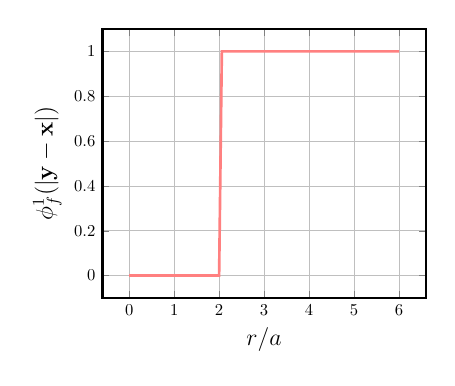
\begin{tikzpicture}[scale=0.6]
    \begin{axis}[
        xlabel={\Large$r/a$},
        ylabel={\Large$\phi_f^1(|\textbf{y}-\textbf{x}|)$},
        legend style={at={(0.05,0.05)}, anchor=south west},
        grid=major,
        domain=0:6,
        samples=100,
        ultra thick
    ]
    
    % Plot for phi = 0.05
    \addplot[color=red!50,ultra thick]
    { x < 2 ? 0 : 1};
    % \addlegendentry{$\phi = 0.05$}
    
    % % Plot for phi = 0.01
    % \addplot[color=blue!50,ultra thick]
    % { exp(-0.01 * (x^3 - 1))};
    % \addlegendentry{$\phi = 0.01$}
    
    % % Plot for phi = 0.001
    % \addplot[color=green!50,ultra thick]
    % { exp(-0.0001 * (x^3 - 1))};
    % \addlegendentry{$\phi = 10^{-4}$}
    
    \end{axis}
\end{tikzpicture}


In that case we must treat the problem into three region 
\paragraph*{First : $|\textbf{y} - \textbf{x}| > 2a$ :} we have $\phi_f^1 = \phi_f$, thus, $\phi_f^{1d} = 0$. same for $\phi_d$
\begin{align*}
    \avg{(\delta_1 - P_1)\rho^0\textbf{w}}
    &=0\\
    \avg{(\delta_1 - P_1)\rho^0\textbf{u}^0} / P_1
    &= 
    % \avg{(\delta_1 - P_1)\rho_f\chi_f\textbf{u}^0_f}
    % \avg{(\delta_1 - P_1)\rho_d\chi_d\textbf{u}^0_d}
    % = 
    \rho_f\phi_f\textbf{u}^{1d}_f
    + 
    \rho_d\phi_d\textbf{u}^{1d}_d
    \\
    \avg{(\delta_1 - P_1)\bm\sigma^0} 
    &= 
    - \phi_f^1 p^{1d}_f\bm\delta P_1 
    +\mu_f P_1 (\grad \textbf{u}^{1d} + \grad \textbf{u}^{1d})
    + \avg{(\delta_1 - P_1) \chi_d\bm\sigma^0_d}
\end{align*}
My guess is $\rho_f\phi_f\textbf{u}^{1d}_f
+ 
\rho_d\phi_d\textbf{u}^{1d}_d = \textbf{u}^{1d}$ 

and indeed we have 
\begin{equation*}
    \avg{\delta_1\textbf{u}^0} - \textbf{u}P_1
    = \avg{\delta_1 \chi_f \textbf{u}_f^0 + \chi_d \textbf{u}_d^0\delta_1 }
    - \textbf{u}_f\phi_fP_1
    - \textbf{u}_d\phi_dP_1
    \approx
    \phi_f^1 \textbf{u}_f^{1d} 
    + \phi_d^1 \textbf{u}_d^{1d}
\end{equation*}

\subsubsection*{Computation of the fluid phase term}

For suspension of spherical particles in the dilute limit the fluid phase averaged fields may be simplyfied by noticing that $\phi_f^1[\textbf{x},t;\textbf{y},\textbf{c}] P_1[\textbf{y},\textbf{c},t] = P_1[\textbf{y},\textbf{c},t]$ when $|\textbf{x} - \textbf{y}| > a$. 
\begin{equation}
    \avg{\chi_f f_f^0}[\textbf{x},t]
    = 
    \int_{\mathbb{R}^3}
    \int_{\mathbb{R}^3}
    f_f^1 \phi_f^1[\textbf{x},t;\textbf{y},\textbf{c}] P_1[\textbf{y},\textbf{c},t]
    d\textbf{y} 
    d\textbf{c}
\end{equation}
where,
\begin{equation*}
    f_f^1 \phi_f^1[\textbf{x},t;\textbf{y},\textbf{c}] P_1[\textbf{y},\textbf{c},t]
    =     
    \int
    \frac{1}{N}
    \sum_\alpha \delta(\textbf{y}-\textbf{x}_\alpha)
     \delta(\textbf{c}-\textbf{u}_\alpha)
    \chi_f
    f^0_f[\textbf{x},t;\FF]
    d\PP.
\end{equation*}

% \section{Introduction}
\label{ap:Closure_problem}

The equations governing the closure problem are often derived based on physical principles or intuitive reasoning.
For example, to determine the drag force term in the averaged momentum equation, in the dilute limit, the problem of a translating sphere in an unbounded flow with background velocity $\textbf{u}^\infty$ is commonly considered \citep{stone2001inertial,raja2010inertial,guazzelli2011}.
"background velocity" refers to the undisturbed flow at the particle location as if the particle were not present.


However, in the context of averaged equations, one might wonder: does $\textbf{u}^\infty$ correspond to the averaged fluid velocity $\textbf{u}_f$ (as used in \citet{jackson1997locally,zhang1997momentum}), the bulk velocity $\textbf{u}$ \citep{kim1985modelling}, or the Favre-averaged velocity $\textbf{u}_m$?
In other words, how can we relate the ensemble-averaged properties of the "hybrid" or "two-fluid" model to the closure terms?

As demonstrated, this question introduces the need for a rigorous statistical derivation of the closure problem.

The closure terms in the ``Hybrid'' model are the results of the ensemble average operator $\avg{\ldots}$. 
In all rigor, we cannot compute theoretically such an average since it necessitates knowing the distribution $P(\FF)$ and the exact expression of the local terms indicated by the notation $(\ldots)^0$. 
In the same spirit as in \citet{buyevich1979flow,lhuillier1992ensemble,batchelor1972sedimentation,hinch1977averaged} and \citet{zhang1994averaged} we demonstrate here that it is therefore necessary to reformulate the closure term to remove the ensemble average procedure. 
We demonstrated in \ref{ap:Closure_problem} that any ensemble-averaged quantities can be reformulated as an integral of what we call \textit{conditionally-averaged quantities}. 
The expressions obtained are  consistent with \citet{batchelor1972sedimentation,hinch1977averaged} and \citet[Appendix A]{zhang1994averaged} which also proposed conditional averages, but somewhat more general because our methodology applies to any closure term of the ``Hybrid model''. 
In a second step, we demonstrate how to derive what we call the \textit{conditionally-averaged equations} that are needed to obtain the \textit{conditionally-averaged quantities}. 

In the limit of Stokes flows \citet{hinch1977averaged} were the first authors to introduce this methodology.
He used the \textit{conditionally-averaged equations} to re-demonstrate, as a proof of concept, the bulk stress of a suspension of solid spheres at $\mathcal{O}(\phi^2)$ and the sedimentation velocity of the dispersed phase at $\mathcal{O}(\phi^2)$. 
In \citet{kim1985modelling} they use the \textit{conditionally-averaged equations} to consider the effect of finite volume fraction on the drag force closure term, in fixed beds of spherical solid spheres, their analysis holds for arbitrary volume fraction $\phi$. 

Again our derivation is directly inspired by the cited author, but the approach is generalized by considering fluid inclusion and an inertial regime. 
For instance, in the dilute regime, the \textit{conditionally-averaged equations} correspond to the problem of the disturbance field generated by an isolated translating droplet. 
The real interest behind this demonstration is that it is kept general and offers many possibilities for model extension.
 




% In \ref{sec:reformulation} and \ref{sec:the_disturbance_eq} we discuss the general approach to derive the closure problem
%%%%%%%%%%%%%%%%%%% A mettre dans lautre chap
% , while in \ref{sec:application} we derive the closures terms of the momentum and energy equations. 
% Since the derivation of the closure terms can be understood through physical arguments, readers who are less interested in the rigorous mathematical formulation of the closure problem, which can be quite involved, may skip directly to \ref{sec:application}.


\section{Reformulation of the closure terms}
\label{sec:reformulation}

% We aim to compute our closures within the dilute Stokes flow regime for spherical particles of radius $a$. 
% In this regime we expect that the closure terms will only be determined by the center of mass velocity of the droplets ($\textbf{u}_p$), their position in space, and the macroscopic properties of the continuous phase ($\textbf{u}_f, \grad \textbf{u}_f \ldots$). 
% Indeed, as we will demonstrate in the following section, only these properties define the boundaries of the \textit{single-particle} conditionally-averaged equations, and are therefore sufficient to achieve closure of the problem  in the Stokes flow regime. 

In the following, we express our closures in terms of averaged quantities, conditioned on the position of the center of mass of a \textit{test-particle} and its center of mass velocity. 
Note that for shape-dependent closure terms it would also be necessary to obtain the \textit{shape-conditioned} averaged fields, but this is out of the scope of this work.
Similarly, to account for the contribution of droplet acceleration to the closure terms (such as the added mass effect), it would be necessary to consider the \textit{center-of-mass-acceleration-conditioned} averaged fields.
However, this lies beyond the scope of the present work.
  
\subsection{Interfacial terms}

In the equations presented in \ref{sec:application} certain closures, such as surface stresses and surface heat fluxes, are expressed in the form of particle-averaged surface integrals. 
Here, we focus on reformulating these terms in terms of \textit{single-particle} conditionally-averaged quantities, which will be defined in the subsequent sections.

As the procedure is similar for all surface particle-averaged terms, let us take the example of the exchange of momentum term appearing in the continuous and dispersed phase averaged momentum equations (\ref{eq:dt_hybrid_rhou_f} and \ref{eq:dt_hybrid_up}). 
From the definition of the particle average we write,
\begin{align}
    \pSavg{\bm\sigma_f^0\cdot\textbf{n}}[\textbf{x},t]
    &= \avg{ \sum_{\alpha=1}^N \delta(\textbf{x}-\textbf{x}_\alpha[t; \FF])
    \int_{\Gamma_\alpha(t,\FF)}
    (\bm\sigma_f^0\cdot\textbf{n})[\textbf{y},t;\FF]
    d\Gamma[\textbf{y}] }
    \label{eq:first_step_reallay}
\end{align}
By writing this integral explicitly, we emphasize that the particle-averaged quantity (left-hand side of \ref{eq:first_step_reallay}) is evaluated at the point \textbf{x}, while the parameter $\textbf{y}$ is used for the integration over the particle's surface.
Recall that $\Gamma_\alpha$ refers to the surface of the droplet $\alpha$ and $\textbf{x}_\alpha$ to the position of the center of mass of that same droplet $\alpha$. 
Thus, the notation $(\bm\sigma_f^0\cdot\textbf{n})[\textbf{y},t;\FF]$ means that we evaluate the local stress as well as the local normal $\textbf{n}$ to the particle surface, at \textbf{y}. 
We now enlarge the domain of integration from $\Gamma_\alpha$ (the surface of the particle $\alpha$) to $\mathbb{R}^3$ with the introduction of the interface indicator function of the particle $\alpha$, namely $\delta(|\textbf{y} - \textbf{x}_\alpha[t,\FF]| - a)$\footnote{Indeed, for spherical particles, we can define the interface indicator function of a single particle using the definition $\delta_\Gamma = \delta(|\textbf{y} - \textbf{x}_\alpha[t,\FF]| - a)$.}. 
It reads,
\begin{multline}
    \pSavg{\bm\sigma_f^0\cdot\textbf{n}}[\textbf{x},t]
    = \\
    \int_{\mathbb{R}^3}
    \avg{
     \sum_{\alpha=1}^N 
     \delta(\textbf{x}-\textbf{x}_\alpha[t \FF])
    \delta(|\textbf{y} - \textbf{x}_{\alpha}[t;\FF]|-a)
    (\bm\sigma_f^0\cdot\textbf{n})[\textbf{y},t;\FF]
    }
    d\textbf{y}. 
    \label{eq:first_step_drag}
\end{multline} 
Since the domain of integration $\mathbb{R}^3$ is now independent of $\FF$, we may substitute the integral and ensemble average operator. 

As mentioned above, we assume that the closure terms are entirely determined by the center of mass velocity of the particles and their position in space. 
Therefore, to include the condition on the particle velocity we introduce the relation 
\begin{equation}
    \int_{\mathbb{R}^3} \delta(\textbf{w} - \textbf{u}_\alpha[\FF,t]) d\textbf{w} = 1,
    \label{eq:Pw_normed}
\end{equation}
where $\textbf{w}$ is the test-particle center of mass velocity in the Eulerian space and $\textbf{u}_\alpha$ is the center of mass velocity within the Lagrangian framework. 
Injecting \ref{eq:Pw_normed} into \ref{eq:first_step_drag} one obtains, 
\begin{multline}
    \pSavg{\bm\sigma_f^0\cdot\textbf{n}}[\textbf{x},t]
    = \\
    \int_{\mathbb{R}^3}
    \int_{\mathbb{R}^3}
    \avg{
     \sum_{\alpha=1}^N 
     \delta(\textbf{x}-\textbf{x}_\alpha[t \FF])
     \delta(\textbf{w} - \textbf{u}_\alpha[\FF,t])
    \delta(|\textbf{y} - \textbf{x}_{\alpha}[t;\FF]|-a)
    (\bm\sigma_f^0\cdot\textbf{n})[\textbf{y},t;\FF]
    }
    d\textbf{y}
    d\textbf{w}. 
    \label{eq:second_step_drag}
\end{multline}
The quantity with the ensemble average operator now represents the average of the local stress $(\bm\sigma_f^0\cdot\textbf{n})[\textbf{y},t;\FF]$ on every configuration where the interface of a droplet is present at \textbf{y} with its center of mass at \textbf{x} and with a center of mass velocity \textbf{w}.


Moreover, since the expression within the ensemble average in \ref{eq:first_step_drag} is identically zero when, $\textbf{x}_\alpha \neq \textbf{x}$, we may replace the interface indicator function such that 
\begin{equation}
    \delta(\textbf{x}-\textbf{x}_\alpha[t,\FF])\delta(|\textbf{y} - \textbf{x}_{\alpha}[t,\FF]|-a) = \delta(\textbf{x}-\textbf{x}_\alpha[t,\FF])\delta(|\textbf{y} - \textbf{x}|-a). 
    \label{eq:from_R3_to_S}
\end{equation}
Since the function $\delta(|\textbf{y} - \textbf{x}|-a)$ is not dependent on $\FF$ it can be taken out of the ensemble average operator, hence reducing the domain of integration from $\mathbb{R}^3$ to $|\textbf{y}-\textbf{x}| = a$ in \ref{eq:first_step_drag}. 
\footnote{For deformable or non-spherical particles, this function may take a more complicated form, since the interface of a deformable or anisotropic particle is not entirely determinate by its center of mass position. 
It is clear that if the position of the interface is conditioned by the exact shape of the interface, then we can always express the interface indicator function as $\delta(f(\textbf{x}))$ where $f$ is a distance function of the shape that may depend on the particle's orientation (for anisotropic particles) or aspect ratio (for slightly deformable ones). 
Anyhow, this approach is generalizable to other kinds of particles, but in this work, we consider only spherical droplets. 
Note that for spheroidal particles as in \ref{chap:deformable} we may write $\delta_{\alpha\Gamma} = \delta((\textbf{y} - \textbf{x}_\alpha[t,\FF])\cdot (\bm\chi_\alpha+\bm\delta)\cdot(\textbf{y} - \textbf{x}_\alpha[t,\FF]) - a^2)$ where we have used the notation of \ref{chap:deformable}
}

Injecting \ref{eq:from_R3_to_S} into \ref{eq:second_step_drag} and using the last remark leads us to the relation 
\begin{equation}
    \pSavg{\bm\sigma_f^0\cdot\textbf{n}}[\textbf{x},t]
    =
    \int_{\mathbb{R}^3}
    P_1[\textbf{x},\textbf{w},t]
    \int_{|\textbf{x}-\textbf{y}|=a}
    (\bm\sigma_f^1 \cdot \textbf{n})[\textbf{y},\textbf{x},\textbf{w},t]
    d\textbf{y}
    d\textbf{w}
    \label{eq:conditionally_averaged}
\end{equation}
where we introduced the definitions, 
\begin{align}
    \bm\sigma^1_f[\textbf{y},\textbf{x},\textbf{w},t]
    % \phi_I^1[\textbf{y}|\textbf{x},\textbf{w},t] 
    % P_1[\textbf{x},\textbf{w},t]
    &= 
    \frac{1}{P_1}
    \avg{
    \sum_\alpha^N 
    \delta(\textbf{x} - \textbf{x}_\alpha[t,\FF])
    \delta(\textbf{w} - \textbf{u}_\alpha[t,\FF])
    % \delta(|\textbf{y} - \textbf{x}_{\alpha}[t,\FF]|-a)
    \bm\sigma_f^0[\textbf{y},t,\FF]
    },
    \label{eq:sigma_f_1}
    \\
    % \phi_I^1[\textbf{y}|\textbf{x},\textbf{w},t] 
    % P_1[\textbf{x},\textbf{w},t]\nonumber\\
    % = 
    % \avg{
    % \sum_\alpha^N 
    % \delta(\textbf{x} - \textbf{x}_\alpha[t,\FF])
    % \delta(\textbf{w} - \textbf{u}_\alpha[t,\FF])
    % \delta(|\textbf{y} - \textbf{x}_{\alpha}[t,\FF]|-a)
    % }\\
    P_1[\textbf{x},\textbf{w},t]
    &= 
    \avg{
    \sum_\alpha^N 
    \delta(\textbf{x} - \textbf{x}_\alpha[t,\FF])
    \delta(\textbf{w} - \textbf{u}_\alpha[t,\FF])
    }. 
\end{align}
% \tb{Since we reduced the surface int the stress isn't any more conditioned by the surface }
% Here $\bm\sigmais the \textit{single-particle} conditionally-averaged local stress of the continuous phase knowing that interface of the particle at $\textbf{x}$ is  present in \textbf{y} and that there is a particle at \textbf{x} with velocity \textbf{w}. 
With this definition, $\bm\sigma^1_f$ is the continuous phase stress, evaluated at $\textbf{y}$ and time $t$, knowing that there is a particle at position $\textbf{x}$ with velocity \textbf{w}, and that the point \textbf{y} is occupied by the surface of the test-particle 
\footnote{
    As $\bm\sigma^1_f$ is conditioned on the variables: $\textbf{y}$, $\textbf{x}$, $\textbf{w}$, $t$, and evaluated at the position $\textbf{y}$ and time $t$, we should write: $\bm\sigma^1_f[\textbf{y},t|\textbf{x},\textbf{y},\textbf{w},t]$ instead of $\bm\sigma^1_f[\textbf{x},\textbf{y},\textbf{w},t]$.
    However the second notation will be used as a short hand. 
}.
% $\phi_I^1[\textbf{y}|\textbf{x},\textbf{w},t] $ is the probability of finding the interface of the particle at the location \textbf{y} knowing its center of mass is located at \textbf{x}. 
% For identical spherical particles we can write $\phi_I^1[\textbf{y}|\textbf{x},\textbf{w},t] = \delta(|\textbf{x} - \textbf{y}| -a)$.
% That is why the domain of integration over \textbf{y} in \ref{eq:conditionally_averaged} is reduced to $|\textbf{x} - \textbf{y}| < a$. 
$P_1[\textbf{x},\textbf{w},t]$ is the probability of finding a particle center of mass at \textbf{x} with velocity \textbf{w} at time $t$.
This distribution can be decomposed such that $P_1[\textbf{x},\textbf{w},t] = n_p[\textbf{x},t] P_1[\textbf{w}|\textbf{x},t]$ where $n_p$ is the number density evaluated at \textbf{x}, and $P_1$ the probability density of having a particle with velocity \textbf{w} knowing its center of mass location is \textbf{x}. 
Note that this distribution is normed 
\begin{equation*}
    \int_{\mathbb{R}^3} P_1[\textbf{w}|\textbf{x},t] d \textbf{w} = 1. 
\end{equation*}
Finally, note that in \ref{eq:conditionally_averaged} the droplet shape and the position of its center of mass fully determine the normal vector $\textbf{n}$, allowing it to be taken outside the ensemble average. 


\subsubsection{Single-particle conditionally averaged quantities}

All quantities denoted with the superscript $^1$ refer to \textit{single-particle} conditionally-averaged quantities. 
These quantities are conditionally averaged based on the presence of a particle located at \textbf{x} with velocity \textbf{w}.
Additionally, in the following, we will use the shorthand,
\begin{equation}
    \delta_1[\textbf{x},\textbf{w},t,\FF]  \text{ for } \sum_\alpha \delta(\textbf{x} - \textbf{x}_\alpha[t,\FF]) \delta(\textbf{w} - \textbf{u}_\alpha[t,\FF]). 
    \label{eq:delta_1}
\end{equation}  
Thus, we can define the \textit{single-particle} conditional-average of a local quantity $f^0$, as 
\begin{equation}
    f^1[\textbf{y}|\textbf{x},\textbf{w},t] P_1[\textbf{x},\textbf{w},t] = \avg{\delta_1 f^0[\textbf{y},\FF,t]}.
\end{equation}
Such that $f^1$ is the averaged value of $f^0$ at \textbf{y} knowing that there is a particle at \textbf{x} with velocity \textbf{w}. 
If $f_k$ is a quantity defined in the phase $k$ we may write 
\begin{equation*}
    f^1_k[\textbf{y}|\textbf{x},\textbf{w},t] \phi_k^1[\textbf{y}|\textbf{x},\textbf{w},t]  P_1 = \avg{\delta_1 (\chi_k f^0_k) [\textbf{y},\FF,t]}.
\end{equation*}
Such that $\phi_k^1$ is the probability of finding the phase $k$ at \textbf{y} knowing a particle is located at \textbf{w} with velocity \textbf{w}, and $f_k^1$ the conditional average of $f_k^0$. 
For example, we define the \textit{single-particle conditioned average} of the continuous phase velocity fields by, 
\begin{equation*}
    \textbf{u}_f^1 \phi_f^1 P_1
    = \avg{\delta_1 \chi_f \textbf{u}_f^0}
\end{equation*} 
where $\phi_f^1$ is the probability of finding the continuous phase at \textbf{y} knowing a particle is present at \textbf{x} with velocity \textbf{w}. 
$\textbf{u}_f^1$ is the averaged local velocity evaluated at \textbf{y} knowing the continuous phase is present at \textbf{y} with a particle at \textbf{x} having velocity \textbf{w}. 

The stress present in \ref{eq:conditionally_averaged} can now be expressed in terms of conditionally-averaged velocity and pressure fields. 
We use the constitutive law of Newtonian fluids, $\bm\sigma_f^0 = -p_f^0 \bm\delta + \mu_f [\pddy \textbf{u}_f^0+ (\pddy \textbf{u}_f^0)^\dagger]$, with $\pddy$ the gradient over the \textbf{y} coordinate.
Injecting this law into \ref{eq:sigma_f_1} we obtain directly 
\begin{equation}
    \bm\sigma_f^1
    = - p_f^1 \bm\delta
    +\mu_f [\pddy \textbf{u}_f^1+(\pddy \textbf{u}_f^1)^\dagger], 
    \label{eq:sigma_f_surf}
\end{equation}
since $\delta_1$ is independent of \textbf{y}, meaning that it could be permuted with the gradient operator in \ref{eq:sigma_f_surf}. 
Note that this relation is valid only because $\bm\sigma_f^1$ is conditioned on the presence of an interface at \textbf{y} in \ref{eq:sigma_f_1}. 
In conclusion, the ensemble averaged exchange of momentum term can be expressed as the surface integral of the Newtonian stress defined based on the \textit{single-particle} conditional-averaged fields: $\textbf{u}_f^1$, and $p_f^1$. 

It must be understood that this definition \eqref{eq:sigma_f_surf} is only true because the stress is evaluated at the surface of the droplet, in the general case we have, 
\begin{equation}
    P_1 \phi_f^1 \bm\sigma_f^1
    =
    \avg{\delta_1 \chi_f \bm\sigma_f^0}
    =
    P_1 \phi_f^1 p_f^1
    +  \avg{\delta_1\chi_f \{ - p_f^0 \bm\delta + \mu_f [\pddy \textbf{u}_f^0+  (\pddy \textbf{u}_f^0)^\dagger]\}}. 
    \label{eq:sigme_f_1_all_space}
\end{equation}
Note the presence of $\chi_f$ in this expression, in opposition to \ref{eq:sigma_f_surf} where only $\delta_1$ where present.
This is because \ref{eq:sigme_f_1_all_space} is evaluated at an arbitrary point \textbf{y}, while in \ref{eq:sigma_f_surf} we consider only the points lying on the droplet interface.  
From this expression, we can propose two formulations for the continuous phase stress,   
\begin{align}    
    \bm\sigma_f^1
    &= 
    - p_f^1 \bm\delta 
    + \mu_f [\pddy \textbf{u}_f^1+ (\pddy \textbf{u}_f^1)^\dagger ]
    - \frac{\mu_f }{P_1 \phi_f^1}\avg{\delta_1 \delta_\Gamma (\textbf{n}_d \textbf{u}_f''+  \textbf{u}_f'' \textbf{n}_d)},
    \label{eq:sigma_f_surf15}
    \\
    \bm\sigma_f^1
    &= 
    - p_f^1 \bm\delta 
    + \frac{\mu_f }{\phi_f^1} [\pddy \textbf{u}^1+ (\pddy \textbf{u}^1)^\dagger ]
    - \frac{\mu_f }{\phi_f^1} \phi_d^1 \textbf{e}_d^1. 
    \label{eq:sigma_f_surf2}
\end{align}
Where we have defined $\textbf{u}_f'' = \textbf{u}_f^0 - \textbf{u}_f^1$. 
These two expressions can be derived using a similar methodology than for the derivation of \ref{eq:second_form,eq:first_form}. 
Note that the second term on the right-hand side of \ref{eq:sigma_f_surf2} vanishes for solid particles, the rate of strain within solid particle is null.
While the second term of \ref{eq:sigma_f_surf15} does not necessarily vanish. 
That is why the second expression is preferred for solid particles. 

% Additionally, multiplying \ref{eq:sigma_f_surf15} and \ref{eq:sigma_f_surf2} by $\phi_f^1$ and subtracting both expressions gives, 
% \begin{equation} 
%     \frac{1}{P_1}\avg{\delta_1 \delta_\Gamma (\textbf{n}_d \textbf{u}_f''+  \textbf{u}_f'' \textbf{n}_d)}
%     -  \phi_d^1 \textbf{e}_d^1
%     = 
%     [(\textbf{u}_f^1 - \textbf{u}_d^1)\pddy\phi_d^1+ \pddy \phi_d^1(\textbf{u}_f^1 - \textbf{u}_d^1) ]
%     - \phi_d^1 [\pddy\textbf{u}_d^1+  (\pddy \textbf{u}_d^1)^\dagger ]. 
% \end{equation}
% For ensemble averaged (not conditionally-averaged) quantities we can equally show that
% \begin{multline} 
%     \avg{\delta_\Gamma (\textbf{n}_d \textbf{u}_f'+  \textbf{u}_f' \textbf{n}_d)}
%     - \phi_d \textbf{e}_d
%     = 
%     +  [(\textbf{u}_f - \textbf{u}_d)\pddy\phi_d+ \pddy \phi_d(\textbf{u}_f - \textbf{u}_d) ]
%     - \phi_d [\pddy\textbf{u}_d+  (\pddy \textbf{u}_d)^\dagger ]
% \end{multline}
% Note that for solid particles this relation can directly lead us to a closure for the surface term on the left-hand side, namely
% \begin{multline} 
%     \avg{\delta_\Gamma (\textbf{n}_d \textbf{u}_f'+  \textbf{u}_f' \textbf{n}_d)}
%     = 
%     [(\textbf{u}_f - \textbf{u}_d)\pddy\phi_d+ \pddy \phi_d(\textbf{u}_f - \textbf{u}_d) ]
%     - \phi_d [\pddy\textbf{u}_d+  (\pddy \textbf{u}_d)^\dagger ]. 
%     \label{eq:closure_un_nu}
% \end{multline}

\begin{figure}[h!]
    \centering
    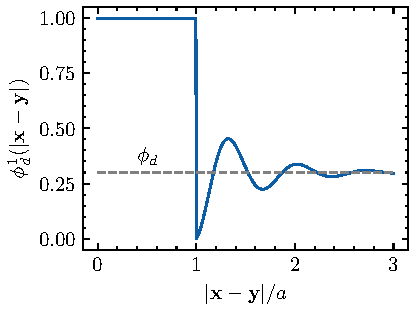
\includegraphics[width=0.2\textheight]{image/dist_phi.pdf}
    \caption{Representation of a possible form for the probability of finding the dispersed phase at \textbf{x} knowing a spherical particle of radius $a$ is present at $\textbf{y}$.
    Note the zone empty of particle concentration near the points $|\textbf{x}- \textbf{y}|=a$, this due to the impenetrability of particles. 
    }
    \label{fig:distrib}
\end{figure}
At the surface of the test-particle, the probability of finding the dispersed phase, i.e. finding the dispersed phase in contact with the surface of the reference particle, is identically null (not to be confused with the probability of finding another droplet center of mass). 
Indeed, a thin film of continuous phase always separates the droplet surface from its neighbors (see \ref{fig:distrib}).
Therefore, we may write $\phi_d^1 = 0$ at $|\textbf{x}- \textbf{y}| =a$. 
Thus, when evaluated at the subsurface of the particle, we can use the relation $\textbf{u}_f^1 = \textbf{u}^1$ and $p_f^1 = p^1$. 
Consequently, to compute the surface stress of a particle, either the conditionally-averaged quantities of the continuous phase ($\textbf{u}_f^1, p_f^1$) or the bulk quantities ($\textbf{u}^1$, $p^1$) are required. 
Another consequence of this is that, the definitions given by, \ref{eq:sigma_f_surf15}, \ref{eq:sigma_f_surf2}, or \ref{eq:sigma_f_surf} are all consistent when evaluated at the points located on the surface of the droplet at \textbf{x}. 

\subsection{Mean fields and disturbance fields contribution}

As it is often done in the literature \citep{zhang1994ensemble,jackson2000,wang2021numerical,wang2024effect}, we would like to separate the averaged momentum exchange into a contribution from the mean flow and pressure fields, and the contribution arising due to the disturbance velocity and pressure fields.  

\subsubsection{Definitions}

In the first place, we need to define what is a disturbance field.
Let us take the example of the conditioned velocity field, $\textbf{u}_f^1$, and its corresponding disturbance velocity field.
We state that the conditioned field, $\textbf{u}_f^1$, is equivalent to the ensemble-averaged velocity field $\textbf{u}_f$ when the particle at \textbf{x} is sufficiently far from the point where the velocity $\textbf{u}_f^1$ is evaluated (the point \textbf{y}).
Thus, we write,  
\begin{equation}
    \lim_{|\textbf{y}-\textbf{x}|\to\infty} 
    \textbf{u}_f^1[\textbf{y},\textbf{x},\textbf{w},t]
    =
    \textbf{u}_f[\textbf{y},t]. 
    \label{eq:lim_u_1}
\end{equation} 
Note that this definition requires an infinitely large domain. 
This implies that the solutions obtained in the subsequent sections are restricted to infinitely large domains, devoid of boundary conditions.

Let us assume that $L$ is the macroscopic length scale of our process and that $a$  is the typical size of the particles.
Since the particle-size scale $a$ is much smaller than the boundary length scale $L$ we assume that $\textsc{O}(a/L)$ is negligible. 
In the worth case scenario, the disturbance field of a droplet is $(\textbf{u}_f^1- \textbf{u}_f)\sim a/|\textbf{y}-\textbf{x}|$ \citet{kim2013microhydrodynamics}.
Hence, in a physical situation where $|\textbf{y}-\textbf{x}|\to L$ instead of $|\textbf{y}-\textbf{x}|\to\infty$ in \ref{eq:lim_u_1} we may estimate that the error is of $\mathcal{O}(a/L)$, hence negligible upon a reasonable separation of scale.
However, it is interesting to note that this will no longer be the case for other problems such as sediment transport for examples.
In this case, the boundary condition, i.e. the top of the particle bed and the ground, are at a distance of the same length scale as the particle-size. 

In light of \ref{eq:lim_u_1}, we define the disturbance velocity field as 
\begin{equation}
    \textbf{u}_f^{1d}
    =
    \textbf{u}_f^1 
    - 
    \textbf{u}_f. 
    \label{eq:def_u_1d}
\end{equation}
because it satisfies the definition, 
\begin{equation}
    \lim_{|\textbf{y}-\textbf{x}|\to\infty} 
    \textbf{u}_f^{1d}[\textbf{y},\textbf{x},\textbf{w},t]
    =
    \lim_{|\textbf{y}-\textbf{x}|\to\infty} 
    \{\textbf{u}_f^1[\textbf{y},\textbf{x},\textbf{w},t]
    - \textbf{u}_f[\textbf{y},t]\}
    = 0.
    \label{eq:lim_u_1d}
\end{equation} 
Thus, $\textbf{u}_f^{1d}$ tends to zero at large distances from the particle, which is consistent with the terminology ``disturbance''.
The definition \ref{eq:def_u_1d} can apply to any \textit{conditional-averaged} quantities $f^1$, we define
\begin{equation}
    \lim_{|\textbf{y}-\textbf{x}|\to\infty} 
    \{f_f^1[\textbf{y},\textbf{x},\textbf{w},t]
    - f_f[\textbf{y},t]\}
    =
    f_f^{1d}[\textbf{y},\textbf{x},\textbf{w},t]
    = 0.
\end{equation} 

\subsubsection{Momentum exchange decomposition}

Using the decomposition $\bm\sigma_f^1 = \bm\sigma_f^{1d} + \bm\sigma_f$ in \ref{eq:conditionally_averaged} we finally introduce the decomposition of the averaged momentum exchange term as:  
\begin{align}
    \pSavg{\bm\sigma_f^0\cdot\textbf{n}}[\textbf{x},t]
    =
    n_p[\textbf{x},t]
    \int_{|\textbf{x}-\textbf{y}|=a}
    \bm\sigma_f[\textbf{y},t]
    \cdot \textbf{n}
    d\textbf{y}
    \nonumber
    \\
    + 
    \int_{\mathbb{R}^3}
    P_1[\textbf{x},\textbf{w},t]
    \int_{|\textbf{x}-\textbf{y}|=a}
    \bm\sigma_f^{1d}[\textbf{y},\textbf{x},\textbf{w},t]
    \cdot \textbf{n}
    d\textbf{y}
    d\textbf{w}
    \label{eq:general_partition}
\end{align}
where the first term represents the contribution from the mean continuous phase stress, $\bm\sigma_f$, and the second term is the contribution from the disturbance fields stress $\bm\sigma_f^{1d}$. 
While this decomposition is arbitrary since $\bm\sigma_f^1$ could be partitioned into other arbitrary tensors, it enables by definition, the separation of the mean flow contribution, $\bm\sigma_f$, from the stress induced by the local-scale disturbance fields, $\bm\sigma_f^{1d}$.
This decomposition is used by \citet[Chapter 2]{jackson2000} and \citet{zhang1997momentum,wang2021numerical,wang2024effect} for suspensions of solid spheres, although these authors do not explicitly provide the expression for the tensor $\bm\sigma_f^{1d}$, which we aim to derive in the following sections. 

Note that $\bm\sigma_f$ is evaluated at $\textbf{y}$ in \ref{eq:general_partition}. 
Although $\bm\sigma_f$ is ensemble-averaged, we emphasize that it may still depend on the position in inhomogeneous flows. 
Assuming the suspension is slightly non-homogeneous \citep{lhuillier1992ensemble}, we have $\bm\sigma_f[\textbf{y},t] = \bm\sigma_f[\textbf{x},t] + \textbf{r}\cdot \nabla\bm\sigma_f[\textbf{x},t] + \ldots$, where $\textbf{r} = \textbf{y} - \textbf{x}$. 
By retaining only the first three terms in the expansion, we can demonstrate that
\begin{equation}
    \pSavg{\bm\sigma_f^0\cdot\textbf{n}}
    =
    n_p v_p 
    \div\bm\sigma_f
    +
    \int_{\mathbb{R}^3}
    P_1
    \int_{|\textbf{x}-\textbf{y}|=a}
    \bm\sigma_f^{1d} \cdot \textbf{n}
    d\textbf{y}d\textbf{w}.
    \label{eq:drag_final}
\end{equation}
Therefore, the total momentum exchange term contains a component related to the divergence of the mean fluid-phase stress, in addition to the contribution from the disturbance fields. 
Similar arguments can be extended to the first two moments of the hydrodynamic force. 
These expressions can be written as:
\begin{align}
    \pSavg{\textbf{r}\bm\sigma_f^0\cdot\textbf{n}}
    &=
    n_p v_p \bm\sigma_f
    +
    \int_{\mathbb{R}^3}
    P_1
    \int_{|\textbf{x}-\textbf{y}|=a}
    \textbf{r}\bm\sigma_f^{1d} \cdot \textbf{n}
    d\textbf{y}
    d\textbf{w},
    \label{eq:first_mom_general}
    \\
    \pSavg{\textbf{rr}\bm\sigma_f^0\cdot\textbf{n}}
    &=
    n_pv_p  \frac{a^2}{5} 3 [(\div \bm\sigma_f)\bm\delta]^\text{sym}
    +
    \int_{\mathbb{R}^3}
    P_1
    \int_{|\textbf{x}-\textbf{y}|=a}
    \textbf{rr}\bm\sigma_f^{1d} \cdot \textbf{n}
    d\textbf{y}
    d\textbf{w},
    \label{eq:second_mom_general}
\end{align}
where the operator $[\ldots]^\text{sym}$ returns the symmetric part of the arguments. 
It is important to note that the contribution from the mean stress in the second moment of the hydrodynamic force may become negligible when a proper separation of scale is considered. 
Indeed, this term is proportional to $a^2$ \eqref{eq:second_mom_general}, and it appears under the operator $\grad\grad\sim L^{-2}$ in the averaged momentum equation \ref{eq:dt_hybrid_rhou_f}, hence contributing to $\mathcal{O}(a^2/L^2)$, which may be considered as negligible. 

According to the expressions \ref{eq:drag_final}, \ref{eq:first_mom_general}, and \ref{eq:second_mom_general}, we will need to compute the term $\bm\sigma^{1d}_f = \bm\sigma_f^1 - \bm\sigma_f$ where $\bm\sigma_f^1$ is given by \ref{eq:sigma_f_surf}. 
Regarding the mean continuous phase stress we recall that it can be written in two ways (see \ref{chap:daniel15}), namely 
\begin{align}
    \label{eq:mean_continuous_phase_stress}
    \bm\sigma_f
    &= - p_f \bm\delta 
    + \mu_f [\pddy \textbf{u}_f+ (\pddy \textbf{u}_f)^\dagger ]
    - \frac{\mu_f}{\phi_f}\avg{\delta_\Gamma (\textbf{n}_d \textbf{u}_f'+  \textbf{u}_f' \textbf{n}_d)}, \\
    \bm\sigma_f
    &= - p_f \bm\delta 
    + \frac{\mu_f}{\phi_f} [\pddy \textbf{u}+ (\pddy \textbf{u})^\dagger ]
    - \frac{\mu_f \phi_d}{\phi_f} \textbf{e}_d
    \label{eq:mean_continuous_phase_stress2}
\end{align}
Thus using \ref{eq:sigma_f_surf} and \ref{eq:mean_continuous_phase_stress} we find for the points on the particle's surface ($|\textbf{y}-\textbf{x}| = a$) that,
\begin{align}
    \bm\sigma_f^{1d}
    =
    - p_f^{1d} \bm\delta 
    + \mu_f [\pddy \textbf{u}_f^{1d}+ (\pddy \textbf{u}_f^{1d})^\dagger ]
    + \frac{\mu_f }{\phi_f}\avg{\delta_\Gamma (\textbf{n}_d \textbf{u}_f'+  \textbf{u}_f' \textbf{n}_d)}. 
    \label{eq:sigma_explict}
\end{align}
Thus, according to \ref{eq:sigma_explict}, the disturbance stress that is integrated over the particle surface in \ref{eq:drag_final} to \ref{eq:second_mom_general}, is not only the Newtonian stress-like contribution of the disturbance fields ($\textbf{u}_f^1$ and $p_f^1$), but also includes the contribution of the term $\avg{\delta_\Gamma (\textbf{n}_d \textbf{u}_f'+  \textbf{u}_f' \textbf{n}_d)}$. 
Thus, in the force closures: \ref{eq:drag_final} and \ref{eq:first_mom_general}, we will observe the appearance of the terms involving the divergence of $\avg{\delta_\Gamma (\textbf{n}_d \textbf{u}_f'+  \textbf{u}_f' \textbf{n}_d)}$ times $n_pv_p$, and  $n_pv_p \avg{\delta_\Gamma (\textbf{n}_d \textbf{u}_f'+  \textbf{u}_f' \textbf{n}_d)}$, respectively. 
These terms will ultimately cancel out their corresponding contributions in $\bm\sigma_f$ that appear on the left-hand side of \ref{eq:drag_final} and \ref{eq:first_mom_general}. 

To provide a better understanding for the following discussion we remark that for solid particles $\textbf{e}_d = 0$. 
Therefore, subtracting \ref{eq:mean_continuous_phase_stress} from \ref{eq:mean_continuous_phase_stress2}, gives directly, 
\begin{equation}
    \avg{\delta_\Gamma (\textbf{n}_d \textbf{u}_f'+  \textbf{u}_f' \textbf{n}_d)}
    = 
    (\textbf{u}_f - \textbf{u}_d)\pddy \phi_d + \pddy \phi_d (\textbf{u}_f - \textbf{u}_d)
    -  \phi_d [\pddy \textbf{u}_d+ (\pddy \textbf{u}_d)^\dagger ]. 
    \label{eq:closure_un_nu}
\end{equation} 
Therefore, at least for solid particles, this term is non-zero as soon as there are non-negligible gradients of volume fraction and mean gradients of particle velocities. 


We conclude that the commonly used decomposition of the drag force introduced by \citet{zhang1997momentum,jackson2000}, given by \ref{eq:general_partition}, requires adding the term  $\avg{\delta_\Gamma (\textbf{n}_d \textbf{u}_f'+  \textbf{u}_f' \textbf{n}_d)}$ to the classical Newtonian stresses in the second term of \ref{eq:general_partition} and subtracting it in the mean drag force term (first term of \ref{eq:general_partition}). 
This finding implies that, in the recent work of \citet{wang2021numerical, wang2024effect}, where this decomposition is employed for the drag force, we assert that they have actually computed the integral of the first two terms of \ref{eq:sigma_explict}, while neglecting the final term. 
Interestingly, \citet{wang2024effect} specifically investigates the effect of the volume fraction gradient ($\grad \phi_d$) on the drag force. 
In this context, it is clear from \eqref{eq:closure_un_nu} that the term $\avg{\delta_\Gamma (\textbf{n}_d \textbf{u}_f'+  \textbf{u}_f' \textbf{n}_d)}$ cannot be neglected. 
Only when the analysis is accurate to $\mathcal{O}(\phi_d)$ does this term vanish in \ref{eq:drag_final}, reducing \ref{eq:sigma_explict} to the Newtonian stress expression. 
% Thus, the drag force computed in the DNS of \citet{wang2024effect} may not be the one defined in their momentum equations. 

Note that using \ref{eq:mean_continuous_phase_stress2} instead of \ref{eq:mean_continuous_phase_stress} in \ref{eq:sigma_explict} and switching $\textbf{u}_f^1$ and $\textbf{u}^1$ in \ref{eq:sigma_f_surf}, does not solve this inconsistency. 

\subsubsection{An alternative stress decomposition}

As the previous decomposition requires adding and subtracting $\avg{\delta_\Gamma (\textbf{n}_d \textbf{u}_f'+  \textbf{u}_f' \textbf{n}_d)}$ in each term of \ref{eq:general_partition}, we decide to avoid this overcomplicated operation and introduce, the partitioning 
\begin{equation}
    \bm\sigma_f^1 =
    \bm\Sigma_f + 
    \bm\Sigma_f^{1d}. 
    \label{eq:mean_Newtonian}
\end{equation}
Where the mean stress and disturbance stresses are defined as, 
\begin{align}
    \bm\Sigma_f^{1d}
    &=-p_f^{1d}\bm\delta + \mu_f^1 [\grad \textbf{u}^{1d}_f + (\grad \textbf{u}^{1d}_f)^\dagger], \\
    \bm\Sigma_f
    &=-p_f\bm\delta + \mu_f^1 [\grad \textbf{u}_f + (\grad \textbf{u}_f)^\dagger], 
\end{align}
respectively. 
Note that the use of $\textbf{u}_f$ as the ensemble-averaged velocity of reference is arbitrary.
Indeed, recall that at the surface of the test particle we have $\phi_d^1=0$, hence $\textbf{u}_f^1 = \textbf{u}^1$. 
Thus, at the surface of the test-particle, one could use the decomposition,
\begin{equation}
    \bm\sigma_f^1 =
    \bm\Sigma + 
    \bm\Sigma^{1d}. 
    \label{eq:mean_Newtonian2}
\end{equation}
Where the mean stress and disturbance stresses are defined as, 
\begin{align}
    \bm\Sigma^{1d}
    &=-p_f^{1d}\bm\delta + \mu_f^1 [\grad \textbf{u}^{1d} + (\grad \textbf{u}^{1d})^\dagger], \\
    \bm\Sigma
    &=-p_f\bm\delta + \mu_f^1 [\grad \textbf{u} + (\grad \textbf{u})^\dagger]. 
\end{align}
One could wonder which of these stress decomposition (\ref{eq:mean_Newtonian2} or \ref{eq:mean_Newtonian}) is the more efficient? 
The answer is that it depends on the unknown of the problem at hand. 
If we consider an averaged system of equations for the mean continuous phase field $\textbf{u}_f$ then, \ref{eq:mean_Newtonian} seems more adapted, however, if the unknown is \textbf{u}, then \ref{eq:mean_Newtonian2} is more adapted. 
In all case since $\textbf{u} = \textbf{u}_f + \phi_d (\textbf{u}_d - \textbf{u}_f)$ one can always recover \ref{eq:mean_Newtonian2} from \ref{eq:mean_Newtonian} or inversely.




Using the same methodology as in the previous manipulations we re-write the force closures as, 
\begin{align}
    \pSavg{\bm\sigma_f^0\cdot\textbf{n}}
    &=
    n_p v_p 
    \div\bm\Sigma_f
    +
    \int_{\mathbb{R}^3}
    P_1
    \int_{|\textbf{x}-\textbf{y}|=a}
    \bm\Sigma_f^{1d} \cdot \textbf{n}
    d\textbf{y}d\textbf{w}
    \label{eq:drag_final2}\\
    \pSavg{\textbf{r}\bm\sigma_f^0\cdot\textbf{n}}
    &=
    n_p v_p \bm\Sigma_f
    +
    \int_{\mathbb{R}^3}
    P_1
    \int_{|\textbf{x}-\textbf{y}|=a}
    \textbf{r}\bm\Sigma_f^{1d} \cdot \textbf{n}
    d\textbf{y}
    d\textbf{w}
    \\
    \pSavg{\textbf{rr}\bm\sigma_f^0\cdot\textbf{n}}
    &=
    n_pv_p  \frac{a^2}{5} 3 [(\div \bm\Sigma_f)\bm\delta]^\text{sym}
    +
    \int_{\mathbb{R}^3}
    P_1
    \int_{|\textbf{x}-\textbf{y}|=a}
    \textbf{rr}\bm\Sigma_f^{1d} \cdot \textbf{n}
    d\textbf{y}
    d\textbf{w}
    \label{eq:second_mom_general2}
\end{align}
This decomposition, though perhaps less natural, appears to be more physically meaningful. 
Indeed, unlike the previous approach, the mean contribution no longer depends on the mean relative motion through the term $\avg{\delta_\Gamma (\textbf{n}_d \textbf{u}_f'+  \textbf{u}_f' \textbf{n}_d)}$ in $\bm\sigma_f$ (see \ref{eq:closure_un_nu}), but solely on the mean fluid phase properties $p_f$ and $\textbf{u}_f$, while the local stress is a Newtonian-like stress.  

The main take-away of this section is that: (1)  the particle-averaged force traction terms can be computed based on the knowledge of $p_f^{1d}$ and $\textbf{u}_f^{1d}$. 
These fields can be obtained by solving the corresponding disturbance field equations. 
Note that one may also compute the mixture properties $p^{1d}$ and $\textbf{u}^{1d}$ and then use the relation $p_f^{1d} = p^{1d} + \phi_d (p_f - p_d)$ or $\textbf{u}_f^{1d} = \textbf{u}^{1d} + \phi_d (\textbf{u}_f - \textbf{u}_d)$. 
And (2) the force decomposition often used \citep{jackson2000,zhang1997momentum,wang2021numerical,wang2024effect} seems inconsistent compared to the drag force computed in the cited studies.
Indeed, it is likely that their definition of the ``drag force'' term, requires the subtraction of a term proportional to the particle volume fraction. 
This inconsistency is settled by re-defining the forces partition.  

\subsection{Particle phase volumic terms}

Some closure terms such as the particle internal stress $\pOavg{\bm{\sigma}_2^0}$ or the particle internal dissipation term $\pOavg{\bm{\sigma}_2^0:\grad \textbf{u}_d^0}$ are particle-averaged volume integral of locals quantities. 
In this situation the reformulation is slightly different since we must consider volume and not the surfaces of the particle.  Nevertheless the approach is similar. 
For the particle internal stress we can write, 
\begin{equation}
    \pOavg{\bm\sigma_d^0}[\textbf{x},t]
    =
    \int_{\mathbb{R}^3}
    P_1[\textbf{x},\textbf{w}]
    \int_{|\textbf{x}-\textbf{y}|<a}
    \bm\sigma_d^1[\textbf{y},t;\textbf{x},\textbf{w}] 
    d\textbf{y}
    d\textbf{w}. 
    \label{eq:conditionally_averaged_vol}
\end{equation}
Assuming a Newtonian fluid for the particles, $\bm\sigma_d^0 = -p_d^0 \bm\delta + \mu_d [\nabla \textbf{u}_d^0 + (\nabla \textbf{u}_d^0)^\dagger]$, and given that within the region $|\textbf{x} - \textbf{y}| < a$, only the dispersed phase is present.
This allows the permutation between ensemble averages and derivatives.
We can express this as:
\begin{equation}
    \bm\sigma_d^1  
    = 
    -p_d^1   \bm\delta
    + \mu_d  [\pddy \textbf{u}^1_d+(\pddy  \textbf{u}^1_d)^\dagger],
    \label{eq:dispersed_phase_stress}
\end{equation}
which is simply the expression of the Newtonian stress within the particle centered at \textbf{x}, based on the mean fields $p_d^1$ and $\textbf{u}_d^1$. 
As in the previous section, one can eventually partition this conditional stress into an ensemble averaged stress plus a local disturbance field. 

\subsection{Continuous phase closures}

The closure terms of the form $\avg{\chi_f f_f^0}$ differ in their mathematical structure, as they represent an average over the continuous phase rather than the dispersed phase. 
Consequently, the reformulation method is slightly different and requires additional assumptions. Two examples of such terms are the Reynolds stress $\avg{\chi_f \textbf{u}_f'\textbf{u}_f'}$ and the fluid-phase dissipation $\avg{\chi_f \bm\sigma_f^0 : \nabla \textbf{u}_f^0}$, which appear in \ref{eq:dt_hybrid_rhou_f} and \ref{eq:dt_hybrid_k1}, respectively.  

We first note that, 
\begin{equation}
    \frac{1}{N}\sum_\alpha^N
    \int_{\mathbb{R}^3}
    \int_{\mathbb{R}^3}
    \delta(\textbf{y}-\textbf{x}_\alpha[\FF,t])
    \delta(\textbf{w}-\textbf{u}_\alpha[\FF,t])
    d\textbf{x}
    d\textbf{w}
    = 1,
\end{equation}
where $N$ is the total number of particles in the flow. 
Using this relation one may re-formulate the ensemble average of a continuous phase quantity as 
\begin{equation}
    \phi_f f_f[\textbf{x},t]
    = 
    \frac{1}{N}
    \int_{\mathbb{R}^3}
    \int_{\mathbb{R}^3}
    f_f^1[\textbf{x},\textbf{y},\textbf{w},t] \phi_f^1[\textbf{x}|\textbf{y},\textbf{w},t]  P_1[\textbf{y},\textbf{w}] 
    d\textbf{y} 
    d\textbf{w}
    \label{eq:conditional_averaged_fluid}
\end{equation}
where,
\begin{equation*}
    f_f^1[\textbf{x},\textbf{y},\textbf{w},t] \phi_f^1[\textbf{x}|\textbf{y},\textbf{w},t]  P_1[\textbf{y},\textbf{w}]
    =     
    \avg{
    \sum_\alpha^N 
    \delta(\textbf{y}-\textbf{x}_\alpha[\FF,t])
     \delta(\textbf{w}-\textbf{u}_\alpha[\FF,t])
    (\chi_f
    f^0_f)[\textbf{x},t;\FF]
    }.
\end{equation*}
In this expression $f_f^1[\textbf{x},t;\textbf{y},\textbf{w}]$ is the average of the local quantity $f_f^0$ evaluated at $\textbf{x}$ and time $t$ conditionally on, the presence of the continuous phase at \textbf{x}, and a particle center of mass at $\textbf{y}$ with center of mass velocity $\textbf{w}$. 
Similarly, $\phi_f^1[\textbf{x},t|\textbf{y},\textbf{w}]$ is the fluid phase volume fraction at \textbf{x} and time $t$, conditionally on the presence of a particle at $\textbf{y}$ with center of mass velocity \textbf{w}. 
Note that for $|\textbf{x} - \textbf{y}| < a$, $\phi_f^1[\textbf{y}|t,\textbf{x},\textbf{w}] = 0$ however at, 
$\lim_{|\textbf{x} - \textbf{y}| \to \infty} \phi_f^1 = \phi_f$. 
Note that this derivation is consistent with (2.21) and (2.22) of \citet{zhang1994ensemble} with $K = 1$. 

This, formulation remains quite general and is valid regardless of the flow regime, however, the presence of the term $N$ makes this formulation unpractical. 
Indeed, $P_1 = n_p[\textbf{y},t] P_1[\textbf{w}|\textbf{y},t]$ and $n_p[\textbf{y},t] /N = V_\Omega$, where $V_\Omega$ is the volume of the whole domain. 
Thus, substituting  $n_p[\textbf{y},t] /N = V_\Omega$ into \ref{eq:conditional_averaged_fluid} transforms the right-hand side of this relation to a volume average over $V_\Omega$ of a property evaluated at \textbf{x} on all possible particles positions in $V_\Omega$.  
Anyhow, \ref{eq:conditional_averaged_fluid} requires macroscopic information such as $N$ and $V_\Omega$, which we do not necessarily have if our goal is to compute general closure formulation. 
This is because, contrary to particle-averaged quantities, we could not consider a contribution per particle that is holds fixed at \textbf{x}, but the action of all particles on a given property of the fluid at \textbf{x}.
In other words, the integration variable is on the particle center of mass position in \ref{eq:conditional_averaged_fluid}, while in \ref{eq:conditionally_averaged} it is on the local non-averaged properties while the particle position remains fixed. 

Consequently, we adopt the approach proposed by \citet{batchelor1972sedimentation} and reformulate \ref{eq:conditional_averaged_fluid} based on the additivity assumption \footnote{
    This implicitly assumes that $f_f^0$ is governed by a linear equation. 
    That is the case for the Stokes flow regime, or unsteady Stokes flow regime if $f_f^0$ is the velocity. 
}. 
Thus, we postulate that $f_f^0[\textbf{x},t;\FF]$ can be subdivided into $N$ contributions, namely:  
\begin{equation}
    f_f^0[\textbf{x},t;\FF]
    = 
    \sum_\alpha^N
    f_{f_\alpha}^0[\textbf{x},t;\FF]
    + f_{f_0}^0[\textbf{x},t;\FF]
\end{equation}
where $f_{f_\alpha}^0$ is the disturbance fields produced by the particle $i$ on $f_f^0$ and $f_{f_0}^0$ is the undisturbed background flow. 
This implies that $f_{f}^0 = f_{f_0}^0$ in the absence of particle in the flow. 
Under this assumption, we can write, 
\begin{equation}
    \avg{\chi_f f_f^0}[\textbf{x},t]
    = 
    \int_{\mathbb{R}^3} 
    \avg{
        \sum_\alpha^N 
    (\chi_f f_{f_\alpha}^0)[\textbf{x}_\alpha + \textbf{r},t,\FF] \delta(\textbf{x} - \textbf{x}_\alpha[\FF,t] - \textbf{r})}d\textbf{r}
    +( \phi_f f_{f_0})[\textbf{x},t]
    \label{eq:first_step_additivity}
\end{equation}
Where $\phi_f f_{f_0}[\textbf{x},t]$ is the mean background flow, and were we have used a relation similar to the one presented in \ref{app:expansion}, to reformulate the first term of \ref{eq:first_step_additivity}. 
Then, we use the Taylor expansion, $\delta(\textbf{x} - \textbf{x}_\alpha - \textbf{r}) =\delta(\textbf{x} - \textbf{x}_\alpha) - \textbf{r}\cdot \grad\delta(\textbf{x} - \textbf{x}_\alpha)+ \ldots$, on the first term on the right-hand side of \ref{eq:first_step_additivity}.
This gives,  
\begin{align}
    \avg{\chi_f f_f^0}[\textbf{x},t]
    = 
    \phi_f f_{f_0}[\textbf{x},t]
    + 
    \int_{\mathbb{R}^3} 
    \int_{\mathbb{R}^3} 
    (f_{f_p}^1\phi_f^1) [\textbf{y}|\textbf{x},\textbf{w},t] P_1[\textbf{w},\textbf{x}]
    d\textbf{r}
    d\textbf{w}
    \nonumber \\
    + 
    \div 
    \int_{\mathbb{R}^3} 
    \int_{\mathbb{R}^3} 
    \textbf{r}
    (f_{f_p}^1\phi_f^1) [\textbf{y}|\textbf{x},\textbf{w},t] P_1[\textbf{w},\textbf{x}]
    d\textbf{r}
    d\textbf{w}
    + \ldots
    % + \grad^n 
    % \int_{\mathbb{R}^6} 
    % \mathcal{O}(\textbf{r}^n)
    % (f_{f_p}^1\phi_f^1) [\textbf{y}|\textbf{x},\textbf{w},t] P_1[\textbf{w},\textbf{x}]
    % d\textbf{r}
    % d\textbf{w}
    \label{eq:f_f_1_def}
\end{align}
with, 
\begin{equation}
    (f_{f_p}^1 \phi_f^1) [\textbf{y}|\textbf{x},\textbf{w},t] P_1[\textbf{w},\textbf{x}]
    = 
    \avg{
    \sum_\alpha
    \chi_f f_{f_\alpha}^0[\textbf{x}_\alpha + \textbf{r},t;\FF] 
    \delta(\textbf{x} - \textbf{x}_\alpha[\FF,t])
    \delta(\textbf{w} - \textbf{u}_\alpha[\FF,t])
    }. 
\end{equation}
In this definition $f_{f_p}^1$ is the averaged value of the disturbance fields at $\textbf{x}+\textbf{r}$, produced by the particle at $\textbf{x}$, in opposition to $f_f^1$ \eqref{eq:conditional_averaged_fluid} which is the averaged value of $f_f^0$ evaluated at \textbf{x}, conditionally on the presence of an arbitrary particle at \textbf{y}.
Assuming a situation where there is no background flow (such as in the case of sedimenting particle in an otherwise quiescent flow), a homogeneous situation, and in the dilute limit, such that $\phi_f^1 = \phi_f$ when $|\textbf{x}-\textbf{y}|>a$ and $\phi_f^1 =0$ when $|\textbf{x}-\textbf{y}|<a$, we obtain, 
\begin{equation}
    f_f[\textbf{x},t]
    = 
    \int_{\mathbb{R}^3} 
    P_1[\textbf{x},\textbf{w}] 
    \int_{|\textbf{x}-\textbf{y}| >a} 
    f_{f_p}^1[\textbf{x}+ \textbf{r}| \textbf{x}]
    d\textbf{r}
    d\textbf{w}
    + 
    \text{Error}
    \label{eq:Batchelor2}
\end{equation}
\begin{equation}
    \text{Error}
    = 
    \int{
    \mathcal{O}(|\textbf{r}| f_{f_p}^1  n_p / L)
    } d\textbf{r}. 
    \label{eq:error0}
\end{equation}
Note that in \ref{eq:error0} we have expressed explicitly the error generated due to the Taylor expansion of the Dirac delta: $\delta(\textbf{x} - \textbf{x}_\alpha - \textbf{r})$. 
Indeed, at the leading order we find, $\delta(\textbf{x} - \textbf{x}_\alpha - \textbf{r}) =\delta(\textbf{x} - \textbf{x}_\alpha) +  \mathcal{O}(|\textbf{r}|/L)$, where $L$ is the typical length of the macroscopic flow variation.
Assuming that $\text{Error}= \mathcal(\phi_d^2)$ rather than \ref{eq:error0} in \ref{eq:Batchelor2}, we find that \ref{eq:Batchelor2} is exactly equation (2.10) of \citet{batchelor1972sedimentation}. 
\citet{batchelor1972sedimentation} uses such a formula to compute the mean fluid phase velocity at a given point in the fluid, conditionally on the presence of a particle at a certain distance from this point. 
Consequently, \ref{eq:Batchelor2} provides an extension of Eq (2.10) of \citet{batchelor1972sedimentation}, in the sense that we give an explicit expression of the``Error'' term \eqref{eq:error0}. % based on mathematical arguments, rather than Batchelor's physical arguments. 
Additionally, \ref{eq:f_f_1_def} is a generalization of \ref{eq:Batchelor2} when the homogeneous hypothesis, as well as the dilute hypothesis, are not assumed. 



As discussed in \citet{batchelor1972sedimentation}, the first integral in \ref{eq:f_f_1_def} may diverge if the disturbance field $f_{f_p}^1$ does not decay rapidly enough as $|\textbf{r}|$ approaches infinity. 
We believe that, in cases where $f_{f_p}^1$ does not decay sufficiently fast as $|\textbf{r}|$ increases, the ``Error'' in \ref{eq:Batchelor2} also tends to infinity since we integrate a term proportional to $f_{f_p}^1 |\textbf{r}|$ which is even more divergent for large $|\textbf{r}|$. 
Thus, we argue that Batchelor's original formula is not accurate at $\mathcal{O}(\phi_d^2)$, but rather at $\mathcal{O}(|\textbf{r}| f_{f_p}^1  n_p / L)$, making \ref{eq:Batchelor2} unable to produce physical results when $f_{f_p}^1$ does not decay rapidly since the ``Error'' also tends to infinity in these cases. 
In cases where the first integral on the right-hand side converges, but the "Error" does not, the results must still be considered with caution, though the first integral is. 


Additionally, we believe that in the general case, where $f_f$ is given by \ref{eq:f_f_1_def}, it is impossible to obtain meaningful results with the latter formula. 
Indeed, \ref{eq:f_f_1_def} requires the use of the Taylor expansion, $\delta(\textbf{x} - \textbf{x}_\alpha - \textbf{r}) =\delta(\textbf{x} - \textbf{x}_\alpha) - \textbf{r}\cdot \grad\delta(\textbf{x} - \textbf{x}_\alpha)+ \ldots + \mathcal{O}(\textbf{r}^n/L^n)$. 
Additionally, in the integrals of \ref{eq:f_f_1_def}, \textbf{r} is evaluated from the particle center to an infinitely large distance from it.
Thus, it is evident that for any unbounded $f_{f_p}^1$, when $|\textbf{r}| \to \infty$, there is always an arbitrary integer $n$ for which, $\int f_{f_p}^1 \phi^1_f \textbf{r}^n d\textbf{r} \to \infty$.
Thus, if one considers a sufficiently high order moment in \ref{eq:f_f_1_def}, he will end up including a divergent integral. 
Following the same argument we can show that the  ``Error'' term included due to the Taylor expansion, proportional to $\mathcal{O}(f_{f_p}^1 r^n /L^n)$ might diverge as well since $r$ goes to infinity and $L$ stays constants. 
Consequently, in the inhomogeneous situations, and for unbounded functions $f_{f_p}^1$, we state that \ref{eq:f_f_1_def} might be not relevant as it produces divergent integral and an infinite ``Error'' as well. 

Note that the wake of a spherical particle in an unbounded fluid in Stokes flow, yields a velocity field $\textbf{u}_{f_p}$ proportional to  $\sim 1/|\textbf{r}|$. 
Thus, such a velocity field is a good example of a situation where: the continuous phase properties $f_{f_p}^1$ is unbounded, the first integral and the ``Error'' in \ref{eq:Batchelor2} diverge. 
In such cases, Batchelor used the renormalization method to circumvent these difficulties. 
% Note that these problems of divergent integral could be guessed well in advance since the Taylor expansion of $\delta(\textbf{x} - \textbf{x}_\alpha - \textbf{r})$ for a vector $\textbf{r}$ that is arbitrarily large doesn't make
% Nevertheless, such manipulation is required to demonstrate Batchelor's original formula and its generalization given by \eqref{eq:Batchelor2}. 


 
In conclusion, \ref{eq:Batchelor2}  is meaningful only for fields that respect the following conditions: 
(1) The influence of the particles on the field $f_f^0$ must be additive, this is the case when ${f_f^0}$ follows the Stokes equations; 
(2) The closures must be derived in a homogeneous flow, such that the higher moments in \ref{eq:f_f_1_def} cancel exactly. 
And (3), the integral over $\mathbb{R}^3$ of the term $|\textbf{r}| f_{f_p}^1$ must be finite, such that \ref{eq:Batchelor2} remains finite. 
Even if \ref{eq:Batchelor2} is not ideal, we will be using this relation to compute the continuous phase closures since for instance, this is the only tool that we have. 
Note that a new method will be presented in \ref{chap:pseudoturbulence} where we use \textit{The Nearest particle statistics} \citep{zhang2021ensemble} to compute these kinds of ensemble-averaged terms, but without the need for such approximations.


\section{Single-particle ensemble averaged problem}
\label{sec:the_disturbance_eq}

Now that we have proved the link between the ensemble-averaged closures and the conditional averaged quantities, we present the corresponding equations for these averaged conditional quantities. 
For all the closure related to the momentum equations, we need to find: $\textbf{u}^{1d}$ and $p^{1d}$ or $\textbf{u}^{1d}_f$ and $p^{1d}_f$. 
To that end, we follow \citep{hinch1977averaged,zhang1994averaged} and derive the \textit{single-particle} conditioned Navier-Stokes equations.
It turns out that deriving the \textit{single-particle} conditioned Navier-Stokes equations in a form like \ref{eq:dt_avg_rhou} is considerably simpler than using the \textit{Favre} averaged formulation or two-fluid formulation. 
Thus, in the following, we provide a set of equations for $\textbf{u}^{1d}$ and $p_f^{1d}$. 

We recall that the \textit{single-fluid} formulation of the Navier-Stokes equations, can be written at the local scale as (see \ref{ap:momentum_formulation}),
\begin{align}
    \label{eq:dt_local_mass}
    \div \textbf{u}^0 = 0, \\
    \pddt \textbf{u}^0
    + \div (\textbf{u}^0\textbf{u}^0 - \bm\sigma^*)
    &= \textbf{g}
    +(\kappa/\rho_f)(\bm\sigma_f^0\cdot \textbf{n})\delta_\Gamma,
    \label{eq:dt_local}
\end{align}
Where we noted $\textbf{u}^0 = \chi_f \textbf{u}f^0 + \chi_d \textbf{u}_d^0$, and $\bm\sigma^* = (\chi_f \bm\sigma_f^0 + \chi_d \bm\sigma_d^0/\zeta + \delta_\Gamma \bm\sigma_\Gamma^0/\zeta )/\rho_f $ referred as the density-weighted stress.
$\bm\sigma_{f,d}^0 = -p_{f,d}^0\bm\delta + \mu_{f,d}\left[\grad \textbf{u}_{f,d}^0+ (\grad \textbf{u}_{f,d}^0)^\dagger\right]$ denote the Newtonian stresses and $\bm\sigma_\Gamma^0 = \gamma (\bm\delta - \textbf{nn})$ represents the surface tension stress. 
We introduced $\kappa = (1-\zeta)/\zeta$ and $\zeta = \frac{\rho_d}{\rho_f}$ as the density ratio, consequently the interface exchange term vanishes for iso-dense suspensions. 
The boundary conditions at the surface of the droplets are implicitly included in the \textit{single-fluid} formulation \eqref{eq:dt_local}; however, it will be useful to recall them here for later reference, 
\begin{align}
    \label{eq:dt_rho_I3}
    \textbf{u}_f^0 = \textbf{u}_d^0 = \textbf{u}_\Gamma^0, \\
    \Jump{\bm{\sigma}_k^0} 
    =
    -\gamma\textbf{n}(\div \textbf{n}). 
    \label{eq:dt_rho_I2}
\end{align}

To obtain an equation for the disturbance velocity fields $\textbf{u}^{1d}$ we remark that this field can be defined by the operation, 
\begin{equation}
    \avg{(\delta_1 - P_1) \textbf{u}^0}
    =
    \avg{\delta_1 \textbf{u}^0}
    - \avg{P_1 \textbf{u}^0}
    = 
    P_1 \textbf{u}^1
    - P_1 \textbf{u}
    = P_1 \textbf{u}^{1d}. 
    \label{eq:first_step_u0}
\end{equation}
Note that $\textbf{u}^0$ and \ref{eq:dt_local} are evaluated at the point \textbf{x} while the Dirac function, 
\begin{equation}
    \delta_1[\textbf{y},\textbf{w},t,\FF] = \sum_\alpha^N \delta(\textbf{x}_\alpha[\FF,t]-\textbf{y})\delta(\textbf{u}_\alpha[\FF,t] - \textbf{w}),
\end{equation}
expresses the condition of having a particle at \textbf{y} with velocity \textbf{w}, and is therefore independent of \textbf{x}. 
In opposition to the definition given by \ref{eq:delta_1} we now consider that the particle center of mass is at \textbf{y}. 
From \ref{eq:first_step_u0}, we deduce that the momentum conservation equation for $\textbf{u}^{1d}$ is obtained by multiplying \ref{eq:dt_local} by $\delta_1 - P_1$ and averaging over all configurations. 
However, since $\delta_1$ is still a function of time $t$, this operation will require a conservation equation for $\delta_1$ and $P_1$ as well.  

Taking the partial time derivative of $\delta_1$ yields directly the relation, 
\begin{equation}
    \pddt\delta_1 
    + \pddy\cdot(\textbf{w}\delta_1)
    + \pddw\cdot(\textbf{a}_\alpha\delta_1)
    = 0 
    \label{eq:dt_delta_1}
\end{equation}
where $\textbf{a}_\alpha[\FF,t] = \pddt \textbf{u}_\alpha[\FF,t]$ is the acceleration of the particle $i$ in the configuration $\FF$. 
Ensemble averaging this equation yields an equation for  $P_1[\textbf{x},\textbf{w},t]$ which reads, 
\begin{equation}
    \pddt P_1
    + \pddy\cdot(\textbf{w}  P_1)
    + \pddw\cdot(\textbf{a}_p P_1)
    = 0.
    \label{eq:dt_P_1}
\end{equation}
Where $\textbf{a}_p = \avg{\delta_1 \textbf{a}_\alpha}/P_1$ is the mean acceleration of the center of mass of velocity \textbf{w}. 
This equation is a conservation equation of the one-point statistics: $P_1$,  along its phase space formed by $\textbf{y},\textbf{w},t$. 
Note that integrating \ref{eq:dt_P_1} over $\textbf{w}$ yields a conservation equation for the number density $n_p[\textbf{y},t]$, because of \ref{eq:Pw_normed}.  

\subsection{Single-particle conditionally averaged  Navier-Stokes equations}

% \tb{
%     If $\delta_1$ wheer express in terms of $x + r$ instead? 
%     \begin{align}
%         \pddt (P_1 \textbf{u}^{1d})
%         + \div \avg{(\textbf{u}^0 \textbf{u}^0 - \bm\sigma^*)(\delta_1 - P_1)} 
%         + \div \avg{(\delta_1 - P_1)\textbf{u}^0 \textbf{w}}\nonumber \\ 
%         + \pddw\cdot \avg{(\delta_1\textbf{a}_\alpha - P_1\textbf{a}_p) \textbf{u}^0}
%         =  (\kappa / \rho_f) \avg{ (\delta_1 - P_1) \delta_\Gamma \bm\sigma_f^0\cdot \textbf{n}},
%         + \avg{(\textbf{u}^0 \textbf{u}^0 - \bm\sigma^*)\cdot \grad(\delta_1 - P_1) }
%     \end{align}
% }

Multiplying \ref{eq:dt_local_mass} and \ref{eq:dt_local} by $(\delta_1 - P_1)$ and using \ref{eq:dt_delta_1},  \ref{eq:dt_P_1} yields the general form of the \textit{single-particle} conditionally-averaged \textit{single-fluid} formulation of the Navier-Stokes equations, namely,  
\begin{align}
    P_1 \div \textbf{u}^{1d}
    = 0 
    \label{eq:conditional_eqs_mass}
    \\
    \pddt (P_1 \textbf{u}^{1d})
    + \div \avg{(\textbf{u}^0 \textbf{u}^0 - \bm\sigma^*)(\delta_1 - P_1)} 
    + \pddy\cdot\avg{(\delta_1 - P_1)\textbf{u}^0 \textbf{w}}\nonumber \\ 
    + \pddw\cdot \avg{(\delta_1\textbf{a}_\alpha - P_1\textbf{a}_p) \textbf{u}^0}
    =  (\kappa / \rho_f) \avg{ (\delta_1 - P_1) \delta_\Gamma \bm\sigma_f^0\cdot \textbf{n}},
    \label{eq:conditional_eqs}
\end{align}
We can observe that the only differences with \ref{eq:conditional_eqs} and \ref{eq:conditional_eqs_mass} and their local counterpart is the presence of the factor $(\delta_1 - P_1)$ in front of all the terms, (which represent the constraint of having a particle at \textbf{y}), and the additional advecting terms on the left-hand side of \ref{eq:conditional_eqs}. 
Note that the gravity acceleration term canceled out in \ref{eq:conditional_eqs} since $\avg{(\delta_1 - P_1)\textbf{g}} = (P_1 -P_1 )\textbf{g} =0$. 
This simply means that in the reference frame of $\textbf{u}^{1d}$ the gravity acceleration does not play any role.
This is easily explained, as \ref{eq:conditional_eqs} represents the momentum equation for $\textbf{u}^{1}$, minus the one for $\textbf{u}$, both of which are subject to the body force \textbf{g}.
Even though the goal is not to solve \ref{eq:conditional_eqs} in all its generality, reformulating the terms in \ref{eq:conditional_eqs} and \ref{eq:conditional_eqs_mass} can be useful for gaining physical insight. 


Although we did not explicitly write all the terms of \ref{eq:conditional_eqs} and \ref{eq:conditional_eqs_mass} yet, we can already note some interesting features. 
First, using \ref{eq:examples1},  \ref{eq:conditional_eqs_mass} can be written as $P_1 \div \textbf{u}^{1d} =0$, indicating that the averaged bulk disturbance field around the particle is divergence-free.  

\subsubsection{Advecting terms}

We begin by reformulating the advecting terms of \ref{eq:conditional_eqs}.
Using the definition of $\textbf{u}^{1d}$ we can write, 
\begin{align}
    \label{eq:examples1}
    \avg{(\delta_1 - P_1) \textbf{u}^0}
    &= P_1 \textbf{u}^{1d},\\ 
    \avg{(\delta_1 - P_1)\textbf{u}^0 \textbf{w}}
    &= \avg{(\delta_1 - P_1)\textbf{u}^0 }\textbf{w} 
    = P_1\textbf{u}^{1d}\textbf{w} \\
    \label{eq:examples2}
    \avg{(\delta_1 - P_1)\textbf{u}^0 \textbf{u}^0}
    &= 
    P_1 (\textbf{u}^1\textbf{u}^1 - \textbf{u}\textbf{u})
    + \avg{\delta_1 \textbf{u}''\textbf{u}''}
    - P_1 \avg{ \textbf{u}'\textbf{u}'}
    \nonumber\\
    &= 
    P_1 (\textbf{u}^{1d}\textbf{u}^{1d} + \textbf{u}\textbf{u}^{1d}+  \textbf{u}^{1d}\textbf{u})
    + \avg{\delta_1 \textbf{u}''\textbf{u}''}
    - P_1 \avg{ \textbf{u}'\textbf{u}'}
    \\
    \avg{(\delta_1\textbf{a}_\alpha - P_1\textbf{a}_p) \textbf{u}^0}
    &=
    P_1\textbf{a}_p \textbf{u}^{1d}
    + \avg{\delta_1\textbf{a}_\alpha' \textbf{u}^0} 
    % \\
    % \rho_f \avg{(\delta_1 - P_1) \bm\sigma^*} 
    % &= 
    % \avg{(\delta_1 - P_1) [\chi_f \bm\sigma^0_f]} 
    % \avg{(\delta_1 - P_1) [\chi_d \bm\sigma^0_d +\delta_\Gamma \bm\sigma_\Gamma^0]/\zeta } 
    \label{eq:examples}
\end{align}
We recall that $\textbf{u}'' = \textbf{u}^0 - \textbf{u}^1$, thus the terms $\avg{\delta_1 \textbf{u}''\textbf{u}''}$ corresponds to the fluctuations of the velocity at \textbf{x} over all configuration where a particle is at \textbf{y} with velocity \textbf{w}, while $\avg{ \textbf{u}'\textbf{u}'}$ is the classic \textit{Reynolds stress} tensor evaluated at \textbf{x}. 
Similarly, $\avg{\delta_1\textbf{a}_\alpha' \textbf{u}^0}$ is the covariance between the particle center of mass acceleration located at \textbf{y} and the local bulk velocity evaluated at \textbf{x}. 



In \ref{eq:examples} we can observe the presence of the conditional field $\textbf{u}^{1d}$ and the ensemble-averaged velocity $\textbf{u}$. 
This implies that there is a coupling between the disturbance field $\textbf{u}^{1d}$, which is the local field describing the disturbance flow around a particle (at \textbf{y}), and the mean flow \textbf{u}.
Indeed, we can identify in \ref{eq:examples2} the advecting term $\textbf{u}^{1d}\textbf{u}^{1d}$ which represents the inertial effect due to the relative velocity scale $\textbf{u}^{1d} \sim \textbf{w}- \textbf{u}$, and the fluxes $\textbf{u}^{1d}\textbf{u}$, which represents the inertial effect due to the moving ``reference frame'' (moving with the velocity \textbf{u}). 
Thus, at finite \textit{Reynolds number}, not only the relative inertia between the test-particle and bulk the bulk matter but also the mean motion of the reference frame, moving with velocity \textbf{u}. 


\citet{maxey1983equation}, derive the Navier-Stokes equation written in the reference frame of a particle immersed in a pure solvent. 
We can observe that Eq. (15) of \citet{maxey1983equation} posses nearly the same advecting terms that the first three terms in \ref{eq:examples2}. 
It will be demonstrated that the equivalence between \ref{eq:examples2} and Eq. (15) of \citet{maxey1983equation} will be exact only in the dilute regime. 
In any case, this resemblance implies that, due to the application of the operator $\avg{(\delta_1-P_1)\ldots}$ on the Navier-Stokes equations, \ref{eq:conditional_eqs} is equivalent to the Navier-Stokes equations formulated in the reference frame of a particle at \textbf{y} with velocity \textbf{w}.
However, instead of having a particle immersed in a pure solvent, here the test particle is immersed in an equivalent medium, with additional stresses $\avg{\delta_1 \textbf{u}''\textbf{u}''}$ and $\avg{\delta_1\textbf{a}_\alpha' \textbf{u}^0}$. 


The terms related to the mean particles' acceleration $\textbf{a}_p$ or the particles relative acceleration $\textbf{a}_\alpha'$ witness of the fact that statistically, the fluctuation of the particles acceleration contribute to the mean forces governing the mixture around the test-particles at \textbf{y} with velocity \textbf{w}. 

\subsubsection{Stresses terms}

Now let us focus on the Newtonian stresses and the interface exchange terms. 
Using the local definition of the Newtonian stresses we can write, 
\begin{align}
    \avg{\bm\sigma^* (\delta_1 - P_1)} \rho_f
    &= \avg{\chi_f \bm\sigma^0_f (\delta_1 - P_1)}
    + \avg{[\chi_d \bm\sigma^0_d  + \delta_\Gamma \bm\sigma^0_\Gamma] (\delta_1 - P_1)}/\zeta
    \nonumber \\
    &= 
    - P_1 [
        \phi_f^1 p_f^1
        - \phi_f p_f
    ]\bm\delta
    + P_1 \mu_f [\grad \textbf{u}^{1d}+(\grad \textbf{u}^{1d})^\dagger] \nonumber \\
    &+ \avg{[\chi_d (\bm\sigma_d^0 - 2 \mu_f \textbf{e}^0_d ) + \chi_\Gamma \bm\sigma_\Gamma ]  (\delta_1 - P_1)}/\zeta \nonumber \\
    &= 
    - P_1  p_f^{1d}\bm\delta
    \label{eq:equivalent_stress}
    + P_1 \mu_f [\grad \textbf{u}^{1d}+(\grad \textbf{u}^{1d})^\dagger] \\
    &+P_1 [\phi_d^1 p_f^1
    - \phi_d p_f]\bm\delta
    + \avg{[\chi_d (\bm\sigma_d^0 - 2 \mu_f \textbf{e}^0_d \zeta) + \chi_\Gamma \bm\sigma_\Gamma ]  (\delta_1 - P_1)} /\zeta \nonumber
\end{align}
The first equality is obtained by direct use of the density-weighted stress introduced above, the second by using the definition of a Newtonian stress, and the third one by using the identity $\phi_f^1 =1  - \phi_d^1$, $\phi_f = 1 -\phi_d$ and $\phi_f^{1d} = (1 - \phi_d^1) - (1 - \phi_d) = \phi_d^{1d}$. 

According to \ref{eq:equivalent_stress}, the mean stress governing the disturbance field $\textbf{u}^{1d}$ has the form of a Newtonian stress (see the terms of the first lines), and a contribution related to the presence of the particle in the mixture (see the terms on the second lines). 
% Particularly, note that the presence of the term $p_f \phi_d^{1d}$, in the stress indicates that even the absolute pressure $p_f$ plays a role in the behavior of the disturbance fields when $\phi_d^{1d} = \phi_d^1 - \phi_d$ is non-zero. 
% However, we can remark that this contribution will be balanced partly by the particle phase contribution. 

The particle exchange of momentum (on the right-hand side of \ref{eq:conditional_eqs}) can be expressed in a hybrid form using the classic Taylor expansion method on the distribution $\delta_\Gamma$, it yields 
\begin{equation}
    \avg{ (\delta_1 - P_1) \delta_\Gamma \bm\sigma_f^0\cdot \textbf{n}}
    = \avg{ (\delta_1 - P_1) \delta_p \intO{\bm\sigma_f^0\cdot \textbf{n}}}
    - \div \avg{ (\delta_1 - P_1) \delta_p \intO{\textbf{r}\bm\sigma_f^0\cdot \textbf{n}}}
    + \ldots
    \label{eq:drag_force_term}
\end{equation}
We recall that in this definition $\delta_p = \sum_\alpha^N\delta(\textbf{x}_\alpha - \textbf{x})$ while $\delta_1 = \sum_\alpha^N\delta(\textbf{x}_\alpha - \textbf{y})\delta(\textbf{u}_\alpha - \textbf{w})$.  
Thus, the first term on the right-hand side of \ref{eq:drag_force_term} corresponds to the mean drag force at \textbf{x} averaged on every configuration where a particle is at \textbf{y}, minus the mean drag force at \textbf{x} times $P_1$, averaged on every configuration. 
Thus, it corresponds to the drag force contribution uniquely due to the average particle-particle interaction, i.e. the additional drag due to the presence of the particle at \textbf{y}. 
Similar comments can be made on the first moment (second term of \ref{eq:drag_force_term}). 

Using the first moment of momentum balance on a particle $\alpha$ we may demonstrate that, 
\begin{multline}
    \frac{1}{\zeta}\intS{ \bm{\sigma}_\Gamma^0}
    +
    \frac{1}{\zeta}
    \intO{ \bm{\sigma}_d^0}
    - 2\mu_f \intS{ \textbf{e}^0_d}
    = \\
    \rho_f \intO{ \textbf{w}_d^0\textbf{w}_d^0 }
    - \rho_f \frac{1}{2}\frac{d^2}{dt^2} \intO{\textbf{rr}} 
    +
    \intS{\left[
        \frac{1}{\zeta}
        \textbf{r}\bm{\sigma}_f^0 \cdot \textbf{n}
        -2 \mu_f (\textbf{u}_f^0 \textbf{n} + \textbf{n} \textbf{u}_f^0)
        \right] 
    }
    % - 2\mu_f \zeta\intS{ \textbf{e}^0_d}
    \label{eq:dt_P1_alpha_bis_bis}
\end{multline}
Using that expression,  \ref{eq:drag_force_term} and \ref{eq:equivalent_stress} leads us to the final form of the equivalent stress, namely, 
\begin{align}
    \avg{\bm\sigma^* (\delta_1 - P_1)} \rho_f - \frac{1-\zeta}{\zeta}\avg{ (\delta_1 - P_1) \delta_p \intO{\textbf{r}\bm\sigma_f^0\cdot \textbf{n}}} = \nonumber \\
    - P_1  p_f^{1d}\bm\delta
    + P_1 \mu_f [\grad \textbf{u}^{1d}+(\grad \textbf{u}^{1d})^\dagger] 
    +P_1 (\phi_d^1 p_f^1 - \phi_d p_f)\bm\delta \nonumber  \\
    + \rho_f \avg{(\delta_1 - P_1) \intO{\textbf{w}_d^0\textbf{w}_d^0 }}
    - \rho_f \frac{1}{2}\avg{(\delta_1 - P_1)\frac{d^2}{dt^2} \intO{\textbf{rr}} } \nonumber \\
    + \avg{(\delta_1 - P_1) \intS{\left[
         \textbf{r}\bm{\sigma}_f^0 \cdot \textbf{n}
        -  2 \mu_f (\textbf{u}_f^0 \textbf{n} + \textbf{n} \textbf{u}_f^0)
        \right] 
    }}.  
    \label{eq:equivalent_stress_final}
\end{align}
Under this form the contribution of the particle phase to the equivalent stress is clear. 
Indeed, it is similar to the ensemble-averaged bulk stress seen in the last chapter, except that in this case we found conditionally averaged quantities instead of ensemble-averaged quantities. 
Notably, the last term in \ref{eq:equivalent_stress_final} represents the conditional mean of the \textit{Stresslet} at \textbf{x} minus the unconditional mean \textit{Stresslet}. 
It is well known that the ensemble-averaged \textit{Stresslet} term is responsible for the Einstein viscosity in a dilute suspension in stokes flow. 
Thus, the disturbance field $\textbf{u}^{1d}$ appears to be subject to the fluctuations of the \textit{Stresslet} around its ensemble-average, resembling the behavior associated with Einstein viscosity contribution. 

\subsubsection{Final form of the conditional-averaged equations}

Using  \ref{eq:equivalent_stress_final}, \ref{eq:drag_force_term} and \ref{eq:examples} we finally reach the final form of the \textit{single-particle}  conditionally averaged Navier-Stokes equations, namely, 
\begin{align}
    P_1 \div \textbf{u}^{1d} = 0 \\
    \pddt (P_1 \textbf{u}^{1d})
    + P_1 \div (
     \textbf{u}^{1d} \textbf{u}^{1d}  
    + \textbf{u} \textbf{u}^{1d} 
    + \textbf{u}^{1d} \textbf{u} 
    - P_1 \bm\Sigma^{1d}
    + \bm\sigma^1_\text{eq})\nonumber\\
    + \pddy\cdot (P_1 \textbf{u}^{1d} \textbf{w}) 
    + \pddw\cdot(P_1 \textbf{a}_p \textbf{u}^{1d} + \avg{\delta_1 \textbf{a}_\alpha' \textbf{u}^0} )\\
    = \kappa/\rho_f \avg{ (\delta_1 - P_1) \delta_p \intO{\bm\sigma_f^0\cdot \textbf{n}}}
    \label{eq:NS_dilute_inertiel}
\end{align}
with $\bm\Sigma^{1d} \rho_f  = -p_f^{1d} \bm\delta + \mu_f [\grad \textbf{u}^{1d}+(\grad \textbf{u}^{1d})^\dagger]$ the mean Newtonian stress contribution and, 
\begin{multline*}
    P_1\bm\sigma^1_\text{eq}
    = + \avg{\delta_1 \textbf{u}''\textbf{u}''}
    - P_1 \avg{ \textbf{u}'\textbf{u}'}
    - \frac{1}{\rho_f }P_1 (\phi_d^1 p_f^1 - \phi_d p_f)\bm\delta \\
    -  \pavg{(\delta_1 - P_1) \intO{\textbf{w}_d^0\textbf{w}_d^0 }}
    +  \frac{1}{2}\pavg{(\delta_1 - P_1)\frac{d^2}{dt^2} \intO{\textbf{rr}} } \\
    - \frac{1}{\rho_f}\pavg{(\delta_1 - P_1) \intS{\left[
        \textbf{r}\bm{\sigma}_f^0 \cdot \textbf{n}
        -  2 \mu_f (\textbf{u}_f^0 \textbf{n} + \textbf{n} \textbf{u}_f^0)
        \right] 
    }},
\end{multline*}
the droplets contribution to the suspension conditional stress. 
Note that the pressure terms $- \frac{1}{\rho_f }P_1 [\phi_d^{1d} p_f - \phi_d^1 p_f^{1d}]$ balance exactly the pressure contribution from the stresslet terms. 


In conclusion, \ref{eq:NS_dilute_inertiel} govern the conditionally averaged fields within the test particle as well as outside the test particle upon choosing the right closure terms and approximation. 
To complete the problem, one must also derive appropriate boundary conditions for the disturbance fields $\textbf{u}^{1d}$, as well as for the conditional volume fraction fields $\phi_d^1$, which will govern partly the closure terms. 

\subsection{The single-particle ensemble-averaged boundary conditions}


By definition given to the ``disturbance'' fields, \ref{eq:conditional_eqs} and \ref{eq:conditional_eqs_mass} are completed by the following boundaries conditions far from the particle, 
\begin{align}
    \lim_{|\textbf{x}-\textbf{y}|\to\infty} 
    \textbf{u}^{1d}[\textbf{x},\textbf{w},\textbf{y},t] 
    = 
    \lim_{|\textbf{x}-\textbf{y}|\to\infty} 
    \textbf{u}^{1}[\textbf{x},\textbf{w},\textbf{y},t] 
    - \textbf{u}[\textbf{x},t] 
    = 0, \\
    \lim_{|\textbf{x}-\textbf{y}|\to\infty} 
    \phi_d^{1d}[\textbf{x},\textbf{w},\textbf{y},t] 
    = 
    \lim_{|\textbf{x}-\textbf{y}|\to\infty} 
    \phi_d^{1}[\textbf{x},\textbf{w},\textbf{y},t] 
    - \phi_d[\textbf{x},t] 
    = 0, \\
    \lim_{|\textbf{x}-\textbf{y}|\to\infty} 
    p^{1d}_f[\textbf{x},\textbf{w},\textbf{y},t] 
    = 
    \lim_{|\textbf{x}-\textbf{y}|\to\infty} 
    p^{1}_f[\textbf{x},\textbf{w},\textbf{y},t] 
    - p_f[\textbf{x},t] 
    = 0. 
    \label{eq:boundary_at_infinity}
\end{align}
These boundaries conditions state that the particle at \textbf{y} does not influence the conditioned averaged field which is evaluated at \textbf{x} when $|\textbf{x}-\textbf{y}|$ is large enough. 

Note that the mean fields in \ref{eq:boundary_at_infinity} are evaluated at \textbf{x} not at the particle center \textbf{y}.
Thus, one may replace these ensembles averaged terms by their expression at \textbf{x} using a Taylor expansion. 
At first-order accuracy, this yields the following boundary conditions for the conditional fields, 
\begin{align}
    % \lim_{|\textbf{x}-\textbf{y}|\to\infty} 
    \textbf{u}[\textbf{x},t] 
    &\approx \textbf{u}[\textbf{y},t] 
    + \textbf{r}\cdot \grad\textbf{u}[\textbf{y},t] 
    \label{eq:boundary_at_infinity23}
    + \ldots\\
    % \lim_{|\textbf{x}-\textbf{y}|\to\infty} 
    \phi_d[\textbf{x},t] 
    &\approx \phi_d[\textbf{y},t] 
    \label{eq:boundary_at_infinity22}
    + \textbf{r}\cdot \grad \phi_d[\textbf{y},t]  
    + \ldots\\
    % \lim_{|\textbf{x}-\textbf{y}|\to\infty} 
    p_f[\textbf{x},t] 
    &\approx p_f[\textbf{y},t] 
    + \textbf{r}\cdot  \grad p_f[\textbf{y},t] 
    + \ldots
    \label{eq:boundary_at_infinity2}
\end{align}
where $\textbf{r} = \textbf{x} - \textbf{y}$. 
Using \ref{eq:boundary_at_infinity2} in the boundary conditions \eqref{eq:boundary_at_infinity} we remark that they yield similar boundaries than the ones used in the problem of a moving particle immersed in an unbounded linear flow \citep{jackson1997locally,zhang1997momentum}. 
Nonetheless,  \ref{eq:boundary_at_infinity} include a possible non-zero value for $\phi_d$. 
In the non-dilute limit, the test particle cannot be considered isolated but is instead immersed in an equivalent medium with a particle volume fraction $\phi_d^1$, which approaches the value of $\phi_d$ when the particle is sufficiently far away. 
Thus, as witnessed by \ref{eq:boundary_at_infinity22}, we could also include the influence of $\phi_d$ and the mean gradient of particles concentration, $\grad \phi_d$, as input of our problem described by \eqref{eq:conditional_eqs} and \ref{eq:boundary_at_infinity}.


Additionally, the \textit{single-particle} conditionally averaged fields are all ensemble averaged on configuration where a spherical particle of radius $a$ is present at \textbf{y} with velocity \textbf{w}.
Therefore, the conditional velocity fields $\textbf{u}^1$ evaluated at any point on the surface of the particle, is given by 
\begin{equation}
    \textbf{n}\cdot \textbf{u}^1= \textbf{n} \cdot \textbf{w} \;\;\;\forall |\textbf{x} - \textbf{y}| = a. 
    \label{eq:BC_first_s}
\end{equation}
Subtracting both side of \ref{eq:BC_first_s} by $\textbf{u}[\textbf{x},t]$ and using \ref{eq:boundary_at_infinity23} on the right-hand side term yields
\begin{equation}
    \textbf{n}\cdot\textbf{u}^{1d}
    = \textbf{n}\cdot(
    \textbf{w} 
    - \textbf{u}
    -\textbf{r} \cdot \grad\textbf{u} 
    + \ldots
    )
    \label{eq:BC_1}
\end{equation}
One might recognize the velocity boundary condition that is employed to solve the problem of the disturbance fields of a droplet immersed in a general linear flow \citet{pozrikidis1992boundary}. 

The averaged stress and velocity jump conditions at the surface of the test-particle are obtained by conditionally ensemble averaging \ref{eq:dt_rho_I2} and \ref{eq:dt_rho_I3} and evaluating the resulting expressions at the points $|\textbf{x}-\textbf{y}| =a$. 
The conditional ensemble averaged stress at $|\textbf{x}-\textbf{y}| < a$ is given by \eqref{eq:dispersed_phase_stress}, and at the surface exterior of the test-particle by \ref{eq:sigma_f_surf}. 
Thus, applying the operation $\avg{\delta_1 \ldots}$ on \ref{eq:dt_rho_I2} and \ref{eq:dt_rho_I3}, and evaluating the expression at $|\textbf{x}-\textbf{y}| =a$, gives directly:  
\begin{align}
    \label{eq:BC_2}
    \textbf{u}_f^1 = \textbf{u}_d^1\\
    \Jump{\bm{\Sigma}_k^1} 
    =
    - \gamma\textbf{n}(\div \textbf{n}). 
    \label{eq:BC_3}
\end{align}
where we recall that $\bm{\Sigma}_k^1 = -p_k^1\bm\delta + \mu_k (\grad \textbf{u}_k^1 + (\grad \textbf{u}_k^1)^\dagger)$. 
Note that inside and at the surface exterior of the particle $\phi_d^1 = 1$ and $\phi_d^1 =0$, respectively, thus one may replace $p_k^1$ and $\textbf{u}_k^1$ by $p^1$ and $\textbf{u}^1$. 



The main takeaway of the derivation carried up to know is that all momentum-related closure terms may be expressed in terms of the fields $\textbf{u}^1$ and $p^1$. 
Then, these fields can be computed with the \textit{single-particle} conditionally-averaged Navier-Stokes equations (\ref{eq:conditional_eqs} and \ref{eq:conditional_eqs_mass}). 
Finally, these equations are completed by the correct boundary conditions \ref{eq:BC_1,eq:BC_2,eq:BC_3}. 

One of the main implications of this finding is the following.
Let us consider the closure: 
\begin{equation}
    \pSavg{\bm\sigma_f^0 \cdot \textbf{n}}. 
\end{equation}
Such term can be computed by solving for all the details of the flow with DNS for example, hence obtaining $\bm\sigma_f^0$ for a sufficient number of configuration, 
or by re-formulating this term in terms of $\bm\sigma_f^1$ and solving the \textit{single-particle} conditionally averaged equations.
This means that the drag on a single particle immersed in an equivalent medium, described by $\textbf{u}^1$, $\phi_d^1$ etc\ldots is the same as the statistical average of the drag applied on each particle in a dispersed two-phase flow. 
Notably, complex features of the flow such as particle phase gradient or mean fluid phase gradient can be taken into account through the boundary condition of $\phi_d^1$. 

In other words, the ``isolated particle problem'' is as legitimate as the ``fully resolved multi-particle problem'' when the aim is to compute ensemble average closure.
This statement is true only under the condition that one has the good expression for the closure terms appearing in these conditionally averaged equations. 

\subsection{Dilute regime}
Let us now consider the situation where the particle volume fraction is relatively small. 
More precisely we neglect all terms proportional to $\sim \phi_d^2$. 

To better understand how such an approximation can be taken into account we plotted \ref{fig:distrib} a possible form of the conditional dispersed phase volume fraction $\phi_d^1$.
Inside the volume of the particle, that is when $|\textbf{x}-\textbf{y}| < a$ we have $\phi_d^1 = 1$ since only the dispersed phase is present in that area, as we considered identically sized spheres. 
However, when $|\textbf{y} - \textbf{x}| >a$, can take any value between $0$ and $1$, however as $|\textbf{x}- \textbf{y}|\to\infty$, $\phi_d^1 \approx \phi_d$.
Therefore, according to \ref{fig:distrib} $\phi_d^1 = 1$ when $|\textbf{x}-\textbf{y}| < a$  and $\phi_d^1 \sim \mathcal{O}(\phi_d)$ for $|\textbf{x}-\textbf{y}| > a$. 
Therefore, neglecting the $\mathcal{O}(\phi_d^2)$ terms  implies assuming that $P_1 \phi_d \sim (\phi_d^1)^2 \approx 0$. 
Additionally, note that $\phi_f^{1d} = \phi_d^1 - \phi_d$, which means that $\phi_f^{1d} \sim \phi_d$ when $|\textbf{y} -\textbf{y}| > a$, therefore at  $\mathcal{O}(\phi_d^2)$ we have also $\phi_f^{1d} P_1= 0$.
We might deduce as well the relation $\phi_f^{1d} P_1 = 1$ when $|\textbf{x}-\textbf{y}| >1$. 
We deduce that \ref{eq:conditional_eqs} and \ref{eq:conditional_eqs_mass} can be written for two regions, one exterior to the test-particle and one outside the test-particle, in the former case $\phi_d^1P_1  = P_1$ and in the latter we assume $P_1 \phi_d^1 = 0$. 
Note that at the local scale, the product $\delta_1\delta_p$, will also lead to an $\mathcal{O}(\phi_d^2)$ term.  

% Applying these considerations, we may rewrite the conditionally-averaged terms appearing in \ref{eq:conditional_eqs} and \ref{eq:conditional_eqs_mass}  $\forall \textbf{y}\in \{|\textbf{y}-\textbf{x}| = a\}$ as, 
% \begin{align*}
%     \avg{(\delta_1 - P_1)\rho^0}
%     &=
%     P_1 
%     (\rho_f\phi_f^1+ \rho_d\phi_d^1 - \rho_d\phi_d - \rho_f\phi_f) 
%     = P_1 \phi_d^{1d} (\rho_d - \rho_f)
%     = 0
%     \\ 
%     \avg{(\delta_1 - P_1)\rho^0\textbf{u}^0}
%     &= 
%     P_1 (
%     \rho_f \phi_f^1 \textbf{u}^{1}_f
%     + \rho_d \phi_d^1 \textbf{u}^{1}_d
%     - \rho_d \phi_d \textbf{u}_d
%     - \rho_f \phi_f \textbf{u}_f
%     )
%     = P_1 \rho_f \textbf{u}_f
%     \\
%     % + \phi_f^{1d} \bm\sigma_f
%     % + \phi_f^{1d} \bm\sigma_f^{1d} ]. 
%     \avg{(\delta_1 - P_1)\rho^0\textbf{u}^0\textbf{u}^0}
%     &=
%     P_1\rho_f[
%         \textbf{u}^{1d}_f\textbf{u}_f
%         + \textbf{u}_f\textbf{u}^{1d}_f
%         + \textbf{u}^{1d}_f\textbf{u}^{1d}_f
%     ]
%     + \avg{\delta_1\rho_f\chi_f\textbf{u}_f''\textbf{u}_f''}
%     - P_1 \avg{\rho_f\chi_f\textbf{u}_f'\textbf{u}_f'}\\
%     \avg{(\delta_1 - P_1)\rho^0 \textbf{u}^0 \textbf{w}}
%     &= 
%     \avg{(\delta_1 - P_1)\rho^0 \textbf{u}^0} \textbf{w}
%     =
%     P_1 \rho_f \textbf{u}_f^{1d} \textbf{w}
%     \\
%     \avg{(\delta_1 - P_1) \bm\sigma^0} 
%     &= 
%     P_1 (
%         \phi_d^1 \bm\sigma^1_d 
%         + \phi_f^1 \bm\sigma^1_f 
%         + \phi_\Gamma^1 \bm\sigma^1_\Gamma 
%         - \phi_d \bm\sigma_d 
%         - \phi_f \bm\sigma_f 
%         - \phi_\Gamma \bm\sigma_\Gamma 
%     ) \\
%     &= 
%     -P_1  p^{1d}_f 
%     +P_1 \mu_f [\pddy \textbf{u}^{1d}_f +(\pddy \textbf{u}^{1d}_f)^\dagger ]
% \end{align*}
% In summary, all mixture properties are equivalent to pure continuous phase properties at this order of approximation. 
% In general, we have the relation, $P_1 \textbf{u}^1 = \textbf{u}_f^1P_1$ and  $P_1 \textbf{u}^1 = \textbf{u}_f^1P_1$, which means that all the $\textbf{u}_f$ can be replaced by $\textbf{u}$ in the above expression. 

% Consequently, using these approximations we can re-write \ref{eq:conditional_eqs} still for $|\textbf{y}-\textbf{x}| > a$, this reads,  
% \begin{align}
%     \div \textbf{u}^{1d}_f &= 0 \\
%     \pddt (P_1 \rho \textbf{u}^{1d})
%     + P_1 \div (
%     \rho \textbf{u}^{1d}_f\textbf{u}^{1d}_f 
%     + \textbf{u}_f\textbf{u}^{1d}_f
%     + \textbf{u}^{1d}_f\textbf{u}_f
%     + \bm\sigma^\text{Re})\nonumber\\
%     + \pddy\cdot (P_1 \textbf{u}^{1d}_f\rho_f\textbf{w}) 
%     + \pddw\cdot \avg{(\delta_1 \textbf{a}_i- P_1 \textbf{a}_p)\rho^0\textbf{u}^0 }
%     &= P_1 (
%         \mu \pddy^2 \textbf{u}^{1d}_f  
%         - \pddy p^{1d}_f 
%     )
%     \label{eq:NS_dilute_inertiel}
% \end{align}
% with, 
% \begin{equation*}
%     P_1\bm\sigma^{Re}_f
%     = 
%     % + \textbf{u}_f\textbf{u}_f^{1d}
%     % + \textbf{u}^{1d}_f\textbf{u}_f^{1d}
%     % - P_1 \bm\sigma^{1d}
%     + \avg{\delta_1\rho_f\chi_f\textbf{u}_f''\textbf{u}_f''}
%     - P_1 \avg{\rho_f\chi_f\textbf{u}_f'\textbf{u}_f'}
% \end{equation*}
% This equation describe the momentum balance in a statistical sense for arbitrary spherical particles in dilute inhomogeneous flows. 
% As we can observe the mean acceleration of the particle phase $\textbf{a}_p$ and the spacial and temporal changes of the one point distribution $P_1$, play a role in this equations. 

Now let us assume a complete homogeneous and steady-state system such that none of the variables depend on $t$, and that the number density $P_1$ is not a function of space. 
In this case $\pddt P_1 = 0$ and $\pddy P_1 = 0$.
% Additionally, the term   $\pddr \textbf{u}_f^{1d}[\textbf{x},\textbf{x} + \textbf{r},\textbf{w},t]$
Moreover, as $P_1$ is not a function of space anymore, we deduce that the disturbance velocity fields, $\textbf{u}_f^{1d}$ might be written as a function of the relative coordinate $(\textbf{x} - \textbf{y})$. 
We deduce that $\textbf{u}_f^{1d}[\textbf{y},\textbf{x},\textbf{w},t] \to \textbf{u}_f^{1d}[\textbf{x}-\textbf{y},\textbf{w},t]$, which implies the relation  $\grad \textbf{u}_f^{1d} = - \pddy \textbf{u}^{1d}_f$.
% For comparative purposes we would like to write the conservative form of \ref{eq:NS_dilute_inertiel}.
% To do so we first note that the averaged volume conservation equation of $\textbf{u}_f$ multiplied by $P_1$ gives at $\mathcal{O}(\phi_d)$, 
% \begin{equation*}
%     P_1\div \textbf{u}_f = 0.
% \end{equation*}
Taking into account all the previous assumptions, we can write the conditionally-averaged Navier-Stokes equations in the dilute and homogeneous regime for the points exterior to the test particle as, 
\begin{align}
    \div \textbf{u}^{1d}_f &= 0 \\
    \rho_f \left[
        % \pddt \textbf{u}_f^{1d}
        \textbf{u}^{1d}\cdot \grad\textbf{u}^{1d} 
        +  \textbf{u}^{1d}\cdot \grad\textbf{u} 
        +  (\textbf{u} - \textbf{w})\cdot \grad\textbf{u}^{1d}
    \right]
    + \div \bm\sigma^1_\text{eq}
    &=
        \mu_f \grad^2 \textbf{u}^{1d}  
        - \grad p_f^{1d} 
    \label{eq:conditional_avg_eq_final}
\end{align}
with the effective stress reducing to,
\begin{equation*}
    \bm\sigma^1_\text{eq}
    =
    + \frac{1}{P_1}\avg{\delta_1\rho_f\chi_f\textbf{u}_f''\textbf{u}_f''}
    - \avg{\rho_f\chi_f\textbf{u}_f'\textbf{u}_f'}
\end{equation*}
We recall that these equations are completed by the boundary conditions given by, \ref{eq:BC_1}, \ref{eq:BC_2} and \ref{eq:BC_3}.
Consequently, one may note that \ref{eq:conditional_avg_eq_final} is very similar to the governing equations of an isolated sphere in pure solvent. 
In fact, one might immediately recognize that \ref{eq:conditional_avg_eq_final} is Eq (15) of \citep{maxey1983equation} which correspond to the Navier-Stokes equations for the disturbance field of isolated translating solid particles in an inertial frame. 
The only difference between equation (15) of \citep{maxey1983equation} and \ref{eq:conditional_avg_eq_final} is that we introduced the presence of an equivalent stress $\bm\sigma_f^{eq}$ related to local velocity fluctuation. 
This stress appears because of the ensemble average methodology adopted here in contrary to \citep{maxey1983equation}'s equations which correspond to the equation of an isolated particle. 
The term $\bm\sigma_f^{eq}$ may be negligible at $\mathcal{O}(\phi_d^2)$ if a sufficiently low Reynolds number is considered, or if there is a good scale separation between the droplet size and the largest turbulence vortex size. 




\subsection{Dilute and Stokes regime}

Before diving into further simplifications we would like to highlight an important fact. 
First, the macroscopic fields $\textbf{u}$ follow the averaged Navier-Stokes equations, which might include the inertial contribution: $\pddt \textbf{u} + \textbf{u}\cdot \grad \textbf{u}$. 
The mean particle velocity fields $\textbf{u}_p n_p= \int \textbf{w} P_1d\textbf{w}$ might be governed by the inertial contribution $\pddt \textbf{u}_p + \textbf{u}_p\cdot \grad \textbf{u}_p$ as well.   
Secondly, by definition the conditional averaged field, $\textbf{u}^{1}$ is of $\mathcal{O}(\textbf{u})$ at $|\textbf{x}- \textbf{y}|\to \infty$ and $\mathcal{O}(\textbf{w})$ at $|\textbf{x} - \textbf{y}|= a$. 
Consequently, the disturbance field, $\textbf{u}^{1d}$ scale as $\mathcal{O}(\textbf{u} - \textbf{w})$, which is the relative velocity between the continuous and dispersed phase. 

Now let us introduce the \textit{Reynolds} number based on the relative velocity $U =|\textbf{u}- \textbf{w}|$, and the one based only on $\textbf{u}$, 
\begin{align}
    Re = \frac{\rho_f U a}{\mu_f} && 
    Re_m = \frac{\rho_f |\textbf{u}| a}{\mu_f} 
\end{align} 
For some industrial processes we may assume $Re \ll 1$ since the relative velocity $U$ is relatively low or the particle size is small. 
However, $Re_m$ which is the inertial to viscous scale driving the bulk-phase velocity does not necessarily follow $Re_m \ll 1$ when $Re \ll 1$.  
That is because  $U \ll |\textbf{u}|$ in some cases. 
The conclusion is that only the disturbance fields $\textbf{u}^{1d}$ might follow the Stokes regime, while the conditional averaged fields $\textbf{u}^1$ do not. 
This is the main reason why we wrote all of our closures in terms of disturbance fields (that hopefully follow simpler equations than $\textbf{u}^1$). 

Assuming $Re \ll 1$ in \ref{eq:conditional_avg_eq_final}, we obtain the well-known system of equations describing the disturbance fields induced by an isolated particle translating in an arbitrary linear Stokes flow, namely
\begin{align}
    \label{eq:conditional_avg_eq_final_stokes_mass}
    \div \textbf{u}^{1d} &= 0,  \\
    % \rho_f \left[
    %     \pddt \textbf{u}_f^{1d}
    %     +  \textbf{u}^{1d}_f\cdot \pddy\textbf{u}_f^{1d} 
    %     +  \textbf{u}^{1d}_f\cdot \pddy\textbf{u}_f 
    %     +  (\textbf{u}_f - \textbf{w})\cdot \pddy\textbf{u}_f^{1d}
    % \right]
    % + \pddy \cdot \bm\sigma^\text{Re}_f
    - \grad p_f^{1d} 
    + \mu_f \grad^2 \textbf{u}^{1d} 
    &= 0, 
    % + \pddw\cdot \avg{(\delta_1 - P_1)\rho^0\textbf{u}^0\textbf{a}_i}
    \label{eq:conditional_avg_eq_final_stokes}
\end{align}
with the boundary conditions still given by \ref{eq:BC_1,eq:BC_2,eq:BC_3}. 
Finally, within the domain of the test-particle $|\textbf{x}-\textbf{y}|<a$ the same equations hold, but with the dispersed phase properties ($\mu_d,\rho_d$) since in this case $\phi_d^1= 1$ while $\phi_f^1 =0$ \ref{fig:distrib}. 

We conclude from this study that the governing equations that describe the conditionally averaged fields around a test-particle, are equivalent to the equations governing the fluid around a single spherical particle immersed in an unbounded medium, 
under the assumptions of (1) dilute regime; (2) homogeneous regime; and (3) steady-state regime. 
The parallel between these two problems can be drawn further. 
In the isolated particle problem, we sometimes refer to what we call the \textit{undisturbed background flows} and its governing equations \citet{stone2001inertial}. 
Based on statistical consideration we demonstrated here that the \textit{undisturbed background flows} is the ensemble averaged velocity field $\textbf{u}$. 
That fact was previously assumed \citep{jackson1997locally,zhang1994ensemble} but never actually demonstrated. 
While this may seem as a detail it turns out to be of most importance since \textbf{u} follow the ensemble averaged equation of the mixture including additional terms coming from the equivalent stress, while it is often assumed that the background flow follows Navier-Stokes equations. 
At order $\mathcal{O}(\phi_d)$ these additional terms cancel out making these studies consistent with the present methodology. 

\ref{eq:conditional_avg_eq_final_stokes,eq:conditional_avg_eq_final_stokes_mass} will be solved in the next section to derive the closure problem. 
The equations including the inertial effects \eqref{eq:conditional_avg_eq_final} will be used in \ref{chap:deformable} to derive the Stresslet closure term at $\mathcal{O}(Re)$.
 


% As a perspective, we might consider deriving the conditional averaged equation at $\mathcal{O}(\phi^2_d)$ instead of $\mathcal{O}(\phi_d)$. 
% Nevertheless, before doing such consideration we first present the closure terms based on \ref{eq:conditional_avg_eq_final_stokes} for the momentum equation. 

% \subsection{Effect of volume fraction gradient }

% Now we would like to study the effect of finite volume fraction on the conditionally-averaged equations. 
% Specifically, we will consider a constant volume fraction gradient. 
% For purpose of simplicity we neglect all inertial terms as well as the acceleration of the particle. 
% When considering the effect of non-negligible volume fraction it is easier to deal with the \textit{single-fluid} formulation of the equations. 
% In the steady-state stoke regime we can write based on the general formulation \ref{eq:conditional_eqs}
% \begin{align}
%     P_1 \div \textbf{u}^{1d}
%     % + \pddx\cdot (P_1 \rho_f \phi_f^{1d} \textbf{w})
%     % + \pddw\cdot \avg{(\delta_1\textbf{a}_i - P_1\textbf{a}_p)\rho_f \chi_f }
%     &= 0 
%     \label{eq:single_fluid_conditional_eqs_mass}
%     \\
%     % \pddt \avg{(\delta_1 - P_1)\rho_f \chi_f \textbf{u}^0_f}
%      \div \avg{\bm\sigma^0 (\delta_1 - P_1)}
%     % + \pddx\cdot \avg{(\delta_1 - P_1)\rho_f \chi_f \textbf{u}^0_f\textbf{w}}
%     % + \pddw\cdot \avg{(\delta_1\textbf{a}_i - P_1\textbf{a}_p)\rho_f \chi_f \textbf{u}^0_f}
%     &= P_1 (\rho_d - \rho_f)\phi_d^{1d} 
%     \label{eq:single_fluid_conditional_eqs}
% \end{align}
% Note that in this situation the disturbance velocity field $\textbf{u}_f^{1d}$ is not incompressible and follows a non-trivial transport equation.
% In opposition to the bulk velocity fluid $\textbf{u}^{1d}$ which is divergence free according to \ref{eq:single_fluid_conditional_eqs_mass}.  
% The body force term, 
% \begin{align}
%     \avg{(\delta_1 - P_1)\rho^0}
%     &=
%     P_1 
%     (\rho_f\phi_f^1+ \rho_d\phi_d^1 - \rho_d\phi_d - \rho_f\phi_f) 
%     = 
%     P_1 (\rho_d - \rho_f)\phi_d^{1d} 
% \end{align}
% % Assuming that $\phi_d^1 = \phi_d[\textbf{y}]  + \grad \phi_d$, we deduce that $\phi_d^{1d} =0 $ in the aera of interest 
% Note that $\phi_f^1 =1  - \phi_d^1$  and $\phi_f = 1 -\phi_d$ thus, $\phi_f^{1d} = (1 - \phi_d^1) - (1 - \phi_d) = \phi_d^{1d} $. 
% % \begin{align}
% %     \avg{(\delta_1 - P_1)\rho^0}
% %     =
% %     0
% % \end{align}
% % which is valid at $|\textbf{x} - \textbf{y}| >2a$. 
% This can be taken in account through Stokeslet. 
% The  conditionally-averaged stress $\avg{\chi_f \bm\sigma^0_f (\delta_1 - P_1)}$ can be further written as, 
% \begin{align*}
%     \avg{\bm\sigma^0 (\delta_1 - P_1)}
%     &= \avg{\chi_f \bm\sigma^0_f (\delta_1 - P_1)}
%     + \avg{\chi_\Gamma \bm\sigma^0_\Gamma (\delta_1 - P_1)}
%     + \avg{\chi_d \bm\sigma^0_d (\delta_1 - P_1)}\\
%     &= 
%     - P_1 [
%         \phi_f^1 p_f^1
%         - \phi_f p_f
%     ]\bm\delta
%     + P_1 \mu_f [\grad \textbf{u}^{1d}+(\grad \textbf{u}^{1d})^\dagger] \\
%     &+ \avg{[\chi_d (\bm\sigma_d^0 - 2 \mu_f \textbf{e}^0_d ) + \chi_\Gamma \bm\sigma_\Gamma ]  (\delta_1 - P_1)}\\
%     &= 
%     - P_1 [
%         p_f^{1d}
%         - \phi_d^1 p_f^1
%         + \phi_d p_f
%     ]\bm\delta
%     + P_1 \mu_f [\grad \textbf{u}^{1d}+(\grad \textbf{u}^{1d})^\dagger] \\
%     &+ \avg{[\chi_d (\bm\sigma_d^0 - 2 \mu_f \textbf{e}^0_d ) + \chi_\Gamma \bm\sigma_\Gamma ]  (\delta_1 - P_1)}
% \end{align*}

% Now let us assume a pure linear function for the conditional particle volume fraction gradient we obtain, 
% \begin{align}
%     \phi_d[\textbf{x}]
%     = 
%     \phi_d
%     + \textbf{r} \cdot \grad \phi_d 
% \end{align}
% In the zone $|\textbf{r}|>2a$ we assume, 
% \begin{align*}
%     \phi_d^1 =  \phi_d[\textbf{x}]
%     = 
%     \phi_d
%     + \textbf{r} \cdot \grad \phi_d \\
%     \phi_d^{1d} = 0
% \end{align*}
% Consequently, in the particle free zone we have $a<|r|<2a$
% \begin{align*}
%     \phi_d^1 =  0 \\
%     \phi_d^{1d} = - \phi_d
%     + \textbf{r} \cdot \grad \phi_d
% \end{align*}

% Thus, the closure might be written in $|r|>2a$, 
% \begin{align}
%     \avg{(\delta_1 - P_1)\rho^0}
%     &=
%     0\\
%     \avg{\bm\sigma^0 (\delta_1 - P_1)}
%     &= 
%     - P_1 [
%         p_f^{1d}
%         - (\phi_d + \textbf{r}\cdot \grad \phi_d ) p_f^{1d}
%     ]\bm\delta
%     + P_1 \mu_f [\grad \textbf{u}^{1d}+(\grad \textbf{u}^{1d})^\dagger] \\
%     &+ \avg{[\chi_d (\bm\sigma_d^0 - 2 \mu_f \textbf{e}^0_d ) + \chi_\Gamma \bm\sigma_\Gamma ]  (\delta_1 - P_1)}
% \end{align}
% and 
% \begin{align}
%     \avg{(\delta_1 - P_1)\rho^0}
%     &=
%     P_1 (\rho_d - \rho_f) (- \phi_d + \textbf{r} \cdot \grad \phi_d) \\
%     \avg{\bm\sigma^0 (\delta_1 - P_1)}
%     &= 
%     - P_1 [
%         p_f^{1d}
%         + (\phi_d + \textbf{r}\cdot \grad \phi_d ) p_f
%     ]\bm\delta
%     + P_1 \mu_f [\grad \textbf{u}^{1d}+(\grad \textbf{u}^{1d})^\dagger] \\
%     &+ \avg{[\chi_d (\bm\sigma_d^0 - 2 \mu_f \textbf{e}^0_d ) + \chi_\Gamma \bm\sigma_\Gamma ]  (\delta_1 - P_1)}
% \end{align}


% with the assumption of constant gradient we might write, 
% \begin{align*}
%     - P_1 (1 - \phi_d - \textbf{r} \cdot \grad\phi)\grad p_f^{1d} 
%     + \mu_f P_1 \grad^2  \textbf{u}^{1d}
%     % + \pddw\cdot \avg{(\delta_1\textbf{a}_i - P_1\textbf{a}_p)\rho_f \chi_f \textbf{u}^0_f}
%     &= 
%     - P_1 \grad\phi_d  p_f^{1d}
%     \\
%     &-\div \avg{[\chi_d (\bm\sigma_d^0 - 2 \mu_f \textbf{e}^0_d ) + \chi_\Gamma \bm\sigma_\Gamma ]  (\delta_1 - P_1)}
%     0 
% \end{align*}



% Additionally, the exchange term can be written such that,
% \begin{multline*}
%     \avg{[\chi_d (\bm\sigma_d^0) + \chi_\Gamma \bm\sigma_\Gamma ]  (\delta_1 - P_1)}\\
%     \approx 
%     \avg{\delta_1(\textbf{y}) \delta(\textbf{x}_j - \textbf{x})\intS[j]{\textbf{r}\bm\sigma_f^0\cdot \textbf{n}}}
%     - P_1(\textbf{y}) \avg{\delta(\textbf{x}_j - \textbf{x})\intS[j]{\textbf{r}\bm\sigma_f^0\cdot \textbf{n}}}
%     % \avg{(\delta_1 - P_1)\delta(\textbf{x}_j - \textbf{y})\intS[j]{\textbf{r}\bm\sigma_f^0\cdot \textbf{n}}}
%     % -\pddy \cdot \avg{(\delta_1 - P_1)\delta(\textbf{x}_j - \textbf{y})\intS[j]{ \textbf{rr} \bm\sigma_f^0\cdot \textbf{n}}}
%     % + \ldots
% \end{multline*}
% where the summation over all the $j$ is implicit. 
% Theoretically if we consider the point sufficiently far from $\textbf{x}$ we have $j\neq i$.
% Thus it is the stresslet terms. 


\section{Conclusion}
This chapter has been divided into three main sections. 
The first two sections provide a detailed methodology to derive the closure problem in various situations, specifically addressing how to relate the ensemble-averaged quantities to the single-particle problem immersed in an equivalent medium. 
This is a generalization of the work of \citet{hinch1977averaged}. 
The last section, being more pragmatic, presents the results of the actual closure terms in dilute Stokes flows. 
Let us highlight the key advancements:
\begin{enumerate}
    \item We extended the work of \citet{lhuillier1992volume,zhang1994ensemble} by demonstrating how to relate various ensemble-averaged quantities of the hybrid model, i.e., $\avg{\chi_f\ldots}$, $\pOavg{\ldots}$, and $\pSavg{\ldots}$, to single-particle conditionally averaged quantities. 
    Furthermore, we provided a concise methodology to derive the single-particle conditionally averaged Navier-Stokes equations without any assumptions on the flow regime, thereby extending the work of \citet{hinch1977averaged}. 
    % We demonstrated how the boundary conditions of the \textit{Conditionally averaged equations} make the bridge between the closure problem and the ensemble-averaged closure terms. 
    \item The rigorous derivation presented in the first sections leads us to a novel decomposition of the interphase momentum exchange term, $\avg{\delta_\Gamma \bm\sigma_f^0 \cdot \textbf{n}}$. 
    We demonstrated that the classical partition of the force using the mean continuous-phase stress $\bm\sigma_f$ is not the most practical, due to the inclusion of particle contributions within $\bm\sigma_f$.
    While this partition is not incorrect, it necessitates subtracting $\avg{\delta_\Gamma (\textbf{n}_d \textbf{u}_f' + \textbf{u}_f' \textbf{n}_d)}$ from the integral of the local stress over the particles' surface, when computing the closure term. 
    It appears that this step may have been overlooked in \citet{wang2021numerical,wang2024effect} where they use this decomposition, leading to an inconsistent formulation between the drag force term and what is actually computed.
    Instead of $\bm\sigma_f$, we propose to use what we called the mean Newtonian stress: $\bm\Sigma_f = -p_f \bm\delta + \mu_f [\grad \textbf{u}_f + (\grad \textbf{u}_f)^\dagger]$. 
    \item We re-derived equation (2.10) from \citet{batchelor1972sedimentation}, which establishes the link between ensemble-averaged continuous-phase quantities $\avg{\chi_f\ldots}$ and the single-particle conditioned averaged quantity $f_f^1$. 
    Our approach provided an explicit expression for the error terms introduced during the derivation of this formula.
    We showed that instead of the predicted $\mathcal{O}(\phi_d^2)$ error from \citet{batchelor1972sedimentation}, the actual error scales as $\mathcal{O}(f_f^1 r)$, where $r$ is the distance from the particle's center of mass. 
    This result explains why equation (2.10) diverges for certain functions $f_f^1$: the error in such cases becomes infinite, making the formula unphysical.
    We also demonstrated that in an inhomogeneous flow (which is always the case in practical application), the equivalent of (2.10) of \citet{batchelor1972sedimentation} for inhomogeneous flows always results in a divergent integral, for any physical function $f_f^1$.
    % \item Then it is shown that the \textit{Conditionally averaged quantities} obey the \textit{single-particle conditionally} averaged equations which are derived assumption-free, extending . 
    %
    % Notably, complex features of the flow, such as gradient of volume fraction, and background velocity gradient, can be taken into account through the boundary conditions of $\phi^1_d$ and $\textbf{u}^1$. 
    % \item Finally, based on the well-known solution for spherical droplets immersed in general linear flows, we re-derived most of the closures present in the hybrid model. 
    % While many of these were already established, we introduced several new closures, specifically: 
    % The pseudo-turbulent stress $\avg{\chi_f \textbf{u}_f'\textbf{u}_f'}$ generated by a mean shear flow $\textbf{E}_f$ on droplets; 
    % The pseudo-turbulent kinetic energy transfer resulting from the local work on particles surfaces; 
    % The continuous phase droplets induced dissipation $\avg{\chi_f \bm\sigma_f^0:\grad \textbf{u}_f^0}$; 
    % The dissipation term inside the droplets, generated by the mean continuous phase motion. 
\end{enumerate}
% 
\section{Ellipsoidal surface tension stress}
\label{ap:surface_tension}
\tb{METTRE A JOUR LES FORMULES}
In this section we provide the detailed calculation of te surface tension stress tensor for ellipsoidal particles. 

In indices notation,  
\begin{equation*}
    \sigma_{I,ij}^0 =\gamma\left[
    \delta_{ij} - \frac{ H_{ik} H_{jl} :  r_kr_l}{  H_{ab}  H_{ac} r_br_c} \right]
\end{equation*}
Integrating this over a surface will eventually leads to an elliptic integral due to the elliptical surface. 

If the spheroid is aligned with the principal axes $\textbf{H} = \textbf{e}_1\textbf{e}_1 / a^2(t) + (\textbf{e}_2\textbf{e}_2+ \textbf{e}_3\textbf{e}_3)/b^2(t)$.
Thus, $\textbf{H}\cdot \textbf{r} = H_{ij} r_j = {e}_{1,i}{e}_{1,j}r_j / a^2(t) + ({e}_{2,i}{e}_{2,j} + {e}_{3,i}{e}_{3,j})r_j/b^2(t) $ which gives, the vector, 
$\textbf{H}\cdot \textbf{r} = \textbf{e}_{1} x/ a^2(t) + (\textbf{e}_{2}y + \textbf{e}_{3}z)/b^2(t)  = \textbf{e}_i r_i /a_i^2$
Consequently, the second term of the last equality reads in a main axis as, 
\begin{equation*}
    \frac{ H_{ik} H_{jl} :  r_kr_l}{  H_{ab}  H_{ac} r_br_c} 
    = \textbf{e}_i \textbf{e}_j \frac{ r_i r_j /(a_i a_j)^2 }
    {\frac{z^2}{a^4}+\frac{y^2+x^2}{b^4}}
\end{equation*}
To dealt with this ellipsoid integral we may employ the following change of variable :
\begin{align*}
    x = b \sin \theta \cos \phi\\
    y = b \sin \theta \sin \phi\\
    z = a \cos \theta 
\end{align*}
with $\theta \in [0,\pi]$ and $\phi \in [0,2\pi]$. 
The point on the ellipsoid surface can then be written as $\textbf{v} = [x(\theta,\phi),y(\theta,\phi),z(\theta,\phi)]$. 
Now let's first consider the surface calculation, in our coordinate system we have, 
\begin{equation*}
    \iint_S dS
    = 
    \int_{0}^{2\pi}
    \int_{0}^{\pi}
    \left|\frac{\partial \textbf{v}}{\partial \theta} 
    \times 
    \frac{\partial \textbf{v}}{\partial \phi} \right|
    d\theta
    d\phi
\end{equation*}
The partial derivative reads, 
\begin{align*}
    \frac{\partial \textbf{v}}{\partial \theta}
    = 
    b \cos \theta \cos \phi \textbf{e}_x
    + b \cos \theta \sin \phi\textbf{e}_y
    - a \sin \theta \textbf{e}_z
    \\
    \frac{\partial \textbf{v}}{\partial \phi}
    = 
    - b \sin \theta \sin \phi \textbf{e}_x
    + b \sin \theta \cos \phi\textbf{e}_y
\end{align*}
Taking the norm of the above vector cross product yields the relation : 
$dS = \left|\frac{\partial \textbf{v}}{\partial \theta} 
\times 
\frac{\partial \textbf{v}}{\partial \phi} \right| d\theta d\phi = b \sin\theta (a^2\sin^2\theta+ b^2 \cos^2\theta)^{1/2}d\theta d\phi$. 

Injecting these coordinate into the previous integrand formula for the dyadic normal reads, 
\begin{equation*}
    \frac{ H_{ik} H_{jl} :  r_kr_l}{  H_{ab}  H_{ac} r_br_c} 
    = \textbf{e}_i \textbf{e}_j \frac{ r_i r_j /(a_i a_j)^2 }
    {\frac{1}{a^2}\cos^2 \theta+\frac{1}{b^2}\sin^2 \theta (\cos^2 \phi+ \sin^2 \phi)}
    = \textbf{e}_i \textbf{e}_j \frac{ r_i r_j}
    {\frac{(a_i a_j)^2}{a^2}\cos^2 \theta+\frac{(a_i a_j)^2}{b^2}\sin^2 \theta }
\end{equation*}
Due to symmetry consideration the crossed terms are all null thus the remaining terms to evaluate are just the diagonal terms. 
The first term of the surface stress, that we call $S_1$ is the surface energy, i.e. the surface of the ellipsoid times the surface tension coefficient $\gamma$. 
\begin{equation*}
    (S_1)_{ij} 
    = \delta_{ij} 2\pi 
    \int_0^\pi 
    b \sin\theta (a^2\sin^2\theta+ b^2 \cos^2\theta)^{1/2} d\theta 
    = 2\pi b \left[\frac{a^2}{\sqrt{b^2-a^2}} \text{asinh}\left(\frac{\sqrt{b^2-a^2}}{a}\right)+b\right]
\end{equation*} 
where $\text{asinh}$ is the Hyperbolic Arc Sine function.
Note that the surface can be reformulated as,  
\begin{equation*}
    s_\alpha
    = 2\pi b \left[\frac{a^2}{\sqrt{b^2-a^2}} \text{ln}\left(\frac{b + \sqrt{b^2-a^2}}{a}\right)+b\right]
\end{equation*} 
which is more convenient. 
This expression is consistent with the classic ex pression of an ellipsoid surface. 
Now let's compute the integral $S_{2,zz}$ it reads, 
\begin{align*}
    S_{||}
    = 
    \gamma\int_0^{2\pi}\int_0^{\pi}\left[
        \frac{\cos^2\theta}{\cos^2 \theta+\frac{a^2}{b^2}\sin^2 \theta }
    \right]
    b \sin\theta (a^2\sin^2\theta+ b^2 \cos^2\theta)^{1/2} d\theta d\phi\\
    = 
    \gamma\int_0^{2\pi}\int_0^{\pi}\left[
        \frac{\cos^2\theta}{b^2\cos^2 \theta+a^2\sin^2 \theta }
    \right]
    b^3 \sin\theta (a^2\sin^2\theta+  b^2\cos^2\theta)^{1/2} d\theta d\phi\\
    = 
    \gamma 2\pi \int_0^{\pi}
    b^3 \cos^2\theta\sin\theta (a^2\sin^2+  b^2\cos^2\theta)^{-1/2} d\theta\\
    = \gamma 2\pi  b^3\,\left({{2\,b}\over{2\,b^2-2\,a^2}}-{{a^2\,{\rm asinh}\; \left(
    {{\sqrt{b^2-a^2}}\over{a}}\right)}\over{\left(b^2-a^2\right)^{{{3
    }\over{2}}}}}\right)
\end{align*}
Now let's see for the perpendicular components, namely, 
\begin{align*}
    S_{\bot}
    = 
    b a^2\gamma\int_0^{2\pi}\sin^2\phi d\phi 
    \int_0^{\pi}
        \sin^2\theta
    \sin\theta (a^2\sin^2\theta+ b^2 \cos^2\theta)^{-1/2} d\theta \\
    = 
    b a^2\gamma \pi
    \int_0^{\pi}
    \sin^3\theta (a^2\sin^2\theta+ b^2 \cos^2\theta)^{-1/2} d\theta \\
\end{align*}

The final results is the following, 
The surface tension stress can be written in terms of the two principal axis of the ellipsoid in the laboratory reference frame with, 
\begin{equation*}
    \intS{\bm{\sigma}_I^0}
    = \frac{2}{3} s_\alpha \gamma \textbf{I} + \textbf{pp} (-2 S)  + (\textbf{I} - \textbf{pp}){S}
\end{equation*}
where the first term is the isotropic part consisting into the surface energy and the second and third terms correspond to the components of anisotropy of the surface stress, namely, 
\begin{align*}
    S
    = 
    {{\left(\pi\,a^4\,b-4\,\pi\,a^2\,b^3\right)\,\log \left({{\sqrt{b^2
    -a^2}+b}\over{a}}\right)+\sqrt{b^2-a^2}\,\left(2\,\pi\,b^4+\pi\,a^2
    \,b^2\right)}\over{\sqrt{b^2-a^2}\,\left(3\,b^2-3\,a^2\right)}}
\end{align*}
We recall that this quantity drives the stress jump at the interface. 
As it is expected this stress jump is axis symmetric around the particle main axis. 
Besides, it is maximum at the poles and minimum at the equator of the particle. 
It is then possible to compute the integral of the stress by direct integration in the reference frame of the ellipsoid principal axes. 
The exact result yields, 
\begin{equation*}
    \gamma\pSavg{\textbf{I}-\textbf{nn}}
    = \gamma \left[
        \frac{2}{3} s_\alpha \textbf{I}
        + S (\textbf{I}-\textbf{pp}) -2S\textbf{pp}
        \right]
\end{equation*}
where the first component correspond to the isotropic part of the surface stress, and the second component to the deviatoric part of the surface stress. 
Notice that the deviatoric part of this tensor is function of one unique coefficient, $S$ due to the axis symmetrical nature of the droplets. 
Exact solution can be given in terms of the small deformation parameter $e_\bot = b/r$. 
Then an approximation can be deduced for the $e -1 \ll 1$, it gives,
\begin{align*}
    s_\alpha 
    = 4\pi r^2 \left[\frac{e_\bot^2}{2} + \frac{\ln\left(\sqrt{{e_\bot^6}-1}+{e_\bot^3}\right)}{2e_\bot\sqrt{e_\bot^6-1}}\right]
    = 4 \pi r^2 + \frac{24 v }{5 r} (e_\bot-1)^2\\
    S = \frac{4}{3} \pi r^2 \left[
    \frac{\left( \frac{1}{4} - e_\bot^6\right)  \log{\left( \sqrt{e_\bot^6-1}+{e_\bot^3}\right) } }
    { e_\bot  \left( e_\bot^6- 1\right)^{3/2} }
    +  \frac{e_\bot^2\left( e_\bot^6+  \frac{1}{2}\right)}{2\left( e_\bot^6- 1\right)}  \right]
    \approx 
    \frac{8 v}{5 r}(e_\bot-1) + \frac{12 v }{35r}(e_\bot-1)^2 \ldots
\end{align*}
\tb{METTRE A JOUR LES FORMULES}
Regarding the expression of the surface of the spheroid, it can be noticed that the function within bracket tends to $1$ for $e=1$ leaving us with $s_\alpha = 4\pi r^2$ which is the surface of the sphere. 
Then, it slowly increases when $e$ is either superior or inferior to $1$. 

Equally, the results can be expressed in terms of the deformation parameter $e_{||} = a/r$ in which case the previous results give at the second order in $e_\bot-1$ the following expression, 
\begin{align*}
    s_\alpha 
    \approx 4 \pi r^2 + \frac{6 v }{5 r} (e_{||}-1)^2 \ldots\\
    S 
    \approx 
    - \frac{4 v}{5 r}(e_{||}-1) + \frac{24 v }{35r}(e_{||}-1)^2 \ldots
\end{align*}
Noticing that the strain tensor $\textbf{C} = (e_{||}-1) \textbf{pp} + (e_\bot-1)(\textbf{I}- \textbf{pp})$ one can finally write,
\begin{align*}
    \gamma\pSavg{\textbf{I}-\textbf{nn}}
    = \frac{\gamma v}{r} \left[
        2  + \frac{1 }{15 } (\textbf{C}:\textbf{C})\right] \textbf{I}\\
        + \frac{\gamma v}{r} \left[ \frac{8}{5} \textbf{C}
        + \frac{12}{35}[\textbf{C}\cdot \textbf{C}- 6 (\textbf{C}:\textbf{pp})^2\textbf{pp}]
        \right]
\end{align*}
This gives the surface stress tensor up to the second order terms in accuracy. 
To our knowledge this has never been proposed. 
\tb{check in better details}

\section{A translating spherical droplet in stokes}
\label{ap:Translating_sphere}
In this appendix we expose the velocity fields solution for the stokes flow past a spherical drop. 
In a second step, we compute the form of the moment of momentum closure mentioned in \ref{sec:Lagrangian} in terms of the fluid properties and the drop fluid relative velocity.

We consider a drop of radius $a$ translating with the velocity $\textbf{u}_\alpha$ in a stokes flow with undisturbed velocity $\textbf{u}_1$.
The relative velocity between the droplet and the fluid is defined as $\textbf{u}_{\alpha 1}= \textbf{u}_\alpha - \textbf{u}_1(\textbf{x}_\alpha)$ where $\textbf{u}_1(\textbf{x}_\alpha)$ is the undisturbed averaged fluid velocity at the position $\textbf{x}_\alpha$. 
In these conditions, the local fluid phase velocity $\textbf{u}_1^0$, the local particle interior velocity $\textbf{u}_2^1$ and the local stress fields $\bm\sigma_2^0$ within the particle phase, might be written as\citet{pozrikidis1992boundary}\footnote{The solution of this problem is derived in the above cited book p .207.  However, the author made a slight mistakes on the constant $\textbf{c}$ which we corrected here. }, 
\begin{align*}
    u_{1,i}^0
    = \left(\frac{\delta_{ik}}{r} + \frac{r_ir_k}{r^3}\right)  g_k
    + \left(-\frac{\delta_{ik}}{r^3} + \frac{3r_ir_k}{r^5}\right)  d_k\\
    u_{2,i}^0
    = c_i
    + \left(2 r^2 \delta_{ik} - r_ir_k\right) e_k\\
    % e_{2,ik}^0
    % = \mu(
    %     3 \delta_{ij} r_k 
    %     + 3 \delta_{kj} r_i
    %     -2 r_j \delta_{ki}
    % )e_j 
    \sigma_{2,ik}^0
    = \mu 3(
        - 4 \delta_{ik} r_j
        + \delta_{ij} r_k
        + r_i \delta_{kj}
    )e_j 
\end{align*}
with, 
\begin{align*}
    &\textbf{g} = a\frac{1}{4}\left(\frac{3\lambda + 2}{\lambda +1}\right) \textbf{u}_{\alpha 1},
    &\textbf{d} = -a^3\frac{1}{4}\left(\frac{\lambda}{\lambda +1}\right) \textbf{u}_{\alpha 1},\\
    &\textbf{c} = \frac{1}{2}\left(\frac{2\lambda + 3}{\lambda +1}\right) \textbf{u}_{\alpha 1},
    &\textbf{e} = -\frac{1}{a^2}\frac{1}{2}\left(\frac{1}{\lambda +1}\right)  \textbf{u}_{\alpha 1}.\\
\end{align*}

Now that we have an explicit solution for the internal flow and stress one can compute the terms appearing in the energy and moment of momentum balance equations. 
The integral involving the particle internal motion in the equation exposed in \ref{sec:Lagrangian} are evaluated exhaustively and yield, 
\begin{equation*}
    \intO{\rho_2(\textbf{w}_2^0)_i (\textbf{w}_2^0)_j}
    = \frac{m_\alpha}{140 (\lambda +1)^2}
    (7 (\textbf{u}_{\alpha 1})_i(\textbf{u}_{\alpha 1})_j + (\textbf{u}_{\alpha 1}\cdot \textbf{u}_{\alpha 1})\delta_{ij})
\end{equation*} 
\begin{equation*}
    \intO{\rho_2(\textbf{w}_2^0)_k (\textbf{w}_2^0)_k}
    = \frac{m_\alpha}{14 (\lambda +1)^2}
     (\textbf{u}_{\alpha 1})_k(\textbf{u}_{\alpha 1})_k
\end{equation*} 
\begin{equation*}
    \intO{\rho_2(\textbf{w}_2^0)_i (\textbf{w}_2^0)_j}^\text{dev}
    = \frac{m_\alpha}{20 (\lambda +1)^2}
    ((\textbf{u}_{\alpha 1})_i(\textbf{u}_{\alpha 1})_j + (\textbf{u}_{\alpha 1}\cdot \textbf{u}_{\alpha 1})\delta_{ij})
\end{equation*} 
\begin{equation*}
    \intO{\bm\sigma_2^0}
    = 0 
\end{equation*}
\begin{equation*}
    \intO{\bm{\sigma}_2^0:\grad \textbf{u}_2^0}
    = 2\mu_2 \intO{\textbf{e}_2^0: \textbf{e}_2^0 }
    = 
    \frac{6 \mu_2 v_p}{a^2(1+\lambda)^2}
    (\textbf{u}_{\alpha 1}\cdot \textbf{u}_{\alpha 1})
\end{equation*}
\begin{align*}
    \intO{\textbf{r}\textbf{u}_2^0}
    = 0 
\end{align*}
\begin{equation*}
    \intS{\bm\sigma_1^0\cdot \textbf{n}_2}
    = - \frac{3v_\alpha\mu_1}{2 a^2} 
    \left(\frac{3\lambda+2}{\lambda+1}\right) 
    \textbf{u}_{\alpha 1}
\end{equation*}
\begin{equation*}
    \intS{\textbf{r}\bm\sigma_2^0\cdot \textbf{n}_2}
    = 0 
\end{equation*}
\begin{equation*}
    \intS{(\bm\sigma_2^0\cdot \textbf{n}_2)_i r_kr_l}
    = \frac{3\mu_1\phi_2}{10}\left(\frac{5\lambda+1}{\lambda+1}\right)u_{1 \alpha,i}\delta_{kl}
    + \frac{3\mu_1\phi_2}{5}\left(\frac{1}{\lambda+1}\right)(u_{1 \alpha,k}\delta_{il}+u_{1 \alpha,l}\delta_{ki})
\end{equation*}
\begin{equation*}
    \intO{\mu(\textbf{e}_2^0)_{ik} r_l} =
    \frac{\phi_2\mu_1}{10}\left(\frac{1}{\lambda+1}\right)
    \left(
        2\delta_{ik}u_{1 \alpha , l}
        -3\delta_{kl}u_{1 \alpha , i}
        -3\delta_{il}u_{1 \alpha , k}
    \right)
\end{equation*}
We can notice that now all these quantities are determined by the relative velocity.  
While the hill vortex is a solution valid in potential and stokes flow, the solution for the exterior flow is limited to stoke flow. 
Consequently, the zero, first and second moment of surface force are limited to stokes flow. 

\section{A translating oblate spheroidal droplet in stokes}

In this appendix we expose the velocity fields solution for the stokes flow past a spherical drop. 
In a second step, we compute the form of the moment of momentum closure mentioned in \ref{sec:Lagrangian} in terms of the fluid properties and the drop fluid relative velocity.

We consider a drop of radius $a$ translating with the velocity $\textbf{u}_\alpha$ in a stokes flow with undisturbed velocity $\textbf{u}_1$.
The relative velocity between the droplet and the fluid is defined as $\textbf{u}_{\alpha 1}= \textbf{u}_\alpha - \textbf{u}_1(\textbf{x}_\alpha)$ where $\textbf{u}_1(\textbf{x}_\alpha)$ is the undisturbed averaged fluid velocity at the position $\textbf{x}_\alpha$. 
In these conditions, the local fluid phase velocity $\textbf{u}_1^0$, the local particle interior velocity $\textbf{u}_2^1$ and the local stress fields $\bm\sigma_2^0$ within the particle phase, might be written as linear combinaison of spherical harmonique proportional to $\textbf{u}_{1\alpha} = U$ thus
\begin{align*}
    u_{1,i}^0
    = \left(\frac{\delta_{ik}}{r} + \frac{r_ir_k}{r^3}\right)  g U_k
    + \left(-\frac{\delta_{ik}}{r^3} + \frac{3r_ir_k}{r^5}\right)  d U_k\\
    p_1^0 = 
    \mu g U_j 2\frac{r_j}{r^3}\\
    u_{2,i}^0
    = c U_i
    + \left(2 r^2 \delta_{ik} - r_ir_k\right) e U_k\\
    p_2^0 
    = 10\mu e U_j r_j
\end{align*}
The stress is express as, 
\begin{align*}
    \sigma_{2,ij}^0 
    = - p_2^0 \delta_{ij}
    +\mu_2 (\partial_i u_{2,j}^0 + \partial_j u_{2,i}^0)
\end{align*}

\section{A droplet in shear flow}

We consider an infinite linear flow $\textbf{u}^\infty = \bm\Gamma\cdot \textbf{r} =(\bm\Omega + \textbf{E})\cdot \textbf{r} $ such that the undisturbed flow around the sphere is $\textbf{u}^\infty = \bm\Gamma\cdot\textbf{r}$.
The disturbance flow in this case might be determined following the method outlined in \citep{leal2007advanced}, we obtain  :
\begin{align*}
    \textbf{u}^0_1
    = \bm\Gamma\cdot\textbf{r}
    -\frac{\lambda}{(\lambda + 1)r^5} \textbf{E}\cdot\textbf{r}
    - \left(\frac{5\lambda +2}{2(\lambda +1 )r^5} - \frac{5\lambda}{2(\lambda+1)r^7}\right) \textbf{r}(\textbf{E}:\textbf{rr})\\
    p_1^0 
    = -\frac{(5\lambda+2)}{(\lambda+1)r^5}\textbf{E}:\textbf{rr}\\
% \end{align*}
% \begin{align*}
    \textbf{u}^0_2
    = \bm\Omega\cdot\textbf{r}
    + \frac{5r^2- 3}{2(\lambda + 1)} 
    \textbf{E}\cdot\textbf{r}
    -\frac{1}{\lambda+1} \textbf{r}(\textbf{E}:\textbf{rr})\\
    p_2^0 
    = \frac{21\lambda}{2(\lambda+1)}
    \textbf{E}:\textbf{rr}
\end{align*}

With that we are able to compute the following integrals,
\begin{equation*}
    \intO{\rho_2(\textbf{w}_2^0)_i (\textbf{w}_2^0)_j}
    = \frac{4\pi}{15}\bm\Omega\cdot\bm\Omega
    + \frac{4\pi}{945(\lambda+1)^2}
    (2\textbf{E}:\textbf{EI} + 15 \textbf{E}\cdot \textbf{E})
\end{equation*}
\begin{equation*}
    \intO{\rho_2(\textbf{w}_2^0)_k (\textbf{w}_2^0)_k}
    = \frac{4\pi}{15}\bm\Omega:\bm\Omega
    + \frac{4\pi}{45(\lambda+1)^2}
    \textbf{E}:\textbf{E} 
\end{equation*} 
\begin{equation*}
    \intO{\bm\sigma_2^0}
    = \frac{8\pi}{5(\lambda+1)}
    \textbf{E}
\end{equation*}
\begin{equation*}
    \intO{\textbf{e}_2^0}
    = \frac{8\pi}{3(\lambda+1)}
    \textbf{E}
\end{equation*}
\begin{equation*}
    \intO{\bm{\sigma}_2^0:\grad \textbf{u}_2^0}
    = 2\mu_2 \intO{\textbf{e}_2^0: \textbf{e}_2^0 }
    = 
    \frac{4\pi}{(\lambda+1)^2}\textbf{E}:\textbf{E}
\end{equation*}
\begin{align*}
    \intO{\textbf{r}\textbf{u}_2^0}
    = 0 
\end{align*}
\begin{equation*}
    \intS{\bm\sigma_1^0\cdot \textbf{n}_2}
    = 0
\end{equation*}
\begin{equation*}
    \intS{\textbf{r}\bm\sigma_1^0\cdot \textbf{n}_2}
    = \frac{4\pi}{5}\frac{5\lambda+2}{\lambda+1}\textbf{E} 
\end{equation*}
\begin{equation*}
    \intS{(\bm\sigma_2^0\cdot \textbf{n}_2)_i r_kr_l}
    = 0
\end{equation*}
\begin{equation*}
    \intO{\mu(\textbf{e}_2^0)_{ik} r_l} =
    0
\end{equation*}

\bibliography{Bib/bib_bulles.bib}
\end{document}
